\documentclass[11pt,twoside,a4paper,fleqn]{book} 
%\documentclass[11pt,twoside,a4paper,fleqn,draft]{book} 


%--- Packages to use
%
\usepackage[]{fancyhdr}   
\usepackage[]{natbib}
\usepackage{alltt}
\usepackage{times}
\usepackage{lscape}         % landscape mode of a single page
\usepackage[]{longtable}    % allow tables longer than one page
\usepackage{makeidx}        % index of terms
\usepackage{tabularx}       % allows line breaking in table columns
\usepackage{algorithm}      % for describing algorithms with pseudo-code
\usepackage{algorithmic}
\usepackage{ifthen}
\usepackage{ifpdf}
\usepackage{xr-hyper}
\usepackage{fancyvrb}


%--- Margins
%
\voffset-2.0cm
\headheight16pt
\headsep1.1cm
\textheight22cm
\hoffset-1.3cm
\oddsidemargin2.2cm
\textwidth14.0cm


%--- Headings
%
\pagestyle{fancy}
\renewcommand{\chaptermark}[1]{\markboth{#1}{}}
\renewcommand{\sectionmark}[1]{\markright{\thesection\ #1}}
\fancyhf{}
\fancyhead[LE,RO]{\small{\sc\thepage}}
\fancyhead[LO]{\small{\scshape\rightmark}}
\fancyhead[RE]{\small{\scshape\leftmark}}
\renewcommand{\headrulewidth}{0.5pt}
\renewcommand{\footrulewidth}{0pt}
\fancypagestyle{plain}{%
  \fancyhead{}
  \renewcommand{\headrulewidth}{0pt}
}  


%--- Some layout commands
%
\sloppy
\raggedbottom
\hbadness=10000
\makeindex
\bibliographystyle{agu}


%--- Some fixes

%- To avoid hyperref error:
\newcommand{\theHalgorithm}{\theHchapter.\arabic{algorithm}}

%- Width of the caption in longtable:
\setlength{\LTcapwidth}{0.9\textwidth} 

%- Change brace type for comments in algorithmic
\renewcommand{\algorithmiccomment}[1]{(#1)}


%--- Symbol definitions
%
% This file defines the general math macros.
% Mathematical symbols used only once, or for a particular purpose, 
% should not be included here. Note that the scalar quantities exist 
% in a subscript version, and it is not necessary to define macros for
% all possible subscripts of a variable.
% A lot of macros have been defined for the Rodgers formalism is it
% used extensively.

% If you add new definitions, please try to follow the rules below to
% get a naming scheme as consistent as possible. Just check how a 
% similar macro is defined and use it as an example.

% Patrick Eriksson 2001-03-13

%-----------------------------------------------------------------------------

% Most of the macros are named by putting 3-letters acronyms together. 
% The acronyms are mainly formed by taking the first letter and the two 
% first following consonants. The list below shows the used acronyms.
% Please, if you introduce a new acronym, add it to this list.
%
% altitude     Alt
% angel        Ang
% average      Avr
% azimuthal    Azm
% constant     Cns
% contribution Cnt
% covariance   Cvr
% derivative   Drv
% error        Err
% frequency    Frq
% forward      Frw
% function     Fnc
% identity     Idn
% inverse      Inv
% kernel       Krn
% latitude     Lat       (exception from general naming scheme)
% length       Lng
% longitude    Lon       (exception from general naming scheme)
% matrix       Mtr
% measurement  Msr
% model        Mdl
% partial      Prt
% population   Ppl
% pressure     Prs
% radius       Rds
% retrieval/ed Rtr
% sensor       Sns
% size         Sze
% space        Spc
% state        Stt
% style        Stl
% symbol       Smb
% temperature  Tmp
% transfer     Trf
% transpose    Trp
% wavelength   Wvl
% vector       Vct
% zenith       Znt
%
% a priori                              Apr
% monochromatic pencil beam intensity   Mpi
% optical thickness                     Oth
% weighting function                    Wfn

% For other terms or features, use as far as possible complete strings to get 
% macros with clear names.


%--- General math ------------------------------------------------------------

% Vector style
\newcommand{\VctStl}[1]     {\ensuremath{\mathbf{#1}}}

% Matrix style
\newcommand{\MtrStl}[1]     {\ensuremath{\mathbf{#1}}}

% The identity matrix
\newcommand{\IdnMtr}        {\MtrStl{1}}  

% Scalar or matrix inverse
\newcommand{\Inv}           {^{-1}}  

% Vector or matrix transpose
\newcommand{\Trp}           {^T}  

% Size symbol
\newcommand{\SzeSmb}        {\ensuremath{\in}}  

% Vector space
\newcommand{\VctSpc}[1]     {\ensuremath{\mathbf{R}^#1}}

% Matrix space
\newcommand{\MtrSpc}[2]     {\ensuremath{\mathbf{R}^{#1 \times #2}}}

% Vector length (simple)
\newcommand{\VctLng}        {\ensuremath{n}}  
\newcommand{\aVctLng}[1]    {\ensuremath{n_{#1}}}  

% Index (to vector, matrix ...)
\newcommand{\Ind}           {\ensuremath{i}}  
\newcommand{\aInd}[1]       {\ensuremath{i_{#1}}}  

% Differential d
\newcommand{\DiffD}         {\ensuremath{\mathrm{d}}}  

% Partial d
\newcommand{\PartD}         {\ensuremath{\partial}}  

% Real and Imaginary part
\renewcommand{\Re}            {\ensuremath{\mathrm{Re}}}
\renewcommand{\Im}            {\ensuremath{\mathrm{Im}}}

% Ensemble average
\newcommand{\EnsAvr}[1]        {\ensuremath{\left\langle #1 \right\rangle}}

% Absolute Value
\newcommand{\Abs}[1]          {\ensuremath{\left| #1 \right| }}   

% *10^#1
\newcommand{\topowerten}[1]   {\ensuremath{\cdot10^{#1}}}

% degrees
\newcommand{\degree}          {\ensuremath{^\circ}}

% 1/2
\newcommand{\half} {\ensuremath{\textstyle\frac{1}{2}}}


%--- Physical constants ------------------------------------------------------

% Speed of light in vaccum [m/s]
\newcommand{\speedoflight}   {\ensuremath{c}}  

% Planck constant [Js]
\newcommand{\planckCns}      {\ensuremath{h}}  

% Boltzmann constant [J/K]
\newcommand{\boltzmannCns}   {\ensuremath{k_b}}  

% Avogadro's number [molec/kg]
\newcommand{\avogadrosCns}   {\ensuremath{N_a}}  


%--- The Rodgers formalism ---------------------------------------------------

% True (natural) forward model
\newcommand{\trueFrwMdl}       {\ensuremath{F}}  

% Discrete forward model
\newcommand{\FrwMdl}           {\ensuremath{\mathcal{F}}}  

% Inverse model  
\newcommand{\InvMdl}           {\ensuremath{\mathcal{I}}}  

% Transfer model  
\newcommand{\TrfMdl}           {\ensuremath{\mathcal{T}}}  

% A priori symbol
\newcommand{\AprSmb}           {\ensuremath{_a}}  

% Measurement vector
\newcommand{\MsrVct}           {\VctStl{y}}  

% Vector of monochromatic pencil beam intensities
\newcommand{\MpiVct}           {\VctStl{i}}  

% Vector of monochromatic pencil beam intensities with subscript
\newcommand{\aMpiVct}[1]       {\MpiVct\ensuremath{_{#1}}}

% Measurement error vector
\newcommand{\MsrErrVct}        {\ensuremath{\varepsilon}}  

% State vector 
\newcommand{\SttVct}           {\VctStl{x}}  

% A priori state vector 
\newcommand{\AprSttVct}        {\SttVct\AprSmb}

% Retrieved state vector
\newcommand{\RtrVct}           {\ensuremath{\hat{\SttVct}}}

% A state vector with subscript
\newcommand{\aSttVct}[1]       {\SttVct\ensuremath{_{#1}}}

% A state vector with subscript and transpose
\newcommand{\aSttVctTrp}[1]    {\SttVct\ensuremath{_{#1}\Trp}}

% Forward model parameter vector
\newcommand{\FrwMdlVct}        {\VctStl{b}}  

% A priori forward model parameter vector 
\newcommand{\AprFrwMdlVct}     {\FrwMdlVct\AprSmb}

% A forward model parameters vector with subscript
\newcommand{\aFrwMdlVct}[1]    {\FrwMdlVct\ensuremath{_{#1}}}

% A forward model parameters vector with subscript and transpose
\newcommand{\aFrwMdlVctTrp}[1] {\FrwMdlVct\ensuremath{_{#1}\Trp}}

% Inverse model parameters
\newcommand{\InvMdlVct}        {\VctStl{c}}  

% Weighting function matrix
\newcommand{\WfnMtr}           {\MtrStl{K}}

% A weighting function matrix with a subscript
\newcommand{\aWfnMtr}[1]       {\WfnMtr\ensuremath{_{#1}}}

% A weighting function matrix with a subscript and transpose
\newcommand{\aWfnMtrTrp}[1]    {\WfnMtr\ensuremath{_{#1}\Trp}}

% Contribution function matrix
\newcommand{\CtrFncMtr}        {\MtrStl{D_y}}  

% Averaging kernel matrix
\newcommand{\AvrKrnMtr}        {\MtrStl{A}}  

% A averaging kernel matrix with subscript
\newcommand{\aAvrKrnMtr}[1]    {\AvrKrnMtr\ensuremath{_{#1}}}

% Sensor (and data reduction) matrix
\newcommand{\SnsMtr}           {\MtrStl{H}} 

% Sensor (and data reduction) matrix with subscript.
\newcommand{\aSnsMtr}[1]       {\SnsMtr\ensuremath{_{#1}}} 

% Transformation between vector spaces
\newcommand{\VctTrfMtr}        {\MtrStl{B}}  

% Population matrix
\newcommand{\PplMtr}           {\MtrStl{\Sigma}}

% A population matrix with a subscript
\newcommand{\aPplMtr}[1]       {\PplMtr\ensuremath{_{#1}}}

% A population matrix with a subscript and invererse
\newcommand{\aPplMtrTrp}[1]    {\PplMtr\ensuremath{_{#1}\Inv}}

% Covariance matrix
\newcommand{\CvrMtr}           {\MtrStl{S}}

% A covariance matrix with a subscript
\newcommand{\aCvrMtr}[1]       {\CvrMtr\ensuremath{_{#1}}}

% A covariance matrix with a subscript and invererse
\newcommand{\aCvrMtrTrp}[1]    {\CvrMtr\ensuremath{_{#1}\Inv}}


% --- Special functions ------------------------------------------------------

% The Planck function
\newcommand{\Planck}     {\ensuremath{B}}  


% --- General scalar quantities ----------------------------------------------
%
% All quantities shall have a subscript version named as aXxx.

% Altitude (above geoid)
\newcommand{\Alt}        {\ensuremath{z}}  
\newcommand{\aAlt}[1]    {\ensuremath{z_{#1}}}

% Azimuthal angle
\newcommand{\AzmAng}     {\ensuremath{\omega}}  
\newcommand{\aAzmAng}[1] {\ensuremath{\omega_{#1}}}  

% Frequency
\newcommand{\Frq}        {\ensuremath{\nu}}  
\newcommand{\aFrq}[1]    {\ensuremath{\nu_{#1}}}  

% Wavelength
\newcommand{\Wvl}        {\ensuremath{\lambda}}  
\newcommand{\aWvl}[1]    {\ensuremath{\lambda_{#1}}}  

% Latitude
\newcommand{\Lat}        {\ensuremath{\alpha}}  
\newcommand{\aLat}[1]    {\ensuremath{\alpha_{#1}}}  

% Length along the propagation path
\newcommand{\PpathLng}        {\ensuremath{l}}  
\newcommand{\aPpathLng}[1]    {\ensuremath{l_{#1}}}  

% Longitude
\newcommand{\Lon}        {\ensuremath{\beta}}  
\newcommand{\aLon}[1]    {\ensuremath{\beta_{#1}}}  

% Monochromatic pencil beam intensity
\newcommand{\Mpi}        {\ensuremath{I}}  
\newcommand{\aMpi}[1]    {\ensuremath{I_{#1}}}  

% Pressure altitude
\newcommand{\Oth}        {\ensuremath{\tau}}  
\newcommand{\aOth}[1]    {\ensuremath{\tau_{#1}}}  

% Pressure
\newcommand{\Prs}        {\ensuremath{P}}  
\newcommand{\aPrs}[1]    {\ensuremath{P_{#1}}}  

% Pressure altitude
\newcommand{\PrsAlt}     {\ensuremath{\zeta}}  
\newcommand{\aPrsAlt}[1] {\ensuremath{\zeta_{#1}}}  

% Radius
\newcommand{\Rds}        {\ensuremath{r}}  
\newcommand{\aRds}[1]    {\ensuremath{r_{#1}}}  

% Refractive index
\newcommand{\Rfr}        {\ensuremath{n}}  
\newcommand{\aRfr}[1]    {\ensuremath{n_{#1}}}  
\newcommand{\RealRfr}    {\ensuremath{n'}}  
\newcommand{\ImagRfr}    {\ensuremath{n''}}  

% Speed
\newcommand{\Spd}        {\ensuremath{v}}  
\newcommand{\aSpd}[1]    {\ensuremath{v_{#1}}}

% Temperature
\newcommand{\Tmp}        {\ensuremath{T}}  
\newcommand{\aTmp}[1]    {\ensuremath{T_{#1}}}  

% Zenith angle
\newcommand{\ZntAng}     {\ensuremath{\psi}}  
\newcommand{\aZntAng}[1] {\ensuremath{\psi_{#1}}}  

% Winds
\newcommand{\Wind}        {\ensuremath{v}}  
\newcommand{\WindWE}      {\ensuremath{v_u}}  
\newcommand{\WindSN}      {\ensuremath{v_v}}  
\newcommand{\WindVe}      {\ensuremath{v_w}}  


% --- Quantities concerning scattering  -------------------

% Total extinction matrix
\newcommand{\ExtMat}    {\ensuremath{{\bf K}}}
\newcommand{\aExtMat}[1]{\ensuremath{{\bf K}_{#1}}}

% Absorption matrix
\newcommand{\AbsMat}    {\ensuremath{{\bf A}}}
\newcommand{\aAbsMat}[1]{\ensuremath{{\bf A}_{#1}}}

% Total absorption vector
\newcommand{\AbsVec}    {\ensuremath{{\bf a}}}
\newcommand{\aAbsVec}[1]{\ensuremath{{\bf a}_{#1}}}     

% Phase matrix
\newcommand{\PhaMat}    {\ensuremath{{\bf Z}}}
\newcommand{\aPhaMat}[1]{\ensuremath{{\bf Z}_{#1}}}

% Scattering matrix
\newcommand{\ScaMat}    {\ensuremath{{\bf F}}}
\newcommand{\aScaMat}[1]{\ensuremath{{\bf F}_{#1}}}

% Stokes vector
\newcommand{\StoVec}    {\ensuremath{{\bf I}}}
\newcommand{\aStoVec}[1]{\ensuremath{{\bf I}_{#1}}}
\newcommand{\StoI}      {\ensuremath{I}}
\newcommand{\aStoI}[1]  {\ensuremath{I_{#1}}}
\newcommand{\StoQ}      {\ensuremath{Q}}
\newcommand{\StoU}      {\ensuremath{U}}
\newcommand{\StoV}      {\ensuremath{V}}


% Propagation direction and position
\newcommand{\PDir}      {\ensuremath{{\bf \hat{n}}}}
\newcommand{\PPos}      {\ensuremath{{\bf r}}}

% Particle density
\newcommand{\PDen}      {\ensuremath{n^p}}

% Radiation field
\newcommand{\IFld}      {\ensuremath{{\mathcal I}}}
% Radiation field index
\newcommand{\aIFld}[1]  {\ensuremath{{\mathcal I}^{(#1)}}}

% Scattered field
\newcommand{\SFld}      {\ensuremath{{\mathcal S}}}

% Scattered field index
\newcommand{\aSFld}[1]  {\ensuremath{{\mathcal S}^{(#1)}}}

% Scattering Integral vector
\newcommand{\SVec}      {\ensuremath{{\bf S}}}

% Amplitude matrix
\newcommand{\AmpMat}    {\ensuremath{{\bf S}}}

% Phase matrix
\newcommand{\TraMat}    {\ensuremath{{\bf T}}}
\newcommand{\aTraMat}[1]{\ensuremath{{\bf T}_{#1}}}

% Amplitude matrix index
\newcommand{\IAmp}      {\ensuremath{i_{amp}}}

% Single extinction matrix
\newcommand{\SExMat}    {\ensuremath{{\bf L}}}
\newcommand{\aSExMat}[1]{\ensuremath{{\bf L}^{#1}}}     

% Scattered field
\newcommand{\ScaInt}    {\ensuremath{{\bf S}}}

% Identity matrix
\newcommand{\IdnMat}    {\ensuremath{{\bf E}}}

% Scattering zenith angle
\newcommand{\ScaZa}     {\ensuremath{{\psi_s}}}

% Scattering azimuth angle
\newcommand{\ScaAa}     {\ensuremath{{\omega_s}}}

% Particle type index
\newcommand{\IPart}     {\ensuremath{{i_{part}}}}

%Inverse Wave Impendance
\newcommand{\InvImp} %
      {\ensuremath{\sqrt{\textstyle{\frac{\epsilon}{\mu}}}}}    

% Micrometer
\newcommand{\mum}          {\ensuremath{\mu m}}

% Incoming direction
\newcommand{\inc}       {\mathrm{inc}}

% Scattered direction
\newcommand{\sca}       {\mathrm{sca}}

% Ice mass content
\newcommand{\imc}       {\ensuremath{IMC}}

% effective radius
\newcommand{\Reff}       {\ensuremath{R_{eff}}}


% --- Quantities concerning scalar gas absorption  -------------------

% Absorption coefficient
\newcommand{\AbsCoef}    {\ensuremath{{\alpha}}}
\newcommand{\aAbsCoef}[1]{\ensuremath{{\alpha}_{#1}}}

% Total absorption coefficient
\newcommand{\AbsCoefTot} {\aAbsCoef{\mbox{\footnotesize total}}}

% Absorption cross section
\newcommand{\AbsXsec}    {\ensuremath{{\kappa}}}
\newcommand{\aAbsXsec}[1]{\ensuremath{{\kappa}_{#1}}}

% Number density:
\newcommand{\Den}    {\ensuremath{{n}}}
\newcommand{\aDen}[1]{\ensuremath{{n}_{#1}}}


% --- Intensity for different polarisation components  -------------------

\newcommand{\Iv}      {\ensuremath{I_v}}
\newcommand{\Ih}      {\ensuremath{I_h}}
\newcommand{\Ipff}    {\ensuremath{I_{+45^\circ}}}
\newcommand{\Imff}    {\ensuremath{I_{-45^\circ}}}
\newcommand{\Irhc}    {\ensuremath{I_{rhc}}}
\newcommand{\Ilhc}    {\ensuremath{I_{lhc}}}


% --- Brightness temperature  -------------------

\newcommand{\BT}      {\aTmp{B}}


%--- Plotting line styles ----------------------------------------------------

\def \lsolid     {\mbox{------}}
\def \ldashed    {\mbox{--~--~--}}
\def \ldashdot   {\mbox{--~$\cdot$~--}}
\def \ldotted    {\mbox{$\cdot~\cdot~\cdot$}}


%%% Local Variables: 
%%% mode: plain-tex
%%% TeX-master: "uguide"
%%% End: 




%--- PDF/LaTeX specific options
\ifpdf
  \usepackage[pdftex]{graphicx}    % includegraphics
  \DeclareGraphicsExtensions{.pdf}
  \usepackage{color}
  \definecolor{DarkRed}{rgb}{0.5,0,0}
  \usepackage
    [pdftex,                         % or dvips
     colorlinks=true,
     linkcolor=DarkRed,
     citecolor=DarkRed,
     urlcolor=DarkRed,
%     pdftitle={ARTS User Guide},
%     pdfauthor={The ARTS development team},
%     pdfsubject={},
%     pdfkeywords={},
%     bookmarks=true,
%     bookmarksopen=false,
%     pdfpagemode=None,
%     plainpages=false,
%     pdfpagelabels
      ]
  {hyperref}
  \setcounter{tocdepth}{3}
\else
  \usepackage[dvips]{graphicx}    % includegraphics
  \DeclareGraphicsExtensions{.eps}
  \setcounter{tocdepth}{1}
\fi


%--- Command definitions -----------------------------------------------------

%- Document history
\newcommand{\starthistory} {\begin{table}[b]  \begin{tabular}{l p{11cm}} 
                             \hline {\bf History} & \\ }
\newcommand{\stophistory}  {\end{tabular} \end{table} }


%- Symbol table
\newcommand{\startsymbols} {\begin{table} \begin{center} 
                            \caption{Examples of symbols used in this chapter,
                            the corresponding notation in the ARTS source code
                            and a short description of the quantity. }
                            \begin{tabular}{l l l}
                            {\bf Here} & {\bf In ARTS} & {\bf Description} 
                            \\ \hline \\ } 
\newcommand{\stopsymbols}  {\\ \hline \end{tabular} 
                           \end{center} \end{table}}      
\newcommand{\startsymbolswithunits} 
                   {\begin{table} \begin{center} 
                            \caption{Examples of symbols used in this chapter,
                            the corresponding notation in the ARTS source code
                            and a short description of the quantity. }
                   \begin{tabular}{l l l l}
                   {\bf Here} & {\bf Unit} & {\bf In ARTS} & {\bf Description} 
                   \\ \hline \\ } 
\newcommand{\stopsymbolswithunits} {\stopsymbols}


%- Command to create link to ARTS built-in documentation. (Consider
% using \wsmindex, \wsvindex, etc., instead. They use this command
% implicitly.  But direct use may be useful if you use the same term
% several times in a short section, and don't want all of these
% occurrences to be in the index.)
% Underscores must be escaped by leading backslash!
\newcommand{\builtindoc}[1]{\href{http://www.sat.ltu.se/arts/docserver/all/#1}{#1}}

%- Command to write an internal ARTS variable, internal function, or
% file name with special style. Anything that does not have built-in
% documentation. Also for other things that are code,
% but inside the text. Use the "code" environment for longer pieces of
% code.
% Underscores must be escaped by leading backslash!
\newcommand{\shortcode}[1]{\texttt{#1}}

%- Define verbatim environment for arts code examples.
% (For longer pieces of code, for in-text use "\shortcode".)
% This is the only code command where you do not have to escape
% underscores. 
\DefineVerbatimEnvironment{code}{Verbatim}{fontsize=\small}


%- Commands for easy indexing of terms
%
% Underscores must be escaped by leading backslash!
%
% Index command to use when text and index reference are equal. Otherwise
% the normal \index command must be used.
\newcommand{\textindex}[1]{#1\index{#1}} 
%
% Index command to make index for a workspace method. It writes out the
% function name in verbatim style and makes an index reference.
\newcommand{\wsmindex}[1]{\builtindoc{#1}\index{workspace methods!#1}} 
%
% Index command to make index for workspace variable. Works as \wsmindex.
\newcommand{\wsvindex}[1]{\builtindoc{#1}\index{workspace variables!#1}}
%
% Index command to make index for workspace agenda. Works as \wsmindex.
\newcommand{\wsaindex}[1]{\builtindoc{#1}\index{workspace agendas!#1}} 
%
% Index command to make index for a ARTS file. Works as \wsmindex.
\newcommand{\fileindex}[1]{\shortcode{#1}\index{ARTS files!#1}}
%
% Index command to make index for an internal function. Works as \wsmindex.
\newcommand{\funcindex}[1]{\shortcode{#1}\index{internal ARTS functions!#1}}
%
% Index command to make index for a ARTS data structure. Works as \wsmindex.
\newcommand{\typeindex}[1]{\shortcode{#1}\index{data types!#1}}


%- For FIXMEs:
\newcommand{\FIXME}[1]{{\bfseries FIXME: #1}}


%- Names of the different documentation documents:
\newcommand{\user}{\emph{ARTS User Guide}}
\newcommand{\developer}{\emph{ARTS Developer Guide}}
\newcommand{\theory}{\emph{ARTS Theory}}

%------------------------------------------------------------------------------



%%% Local Variables: 
%%% mode: latex
%%% TeX-master: t
%%% End: 


% External documents for cross references:
\externaldocument[U-]{arts_user}
\externaldocument[D-]{arts_developer}

%===   Start of report   ===================================================
\begin{document}


%--- Title page
%
% To suppress hyperref warning about duplicate page labels:
\renewcommand{\thepage}{title \arabic{page}} 

\thispagestyle{plain}
\begin{center}
  \vspace*{1cm}
  {\Huge \bf ARTS Theory\\}
  \vspace*{1cm}
  {\large edited by \\}
  \vspace*{1cm}
  {\Large \bf Patrick Eriksson and Stefan Buehler }\\
   \vspace*{2cm}
   {\large \today\\
    ARTS Version $<$unavailable$>$ {\LaTeX} in-source built

   }
\end{center}
\vspace*{\fill}
{\normalsize \bf
  \noindent
  The content and usage of ARTS are not only described by this
  document. An overview of ARTS documentation and help features is
  given in \user, Section \ref{U-sec:concept:doc}. For continuous reports on
  changes of the source code and this user guide, subscribe to the
  ARTS developers mailing list at \artsurl{contact/}.

  We welcome gladly comments and reports on errors in the document.
  Send then an e-mail to: \verb|patrick.eriksson (at) chalmers.se| or 
  \verb|sbuehler (at) uni-hamburg.de|.

  If you use data generated by ARTS in a scientific
  publication, then please mention this and cite the most
  appropriate of the ARTS publications that are summarized on
  \artsurl{docs/}.
}

\newpage                          
\thispagestyle{empty}
\vspace*{\fill}
\noindent
\begin{code}
Copyright (C) 2000-2015
Stefan Buehler <sbuehler (at) uni-hamburg.de>
Patrick Eriksson <patrick.eriksson (at) chalmers.se>

The ARTS program is free software; you can redistribute it
and/or modify it under the terms of the GNU General Public
License as published by the Free Software Foundation; either
version 2, or (at your option) any later version.

This program is distributed in the hope that it will be
useful, but WITHOUT ANY WARRANTY; without even the implied
warranty of MERCHANTABILITY or FITNESS FOR A PARTICULAR
PURPOSE. See the GNU General Public License for more
details. 

You should have received a copy of the GNU General Public
License along with the program; if not, write to the Free
Software Foundation, Inc., 59 Temple Place - Suite 330,
Boston, MA 02111-1307, USA. 
\end{code}



%--- Contributing authors -----------------------------------------------------
%
\newpage
\thispagestyle{plain}
%
\begin{center}
  {\Large \bf Contributing authors}
\end{center}
\vspace*{10mm}
\begin{tabular}{lp{10mm}l}
  \hline
  {\bf Author/email} & & {\bf Main contribution(s)} \\
  \hline
  Stefan Buehler$^a$ & & Editor, Chapters \ref{sec:abs_theory} and \ref{sec:abs_theory:cloudabsorption}.\\
  sbuehler (at) uni-hamburg.de & &        \\
  \hline
  Cory Davis$^d$ & & Chapter \ref{sec:montecarlo}. \\
  cory.davis (at) metservice.com & & \\
  \hline
 Claudia Emde$^c$ & & Chapter \ref{sec:rte_theory}.\\
  claudia.emde (at) dlr.de & & \\
  \hline
  Patrick Eriksson$^b$ &  & Editor, 
  Chapters \ref{sec:formalism},
  \ref{sec:rte_theory} and \ref{sec:ppaththeory}.\\
  patrick.eriksson (at) chalmers.se & & \\
  \hline
  Nikolay Koulev & & Section \ref{sec:abs_theory:line_absorption}.\\
  \hline
  Thomas Kuhn & & Chapters \ref{sec:abs_theory} and \ref{sec:abs_theory:cloudabsorption}.\\
  \hline
  Oliver Lemke$^a$ & & Latex fixes.\\
  olemke (at) core-dump.info & & \\
  \hline
  Christian Melsheimer$^c$ & & Chapter \ref{sec:polarization}.\\
  melsheimer (at) uni-bremen.de & & \\
  \hline
  Manfred Brath$^a$ & & Section \ref{sec:abs_theory:Absorption_cross_section_model}.\\
  manfred.brath (at) uni-hamburg.de & & \\
  \hline
 &&\\
\end{tabular}

\noindent
The present address is given for active contributors, while for others
the address to the institute where the work was performed is given:\\
$^a$ Meteorological Institute, University of Hamburg, Bundesstr. 55,
20146 Hamburg, Germany.\\
$^b$ Department of Earth and Space Sciences, Chalmers University of Technology,
SE-41296 Gothenburg, Sweden. \\
$^c$ Institute of Environmental Physics, University of Bremen, P.O. Box 33044, 
28334 Bremen, Germany. \\
$^d$ Institute for Atmospheric and Environmental Science, University of 
Edinburgh, EH93JZ Edinburgh, Scotland, UK. \\
%$^e$ Department of Computer Science, Electrical and Space Engineering,
%Division of Space Technology, Lule{\aa} University of Technology, Box
%812, 98128 Kiruna, Sweden. \\


%--- Create an empty page
%
\newpage
\thispagestyle{empty}
\rule{0pt}{10pt}
\newpage

\pagenumbering{roman}
\tableofcontents

\cleardoublepage
\pagenumbering{arabic}
     

% ===========================================================================
% === The chapters
%============================================================================

%
% To start the document, use
%  \levela{...}
% For lover level, sections use
%  \levelb{...}
%  \levelc{...}
%
\levela{Theoretical formalism}
 \label{sec:formalism}

%
% Document history, format:
%  \starthistory
%    date1 & text .... \\
%    date2 & text .... \\
%    ....
%  \stophistory
%
\starthistory
  000306 & Written by Patrick Eriksson, partly 
           based on \citet{eriksson:99} and \citet{eriksson:00a}. \\
\stophistory



%
% Symbol table, format:
%  \startsymbols
%    ... & \verb|...| & text ... \\
%    ... & \verb|...| & text ... \\
%    ....
%  \stopsymbols
%
%
%\startsymbols
%  \mpbi   & \verb|y|      & monochromatic pencil beam intensity      \\
%  \f      & \verb|f_mono| & monochromatic frequency                  \\
%  \view   & \verb|za_pencil| & pencil beam zenith angle              \\
%  \iv     & \verb|y|      & vector of monochromatic pencil beam intensities \\
%  \y      & \verb|y|      & spectrum recorded by a sensor            \\
%  \fm     & \verb|-|      & forward model                            \\
%  \fma    & \verb|-|      & atmospheric part of \fm                  \\
%  \fms    & \verb|-|      & sensor part of \fm                       \\
%  \xt     & \verb|-|      & state vector (variables to be retrieved) \\
%  $\xt_r$ & \verb|-|      & atmospheric part of \xt                  \\
%  $\xt_s$ & \verb|-|      & sensor part of \xt                       \\
%  $\xt_\merr$& \verb|-|   & part of \xt\ describing measurement errors   \\
%  \bt     & \verb|-|      & forward model parameter vector           \\
%  $\bt_r$ & \verb|-|      & atmospheric part of \bt                  \\
%  $\bt_s$ & \verb|-|      & sensor part of \bt                       \\
%  $\bt_\merr$& \verb|-|   & part of \bt\ describing measurement errors   \\
%  \Kx     & \verb|k|      & state weighting function matrix          \\
%  \Kb     & \verb|k|      & model parameter weighting function matrix\\  
% \label{symtable:formalism}     
%\stopsymbols



%
% Introduction
%
In this section a theoretical framework for the forward model is
presented. The presentation follows \citet{rodgers:90}, but some
extensions are made, for example, the distinction between the
atmospheric and sensor parts of the forward model is also discussed.
After this chapter was written, C.D. Rodgers published a textbook
\citep{rodgers:00} presenting the formalism in more detail than
\citet{rodgers:90}. Modelling of sensor characteristics is not yet
included in ARTS (this part is so far covered by AMI, see Section
\ref{sec:concept:scope}), but treatment of the sensor is here included
for completness.



\levelb{The forward model}
 \label{sec:formalism:fm}
 
 The radiative intensity, \mpbi, at a point in the atmosphere, $r$, for
 frequency \f\ and traversing in the direction, \view, is dependent
 on a variety of physical processes and continuous variables such as
 the temperature profile, $T$:

 \begin{equation}
   \mpbi = F(r,\f,\view,T,\dots)
 \end{equation} 
 To detect the spectral radiation some kind of sensor, having a finite
 spatial and frequency resolution, is needed, and the observed
 spectrum becomes a vector, \y, instead of a continuous function.
 The atmospheric radiative transfer is simulated by a computer model
 using a limited number of parameters as input, and the forward model,
 \fm, used in practice can be expressed as
 
 \begin{equation}
   \y = \fm(\xt_\fm,\bt_\fm) + \merr(\xt_\merr,\bt_\merr)
  \label{eq:formalism:fm}
 \end{equation}
 where $(\xt_\fm,\bt_\fm)$ and $(\xt_\merr,\bt_\merr)$ together give a
 total description of both the atmospheric and sensor states, and
 \merr\ is the measurement errors. The parameters are divided in such
 way that \xt, the state vector, contains the parameters to be
 retrieved, and the remainder is given by \bt, the model parameter
 vector. The total state vector is
 \begin{equation}
   \xt = \left[ \begin{array}{c} \xt_\fm \\ \xt_\merr \end{array} \right]
 \end{equation}
 and the total model parameter vector is
 \begin{equation}
   \bt = \left[ \begin{array}{c} \bt_\fm \\ \bt_\merr \end{array} \right]
 \end{equation}
 The actual forward model consists of either empirically determined
 relationships, or numerical counterparts of the physical
 relationships needed to describe the radiative transfer and sensor
 effects. The forward model described here is mainly of the latter
 type, but some parts are more based on empirical investigations, such
 as the parameterisations of continuum absorption. 
  
 Both for the theoretical formalism and the practical implementation,
 it is suitable to make a separation of the forward model into two
 main sections, a first part describing the atmospheric radiative
 transfer for pencil beam (infinite spatial resolution) monochromatic
 (infinite frequency resolution) signals \citep{eriksson:99},

 \begin{equation}
   \iv = \fma(\xt_r,\bt_r)
  \label{eq:formalism:fma}
 \end{equation}
 and a second part modelling sensor characteristics,
 \begin{equation}
   \y = \fms(\iv,\xt_s,\bt_s) + \merr(\xt_\merr,\bt_\merr)
  \label{eq:formalism:fms}
 \end{equation}
 where \iv\ is the vector holding the spectral values for the
 considered set of frequencies and viewing angles
 ($\iv^i=I(\f^i,\view^i)$, where $i$ is the vector index), and
 $\xt_\fm$ and $\bt_\fm$ are separated correspondingly, that is,
 $\xt_\fm^T= [\xt_r^T,\xt_s^T]$ and $\bt_\fm^T= [\bt_r^T,\bt_s^T]$.
 The vectors \xt\ and \bt\ can now be expressed as
 \begin{equation}
   \xt = \left[ \begin{array}{c} \xt_r\\ \xt_s \\ \xt_\merr \end{array} \right]
 \end{equation}
 and
 \begin{equation}
   \bt = \left[ \begin{array}{c} \bt_r\\ \bt_s \\ \bt_\merr \end{array}\right],
 \end{equation}
 respectively.

 The subscripts of \xt\ and \bt\ are below omitted as the distinction should be clear by the context. 



\levelb{The sensor transfer matrix} 
 \label{sec:formalism:sensor}
  
 The modelling of the different sensor parts can be described by a
 number of of analytical expressions (see \citet{eriksson:97a}) that
 together makes the basis for the sensor model. These expressions are
 throughout linear operations and it possible, as suggested in
 \citet{eriksson:00a}, to implement the sensor model as a
 straightforward matrix multiplication:
 \begin{equation}
   \y = \Hm \iv + \merr
  \label{eq:formalism:H}
 \end{equation}
 where \Hm\ is here denoted as the sensor transfer matrix.  The matrix
 \Hm\ further incorporate effects of a data reduction and
 the total transfer matrix is then
 \begin{equation}
   \Hm = \Hd \Hs
  \label{eq:formalism:Hs}
 \end{equation}
 as
 \begin{equation}
   \y = \Hd \y' = \Hd (\Hs \iv + \merr') = \Hm \iv + \merr
  \label{eq:formalism:datared}
 \end{equation}
 where \Hd\ is the reduction matrix, \Hs\ the sensor matrix, and $\y'$
 and $\merr'$ are the measurement vector and the measurement errors,
 respectively, before data reduction. The matrices \Hd\ and \Hs\ are
 described in Section \ref{sec:sensor} and \ref{sec:red}, respectively.



\levelb{Weighting functions} 
 \label{sec:formalism:wfuns}

 \levelc{Basics} 
 A weighting function is the partial derivative of the spectrum vector
 \y\ with respect to some variable used by the forward model.  As the
 input of the forward model is divided between \xt\ or \bt, the
 weighting functions are divided correspondingly between two matrices,
 the state weighting function matrix

 \begin{equation}
   \Kx = \frac{\partial \y}{\partial \xt}
  \label{eq:formalism:kx}
 \end{equation}
 and the model parameter weighting function matrix
 \begin{equation}
   \Kb = \frac{\partial \y}{\partial \bt}
  \label{eq:formalism:kb}
 \end{equation}
 For the practical calculations of the weighting functions, it is
 important to note that the atmospheric and sensor parts can be
 seperated. For example, if \xt\ only hold atmospheric and
 spectroscopic variables, \Kx\ can be expressed as

 \begin{equation}
   \Kx = \frac{\partial \y}{\partial \iv}\frac{\partial\iv}{\partial \xt} =
    \Hm\frac{\partial\iv}{\partial \xt}
  \label{eq:formalism:kx2}
 \end{equation}
 This equation shows that the new parts needed to calculate
 atmospheric weighting functions, are functions giving $\partial\iv /
 \partial \xt$ where \xt\ can represent the vertical profile of a
 species, atmospheric temperature, spectroscopic data etc.
% The practical calculation of weighting functions is discussed in
% detail in Sections \ref{sec:wfuns} and \ref{sec:wfuns_sens}.


 \levelc{Transformation between vector spaces}
 
 It could be of interest to transform a weighting function matrix from
 one vector space to another\footnote{This subject is also discussed
   in \citet{rodgers:00} (published after writing this).}. The new
 vector, $\xt'$, is here assumed to be of length $n$ $(\xt' \in
 \msize{n}{1})$, while the original vector, \xt\ is of length $p$
 $(\xt \in \msize{p}{1})$.  The relationship between the two vector
 spaces is described by a transformation matrix $\B$:
  \begin{equation}
    \xt = \B\xt'
  \end{equation}
  where $\B \in \msize{p}{n}$. For example, if $\xt'$ is assumed to be
  piecewise linear, then the columns of $\B$ contain tenth functions,
  that is, a function that are 1 at the point of interest and decreases
  linearly down to zero at the neighbouring points.  The matrix can
  also hold a reduced set of eigenvectors.
    
  The weighting function matrix corresponding to $\xt'$ is
  \begin{equation}
    \K_{\xt'} = \frac{\partial \y}{\partial \xt'}
  \end{equation}
  This matrix is related to the weighting function matrix of \xt\ (Eq.
  \ref{eq:formalism:kx}) as
  \begin{equation}
    \K_{\xt'}
      = \frac{\partial \y}{\partial \xt} \frac{\partial \xt}{\partial \xt'}
      = \frac{\partial \y}{\partial \xt} \B 
      = \Kx \B
  \end{equation}
  Note that
  \begin{equation}
    \K_{\xt'}\xt' = \Kx\B\xt' =  \Kx\xt
  \end{equation}
  However, it should be noted that this relationship only holds for
  those \xt\ that can be represented perfectly by some $\xt'$ (or vice
  versa), that is, $\xt=\B\xt'$, and not for all combinations of \xt\ 
  and $\xt'$.

  If $\xt'$ is the vector to be retrieved, we have that \citep{rodgers:90}
  \begin{equation}
    \xret' = \im(\y,\ct) = \tm(\xt,\bt,\ct)
  \end{equation}
  where \im\ and \tm\ are the inverse and transfer model, respectively.

  The contribution function matrix is accordingly
  \begin{equation}
    \Dy =  \frac{\partial \xret'}{\partial \y}
  \end{equation}
  that is, \Dy\ corresponds to $\K_{\xt'}$, not \Kx.
  
  We have now two possible averaging kernel matrices
  \begin{equation}
    \A_{\xt} 
      = \frac{\partial \xret'}{\partial \xt} 
      = \frac{\partial \xret'}{\partial \y} \frac{\partial \y}{\partial \xt}
      = \Dy \Kx
  \end{equation}
  \begin{equation}
    \A_{\xt'} 
      = \frac{\partial \xret'}{\partial \xt'} 
      = \frac{\partial\xret'}{\partial\y}\frac{\partial\y}{\partial\xt}
      \frac{\partial\xt}{\partial\xt'}
      = \Dy \K_{\xt'}
      = \A_{\xt} \B
  \end{equation}
  where $\A_{\xt} \in \msize{p}{n}$ and $\A_{\xt'} \in \msize{p}{p}$,
  that is, only $\A_{\xt'}$ is square. If $p>n$, $\A_{\xt}$ gives more
  detailed information about the shape of the averaging kernels than
  the standard matrix ($\A_{\xt'}$). If the retrieval grid used is
  coarse, it could be the case that $\A_{\xt'}$ will not resolve all
  the oscillations of the averaging kernels, as shown in
  \citet[][Figure 11]{eriksson:99}.

  
  

    




%%% Local Variables: 
%%% mode: latex
%%% TeX-master: "uguide"
%%% End: 

\chapter{Gas absorption}
 \label{sec:abs_theory}

\graphicspath{{Figs/abs_theory/}}

\starthistory
  2012-09-21 & Added pressure broadening and shift documentation,
  Stefan Buehler.\\
  2011-07-05 & Revised for ARTS2 by Stefan Buehler.\\
  2001-11-21 & Continuum absorption part written, Thomas Kuhn.\\
  2001-10-05 & Line absorption part written, Nikolay Koulev.\\
\stophistory

% ============================================================================
% TKS definitions for the sections "Continuum Absorption" and 
% "Complete Absorption Models"
%
\def\deni{\rho_{\mbox{\rm i}}}
\def\denl{\rho_{\mbox{\rm l}}}
\def\denli{\rho_{\mbox{\rm l,i}}}
%
\def\imn{{N''}}
\def\ime{\epsilon^{''}_r}
\def\ree{\epsilon^{'}_r}
\def\er{\epsilon_r}
%
\def\bek{\rm b_{\rm 1,k}}
\def\bzk{\rm b_{\rm 2,k}}
\def\bdk{\rm b_{\rm 3,k}}
\def\bvk{\rm b_{\rm 4,k}}
\def\bfk{\rm b_{\rm 5,k}}
\def\bsk{\rm b_{\rm 6,k}}
%
\def\bekp{\rm \widehat{b}_{\rm 1,k}}
\def\bzkp{\rm \widehat{b}_{\rm 2,k}}
\def\bdkp{\rm \widehat{b}_{\rm 3,k}}
\def\bvkp{\rm \widehat{b}_{\rm 4,k}}
\def\bfkp{\rm \widehat{b}_{\rm 5,k}}
\def\bskp{\rm \widehat{b}_{\rm 6,k}}
%
\def\beks{\rm b^*_{\rm 1}}
\def\bzks{\rm b^*_{\rm 2}}
\def\bdks{\rm b^*_{\rm 3}}
\def\bvks{\rm b^*_{\rm 4}}
\def\bfks{\rm b^*_{\rm 5}}
\def\bsks{\rm b^*_{\rm 6}}
%
\def\bekps{\rm \widehat{b^*}_{\rm 1,k}}
\def\bzkps{\rm \widehat{b^*}_{\rm 2,k}}
\def\bdkps{\rm \widehat{b^*}_{\rm 3,k}}
\def\bvkps{\rm \widehat{b^*}_{\rm 4,k}}
\def\bfkps{\rm \widehat{b^*}_{\rm 5,k}}
\def\bskps{\rm \widehat{b^*}_{\rm 6,k}}
%
\def\air{\mbox{air}}
\def\am{\mbox{NH}_3}
\def\hzo{\mbox{H}_2\mbox{O}}
\def\nzo{\mbox{N}_2\mbox{O}}
\def\nz{\mbox{N}_2}
\def\oz{\mbox{O}_2}
\def\co{\mbox{CO}}
\def\coz{\mbox{CO}_2}
\def\clo{\mbox{ClO}}
%
\def\vmroz{VMR_{\mbox{\rm \small O}_{2}}}
%
\def\ptot{P_{\mbox{\rm \small tot}}}
\def\phzo{P_{\mbox{\rm \small H2O}}}
\def\pnz{P_{\mbox{\rm \small N2}}}
\def\poz{P_{\mbox{\rm \small O2}}}
\def\pda{P_{\mbox{\rm \small d}}}
\def\pdair{P_{\mbox{\rm \small air}}}
\def\pan{P_{\mbox{\rm \small air,N2}}}
\def\pcoz{P_{\mbox{\rm \small CO2}}}
%
\def\alphatot{\alpha_{\mbox{\rm \small tot}}} 
\def\alphal{\alpha_{\ell}} 
\def\alphac{\alpha_{\mbox{\small c}}}
\def\alphacs{\alpha_{\mbox{\rm \small c,s}}} 
\def\alphacf{\alpha_{\mbox{\rm \small c,f}}}
%
\def\alphampmotot{\alpha^{\mbox{\rm \small MPM87}}_{\mbox{\small tot}}} 
\def\alphampmmtot{\alpha^{\mbox{\rm \small MPM89}}_{\mbox{\small tot}}} 
\def\alphampmntot{\alpha^{\mbox{\rm \small MPM93}}_{\mbox{\small tot}}} 
\def\alphapwrtot{\alpha^{\mbox{\rm \small R98}}_{\mbox{\small tot}}} 
\def\alphacptot{\alpha^{\mbox{\rm \small CP98}}_{\mbox{\small tot}}} 
%
\def\alphampmol{\alpha^{\mbox{\rm \small MPM87}}_{\mbox{\small $\ell$}}} 
\def\alphampmml{\alpha^{\mbox{\rm \small MPM89}}_{\mbox{\small $\ell$}}} 
\def\alphampmnl{\alpha^{\mbox{\rm \small MPM93}}_{\mbox{\small $\ell$}}} 
\def\alphampml{\alpha^{\mbox{\rm \small MPM}}_{\mbox{\small $\ell$}}} 
\def\alphapwrl{\alpha^{\mbox{\rm \small R98}}_{\mbox{\small $\ell$}}} 
\def\alphacpl{\alpha^{\mbox{\rm \small CP98}}_{\mbox{\small $\ell$}}} 
%
\def\alphampmoc{\alpha^{\mbox{\rm \small MPM87}}_{\rm c}} 
\def\alphampmmc{\alpha^{\mbox{\rm \small MPM89}}_{\rm c}} 
\def\alphampmnc{\alpha^{\mbox{\rm \small MPM93}}_{\rm c}} 
\def\alphapwrc{\alpha^{\mbox{\rm \small R98}}_{\rm c}} 
\def\alphacpc{\alpha^{\mbox{\rm \small CP98}}_{\rm c}} 
%
\def\gamk{\gamma_{\mbox{\rm \small k}}}
\def\gamc{\gamma_{\mbox{\rm \small c}}}
%
\def\ws{w_{\mbox{\rm \small s,k}}}
\def\xs{x_{\mbox{\rm \small s,k}}}
\def\wf{w_{\mbox{\rm \small f,k}}}
\def\xf{x_{\mbox{\rm \small f,k}}}
%
\def\wn{\bar{\nu}}
\def\nucc{\nu_{\mbox{\rm \small c}}}
\def\nucut{\nu_{\mbox{\rm \small cutoff}}}
\def\nuo{\nu_{\mbox{\rm \small 0}}}
\def\nuk{\nu_{\mbox{\rm \small k}}}
%
\def\shape{F(\nu,\nuk)}
\def\shapec{F_{c}(\nu,\nuk)}
\def\shapefp{f_{c}(\nu,+\nuk)}
\def\shapefm{f_{c}(\nu,-\nuk)}
\def\shapefpm{f_{c}(\nu,\pm\nuk)}
\def\inten{S_{\mbox{\rm \small k}}(T)}
\def\inteno{S_{\mbox{\rm \small k}}(300\,K)}
\def\intencp{S_{\mbox{\rm \small 0}}(T)}
%
\def\cx{C_{\mbox{\rm \small x}}}
\def\cs{C_{\mbox{\rm \small H}_{2}\mbox{\rm \small O}}} 
\def\cf{C_{\mbox{\rm N}_{2}}} 
\def\cxo{C^{\mbox{\rm o}}_{\mbox{\rm \small X}}} 
\def\cso{C^{\mbox{\rm o}}_{\mbox{\rm \small H}_{2}\mbox{\rm \small O}}} 
\def\cfo{C^{\mbox{\rm o}}_{\mbox{\rm \small N}_{2}}} 
\def\cao{C^{\mbox{\rm o}}_{\mbox{\rm \small air}}}
\def\cdo{C^{\mbox{\rm o}}_{\mbox{\rm \small d}}}
\def\xx{{\rm n}_{\mbox{\rm \small  x}}} 
\def\xs{{\rm n}_{\mbox{\rm \small  s}}} 
\def\xf{{\rm n}_{\mbox{\rm \small  f}}} 
\def\xd{{\rm n}_{\mbox{\rm \small  d}}}
%
% ============================================================================

This chapter contains theoretical background and scientific details
for gas absorption calculations in ARTS. A more practical overview,
with focus on how to set up calculations, is given in \user, Chapter
\ref{U-sec:absorption}.

Gas absorption generally consists of a superposition of spectral lines
and continua.  Depending on the gas species, the continua either have
a real physical meaning, or they are more or less empirical
corrections for deficits in the explicit line-by-line calculation.  In
the latter case the magnitude of the continuum term will depend
strongly on the exact setup of the line-by-line calculation.
Combining continua and line-by-line calculation therefore requires
expertise.

This chapter is structured in three main parts: Line absorption,
continuum absorption, and complete absorption models. It should be
noted that the three topics are tightly related. In particular,
complete absorption models will normally include a line part and a
continuum part. Some absorption models, notably those by Rosenkranz
and Liebe will show up under both continua and complete absorption
models. The continuum section then treats specifically the continuum
parameterization of these model, the complete absorption model section
puts more focus on the line part and the model as a whole.

Each of the main parts first introduces the theoretical background to the topic,
then presents aspects of the specific implementation in ARTS.
                                          

% ================================================================================
% The following section was originally written by Nikolay Koulev, iup
% Bremen, nkoulev@uni-bremen.de
% Edit in 2011 by Stefan Buehler
% ================================================================================

\section{Line absorption}
%-----------------------
\label{sec:abs_theory:line_absorption}

This section will first go over the theory of line-by-line absorption.
It will then switch to the method of how this theory is implemented into ARTS.

\subsection{Line functions - theory}
 
We will introduce here the main concepts concerning line
absorption. The aim is to give some overview and show some key
equations, not to give a full treatment of the theory. To really
understand line absorption, you should refer to one of the cited
books, or some other book on spectroscopy. 

\subsubsection{Basic expressions} 

An absorption line is described by the corresponding 
absorption coefficient as a function of frequency $\alpha(\nu)$, which
can be written as \citep{goodyandyung:89}:
\begin{equation}\label{eq:abs_coeff}
  \alpha(\nu)=nS(T)F(\nu)
\end{equation} 
where $S(T)$ is called the line strength, $T$ is the temperature,
$F(\nu)$ is called the line shape function, and
$n$ is the number density of the absorber. The line shape
function is normalized as:
\begin{equation}\label{eq:abs_theory:line_shape_norm}
  \int F(\nu)d\nu=1
\end{equation}

As absorption is additive, the total absorption coefficient is derived by 
adding up the absorption contributions of all spectral lines of all molecular 
species.

\label{sec:abs_theory:shape}

\subsubsection{Line shapes}

So far, there exists no complete analytical function that accurately
describes the line shape in all atmospheric conditions and for all
frequencies. But for most cases very accurate approximations are
available. Which approximation is appropriate depends mostly on the
atmospheric pressure, and on whether the frequencies of interest are
close to the line center, or far out in the line wing.

There are three phenomena which contribute to the line shape. These
are, in increasing order of importance, the finite lifetime of an
excited state in an isolated molecule, the thermal movement of the gas
molecules, and their collisions with each other. They result in
corresponding effects to the line shape: natural broadening, Doppler,
and pressure broadening. Of these, the first one is completely
negligible compared to the other two for typical atmospheric
conditions. Nevertheless, we will pay a special attention to the
natural broadening because its implications are of a conceptual
importance for the broadening processes.

The spectral line shape can be derived in the case of natural
broadening from basic physical considerations and a well-known Fourier
transform theorem from the time to the frequency domain \citep{thorne:99}. If we
consider classically the spontaneous decay of the excited state of a
two-level system in the absence of external radiation, then the population
$n$ of the upper level decreases according to
\begin{equation}\label{eq:abs_theory:spon_decay_diff}
  \frac{dn(t)}{dt} = -A\,n(t)
\end{equation}
where $A$ is Einstein A coefficient. This equation can also be
interpreted as the rate of the spontaneously emitted photons because
of decay. The integral form of this relation is 
\begin{equation}\label{eq:abs_theory:spon_decay_exp}
  n(t)=n(0)~e^{-At}=n(0)e^{-t/\tau}
\end{equation}
where $ \tau$ is the mean lifetime of the excited state. Thus, the
number of spontaneously emitted photons and in this way the flux of
the emitted radiation then will be proportional to $n$. Therefore we
can write for the flux $L$ that
\begin{equation}\label{eq:abs_theory:flux}
  L(t)=L(0)~e^{-t/ \tau}=L(0)~e^{-\gamma t}
\end{equation}
By the afore mentioned theorem, multiplying in the time domain by
$e^{-\gamma t}$ is equivalent to convolving in the frequency domain
with a function $1/[\nu^2 - (\gamma/4\pi)^2]$. Accordingly, the line
profile of a spectral line at frequency $ \nu_0$ as a normalized
line shape function will be, as defined in \citet{thorne:99},
\begin{equation}\label{eq:abs_theory:natural_lorentz}
  F(\nu)=\frac{1}{\pi}\frac{\gamma/4\pi}{(\nu - \nu_0)^2 + (\gamma/4\pi)^2}
\end{equation}
This gives a bell-shaped profile and the function itself is called
Lorentzian. The dependence on the position of the line is apparent
through $\nu_0$, that is why some authors prefer to denote the
function by $F(\nu,\nu_0)$.  The result is important because of two
major reasons.  Firstly, without the natural broadening the line would
be the delta function $\delta (\nu - \nu_o)$, as pointed out in
\citet{bernath:95}. So the spontaneous decay of the excited state is
responsible for the finite width and the certain shape of the
line shape function. Secondly, the Lorentzian type of function comes
significantly into play when explaining some of the other broadening
effects or the complete picture of the broadened line \citep{thorne:99}.

The second effect, Doppler broadening, is important for the upper
stratosphere and mesosphere for microwave frequencies. The line shape
follows the velocity distribution of the gas molecules or atoms. Under the
conditions of thermodynamic equilibrium, we have  a probability distribution for
the relative velocity $u$ between the gas molecule and the observer of Maxwell
type 
\begin{equation}\label{eq:abs_theory:maxwell_distribution1}
  p(u)=\sqrt{\frac{m}{2\pi kT}}~~exp~\left[-\frac{mu^2}{2kT}\right]
\end{equation}
where $m$ is the mass of the molecule. Using then the formula for the
Doppler shift for the non-relativistic region    $\nu$- $\nu_0$ =
$\nu_0$$u$ / $c$ , one can easily derive the line shape function \citep{bernath:95}, 
\begin{equation}
 F_D(\nu)=\frac{1}{\gamma_D\sqrt{\pi}}~~exp~\left[-\left(\frac{\nu - \nu_0}{\gamma_D}\right)^2\right]
\end{equation}
where the quantity $\gamma_D$ is called Doppler line width and equals
\begin{equation}
 \gamma_D=\frac{\nu_0}{c}\sqrt{\frac{2kT}{m}}
\end{equation}
In contrast to the line shape function for the natural
broadening, the Doppler broadening leads to a Gaussian
line shape function $F_D(\nu)$. The Doppler line width $\gamma_D$ is so
defined that it is equal to the half width at half of the maximum
(HWWM) of the line shape function. A similar notation is used
for all other width parameters $\gamma_{xy}$ below.

The third broadening mechanism is pressure broadening.  It is the most
complicated broadening mechanism, and still subject to theoretical and
experimental research. So far, there is no way to derive the exact
shape of a pressure-broadened line from first principles, at least not
for the far wing region. The various approximations, which are
therefore used, are immanently limited to the certain line regions
they deal with.  The most popular among these approximations is the
{\it{impact approximation}} which postulates that the duration of the
collisions of the gas molecules or atoms is very small compared to the average
time between the collisions.  Due to the Fourier-pair relationship
between time and frequency, the line shape that follows from the
impact approximation can only be expected to be accurate near the line
center, not in the far wings of the line.

Lorentz was the first to achieve a result exploiting the impact
approximation, the Lorentz line shape function:
\begin{equation}\label{eq:abs_theory:pressure_lorentz}
 F_L(\nu)=\frac{\gamma_L}{\pi}\frac{1}{(\nu-\nu_0)^2+\gamma_L^2}
\end{equation}
where $\gamma_L$ is the Lorentz line width \citep{thorne:99}. As one
can see, the result Eq.\,\ref{eq:abs_theory:pressure_lorentz} is pretty similar to
Eq.\,\ref{eq:abs_theory:natural_lorentz} but the specific line parameters $\gamma$
and $\gamma_L$ make them differ significantly in the corresponding
frequency regions of interest. For atmospheric pressures $\gamma_L$ is
much greater and because of that, of experimental
significance in contrast to $\gamma$.\\
Elaborating the model of Lorentz, van Vleck and Weisskopf made a
correction to it \citep{vanvleck:45}, particularly for the microwave
region:
\begin{equation}\label{eq:abs_theory:vvw}
 F_{VVW} (\nu)=\left(\frac{\nu}{\nu_0}\right)^2\frac{\gamma_L}{\pi}
 \left[\frac{1}{(\nu-\nu_0)^2+\gamma_L^2}+\frac{1}{(\nu+\nu_0)^2+\gamma_L^2}\right]
\end{equation}
which can be reduced to a Lorentzian for $(\nu-\nu_0) << \nu_0$ and $0
<< \nu_0$. Except for the additional factor $(\nu/\nu_0)^2$ ,
$F_{VVW}$ can be regarded as the sum of two $F_L$
lines, one with its center frequency at $\nu_0$, the other at
$-\nu_o$.

The van Vleck and Huber lineshape \citep{vanvleckhuber:77} is similar
to Eq.\,\ref{eq:abs_theory:vvw}, except for the factor $(\nu/\nu_0)^2$ which is
replaced by $\left[\nu \tanh\left(h\nu\middle/2kT\right)\middle/\nu_0 
\tanh\left(h\nu_0\middle/2kT\right)\right]$, with $k$ the Boltzmann constant, $h$ the Planck
constant, and $T$ the atmospheric temperature (the denominator is
actually a consequence of the line strength definition in the
spectroscopic catalogs). The lineshape Eq.\,\ref{eq:abs_theory:vvw} with this
factor can be used for the entire frequency range, since
the microwave approximation: $\tanh(x) = x$, that leads to the factor
$(\nu/\nu_0)^2$, is not made.

The combined picture of a simultaneously Doppler and pressure
broadened line is the next step of the approximations development. The
line shape function has to approximated in this case by the Voigt line shape
function 
\begin{equation}\label{eq:abs_theory:voigt}
 F_{Voigt}(\nu,\nu_0)= \int F_L(\nu,\nu')~F_D(\nu',\nu_0)~d\nu'
\end{equation}
though there's no strict justification for its use - the two processes
are assumed to act independently, which in reality is not the
fact. The integral in Eq.\,\ref{eq:abs_theory:voigt}
can not be computed analytically, so certain approximation algorithms
must be used.


Another possibility would be the combination of the last two equations
Eq.\,\ref{eq:abs_theory:vvw} and Eq.\,\ref{eq:abs_theory:voigt}. The respective result then will be 
\begin{equation}\label{eq:abs_theory:voigt_mirror}
 F_S=\left(\frac{\nu}{\nu_0}\right)^2~[F_{Voigt}(\nu,\nu_0)+F_{Voigt}(\nu,-\nu_0)]
\end{equation}
The advantage of such a model is that it behaves like a van
Vleck-Weisskopf line shape function in the high pressure limit and
like a Voigt one in the low pressure limit. There is one important
caveat to the equation Eq.\,\ref{eq:abs_theory:voigt_mirror}: it has to be made sure
that the algorithm that is used to compute the Voigt function really
produces a Lorentz line in the high pressure limit. Another point of
significance is the demand that the model yields meaningful results
far from the line center, since the line center from the ``mirror''
line at -$\nu_0$ is situated approximately 2$\nu_0$ away from the
frequency $\nu_0$ of computation. We explicitly verified that the
algorithms of \citet{Drayson:76}, \citet{Oliveiro:77}, and
\citet{kuntz:99} satisfy both requirements, while this was found to be
not true for some other algorithms commonly used for Voigt-shape
computation. In particular, it is not true for the Hui-Armstrong-Wray
Formula, as defined in \citet{hui:78} and in Equation 2.60 of
\citet{pwr:93}. Provided the condition above is fulfilled, the $F_S$
line shape gives a smooth transition from high tropospheric pressures
to low stratospheric ones, and should be valid near the line centers
throughout the microwave region. With a Van Vleck and Huber forefactor
instead of the Van Vleck and Weisskopf forefactor, it should be valid
throughout the thermal infrared spectral range, but there the mirror
line at negative frequency is negligible anyway, because it is so far
away.

% FIXME: We need to add a theoretical description of HTP and speed-dependency here
Further refinement to line shape models include speed-dependent Voigt profiles
and the Hartmann-Tran profile.  We will not go into them here because
any theoretical description we offer at this point would not do them justice (FIXME).

\subsubsection{Partition functions}

Partition functions are needed to compute the temperature dependence
of the line intensities in local thermodynamic equilibrium.
They are related to the molecular energy states and their statistical
distribution during the radiation process.

In any case of spectroscopic interest the free molecules of a gas are
not optically thick at all frequencies, so the radiation energy is not
represented by blackbody radiation. The most common assumption made,
which is sufficient in the case of tropospheric and low stratospheric
research, is the {\textit{local thermodynamic equilibrium}\nocorr} or
{\textit{LTE}\nocorr}. According to it, it's possible to find a common temperature,
which may vary from place to place, that fits the Boltzmann energy
population distribution and the Maxwell velocities distribution.
This practically means, that under $LTE$ the collisional processes
must be of greater importance than radiative ones. In other words,
an excited state must have a higher probability of de-excitation by
collision than by spontaneous radiation. This is the important
factor which makes natural broadening differ quantitatively so much
from the pressure (collisional) one, though both are described
qualitatively almost identically by Lorentzian line shape
functions.

According to the Maxwell-Boltzmann distribution law, in $LTE$ the total number
of gas particles (molecules and atoms) $N_n$  in a state $E_n$ is given by 
\begin{equation}\label{eq:abs_theory:maxwell_distribution2}
 N_n=N_0\frac{g_n}{g_0}e^{-E_n/kT}
\end{equation}
where $N_0$ is particle number in the ground state, and $g_n$, $g_o$
are the statistical weights (degeneracies) of the $n-$state and the
ground state \citep{gordyandcook:70}. Thus the total particle number $N$ is given by
\begin{equation}\label{eq:abs_theory:total_part_number}
 N=\frac{N_0}{g_0}\sum_{n=0}^\infty g_n~e^{-E_n/kT}=\frac{N_0}{g_0}~Q(T)
\end{equation}
The quantity $Q(T)$ is the {\it{partition function}\nocorr} of the
gas, which generally speaking describes the energy states distribution
of the gas molecules and atoms. 

The values of $S(T)$ at reference temperature $T_0$ of
Equation~\ref{eq:abs_coeff} are contained in
spectroscopic databases (more on this below). The conversion to
different temperatures in local thermodynamic equilibrium is done by
\begin{equation}\label{eq:abs_theory:line_intensity}
  S(T)=S(T_0)~\frac{Q(T_0)}{Q(T)}~\frac{e^{-E_f/kT}
    - e^{-E_i/kT}}{e^{-E_f/kT_0} - e^{-E_i/kT_0}}
\end{equation}
given the energies $E_f$ and $E_i$ of the two levels between which the
transition occurs as well as the partition function  $Q(T)$ \citep{rothman:98}.
The databases contain the lower state energy $E_l$ tabulated along with
the $S$ and the transition frequency $\nu$, so that the upper state
energy can be computed by $E_u$=$E_l$+h$\nu$. Partition functions for
the different molecular species are commonly available along with the
spectroscopic databases, given in the form of tabulated values for a set
temperatures (e.g., for JPL catalogue) or through some computer code (e.g.,
the TIPS program coming with the HITRAN catalogue).  For non-local
thermodynamic equilibrium calculations, please see the end of this subsubsection.

The partition function for a perfect gas molecule can be represented
by the product of the {\it{translational}\nocorr} and the
{\it{internal}\nocorr} partition functions, as defined in \citet{herzberg:45},
\begin{equation}\label{eq:abs_theory:partition_f_general}
 Q  =  Q_{tr}~Q_{int}
\end{equation}
bearing in mind that the respective energies, translational and
internal, are independent of each other. The first quantity $Q_{tr}$ accounts
for the distribution of the translational energy of the gas molecules and atoms
- it takes into account that the translational velocities of the
molecules and atoms fulfill the Maxwell distribution. However, for Equation
\ref{eq:abs_theory:line_intensity}, the quantity we are interested in
is the {\it{internal}\nocorr} partition function (or the {\it{total internal
partition function}\nocorr}) because the transitions between the discrete
internal energy states are responsible for the absorption or emittance
of radiation. Accordingly $Q_{int}$ describes the distribution of energy among
the internal energy states of the gas molecules and atoms.

The internal partition function for free gaseous molecules is a
function of the electronic, the vibrational, the rotational, and the
nuclear spin states. An approximation is used in
\citet{gordyandcook:70} in order to display the individual
contributions explicitly
\begin{equation}\label{eq:abs_theory:int_partition}
 Q_{int}=Q_e~Q_v~Q_r~Q_n
\end{equation}
and thus the interaction between these various states is neglected.
For practically all polyatomic molecules the excited electronic states
are entirely negligible to those of the ground states, i.e. $Q_e=1$ .
Only for the very few polyatomic molecules with a multiplet ground
state ($NO_2$ , $ClO_2$ , and free radicals) the
electronic contribution has to be considered.\\
If we neglect the anharmonicities, the vibrational partition function,
with vibrational energy levels measured with respect to the ground
state for the {\it harmonic oscillator}, is according to \citet{herzberg:45}
\begin{equation}\label{eq:abs_theory:vib_partition}
 Q_v=\left(\sum_{\nu_1}e^{-\nu_1 h\omega_1/kT}\right)\left(\sum_{\nu_2}e^{-\nu_2 h\omega_2/kT}\right)...
\end{equation}
where $\nu_1$, $\nu_2$,..., the vibrational quantum numbers, can each
have the values 0,1,2,... and $\omega_1$, $\omega_2$,..are the
frequencies of the fundamental modes of vibration. The summation is
taken over all values of $\nu_1$, $\nu_2$,..., and each fundamental
mode is counted separately. This result is valid for non-degenerate
vibrations. If we use the simple expression for geometric progression
\begin{equation}\label{eq:abs_theory:geom_progression}
 \sum_{\nu_i}e^{-\nu_i h\omega_i/kT}=\frac{1}{1-e^{h\omega_i/kT}}
\end{equation}
and the degeneracies $d_1$, $d_2$,... of the fundamental modes, we get
finally for the vibrational partition function
\begin{equation}\label{eq:abs_theory:vib_partition_fin}
Q_v=\left(1-e^{h\omega_1/kT}\right)^{-d_1}\left(1-e^{h\omega_2/kT}\right)^{-d_2}...
\end{equation}

The rotational partition function looks differently for the different
symmetry types of molecules.
For diatomic and linear  polyatomic molecules with no center of
symmetry the corresponding expression is, as defined in \citet{gordyandcook:70}
\begin{eqnarray}\label{eq:abs_theory:rot_partition}
Q_r & = & \sum_{J=0}^\infty (2J+1)e^{-hBJ(J+1)/kT}\nonumber\\
   & = & \frac{kT}{hB}+\frac{1}{3}+\frac{1}{15}\frac{hB}{kT}+\frac{4}{315}\left(\frac{hB}{kT}\right)^2+...\nonumber\\
   & \cong & \frac{kT}{hB}
\end{eqnarray}
For {\it{ rigid symmetric-}}, {\it{asymmetric-}}, and {\it{spherical}} top molecules there are also
other factors to be taken into consideration, such as the
spatial structure of the molecules, nuclear spin, inversion and
internal rotation. The general expression in the case of a 
{\it{ rigid symmetric-}} top molecule according to \citet{herzberg:45}
is
\begin{equation}\label{eq:abs_theory:rot_partition_symtop}
Q_r  =  \frac{1}{\sigma}\sum_{J=0}^\infty \sum_{K=-J}^{J}(2J+1)~e^{-h[BJ(J+1)+(A-B)K^2]/kT}
\end{equation}
where $\sigma$ is a measure of the degree of symmetry. The usual
symmetric top has $C_3$ or $C_{3\nu}$ symmetry, therefore $\sigma$ = 3. To a good
approximation, the summation above can expressed as in \citet{gordyandcook:70}
\begin{equation}\label{eq:abs_theory:rot_partition_top_appro}
Q_r  = 
\frac{1}{\sigma}\left[\left(\frac{\pi}{B^2A}\right)\left(\frac{kT}{h}\right)^3\right]^{1/2}=
\frac{5.34\times 10^6}{\sigma}\left(\frac{T^3}{B^{2}A}\right)^{1/2}
\end{equation}
For an  {\it{asymmetric}} top the formula would then be 
\begin{equation}\label{eq:abs_theory:rot_partition_asymtop}
Q_r = \frac{5.34\times 10^6}{\sigma}\left(\frac{T^3}{ABC}\right)^{1/2}
\end{equation}
and for a {\it{spherical}} top, using the current notation of
\citet{gordyandcook:70} in the respective expression in \citet{herzberg:45},
\begin{equation}\label{eq:abs_theory:rot_partition_sphetop}
Q_r = \frac{5.34\times 10^6}{\sigma}\left(\frac{T^3}{A^3}\right)^{1/2}.
\end{equation}

For \textit{non-local thermodynamic equilibrium}, \textit{NLTE}, the partitioning
is no longer as simple as described above.  Yet there exists techniques to emulate
the above behavior for limited use-cases.  One such simplification is to assume 
that only the vibrational energy state's level distribution can be described by
purely changing the vibrational energy state's temperature 
in Equation~\ref{eq:abs_theory:vib_partition_fin}.  This essentially rewrites
it as
\begin{equation}
Q_v^{(N)}=Q_v \left(\frac{1-e^{h\omega_N/kT_N}}{1-e^{h\omega_N/kT}}\right)^{-d_N},
\end{equation}
where $T_N$ is the pseudo-temperature of the $N$:th level.  This
set of equations describe LTE when $T_N=T$

Generally in NLTE one might be better off using a more pure approach
of computing the energy level distributions.  This yields that the
rate of absorption, replacing $S(T)$ in Equation~\ref{eq:abs_coeff}
as the absorption strength coefficient, is
\begin{equation}
 k = \frac{h\nu_0}{4\pi} \frac{A_{21}c^2}{2h\nu_0^3} \left(\frac{g_2}{g_1}r_1 - r_2\right).
\end{equation}
Note that here $r_1$ and $r_2$ is the ratio of absorbers in state 1 and 2 respectively.  To retain the system equilibrium, it is important that state 2
emits an equal rate of photons as is absorbed.  This yields an emission
coefficient of
\begin{equation}
 e = \frac{h\nu_0}{4\pi} A_{21} r_2.
\end{equation}
This set of equations describes LTE when $e/B(T) \equiv k$, where $B(T)$ is the
Planck blackbody emission function at the atmospheric temperature.

\subsection{Line functions - method \label{modern_lineshapes}}

The line shape model employed in internal calculations is closely coupled to
the data structure the user can send into the code.
There have therefore been many iterations of the ARTS absorption
line data format.  The
newest format is described here.  We refer to the newest version as the ARTSCAT-6
format.  Older ARTSCAT(s) are still supported but by reading only.  You have stored
a modern version of the ARTSCAT if the main class is called
\verb|AbsorptionLines|.  Legacy catalogs used to have the user manually set
several parameters about their calculations in external catalogs.  Now these
parameters are set to the catalog instead so that if you save and reload your
catalog, the same calculations as was done before is performed on a line-by-line
basis.  This section will look through the basis of the line shape calculations
and explain the consequences various \verb|AbsorptionLines|-settings have on the
final result.  These settings are easily extensible so please return here
to keep up-to-date whenever you discover or add a new option to the line shape model.

\subsubsection{Basic data structure}

The basic structure of the latest ARTS absorption line catalog
is to group as many global variables together as possible for 
the lines of a single isotopologue.  The global variables are
introduced in table~\ref{tab:abs_theory:lineshape:abscatglob}
and are meant to either describe the basis of the data or to
influence the computations by selecting the algorithm invoked.

\begin{table}[ht!]
 \centering
 \begin{tabular}{c}
  Keys for \verb|AbsorptionLines|\\\hline
 \end{tabular}
 \begin{tabular}{lll}
  Key&Description&Example(s)\\
  \verb|nlines|&Number of available lines&Any integer\\
  \verb|species|&The isotopologue&H2O-161; O2-67\\
  \verb|cutofftype|&Type of line cutoff&None; ByLine; ByBand\\
  \verb|mirroringtype|&How to mirror the line&None; Lorentz; Same\\
  \verb|populationtype|&How to compute the strength&LTE; NLTE\\
  \verb|normalizationtype|&How to normalize the line&None; VVH; VVW\\
  \verb|lineshapetype|&Line shape method&VP; DP; HTP\\
  \verb|T0|&Reference temperature&Any float\\
  \verb|cutofffreq|&Cutoff frequency&Any float\\
  \verb|linemixinglimit|&Line mixing pressure limit&Any float; -1\\
  \verb|localquanta|&Local quantum numbers&J N; ""\\
  \verb|upperglobalquanta|&Upper global quantums&J 1/2 S 1; ""\\
  \verb|lowerglobalquanta|&Lower global quantums&v1 1\\
  \verb|broadeningspecies|&Line shape broadening species&SELF AIR; SELF O2 N2\\
  \verb|temperaturemodes|&Line shape temperature models&G0 T1 T1 D0 T5 T5\\
 \end{tabular}
\caption{Global line parameters.  Single line parameters can be found in table~\ref{tab:abs_theory:lineshape:abscatline}.
Especially important here are
each of the 5 keys used to describe a type of calculations.
These are the keys whose names end in ``type''.
These have been given their own tables
\ref{tab:abs_theory:lineshape:lineshapetype} for line shape,
\ref{tab:abs_theory:lineshape:cutofftype} for cutoff, 
\ref{tab:abs_theory:lineshape:normalizationtype} for normalization,
\ref{tab:abs_theory:lineshape:mirroringtype} for mirroring, and
\ref{tab:abs_theory:lineshape:populationtype} for population distribution,
Some important notes about this format. 
There exist a defined set of quantum numbers.  You can only set numbers
from these.
Line mixing is inactive and all line mixing parameters are set to zero 
if the limit is positive and the pressure level is below this limit.  The broadening species must have SELF first
and AIR last to include self- and/or air-broadening.  These keys are not required,
and you must not have all species of the atmosphere defined either.
The other broadening species can be any species that is available in ARTS general
calculations but isotopologue are ignored.
The temperature models are discussed in table~\ref{tab:abs_theory:lineshape:temperaturemodes}.
}
\label{tab:abs_theory:lineshape:abscatglob}
\end{table}

Each individual line in the catalog has their parameters
described in table~\ref{tab:abs_theory:lineshape:abscatline}.
Note that it is possible to set up calculations that cannot
work with specialized methods because of the two changeable
parameters.  For instance, you cannot perform pressure broadening
calculations if you do not define at least the speed-independent
pressure broadening coefficients as one of your relevant line shape
parameters.  Other issues can arise if you do not provide defined
$J$-quantum numbers for when you want to perform Zeeman calculations.
There are very few safety measures in place to deal with these issues
because it is difficult to know whether a decision is intentional 
(for e.g., testing) or by mistake.

\begin{table}[ht]
\centering
 \begin{tabular}{c}
  Variables for individual lines\\\hline
 \end{tabular}
\begin{tabular}{lll}
Variable(s)&Description&Unit(s)\\
 $\nu_0$&Line central (reference) frequency&Hz\\
 $I_0$&Line strength at reference temperature&m$^2$/Hz\\
 $E_0$&Lower state (reference) energy&J\\
 $g_1$&Lower statistical weight&-\\
 $g_2$&Upper statistical weight&-\\
 $A_{21}$&Einstein coefficient&1/s\\
 $g_{z_1}$&Lower state Zeeman splitting coefficient&-\\
 $g_{z_2}$&Upper state Zeeman splitting coefficient&-\\
 Many different&Relevant line shape parameter coefficients&Hz/Pa;Hz/Pa$^2$;-\\
 Many different&Relevant local quantum numbers&-
\end{tabular}
\caption{Single line parameters.  Global parameters can be found in table~\ref{tab:abs_theory:lineshape:abscatglob}.
The first 8 are floating point values.
The relevant line shape parameters are also floating point values and there are
4 floating points per temperature model, even if said model requires fewer
to perform its calculations.
The relevant local quantum numbers are ratios --- examples that work are 1 and 1/2 --- and there is two numbers per quantum number defined in the local quantum number list.  Note the 
special ratio 0/0 is considered as an undefined rational.
If you need a quantum number but
it is undefined in the catalog format you load into ARTS,
then undefined behavior can ensue.
The line shape parameter coefficients are described in table~\ref{tab:abs_theory:lineshape:temperaturemodes}.
A value is considered relevant if it has been given a key.  The storage of these
values are species first and then the tags as seen in table~\ref{tab:abs_theory:lineshape:modelparamaters}.
The local quantum numbers of each line are ordered so that the lower state numbers
are given before the upper state numbers.
}
\label{tab:abs_theory:lineshape:abscatline}
\end{table}

\subsubsection{Basic expressions}

The generic function in use for each individual line's cross-section can now be presented as
\begin{equation}
 \sigma = S(\cdots) \left(1 - iY + G\right) F\left( \cdots \right),
 \label{eq:lsalg-standard-equation}
\end{equation}
where
$S(\cdots)$ is the line strength,
$Y$ is the first order line mixing coefficient,
$G$ is the second order line mixing strength-adjusting coefficient, and
$F(\cdots)$ is the line shape model with undefined inputs.
The input to $F(\cdots)$ in part depends
on the selection of line shape type, which can be seen in table~\ref{tab:abs_theory:lineshape:lineshapetype},
and in part to the single line data.  Note the differences
to Equation~\ref{eq:abs_coeff} is mostly the separation of the line mixing
coefficients and the lack of the total number density.
This change is done for efficiency and to help keep the code structure easy.

\begin{table}[ht!]
 \centering
 \begin{tabular}{c}
  Keys available for \verb|lineshapetype|\\\hline
 \end{tabular}
 \begin{tabular}{lll}
  Key&Name&$F(\cdots)$-parameters (Eq.~\ref{eq:lsalg-standard-equation})\\
  DP&Doppler profile&$\Gamma_D$, $\nu$, $\nu_0$, $\nu_z$\\[5pt]
  LP&Lorentz profile&$\Gamma_0$, $\Delta_0$, $\nu$, $\nu_0$, $\nu_z$, $\delta\nu$\\[5pt]
  VP&Voigt profile&$\Gamma_D$, $\Gamma_0$, $\Delta_0$, $\nu$, $\nu_0$, $\nu_z$, $\delta\nu$\\[5pt]
  SDVP&Speed-dependent VP&$\Gamma_D$, $\Gamma_0$, $\Delta_0$, $\Gamma_2$, $\Delta_2$, $\nu$, $\nu_0$, $\nu_z$\\[5pt]
  HTP&Hartman-Tran profile&$\Gamma_D$, $\Gamma_0$, $\Delta_0$, $\Gamma_2$, $\Delta_2$, $\eta$, $\nu_{VC}$, $\nu$, $\nu_0$, $\nu_z$
 \end{tabular}
 \caption{Type of line profile solvers and their relevant parameters, where
 $\Gamma_D$ is the Doppler broadening divided by $\sqrt{\ln 2}$ (for practical reasons),
 $\nu$ is the frequency,
 $\nu_0$ is the central frequency,
 $\nu_z$ is the Zeeman splitting,
 $\Gamma_0$ is the speed-independent pressure broadening,
 $\Delta_0$ is the speed-independent pressure broadening frequency shift,
 $\delta\nu$ is the second order line mixing frequency shifting,
 $\Gamma_2$ is the speed-dependent pressure broadening,
 $\Delta_2$ is the speed-dependent pressure broadening frequency shift,
 $\eta$ is the correlation factor, and
 $\nu_{VC}$ is the the frequency of velocity-changing collisions.
 }
 \label{tab:abs_theory:lineshape:lineshapetype}
\end{table}

The only somewhat special input to the calculations of $F(\cdots)$ of equation~\ref{eq:lsalg-standard-equation} is the Zeeman splitting.
To compute the Zeeman splitting, where
\begin{equation}
 \nu_z = \frac{\mu_B}{h}\left(g_{z_1}M_1 - g_{z_2}M_2\right) ||\vec{B}||,
\end{equation}
where
$\mu_B$ is the Bohr magneton,
$h$ is the Planck constant,
$||\vec{B}||$ is the magnitude of the magnetic field strength, and
$M\in\left[-J, -J+1, \cdots, J-1, J\right]$, where $J$ is the rotational quantum number.
Note that physics demands that $J\geq0$ , that $|J_1-J_2|\in[0,1]$, and that $|M_1-M_2|\in[0,1]$.

\subsubsection{Line shapes}

The ellipsis arguments of $F(\cdots)$ depends in part on the \verb|temperaturemodes|
\verb|AbsorptionLines| key.  The relevant line shape parameter coefficients
of table~\ref{tab:abs_theory:lineshape:abscatline} are available as overview
of the different parameters and their parameter keys in table~\ref{tab:abs_theory:lineshape:modelparamaters}
and the method to compute a single species single parameter is seen in table~\ref{tab:abs_theory:lineshape:temperaturemodes}.

\begin{table}[ht!]
 \centering
 \begin{tabular}{c}
  Keys available for model parameters in \verb|temperaturemodes|\\\hline
 \end{tabular}
 \begin{tabular}{lll}
  Key&Variable&Description\\
  G0&$\Gamma_0$&The speed-independent pressure broadening half-width\\
  D0&$\Delta_0$&The speed-independent pressure broadening frequency shift\\
  G2&$\Gamma_2$&The speed-dependent pressure broadening half-width\\
  D2&$\Delta_2$&The speed-dependent pressure broadening frequency shift\\
  ETA&$\eta$&The correlation parameter\\
  FVC&$\nu_{VC}$&The the frequency of velocity-changing collisions\\
  Y&$Y$&The the first order line mixing coefficient\\
  G&$G$&The the second order line mixing strength-adjusting coefficient\\
  DV&$\delta\nu$&The second order line mixing frequency shifting
 \end{tabular}
 \caption{The model parameters of pressure broadening schemes in ARTS.
 These are the 9 values going into the line shape model $F(\cdots)$ that
 can be set from the catalog itself.  The way these are computed
 depends on the selected temperature model as seen in table~\ref{tab:abs_theory:lineshape:temperaturemodes}.}
 \label{tab:abs_theory:lineshape:modelparamaters}
\end{table}

\begin{table}[ht!]
 \centering
 \begin{tabular}{c}
  Keys available for temperature models in \verb|temperaturemodes|\\\hline
 \end{tabular}
 \begin{tabular}{lll}
  Key & Parameters & Equation(s)  \\[5pt]
  None&&$X=0$\\[5pt]
  T0 & $x_0$ & $X = x_0$ \\[5pt]
  T1 & $x_0$, $x_1$, $T_0$, $T$ & $X = x_0 \left(\frac{T_0}{T}\right)^{x_1}$ \\[5pt]
  T2 & $x_0$, $x_1$, $x_2$, $T_0$, $T$ & $X = x_0\left(\frac{T_0}{T}\right)^{x_1} \left(1 + x_2\log\left(\frac{T}{T_0}\right) \right) $ \\[5pt]
  T3 & $x_0$, $x_1$, $T_0$, $T$ & $X = x_0 + x_1\left(T - T_0\right) $ \\[5pt]
  T4 & $x_0$, $x_1$, $x_2$, $T_0$, $T$ & $X = \left(x_0 + x_1\left[\frac{T_0}{T} - 1\right]\right) \left(\frac{T_0}{T}\right)^{x_2} $ \\[5pt]
  T5 & $x_0$, $x_1$, $T_0$, $T$ & $X = x_0 \left(\frac{T_0}{T}\right)^{1.5x_1+0.25}$ \\[5pt]
  DPL & $x_0$, $x_1$, $x_2$, $x_3$, $T_0$, $T$ & $X = x_0 \left(\frac{T_0}{T}\right)^{x_1} + x_2 \left(\frac{T_0}{T}\right)^{x_3}$ \\[5pt]
  LM\_AER & $x_0$, $x_1$, $x_2$, $x_3$, $T$ & $X = x_0 + (T-200)\frac{x_1-x_0}{50}\;\forall\;T<250$, \\[5pt]
  &&$X=x_1 + (T-250)\frac{x_2-x_1}{46}\;\forall\; 250\leq T\leq296$, or\\[5pt]
  &&$X=x_2 + (T-296)\frac{x_3-x_2}{44}\;\forall \;T>296$\\[5pt]
 \end{tabular}
 \caption{The temperature models available for the model parameters. Multi-line equations
 are conditional.}
 \label{tab:abs_theory:lineshape:temperaturemodes}
\end{table}

The model parameters depend on several species.
To therefore align them to the atmosphere the following expression is applied
\begin{equation}
X(T) = \frac{r_{\rm{H}_2\rm{O}}X_{\rm{H}_2\rm{O}}(T) + r_{\rm{O}_2}X_{\rm{O}_2}(T) + r_{\rm{O}_3}X_{\rm{O}_3}(T) + \cdots + r_{\rm{N}_2}X_{\rm{N}_2}(T)}
{r_{\rm{H}_2\rm{O}}+r_{\rm{O}_2}+r_{\rm{O}_3}+\cdots+r_{\rm{N}_2}}
\end{equation}
where $r$ indicates the ratio of the sub-indexed species at the path point, and the 
$X(T)$ gives the value for the model parameter of the sub-indexed species. If air-broadening
is present, the normalization step does not occur.  However, note that 
in the somewhat odd scenario that air broadening is present but the sum
of the ratio of the other species is above 1, then air broadening will
act with a negative sign to still normalize the output.
The above expression is scaled by the local pressure for most of the variables available in 
table~\ref{tab:abs_theory:lineshape:modelparamaters}.  The three exceptions are $\delta\nu$ and 
$G$, which are scaled by pressure-squared, and $\eta$, which is not scaled by the pressure at all.

There exist three additional features dealing with the use of equation~\ref{eq:lsalg-standard-equation}.
These are the cutoff frequency, the normalization factor, and 0-frequency mirroring.

The cutoff frequency can be found
in table~\ref{tab:abs_theory:lineshape:cutofftype}.  When cutoff of the line shape model is desired,
the output line shape model changes by
\begin{equation}
 F_c(\cdots) = F(\nu, \cdots) - F(\nu_c, \cdots),
\end{equation}
where $\nu_c$ is the cutoff frequency found in table~\ref{tab:abs_theory:lineshape:cutofftype}.

\begin{table}[ht!]
 \centering
 \begin{tabular}{c}
  Keys available for \verb|cutofftype|\\\hline
 \end{tabular}
 
 \begin{tabular}{ll}
  Key&Cutoff frequency for the line\\
  None&$\nu_c = \infty$\\
  ByLine&$\nu_c = \nu_{c,0}+\nu_0$\\
  ByBand&$\nu_c = \nu_{c,0}$
 \end{tabular}
 \caption{Cutoff types, where $\nu_{c,0}$ is the cutoff frequency from the global values
 and $\nu_0$ the single line frequency.  The cutoff calculations means that the entire
 line shape is computed once more at the indicated frequency and the result is removed
 from the individual line absorption profile.}
 \label{tab:abs_theory:lineshape:cutofftype}
\end{table}

When normalization factor is active, equation~\ref{eq:lsalg-standard-equation} is altered by using
\begin{equation}
 F_n(\cdots) = N F(\cdots),
\end{equation}
where $N$ can be found in table~\ref{tab:abs_theory:lineshape:normalizationtype}.

\begin{table}[ht!]
 \centering
 \begin{tabular}{c}
  Keys available for \verb|normalizationtype|\\\hline
 \end{tabular}
 \begin{tabular}{lll}
  Key&Name&Normalization factor\\
  None&&$N=1$\\[5pt]
  VVH&Van Vleck and Huber& $N = \frac{\nu}{\nu_0}\frac{\tanh \left( h\nu \; \middle/ 2kT \right)}{\tanh \left( h\nu_0 \middle/ 2kT \right)} $ \\[5pt]
  VVW&Van Vleck and Weiskopf&$N = \frac{\nu^2}{\nu^2_0}$\\[5pt]
  RQ&Rosenkranz quadratic& $N = \frac{\nu^2 }{\left. h\nu_0 \sinh\left( h\nu_0 \middle/ 2kT \right) \middle/ 2kT \right.} $
 \end{tabular}
 \caption{Normalization types, where $h$ is Planck's constant, $\nu$ is the frequency, $k$ is Boltzmann's constant,
 $T$ is the temperature, and $\nu_0$ is the central frequency.  These factors are applied on a line-by-line basis.}
 \label{tab:abs_theory:lineshape:normalizationtype}
\end{table}

Finally, if 0-frequency mirroring is applied, equation~\ref{eq:lsalg-standard-equation}
is altered by using
\begin{equation}
 F_m(\cdots)= F(\nu_0, \cdots) + F(-\nu_0, \cdots),
\end{equation}
where $F(-\nu_0, \cdots)$ is computed as described in table~\ref{tab:abs_theory:lineshape:mirroringtype}.

The three of the line shape altering equations can be combined together.  If all three are active,
equation~\ref{eq:lsalg-standard-equation} will read
\begin{equation}
 \sigma = S \left(1 - iY + G\right) N \left[F\left(\nu, \nu_0 \right) + F\left(\nu, -\nu_0 \right) - F\left(\nu_c, \nu_0 \right)  - F\left(\nu_c, -\nu_0 \right) \right],
\end{equation}
where the ellipsis in $F(\cdots)$ and $S(\cdots)$ have been dropped due to lack of page space.
We leave it to the reader to figure out the less complicated combinations.
Note that the ``None'' option that exist for all of these three are not computed but
the effect is instead ignored entirely to not risk introducing numerical bugs.

\begin{table}[ht!]
 \centering
 \begin{tabular}{c}
  Keys available for \verb|mirroringtype|\\\hline
 \end{tabular}
 \begin{tabular}{ll}
  Key&Description\\
  None&There is no mirroring\\
  Lorentz&There is a line at $-\nu_0$ treated as pure Lorentz profile\\
  Same&There is a line at $-\nu_0$ treated the same as the line at $\nu_0$\\
  Manual&This line should have a manual copy at $-\nu_0$ in the line catalog
 \end{tabular}
 \caption{Mirroring type.  Will perform computations as if there is a line at the
 negative central frequency.}
 \label{tab:abs_theory:lineshape:mirroringtype}
\end{table}

\subsubsection{Line strengths}

The last global key is the population types, \verb|populationtype| of \verb|AbsorptionLines|.
These are found in table~\ref{tab:abs_theory:lineshape:populationtype}.
They affect the computations of $S(\cdots)$ of equation~\ref{eq:lsalg-standard-equation}.
If the line level distribution is considered in local thermodynamic equilibrium, then
\begin{equation}
 S_{LTE} = I_0\frac{1 - e^{\left. -h\nu_0 \middle/ kT\right.}}{1 - e^{\left. -h\nu_0 \middle/ kT_0\right.}}e^{\left.{E_0 (T - T_0)}\middle/{kTT_0}\right.}\frac{Q(T_0)}{Q(T)},
 \label{eq:linestrength:calc}
\end{equation}
where $Q(T)$ is the partition function at the given temperature.
If only the vibrational level distribution is considered offset from local thermodynamic equilibrium, then
\begin{equation}
 S^{(abs)}_{Vib-NLTE} = S_{LTE} \frac{e^{\left.{E_1 (T - T_1)}\middle/{kTT_1}\right.} - e^{\left.{E_2 (T - T_2)}\middle/{kTT_2}\right.}e^{\left. -h\nu_0 \middle/ kT\right.}}{1 - e^{\left. -h\nu_0 \middle/ kT\right.}},
\end{equation}
where
$E_1$ is the vibrational energy of the lower vibrational level,
$E_2$ is the vibrational energy of the upper vibrational level,
$T_1$ is the vibrational temperature of the Boltzmann distribution of the lower vibrational level, and
$T_2$ is the vibrational temperature of the Boltzmann distribution of the upper vibrational level.
Note that as $T_1$ and $T_2$ approach $T$, the NLTE expression goes away.
Finally, if the population type is considered to not be similar at all to the distribution by kinetic collisions,
then the equation becomes
\begin{equation}
  S^{(abs)}_{NLTE} = \frac{h\nu_0}{4\pi}\left(\frac{g_2}{g_1} r_1 - r_2\right) \left.A_{21}\middle/\frac{2h\nu_0^3}{c^2}\right.,
\end{equation}
where
$r_1$ is the lower state relative distribution, and 
$r_2$ is the upper state relative distribution.
In both the NLTE cases we have added the superscript of ``(abs)'' to indicate that we 
are separating absorption and source cross-sections when dealing with NLTE.
We do this since the atmospheric emission and absorption no longer leads to a simple Planck function, but must be considered different.
The additional emission factor for the vibrational NLTE becomes
\begin{equation}
 S^{(src)}_{Vib-NLTE} = e^{\left.{E_2 (T - T_2)}\middle/{kTT_2}\right.}S_{LTE} - S^{(abs)}_{Vib-NLTE}.
\end{equation}
and
\begin{equation}
  S^{(src)}_{NLTE} =  \left.\frac{h\nu_0}{4\pi}A_{21}r_2\middle/{\frac{\left.{2h\nu_0^3}\middle/{c^2}\right.}{\exp\left(h\nu_0\middle/kT\right) - 1}}\right. - S^{(abs)}_{NLTE}
\end{equation}
for the respective types.  Note that we consider this an additional factor so
that it is possible to mix different population types in all calculations.
In the LTE case you would then simply not add anything to the source terms.
Note that a special input method exist for all of the NLTE values.  They are not considered part
of the standard line catalog inputs.  To match the NLTE values to the level, the isotopolgue, 
and quantum numbers must be used to match the line catalog.

\begin{table}[ht!]
 \centering
 \begin{tabular}{c}
  Keys available for \verb|populationtype|\\\hline
 \end{tabular}
 \begin{tabular}{lp{6cm}}
  Key&Description\\
  LTE&The line is treated as if in local thermodynamic equilibrium\\
  NLTE-VibrationalTemperatures&The line is in non-local thermodynamic equilibrium but can be described by vibrational temperature distributions\\
  NLTE& The line is in non-local thermodynamic equilibrium entirety
 \end{tabular}
 \caption{Population types.  The total strength of the line is computed from the upper and lower population densities.
 This key determines how it is computed.  Note that the two NLTE keys will require more information to be fed into ARTS
 to match the energy levels to the required distribution.}
 \label{tab:abs_theory:lineshape:populationtype}
\end{table}

To both the NLTE and LTE line strengths, an additional Zeeman term will apply if
the Zeeman effect is considered.  This term is
\begin{equation}
 S_z = S(\cdots)  \left(
 \begin{array}{ccc}
 J_1 & 1 & J_2 \\ 
 M_1 & M_2-M_1 & -M_2
 \end{array} \right) \left(
 \begin{array}{ccc}
 J_1 & 1 & J_2 \\ 
 M_1 & M_2-M_1 & -M_2
 \end{array} \right) C,
 \end{equation}
where $C$ is 1.5 if $M_2\equiv M_1$ or 0.75 otherwise, and $(:::)$ are Wigner symbols.
Note that all combinations of $M$ and $J$ are automatically computed in ARTS and checked
against the sum of unity.

\subsubsection{Line function algorithms}

This subsection will go over systematically the various algorithms that
are invoked to compute each stage of the equations we have been
presenting so far.  Note that the order of computations are to always set the
line shape functions first.

\paragraph*{Doppler line shape (lineshapetype is DP)} \

The Doppler line shape algorithm is just as simple as its equations in the
theory section implies
\begin{equation}
 F(\Gamma_D, \nu, \nu_0, \nu_z) = \frac{1}{\sqrt{\pi}\Gamma_D} e^{-x^2},
\end{equation}
where
\begin{equation}
 x = \frac{\nu-\nu_0-\nu_z}{\Gamma_D}
\end{equation}

The only non-zero derivatives considered are for frequency, temperature,
and line center.  We do not have an algorithm that returns the phase
of the line shape for the Doppler algorithm so the magnetic derivative
is ignored.  This might change in the future.  The forward calculations
are still mostly good for a quick overview, which is the main use of the Doppler
line shape anyways. The frequency derivative is found as
\begin{equation}
 \frac{\partial}{\partial \nu} F(\Gamma_D, \nu, \nu_0, \nu_z) = - \frac{2x}{\Gamma_D} F(\Gamma_D, \nu, \nu_0, \nu_z).
\end{equation}
The temperature derivative is found as
\begin{equation}
 \frac{\partial}{\partial T} F(\Gamma_D, \nu, \nu_0, \nu_z) = - \frac{\nu_0}{\Gamma_D}\frac{\partial \Gamma_D}{\partial T} \left[ 2x^2F(\Gamma_D, \nu, \nu_0, \nu_z) + F(\Gamma_D, \nu, \nu_0, \nu_z) \right].
\end{equation}
The line center derivative is found as
\begin{equation}
 \frac{\partial}{\partial \nu_0} F(\Gamma_D, \nu, \nu_0, \nu_z) = - \frac{2x^2}{\nu_0}F(\Gamma_D, \nu, \nu_0, \nu_z) + \left(\frac{1}{\Gamma_D}-\frac{1}{\nu_0}\right)2xF(\Gamma_D, \nu, \nu_0, \nu_z).
\end{equation}

\paragraph*{Lorentz line shape (lineshapetype is LP)} \

The Lorentz line shape algorithm is handled in complex numbers contrary to the
theory section.  This allows line mixing.  The function is
\begin{equation}
 F(\Gamma_0, \Delta_0, \nu, \nu_0, \nu_z, \delta\nu) = \frac{1}{z},
\end{equation}
where
\begin{equation}
 z = \pi \Gamma_0 + i\pi\left(\nu_0 + \Delta_0 + \nu_z + \delta\nu - \nu\right).
\end{equation}

The relevant derivatives are for the temperature, the frequency, the line center,
the pressure broadening parameters $\Gamma_0$ and $\Delta_0$, the magnetic field
strength, and for the volume mixing ratio.  Each of these will look fairly similar,
so a helper variable is set up as
\begin{equation}
 \Delta_F = -\pi \left[F(\Gamma_0, \Delta_0, \nu, \nu_0, \nu_z, \delta\nu)\right]^2.
\end{equation}
The temperature derivative is found as
\begin{equation}
 \frac{\partial}{\partial T} F(\Gamma_0, \Delta_0, \nu, \nu_0, \nu_z, \delta\nu) = \left(\frac{\partial\Gamma_0}{\partial T} + i\frac{\partial\Delta_0}{\partial T}+i\frac{\partial\delta\nu}{\partial T}\right) \Delta_F.
\end{equation}
The frequency derivative is found as
\begin{equation}
 \frac{\partial}{\partial \nu} F(\Gamma_0, \Delta_0, \nu, \nu_0, \nu_z, \delta\nu) = -i\Delta_F.
\end{equation}
The line center derivative is found as
\begin{equation}
 \frac{\partial}{\partial \nu_0} F(\Gamma_0, \Delta_0, \nu, \nu_0, \nu_z, \delta\nu) = i\Delta_F.
\end{equation}
The $\Gamma_0$ derivative is found as
\begin{equation}
 \frac{\partial}{\partial \Gamma_0} F(\Gamma_0, \Delta_0, \nu, \nu_0, \nu_z, \delta\nu) = \Delta_F.
\end{equation}
The $\Delta_0$ derivative is found as
\begin{equation}
 \frac{\partial}{\partial \Delta_0} F(\Gamma_0, \Delta_0, \nu, \nu_0, \nu_z, \delta\nu) = i\Delta_F.
\end{equation}
The magnetic field strength derivative is found as
\begin{equation}
 \frac{\partial}{\partial ||\vec{B}||} F(\Gamma_0, \Delta_0, \nu, \nu_0, \nu_z, \delta\nu) = i \frac{\mu_B}{h}\left(g_{z_1}M_1 - g_{z_2}M_2\right) \Delta_F.
\end{equation}
The volume mixing ratio derivative is found as
\begin{equation}
 \frac{\partial}{\partial r} F(\Gamma_0, \Delta_0, \nu, \nu_0, \nu_z, \delta\nu) = \left(\frac{\partial\Gamma_0}{\partial r} + i\frac{\partial\Delta_0}{\partial r}+i\frac{\partial\delta\nu}{\partial r}\right) \Delta_F.
\end{equation}

\paragraph*{Voigt line shape (lineshapetype is VP)} \

The Voigt line shape profile also handles complex numbers contrary to the 
theory.  The Voigt profile is computed using an external Faddeeva function
package developed by \citet{zaghloul12:_algorithm916_acm} and implemented into
C++ by Steven G.\ Johnson.  The Voigt profile is
\begin{equation}
 F(\Gamma_D, \Gamma_0, \Delta_0, \nu, \nu_0, \nu_z, \delta\nu) = \frac{w(z)}{\sqrt{\pi}\Gamma_D},
\end{equation}
where $w(z)$ is the Faddeeva function and
\begin{equation}
 z = \frac{\nu-\nu_0-\nu_z-\Delta_0-\delta\nu + i\Gamma_0}{\Gamma_D}.
\end{equation}

The derivatives that matter to the Voigt algorithm are the same as those
that matters for the Lorentz algorithm.  Many of these derivatives will 
look very similar so a helper variable is set up as
\begin{equation}
 \Delta_F = \frac{2i}{\pi\Gamma_D} - 2zF(\Gamma_D, \Gamma_0, \Delta_0, \nu, \nu_0, \nu_z, \delta\nu).
\end{equation}
One problem presenting these derivatives is that many of the
expression consist of three or more sub-expressions.  For the
remaining part of this algorithm please read $F$ as the
computed Voigt profile.  The frequency derivative is
\begin{equation}
 \frac{\partial}{\partial\nu} F = \frac{1}{\Gamma_D}\Delta_F.
\end{equation}
The temperature derivative is
\begin{equation}
 \frac{\partial}{\partial T} F = \frac{1}{\Gamma_D}\left(i\frac{\partial\Gamma_0}{\partial T} - \frac{\partial\Delta_0}{\partial T} - \frac{\partial\delta\nu}{\partial T}\right)\Delta_F - \frac{\partial \Gamma_D}{\partial T} \frac{1}{\Gamma_D} \left[ F + z\Delta_F\right].
\end{equation}
The line center derivative is
\begin{equation}
 \frac{\partial}{\partial\nu_0} F = -\frac{F}{\nu_0} - \frac{\Delta_F}{\Gamma_D} - \frac{z\Delta_F}{\nu_0}
\end{equation}
The $\Gamma_0$ derivative is
\begin{equation}
 \frac{\partial}{\partial\Gamma_0} F = i \frac{\Delta_F}{\Gamma_D}.
\end{equation}
The $\Delta_0$ derivative is
\begin{equation}
 \frac{\partial}{\partial\Delta_0} F = - \frac{\Delta_F}{\Gamma_D}.
\end{equation}
The magnetic field strength derivative is
\begin{equation}
 \frac{\partial}{\partial ||\vec{B}||} F = - \frac{\mu_B}{h}\left(g_{z_1}M_1 - g_{z_2}M_2\right) \frac{\Delta_F}{\Gamma_D}.
\end{equation}
The volume mixing ratio derivative is
\begin{equation}
 \frac{\partial}{\partial r} F = \frac{1}{\Gamma_D} \left(i\frac{\partial\Gamma_0}{\partial r} - \frac{\partial\Delta_0}{\partial r} - \frac{\partial\delta\nu}{\partial r}\right) \Delta_F.
\end{equation}

\paragraph*{Hartmann-Tran line shape (lineshapetype is SDVP or HTP)} \

The algorithm from the original paper by \citet{tran13:_htp_jqsrt}. 
This algorithm is chained and conditioned because the main algorithm
reach many mathematical limits. One of these limits is the speed
dependent Voigt line shape.  There is still limited experience in
the ARTS development community for applications of this type of
line shape so many small bugs might be present and not rooted out.

The main HTP expression that holds in all cases is
\begin{equation}
\begin{array}{l}
F(\Gamma_D, \Gamma_0, \Delta_0, \Gamma_2, \Delta_2, \eta, \nu_{VC}, \nu, \nu_0, \nu_z, \delta\nu) = \\[5pt]
F =
 \frac{1}{\pi}\frac{A}{\left[\left(C_0 - \left.3C_2\middle/2\right.\right)\eta - \nu_{VC}\right] A + \eta C_2 B + 1}
 \end{array}
\end{equation}
where
\begin{equation}
 C_0 = \Gamma_0 - i\Delta_0
\end{equation}
and
\begin{equation}
 C_2 = \Gamma_2 - i\Delta_2.
\end{equation}
Now it will soon get complicated by branching out depending on values.
Before going into the conditional branches,
these are constant in all of the expressions that will follow
\begin{equation}
 y = \left(\frac{1}{2\left.{\sqrt{\ln 2}\left(1-\eta\right)C_2}\middle/{\Gamma_D}\right.}\right)^2,
\end{equation}
and
\begin{equation}
 x = \frac{\left(1-\eta\right)\left(C_0 - \left.3C_2\middle/2\right.\right) + \nu_{VC} + i\nu - i\nu_0 - i\nu_z}{\left(1-\eta\right)C_2}.
\end{equation}

Normally, that is if all numbers are reasonable large and normal,
\begin{equation}
 A = \sqrt{\pi}\frac{\sqrt{\ln 2}}{\Gamma_D}\left[w(i z_1) - w(i z_2)\right]
\end{equation}
and
\begin{equation}
 B = \frac{\left.\sqrt{\pi} \left[\left(1-z_1^2\right)w(i z_1) - \left(1-z_2^2\right)w(i z_2) \right] \middle/ 2\sqrt{y}\right. -1}{\left(1-\eta\right)C_2},
\end{equation}
where $z_1 = \sqrt{x+y} - \sqrt{y}$ and $z_2 = \sqrt{x+y} + \sqrt{y}$.  This is marked as case 1 below for the description of the derivatives.

If $|y| \leq 10^{-15}|x|$ but all other numbers are reasonably large and normal,
then if $|\sqrt{x}| \leq 4000$
\begin{equation}
 A = \frac{2\sqrt{\pi}}{\left(1-\eta\right)C_2}
 \left(\frac{1}{\sqrt{\pi}} - z_bw(i z_b)\right)
\end{equation}
and
\begin{equation}
 B = \frac{ 
 2\sqrt{\pi} \left[ \left( 1-x-2y \right) \left(1/\sqrt{\pi} - z_bw(i z_b)\right) +
 z_1w(i z_1)\right] -1}{\left(1-\eta\right)C_2},
\end{equation}
where $z_1 = \sqrt{x+y}$ and $z_b = \sqrt{x}$.  This is marked as case 2.1 below for the description of the derivatives.
Still if $|y| \leq 1e-15|x|$ but all other numbers are reasonably large and normal,
then if $|\sqrt{x}| > 4000$
\begin{equation}
 A = \frac{1/x - \left.3\middle/2x^2\right.}{\left(1-\eta\right)C_2}
\end{equation}
and
\begin{equation}
 B = \frac{ 
  \left( 1-x-2y \right) \left(1/x - \left.3 \middle/ 2x^2\right.\right) +
 2\sqrt{\pi}z_1w(i z_1) -1}{\left(1-\eta\right)C_2},
\end{equation}
with $z_1=\sqrt{x+y}$.  This is marked as case 2.2 below for the description of the derivatives.

If $|x| \leq 3\times10^{-8}|y|$ and the other numbers are normal then
\begin{equation}
 A = \sqrt{\pi}\frac{\sqrt{\ln 2}}{\Gamma_D}\left[w(i z_1) - w(i z_2)\right]
\end{equation}
and
\begin{equation}
 B = \frac{\left.\sqrt{\pi} \left[\left(1-z_1^2\right)w(i z_1) - \left(1-z_2^2\right)w(i z_2) \right] \middle/ 2\sqrt{y}\right. -1}{\left(1-\eta\right)C_2},
\end{equation}
with 
$z_1 =  \left. \sqrt{\ln 2}\left[ i\nu-i\nu_0-i\nu_z + \left(1-\eta\right)\left(C_0 - \left.3C_2\middle/2\right.\right) + \nu_{VC}\right] \middle/ \Gamma_D \right.$ and
$z_2 = \sqrt{x+y} + \sqrt{y}$.  This is marked as case 3 below for the description of the derivatives.

Lastly, if $\left(1-\eta\right)C_2 \equiv 0$, then
\begin{equation}
 A = \sqrt{\pi}\frac{\sqrt{\ln 2}}{\Gamma_D}w(i z_1)
\end{equation}
with $z_1 =  \left. \sqrt{\ln 2}\left[ i\nu-i\nu_0-i\nu_z + \left(1-\eta\right)\left(C_0 - \left.3C_2\middle/2\right.\right) + \nu_{VC}\right] \middle/ \Gamma_D \right.$.
If $|z_1| \leq 4000$ then
\begin{equation}
 B = \sqrt{\pi}\frac{\sqrt{\ln 2}}{\Gamma_D}\left[\left(1 - z_1^2\right) w(i z_1) + \frac{z_1} {\sqrt{\pi}}\right]
\end{equation}
otherwise if $|z_1| > 4000$
\begin{equation}
 B = \frac{\sqrt{\ln 2}}{\Gamma_D} \left[ \sqrt{\pi}w(i z_1) + \frac{1}{2z_1} - \frac{3}{4z_1^3} \right].
\end{equation}
These are marked as case 4.1 and 4.2, respectively, below for the description of the derivatives.

The main derivative of HTP still follows from the main expression and will look like
this beast of an equation
\begin{equation}
 \frac{\partial}{\partial t} F = 
 \begin{array}{l}
   \left.\frac{\partial A}{\partial t} \middle/\pi \left\{\left[\left(C_0 - \left.3C_2\middle/2\right.\right) \eta - \nu_{VC}\right] A + \eta C_2 B + 1\right\} \right. - \\[5pt]
   \Bigl\{
   \left[\left(C_0 - \left.3C_2\middle/2\right.\right) \eta - \nu_{VC}\right] \frac{\partial A}{\partial t} + C_2 B \frac{\partial \eta}{\partial t} + \eta B \frac{\partial C_2}{\partial t} + \\[5pt]
   \left[\left(C_0 - \left.3C_2\middle/2\right.\right) \frac{\partial \eta}{\partial t} + \left(\frac{\partial C_0}{\partial t} - \left.3\frac{\partial C_2}{\partial t}\middle/2\right.\right) \eta - \frac{\partial \nu_{VC}}{\partial t}\right] A +  \\[5pt]
   \left. \eta C_2 \frac{\partial B}{\partial t}
   \Bigr\} A \middle/ \pi \left\{\left[\left(C_0 - \left.3C_2\middle/2\right.\right) \eta - \nu_{VC}\right] A + \eta C_2 B + 1\right\}^2 \right.,
 \end{array}
\end{equation}
where $t$ represents an arbitrary variable.
The derivatives that matter to the HTP algorithm are the same as those
that matters for the Lorentz algorithm, with the addition of the 4
additional pressure broadening variables.  Note that for many of these,
several of the inputs to the above will be zero.

Going over the four generic variables defined before the branching above,
\begin{equation}
 \begin{array}{ll}
  \frac{\partial}{\partial T} C_0 &= \frac{\partial \Gamma_0}{\partial T} - i\frac{\partial \Delta_0}{\partial T} \\[5pt]
  \frac{\partial}{\partial r} C_0 &= \frac{\partial \Gamma_0}{\partial r} - i\frac{\partial \Delta_0}{\partial r} \\[5pt]
  \frac{\partial}{\partial \Gamma_0} C_0 &= 1 \\[5pt]
  \frac{\partial}{\partial \Delta_0} C_0 &= -i \\[5pt]
  \frac{\partial}{\partial t} C_0 &= 0,
 \end{array}
\end{equation}
where $t$ is from now on any other derivative than those previously defined in 
an expression.  Likewise,
\begin{equation}
 \begin{array}{ll}
  \frac{\partial}{\partial T} C_2 &= \frac{\partial \Gamma_2}{\partial T} - i\frac{\partial \Delta_2}{\partial T} \\[5pt]
  \frac{\partial}{\partial r} C_2 &= \frac{\partial \Gamma_2}{\partial r} - i\frac{\partial \Delta_2}{\partial r} \\[5pt]
  \frac{\partial}{\partial \Gamma_2} C_2 &= 1 \\[5pt]
  \frac{\partial}{\partial \Delta_2} C_2 &= -i \\[5pt]
  \frac{\partial}{\partial t} C_2 &= 0.
 \end{array}
\end{equation}
For the two constant expressions,
\begin{equation}
 \frac{\partial}{\partial t} y = -2 \left[ \frac{1}{\Gamma_D}\frac{\partial \Gamma_D}{\partial t} + \left. \left(\frac{\partial \eta}{\partial t}C_2 + (1-\eta)\frac{\partial C_2}{\partial t}\right) \middle/ (1-\eta)C_2 \right. \right] y,
\end{equation}
and
\begin{equation}
 \begin{array}{ll}
  \frac{\partial}{\partial ||\vec{B}||} x &= -\frac{\left.i\mu_B\left(g_{z_1}M_1 - g_{z_2}M_2\right)\middle/h\right.}{(1-\eta)C_2} \\[5pt]
  \frac{\partial}{\partial \nu_0} x &= -\frac{i}{(1-\eta)C_2} \\[5pt]
  \frac{\partial}{\partial \nu} x &= -\frac{i}{(1-\eta)C_2} \\[5pt]
  \frac{\partial}{\partial t} x &= \frac{\frac{\partial \nu_{VC}}{\partial t} - \left(C_0 - \left.3C_2\middle/2\right.\right)\frac{\partial \eta}{\partial t} + (1-\eta)\left(\frac{\partial C_0}{\partial t} - \left.3\frac{\partial C_2}{\partial t}\middle/2\right.\right)}{(1-\eta)C_2}-\frac{(1-\eta)\frac{\partial C_2}{\partial t} - \frac{\partial\eta}{\partial t}C_2}{(1-\eta)C_2}x.
 \end{array}
\end{equation}

Before branching, this replacement will be used throughout the expressions
\begin{equation}
 \Delta_{w(iz)} = -2 \left[\frac{1}{\sqrt{\pi}} - z w(iz)\right] \frac{\partial z}{\partial t}.
\end{equation}

In case 1,
\begin{equation}
 \frac{\partial}{\partial t} A = \sqrt{\pi} \left[\left(w(iz_1) - w(iz_2)\right) \frac{\sqrt{\ln 2}}{\Gamma_D}\frac{\partial \Gamma_D}{\partial t} + \left(\Delta_{w(iz_1)} - \Delta_{w(iz_2)}\right) \frac{\sqrt{\ln 2}}{\Gamma_D}\right],
\end{equation}
and
\begin{equation}
\frac{\partial}{\partial t} B =
\begin{array}{l}
 \frac{\sqrt{\pi} \left[\left(z_1^2 - 1\right) w(iz_1) - \left(z_2^2 - 1\right) w(iz_2)\right] \frac{\partial y }{\partial t}}{4 \sqrt{y^3} (1-\eta)C_2} + \\[5pt]  
 \frac{\sqrt{\pi} \left[
 \left(-\left(z_1^2 - 1\right) \Delta_{w(iz_1)} + \left(z_2^2 - 1\right) \Delta_{w(iz_2)} -
 2 w(iz_1) z_1 \frac{\partial z_1}{\partial t} + 2 w(iz_2) z_2 \frac{\partial z_2}{\partial t}\right)  \right] }{2 \sqrt{y} (1-\eta)C_2} + \\[5pt]
  \frac{\left[\sqrt{\pi} (z_1^2 - 1) w(iz_1) -
  \sqrt{\pi} (z_2^2 - 1) w(iz_2) + 2 \sqrt{y}\right]
  \left[(1-\eta)\frac{\partial C_2}{\partial t} - \frac{\partial\eta}{\partial t}C_2\right] }
  {2 \sqrt{y} \left[(1-\eta)C_2\right]^2}.
\end{array} 
\end{equation}
The remaining derivatives for case 1 are, for completeness,
\begin{equation}
\frac{\partial}{\partial t} z_1 = -\left.\frac{\partial y}{\partial t} \middle/ 2\sqrt{y}\right. + \left.\left(\frac{\partial x}{\partial t} + \frac{\partial y}{\partial t}\right) \middle/ 2 \sqrt{x+y} \right.
\end{equation}
and 
\begin{equation}
\frac{\partial}{\partial t} z_2 = \left.\frac{\partial y}{\partial t} \middle/ 2\sqrt{y}\right. + \left.\left(\frac{\partial x}{\partial t} + \frac{\partial y}{\partial t}\right) \middle/ 2 \sqrt{x+y} \right..
\end{equation}

In case 2.1,
\begin{equation}
\frac{\partial}{\partial t}A =
\begin{array}{l}
 \frac{-\sqrt{\pi} \left[w(iz_b)  \frac{\partial x}{\partial t} + 2 x \Delta_{w(iz_b)}\right]}{\sqrt{x} (1-\eta)C_2} + 
 \frac{2 (\sqrt{\pi} w(iz_b) \sqrt{x} - 1) \left[(1-\eta)\frac{\partial C_2}{\partial t} - \frac{\partial \eta}{\partial t}C_2\right]}
 {\left[(1-\eta)C_2\right]^2},
\end{array}
\end{equation}
and
\begin{equation}
 \frac{\partial}{\partial t} B =
 \begin{array}{l}
  \frac{-\left[2 \left(\sqrt{\pi} w(iz_b) \sqrt{x} - 1\right) (x + 2 y - 1) + 2 \sqrt{\pi} \sqrt{x+y} w(iz_1) - 1\right] \left[(1-\eta)\frac{\partial C_2}{\partial t} - \frac{\partial \eta}{\partial t}C_2\right]}
  {\left[(1-\eta)C_2\right]^2}
  \\[5pt]
  \frac{2\left[\left(\sqrt{\pi} w(iz_b) \sqrt{x} - 1\right) \left(\frac{\partial x}{\partial t} + 2 \frac{\partial y}{\partial t}\right)
                     \sqrt{\pi} \sqrt{x+y} \Delta_{w(iz_1)}\right]
                    }{(1-\eta)C_2} + \\[5pt]
  \frac{\sqrt{x} +
                \sqrt{\pi} \left(w(iz_b) \frac{\partial x}{\partial t} + 2x \Delta_{w(iz_b)}\right) \left(x + 2 y - 1\right)}
  {\sqrt{x}(1-\eta)C_2} + \frac{\sqrt{\pi} \left(\frac{\partial x}{\partial t} + \frac{\partial y}{\partial t}\right) w(iz_1)}{\sqrt{x+y}(1-\eta)C_2},
 \end{array}
\end{equation}
with
\begin{equation}
 \frac{\partial}{\partial t} z_b = \left.\frac{\partial x}{\partial t}\middle/2\sqrt{x}\right..
\end{equation}

In case 2.2,
\begin{equation}
 \frac{\partial}{\partial t} A = \frac{(3-x) (1-\eta)C_2 \frac{\partial x}{\partial t} - (x - 3/2) x \left[(1-\eta)\frac{\partial C_2}{\partial t} - \frac{\partial \eta}{\partial t}C_2\right]}{x^3 \left[(1-\eta)C_2\right]^2}
\end{equation}
and
\begin{equation}
\frac{\partial}{\partial t} B =
\begin{array}{l}
\frac{\left[\left(-2 \sqrt{\pi} \sqrt{x+y} w(iz_1) + 1\right) x^2 +
                     \left(x - 3/2\right)\left(x + 2 y - 1\right)\right]
                         \left[(1-\eta)\frac{\partial C_2}{\partial t} - \frac{\partial \eta}{\partial t}C_2\right]}{x^2 \left[(1-\eta)C_2\right]^2} + \\[5pt]
 \frac{(x - 3)(x + 2 y - 1) \frac{\partial x}{\partial t} -
                     (x - 3/2) (\frac{\partial x}{\partial t} + 2 \frac{\partial y}{\partial t}) x}
                   {x^3 (1-\eta)C_2} + \\[5pt] 
                     \frac{\sqrt{\pi}\left[2 (x + y) \Delta_{w(iz_1)} +
                     (\frac{\partial x}{\partial t} + \frac{\partial y}{\partial t}) w(iz_1)\right]}
                   {\sqrt{x+y}(1-\eta)C_2}.
\end{array}
\end{equation}
In both case 2.1 and 2.2,
\begin{equation}
 \frac{\partial}{\partial t} z_1 = \left.\left[\frac{\partial x}{\partial t} + \frac{\partial y}{\partial t}\right]\middle/2\sqrt{x+y}\right..
\end{equation}

In case 3,
\begin{equation}
  \frac{\partial}{\partial t} A = \sqrt{\pi} \left[ \left(w(iz_1) - w(iz_2)\right) \frac{\sqrt{\ln 2}}{\Gamma_D}\frac{\partial \Gamma_D}{\partial t} + \left(\Delta_{w(iz_1)} - \Delta_{w(iz_2)}\right) \frac{\sqrt{\ln 2}}{\Gamma_D}\right]
\end{equation}
and
\begin{equation}
 \frac{\partial}{\partial t} B =
 \begin{array}{l}
 \frac{\sqrt{\pi}\left[\left(z_1^2 - 1\right) w(iz_1) - \left(z_2^2 - 1\right)w(iz_2)\right] \frac{\partial y}{\partial t}}{4 \sqrt{y^3} (1-\eta)C_2} + \\[5pt]
  \frac{\sqrt{\pi}
                       2 \left[-\left(z_1^2 - 1\right) \Delta_{w(iz_1)} + \left(z_2^2 - 1\right) \Delta_{w(iz_2)} -
                            2 w(iz_1) z_1 \frac{\partial z_1}{\partial t} + 2 w(iz_2) z_2 \frac{\partial z_2}{\partial t}\right]}{4 \sqrt{y} (1-\eta)C_2} + \\[5pt]
  \frac{\left[\sqrt{\pi} \left(z_1^2 - 1\right) w(iz_1) -
                       \sqrt{\pi} \left(z^2_2 - 1\right) w(iz_2) + 2 \sqrt{y}\right]
                      \left[(1-\eta)\frac{\partial C_2}{\partial t} - \frac{\partial \eta}{\partial t}C_2\right] }
                 {2 \sqrt{y} \left[(1-\eta)C_2\right]^2},
 \end{array}
\end{equation}
with
\begin{equation}
 \begin{array}{ll}
  \frac{\partial}{\partial ||\vec{B}||}z_1 &= -i \sqrt{\ln 2} \left.i\mu_B\left(g_{z_1}M_1 - g_{z_2}M_2\right)\middle/h\Gamma_D\right.  \\[5pt]
  \frac{\partial}{\partial \nu_0} z_1 &= -i\left.\sqrt{\ln2}\middle/\Gamma_D\right. \\[5pt]
  \frac{\partial}{\partial \nu} z_1 &= i\left.\sqrt{\ln 2}\middle/\Gamma_D\right. \\[5pt]
  \frac{\partial}{\partial t} z_1 &= \left[i\nu - i\nu_0 - i\nu_z + (1-\eta)\left(C_0 - \left.3C_2\middle/2\right.\right) + \nu_{VC}\right] \frac{\sqrt{\ln 2}}{\Gamma_D}\frac{\partial \Gamma_D}{\partial t} + \\[5pt]&
 \frac{\sqrt{\ln 2}}{\Gamma_D} \left[(1-\eta)\left(\frac{\partial C_0}{\partial t} - \left.3\frac{\partial C_2}{\partial t}\middle/2\right.\right)-\frac{\partial\eta}{\partial t}\left(C_0 - \left.3C_2\middle/2\right.\right) + \frac{\partial\nu_{VC}}{\partial t}\right]
 \end{array}
\end{equation}
and
\begin{equation}
\frac{\partial}{\partial t} z_2 = \left.\frac{\partial y}{\partial t} \middle/ 2\sqrt{y}\right. + \left.\left(\frac{\partial x}{\partial t} + \frac{\partial y}{\partial t}\right) \middle/ 2 \sqrt{x+y} \right..
\end{equation}

In both case 4.1 and case 4.2,
\begin{equation}
 \frac{\partial}{\partial t} A = \sqrt{\pi} \left(w(iz_1)\frac{\sqrt{\ln 2}}{\Gamma_D}\frac{\partial \Gamma_D}{\partial t} + \frac{\sqrt{\ln 2}}{\Gamma_D}\Delta_{w(iz_1)}\right).
\end{equation}
For case 4.1,
\begin{equation}
\frac{\partial}{\partial t} B =
\begin{array}{l}
 -\left\{\sqrt{\pi} \left[\left(z_1^2 - 1\right) \Delta_{w(iz_1)} + 2 w(iz_1) z_1 \frac{\partial z_1}{\partial t}\right] - \frac{\partial z_1}{\partial t}\right\}
                  \frac{\sqrt{\ln 2}}{\Gamma_D} - \\[5pt]
              \left[\sqrt{\pi} \left(z_1^2 - 1\right) w(iz_1) - z_1\right] \frac{\sqrt{\ln 2}}{\Gamma_D}\frac{\partial \Gamma_D}{\partial t}
\end{array}
\end{equation}
and for case 4.2,
\begin{equation}
\frac{\partial}{\partial t} B =
\begin{array}{l}
\left.{\left(\sqrt{\pi} w(iz_1) z_1^3 + \left.z_1^2\middle/2\right. - \left.3\middle/4\right.\right) \frac{\sqrt{\ln 2}}{\Gamma_D}\frac{\partial \Gamma_D}{\partial t}}\middle/{z_1^3}\right. + \\[5pt]
\left.{\left(\sqrt{\pi} z_1^4 \Delta_{w(iz_1)} - \left.z_1^2\middle/2\right. \frac{\partial z_1}{\partial t} + \left.9\frac{\partial z_1}{\partial t}\middle/4\right.\right)\frac{\sqrt{\ln 2}}{\Gamma_D}}\middle/{z_1^4}\right.
\end{array}
\end{equation}
with
\begin{equation}
 \begin{array}{ll}
  \frac{\partial}{\partial ||\vec{B}||}z_1 &= -i \sqrt{\ln 2} \left.i\mu_B\left(g_{z_1}M_1 - g_{z_2}M_2\right)\middle/h\Gamma_D\right.  \\[5pt]
  \frac{\partial}{\partial \nu_0} z_1 &= -i\left.\sqrt{\ln2}\middle/\Gamma_D\right. \\[5pt]
  \frac{\partial}{\partial \nu} z_1 &= i\left.\sqrt{\ln 2}\middle/\Gamma_D\right. \\[5pt]
  \frac{\partial}{\partial t} z_1 &= \left[i\nu - i\nu_0 - i\nu_z + (1-\eta)\left(C_0 - \left.3C_2\middle/2\right.\right) + \nu_{VC}\right] \frac{\sqrt{\ln 2}}{\Gamma_D}\frac{\partial \Gamma_D}{\partial t} + \\[5pt]&
 \frac{\sqrt{\ln 2}}{\Gamma_D} \left[(1-\eta)\left(\frac{\partial C_0}{\partial t} - \left.3\frac{\partial C_2}{\partial t}\middle/2\right.\right)-\frac{\partial\eta}{\partial t}\left(C_0 - \left.3C_2\middle/2\right.\right) + \frac{\partial\nu_{VC}}{\partial t}\right].
 \end{array}
\end{equation}

\paragraph*{Van Vleck and Huber normalization (normalizationtype is VVH)} \

The van Vleck and Huber algorithm modifies the line shape calculations. It computes
\begin{equation}
 N = \frac{\nu}{\nu_0}\frac{\tanh \left( h\nu \; \middle/ 2kT \right)}{\tanh \left( h\nu_0 \middle/ 2kT \right)},
\end{equation}
It adds its own derivatives in the form of temperature, frequency, and line center.
The derivatives are
\begin{equation}
\begin{array}{ll}
 \frac{\partial}{\partial T} \left[NF\right] &= -\frac{h}{2kT^2} \left\{\left[\nu_0\tanh \left( \frac{h\nu_0} {2kT} \right)  - \frac{\nu_0}{\tanh \left( h\nu_0 \middle/ 2kT \right)}\right] N \right. \\[5pt] &\left. \nu_0 \tanh \left( \frac{h\nu_0}{2kT} \right) N^2 + \frac{\nu N}{\tanh \left( \left.{h\nu}\middle/{2kT}\right. \right)} \right\} F  + N\frac{\partial F}{\partial T}\\[5pt]
 \frac{\partial}{\partial \nu} \left[NF\right] &= \left\{\frac{1}{\nu} + \frac{h}{2kT}\left[\frac{1}{\tanh \left( {h\nu} \middle/ {2kT} \right)} - {\tanh \left( \frac{h\nu} {2kT} \right)}\right]\right\}NF  + N\frac{\partial F}{\partial \nu}\\[5pt]
 \frac{\partial}{\partial \nu} \left[NF\right] &= \left\{\frac{1}{\nu_0} + \frac{h}{2kT}\left[{\tanh \left( \frac{h\nu_0} {2kT} \right)} - \frac{1}{\tanh \left( {h\nu_0} \middle/ {2kT} \right)}\right]\right\}NF + N\frac{\partial F}{\partial \nu_0} \\[5pt]
 \frac{\partial}{\partial t} \left[NF\right] &= N\frac{\partial F}{\partial t},
\end{array}
\end{equation}
where $F$ and $[\partial F / \partial T;\; \partial F / \partial \nu;\; \partial F / \partial \nu_0;\; \partial F / \partial t]$ are set in a line shape algorithm.

\paragraph*{Van Vleck and Weiskopf normalization (normalizationtype is VVW)} \

The van Vleck and Weiskopf algorithm modifies the line shape calculations. It computes
\begin{equation}
 N = \frac{\nu^2}{\nu^2_0},
\end{equation}
meaning it adds frequency and line center derivatives.  The derivatives are
\begin{equation}
 \begin{array}{ll}
  \frac{\partial}{\partial \nu} \left[NF\right] &= \frac{2}{\nu} NF + N\frac{\partial F}{\partial \nu} \\[5pt]
  \frac{\partial}{\partial \nu_0} \left[NF\right] &= -\frac{2}{\nu_0} NF + N\frac{\partial F}{\partial \nu_0} \\[5pt]
  \frac{\partial}{\partial t} \left[NF\right] &= N\frac{\partial F}{\partial \nu_0}
 \end{array}
\end{equation}
where $F$ and $[\partial F / \partial \nu;\; \partial F / \partial \nu_0;\; \partial F / \partial t]$ are set in a line shape algorithm.

\paragraph*{Rosenkranz quadratic normalization (normalizationtype is RQ)} \

The Rosenkranz quadratic algorithm modifies the line shape calculations. It computes
\begin{equation}
 N = \frac{\nu^2 }{\left. h\nu_0 \sinh\left( h\nu_0 \middle/ 2kT \right) \middle/ 2kT \right.},
\end{equation}
meaning it adds the same derivatives as the van Vleck and Huber methods. The derivatives are
\begin{equation}
 \begin{array}{ll}
  \frac{\partial}{\partial T}  \left[NF\right] &= -\frac{kT -
  \left.{h\nu_0}\middle/{2 \tanh\left(h\nu_0 \middle/ 2kT\right)}\right.}{kT^2}NF + N\frac{\partial F}{\partial T} \\[5pt]
  \frac{\partial}{\partial \nu}  \left[NF\right] &= \frac{2}{\nu}NF + N\frac{\partial F}{\partial \nu} \\[5pt]
  \frac{\partial}{\partial \nu_0}  \left[NF\right] &= 
  \left[- \frac{1}{\nu_0} - \left. h \middle/ 2kT \tanh\left(h\nu_0 \middle/2kT\right)\right. \right]  NF + N\frac{\partial F}{\partial \nu_0} \\[5pt]
  \frac{\partial}{\partial t}  \left[NF\right] &= N\frac{\partial F}{\partial t},
 \end{array}
\end{equation}
where $F$ and $[\partial F / \partial T;\; \partial F / \partial \nu;\; \partial F / \partial \nu_0;\; \partial F / \partial t]$ are set in a line shape algorithm.

\paragraph*{LTE line strength (populationtype is LTE)} \

The main equation of the LTE line strength is
\begin{equation}
 S_{LTE} = I_0\frac{1 - e^{\left. -h\nu_0 \middle/ kT\right.}}{1 - e^{\left.
 -h\nu_0 \middle/ kT_0\right.}}e^{\left.{E_0 (T - T_0)}\middle/
 {kTT_0}\right.}\frac{Q(T_0)}{Q(T)}.
\end{equation}
It adds its own derivatives in the form of temperature,
line strength, and line center. The derivatives are
\begin{equation}
\begin{array}{ll}
 \frac{\partial}{\partial T} \left[SNF\right]_{LTE} &= S\left( \frac{NF}{kT^2}\left[{E_0} - 
 \frac{{h\nu_0}e^{\left. -h\nu_0 \middle/ kT\right.}}{
 {1 - e^{\left. -h\nu_0 \middle/ kT\right.}}}\right] - \frac{NF}{Q(T)}\frac{\partial Q(T)}{\partial T} + \frac{\partial\left[NF\right]}{\partial T}  \right) \\[5pt]
 \frac{\partial}{\partial I_0} \left[SNF\right]_{LTE} &= \frac{SNF}{I_0} \\[5pt]
 \frac{\partial}{\partial \nu_0} \left[SNF\right]_{LTE} &= S\left(\frac{-hNF}{\left(1 - e^{\left. -h\nu_0 \middle/ kT\right.}\right)} \left[ \frac{ e^{\left. -h\nu_0 \middle/ kT_0\right.} }{ kT_0 } - \frac{ e^{\left. -h\nu_0 \middle/ kT\right.}}{kT}\right]
 +  \frac{\partial\left[NF\right]}{\partial \nu_0}  \right) \\[5pt]
 \frac{\partial}{\partial t} \left[SNF\right]_{LTE} &= S \frac{\partial}{\partial t} \left[NF\right].
\end{array}
\end{equation}
Note that $NF$ is here assumed set by one of the normalization functions.  If no normalization function is used, this is considered equivalent to $N:=1$. 
Note that $S=S_{LTE}$.  All source ratios are set to zero by this algorithm.

\paragraph*{NLTE line strength with vibrational temperatures (populationtype is NLTE-VibrationalTemperatures)} \

The main equation of the NLTE line strength with vibrational temperatures is
\begin{equation}
 S^{(abs)}_{Vib-NLTE} = S_{LTE} \frac{e^{\left.{E_1 (T - T_1)}\middle/{kTT_1}\right.} - e^{\left.{E_2 (T - T_2)}\middle/{kTT_2}\right.}e^{\left. -h\nu_0 \middle/ kT\right.}}{1 - e^{\left. -h\nu_0 \middle/ kT\right.}}.
\end{equation}
It adds its own derivatives in the form of temperature,
line strength, line center, and the vibrational temperatures. The derivatives are
\begin{equation}
 \begin{array}{ll}
  \frac{\partial}{\partial T} \left[SNF\right]^{(abs)} &= \frac{S}{S_{LTE}}\frac{\partial}{\partial T} \left[SNF\right]_{LTE} - SNF\Bigl[ \\[5pt]& \frac{(h\nu_0)^2 e^{\frac{ -h\nu_0 }{ kT }} \left(e^{\left.{E_1 (T - T_1)}\middle/{kTT_1}\right.}-e^{\left.{E_2 (T - T_2)}\middle/{kTT_2}\right.}\right)}{kT^2\left(e^{\left. -h\nu_0 \middle/ kT\right.} - 1\right)^2} - \\[5pt]
  & \left. \frac{h\nu_0\left(E_1e^{\left.{E_1 (T - T_1)}\middle/{kTT_1}\right.} - E_2e^{\frac{ -h\nu_0 }{ kT }}e^{\left.{E_2 (T - T_2)}\middle/{kTT_2}\right.}\right)}{kT^2\left(e^{\left. -h\nu_0 \middle/ kT\right.} - 1\right)}\right] \\[5pt]
  \frac{\partial}{\partial I_0} \left[SNF\right]^{(abs)} &= \frac{SNF}{I_0} \\[5pt]
  \frac{\partial}{\partial \nu_0} \left[SNF\right]^{(abs)} &= \frac{S}{S_{LTE}} \frac{\partial}{\partial \nu_0} \left[SNF\right]_{LTE} - \\[5pt]& 
  \frac{h e^{\left. -h\nu_0 \middle/ kT \right.} \left(e^{\left.{E_1 (T - T_1)}\middle/{kTT_1}\right.} - e^{\left.{E_2 (T - T_2)}\middle/{kTT_2}\right.}\right)}{kT^2\left(e^{\left. -h\nu_0 \middle/ kT \right.} - 1\right)^2}S_{LTE}NF \\[5pt]
  \frac{\partial}{\partial T_1} \left[SNF\right]^{(abs)} &= \frac{E_1e^{\left.{E_1 (T - T_1)}\middle/{kTT_1}\right.}}{e^{\left.{E_1 (T - T_1)}\middle/{kTT_1}\right.} - e^{\left.{E_2 (T - T_2)}\middle/{kTT_2}\right.}e^{\left. -h\nu_0 \middle/ kT\right.}}\frac{1}{kT_1^2}SNF \\[5pt]
  \frac{\partial}{\partial T_2} \left[SNF\right]^{(abs)} &= \frac{E_2e^{\left.{E_2 (T - T_1)}\middle/{kTT_2}\right.}e^{\left. -h\nu_0 \middle/ kT\right.}}{e^{\left.{E_2 (T - T_1)}\middle/{kTT_1}\right.} - e^{\left.{E_2 (T - T_2)}\middle/{kTT_2}\right.}e^{\left. -h\nu_0 \middle/ kT\right.}}\frac{1}{kT_2^2}SNF \\[5pt]
  \frac{\partial}{\partial t} \left[SNF\right]^{(abs)} &= S \frac{\partial}{\partial t} \left[NF\right] \\[5pt]
  \frac{\partial}{\partial t} \left[SNF\right]^{(abs)} &= S\frac{\partial}{\partial t} \left[NF\right].
 \end{array}
\end{equation}
Note that $NF$ is here assumed set by one of the normalization functions.  If no normalization function is used, 
this is considered equivalent to $N:=1$. Note that $S=S^{(abs)}_{Vib-NLTE}$ and that $S_{LTE}$ is as computed in 
another algorithm.  Since the atmosphere is not locally thermodynamically stable, the source function differs 
from the emission function by some small amount following
\begin{equation}
 S^{(src)}_{Vib-NLTE} = S_{LTE} e^{\left.{E_2 (T - T_2)}\middle/{kTT_2}\right.}.
\end{equation}
and the following derivatives are the pure derivatives
\begin{equation}
 \begin{array}{ll}
  \frac{\partial}{\partial T} \left[SNF\right]^{(src)} &= \frac{S}{S_{LTE}}\frac{\partial}{\partial T} \left[SNF\right]_{LTE} - S \frac{E_2}{kT^2}NF \\[5pt]
  \frac{\partial}{\partial I_0} \left[SNF\right]^{(src)} &= \frac{SNF}{I_0} \\[5pt]
  \frac{\partial}{\partial \nu_0} \left[SNF\right]^{(src)} &= \frac{S}{S_{LTE}} \frac{\partial}{\partial \nu_0} \left[SNF\right]_{LTE} \\[5pt]
  \frac{\partial}{\partial T_1} \left[SNF\right]^{(src)} &= 0 \\[5pt]
  \frac{\partial}{\partial T_2} \left[SNF\right]^{(src)} &= S \frac{E_2}{kT^2_2} NF \\[5pt]
  \frac{\partial}{\partial t} \left[SNF\right]^{(src)} &= S\frac{\partial}{\partial t} \left[NF\right],
 \end{array}
\end{equation}
where $S:=S^{(src)}_{Vib-NLTE}$.
Note that we consider all of this as an 'additional' source in our algorithms.  So 
the values that are returned by internal algorithms are always the difference between
source and absorption and not the independent source.

Lastly, please remember that even though we output the temperature derivative of this
function, this does not make much sense since a change in the atmosphere and signal of
course means that also the $T_1$ and $T_2$ values change.  So be careful using this algorithm.

\paragraph*{NLTE line strength with ratios (populationtype is NLTE)} \

The main equation here is that
\begin{equation}
  S^{(abs)}_{NLTE} = \frac{h\nu_0}{4\pi}\left(\frac{g_2}{g_1} r_1 - r_2\right) \left.A_{21}\middle/\frac{2h\nu_0^3}{c^2}\right.,
\end{equation}
and the following derivatives
\begin{equation}
 \begin{array}{ll}
  \frac{\partial}{\partial T} \left[SNF\right]^{(abs)} &= S\frac{\partial}{\partial T} \left[NF\right] \\[5pt]
  \frac{\partial}{\partial \nu_0} \left[SNF\right]^{(abs)} &= S\frac{\partial}{\partial \nu_0} \left[NF\right] + 
  \frac{h\left(\left. g_2 r_1 \middle/ g_1 \right. - r_2\right)}{4\pi} \frac{A_{21}}{\left. 2h\nu_0^3 \middle/ c^2 \right.} NF - \frac{3}{\nu_0}SNF \\[5pt]
  \frac{\partial}{\partial r_1} \left[SNF\right]^{(abs)} &= - \frac{h\nu_0}{4\pi}\frac{A_{21}}{\left. 2h\nu_0^3 \middle/ c^2 \right.} NF \\[5pt]
  \frac{\partial}{\partial r_2} \left[SNF\right]^{(abs)} &= \frac{h\nu_0}{4\pi}\frac{g_2}{g_1}\frac{A_{21}}{\left. 2h\nu_0^3 \middle/ c^2 \right.} NF,
  \\[5pt]
  \frac{\partial}{\partial t} \left[SNF\right]^{(abs)} &= S\frac{\partial}{\partial t} \left[NF\right],
 \end{array}
\end{equation}
where $S:=S^{(abs)}_{NLTE}$.  The source is
\begin{equation}
  S^{(src)}_{NLTE} = \frac{h\nu_0}{4\pi}  r_2 \left(e^{\left. h\nu_0 \middle/ kT \right.} - 1\right) \left.A_{21}\middle/\frac{2h\nu_0^3}{c^2}\right.
\end{equation}
with the following derivatives
\begin{equation}
 \begin{array}{ll}
  \frac{\partial}{\partial T} \left[SNF\right]^{(src)} &= S\frac{\partial}{\partial T} \left[NF\right] + NF \frac{h^2\nu_0^2}{4\pi}  r_2 e^{\left. h\nu_0 \middle/ kT \right.} \left.A_{21}\middle/kT^2\frac{2h\nu_0^3}{c^2}\right. \\[5pt]
  \frac{\partial}{\partial \nu_0} \left[SNF\right]^{(src)} &= S\frac{\partial}{\partial \nu_0} \left[NF\right] +
  \frac{h}{4\pi}r_2A_{21}\frac{e^{\left. h\nu_0 \middle/ kT \right.}-1}{2h\nu_0^3/c^2}NF + \\[5pt]& \left(\frac{he^{\left. h\nu_0 \middle/ kT \right.}}{2kTh\nu_0^3/c^2} - \frac{3}{\nu_0}\frac{2h\nu_0^3/c^2}{e^{\left. h\nu_0 \middle/ kT \right.} - 1}\right)  \frac{h\nu_0}{4\pi}  r_2 A_{21}NF \\[5pt]
  \frac{\partial}{\partial r_1} \left[SNF\right]^{(src)} &= 0 \\[5pt]
  \frac{\partial}{\partial r_2} \left[SNF\right]^{(src)} &= \frac{SNF}{r_2} \\[5pt]
  \frac{\partial}{\partial t} \left[SNF\right]^{(src)} &= S\frac{\partial}{\partial t} \left[NF\right],
 \end{array}
\end{equation}
where $S:=S^{(src)}_{NLTE}$.

% \paragraph*{The comment tag in ARTSCAT-6}
% We use a comment tag to help explain the data in ARTSCAT-6 to anyone that reads the data file manually.
% This comment tag looks different depending on options presented.  Here is an example
% for a the water band containing the commonly measured 22~GHz line that has been read from HITRAN
% without altering anything
% {\tiny
% \begin{verbatim}
% <comment>
% Lines meta-data:
%   Species identity:
%     Species: H2O-161
%     Lower Quantum Numbers: v1 0 v2 0 v3 0
%     Upper Quantum Numbers: v1 0 v2 0 v3 0
%   No cut-off will be applied.
%   The lines are considered as in pure LTE.
%   No re-normalization in the far wing will be applied.
%   The line shape type is the Voigt profile.
%   These lines are not mirrored at 0 Hz.
%   The reference temperature for all line parameters is 296 K.
%   If applicable, there is no line mixing limit.
%   There are 2 lines available.
%   The front line has:
%     f0: 1.24722e+10 Hz
%     i0: 5.87972e-26 m^2/Hz
%     e0: 7.19841e-20 J
%     Lower stat. weight: 33 [-]
%     Upper stat. weight: 31 [-]
%     A: 3.183e-10 1/s
%     Zeeman splitting of lower state: 0 [-]
%     Zeeman splitting of upper state: 0 [-]
%     Lower state local quantum numbers: J=16; N=0/0; Omega=0/0;
%     Upper state local quantum numbers: J=15; N=0/0; Omega=0/0;
%     Line shape parameters (are normalized by sum(VMR)):
%       G0 ~ VMR(SELF) * 61541.4 * (296/T)^0.38 + VMR(AIR) * 10207.6 * (296/T)^0.38
%       D0 ~ VMR(SELF) * 2810.79 * (296/T)^(0.25 + 1.5 * 0.38) + VMR(AIR) * 2810.79 * (296/T)^(0.25 + 1.5 * 0.38)
% </comment>
% \end{verbatim}}
% whose first line reads (snipped to help the reader)
% {\tiny
% \begin{verbatim}
% 12472205671.6824 5.87971575585295e-26 7.19840939592874e-20 33 31 3.183e-10 0 0 61541.4076131261 0.38 0 0
% (snip) 2810.78544386874 0.38 0 0 10207.5892435233 0.38 0 0 2810.78544386874 0.38 0 0 16 0/0 0/0 15 0/0 0/0 
% \end{verbatim}}
% Compare this to tables~\ref{tab:abs_theory:lineshape:abscatglob}~and~\ref{tab:abs_theory:lineshape:abscatline}
% and hopefully our catalog format makes more sense.  There were some problems with the requested read of this
% catalog, but none that will affect standard line-by-line calculations.  The problem is that several 0/0 ratios
% have appeared among the quantum numbers.  The reader requested that $J$, $N$, and $\Omega$ all appear as local
% quantum numbers. However, they are either not all defined for water, or there is an error in the ARTS HITRAN
% reader.  In these cases, we will leave numbers undefined and try to catch the problem where it is relevant
% for real calculations.

\subsection{Species-specific data in ARTS}
\label{sec:abs_theory:species_data}

A line absorption species in ARTS is a particular isotopologue of a
particular molecule.  Quantities such as the molecular mass and the
isotopologue ratio are specific and constant for each species.  Here is a
list of all species-specific information that is needed:
\begin{itemize}
\item Molecule name
\item Isotopologue name
\item Isotopologue ratio
\item Molecular mass
\item Corresponding tag in different catalogues (MYTRAN, HITRAN, JPL)
\item Partition function data
\end{itemize}

These data are currently stored in two source code files,
\fileindex{species\_data.cc} and \fileindex{partition\_function\_data.cc}. 
That is, these values are basically hard-coded.
However, at present at least isotopologue ratios can be replaced via controlfile
settings, which is useful, e.g., for calculations for other planets.
% In order to allow calculations for other planets, we are going to change this
% in the not too far future, at least for the isotopologue ratios. It is
% planned, that the data will then be read from include files instead.

\citet{buehler:artst:05} contains an explicit list of species that
were implemented at the time of writing of that article.  We do not include
such a list here, because it is hard to maintain. Instead, we directly refer
the user to check for the implemented species directly in file
\shortcode{species\_data.cc}. There, also the different sources of data
are documented.

\subsubsection{Partition function data}

ARTS uses third order polynomials to approximate partition functions,
so four polynomial coefficients have to be stored for each isotopologue
species. These data are stored in file
\fileindex{partition\_function\_data.cc}. The file also contains
documentation, including the source of the data for the different species.

The consistency of partition function data from different sources, and
the impact of partition function errors on sub-millimeter wave limb
sounder retrievals, was studied in detail in \citet{cverdes:05}. The
partition function data collection in ARTS is based on that study.

In general, the data in general are derived from the following sources:
\begin{description}
\item[TIPS:] Default.
\item[JPL:] Only species (including individual isotopologues) not covered by TIPS.
\item[Agnes Perrin:] Personal communication, only for species BrO.
\end{description}

The TIPS program is developed and maintained by B. Gamache. In conjunction
with HITRAN it is the suggested way to derive the partition functions and is
part of the HITRAN distributions. More recent versions might be available via B.
Gmache's website (\url{http://faculty.uml.edu/robert_gamache/}, `Software and
Data' section). TIPS covers all molecular species and isotopolgues found in the
respective version of the HITRAN database. Often it includes some more species
than HITRAN, and extensions for other species (e.g., species of astrophysical
interest) can be derived from the Gamache website.

Earlier versions of TIPS (until at least 1997) provided 3rd order polynomial
coefficients, which were then used in ARTS.
Newer versions (from at latest 2003) provide partition
functions for a specific molecule and isotopologue at a specific temperature,
and tabulated values can be obtained through successive runs of the program.
Polynomial coefficients then need to be derived by a fit to the TIPS output.
Here, partition functions were calculated on a 1K-step grid, and the polynomial
coefficients derived by a least-square fit between 150\,--\,300\,K (unless
otherwise noted in \fileindex{partition\_function\_data.cc}).

The coefficients for the few species which are not covered in
TIPS are calculated from JPL values. The JPL catalogue has a
different way to calculate the partition function. It provides the
partition function at a set of specific temperatures: 300, 225, 150, 75, 37.5,
18.75, 9.375 K. An interpolation scheme is given for values
inbetween: the partition functions are assumed to be proportional to $T^{1.5}$
for non-linear molecules (degrees of freedom: 3) and proportional to $T$ for
linear molecules (degrees of freedom 2).
From these data polynomial coefficients are derived in the same way as from TIPS
output: first, partition functions are tabulated on a 1K-step grid, then a
least-square fit over T\,=\,150\,--\,300\,K is performed.

The partition function data for BrO were provided by Agnes
Perrin, Orsay, France.

The temperature range used for deriving the polynomial fit was judged to be
representative of the range of temperatures occuring in the Earth atmosphere.
For calculations in planetary atmospheres it might be advantageous being able to
use other data, e.g. such derived for temperatures prevailing there. We are
exploring options to allow for that (e.g., read data from include files as
done for isotopologue ratios, or replacement of parameterized partition
functions by directly calculated ones through embedding TIPS and the JPL scheme
in ARTS).

% ================================================================================
% The following section was originally written by Thomas Kuhn, iup Bremen, tkuhn@uni-bremen.de
% ================================================================================

\section{Continuum absorption}
\label{sec:abs_theory:ContAbs}
% ===========================

As pointed out above, some molecules show beside the resonant line
absorption also non-resonant continuum absorption. The main qualitative
difference is the smooth dependence on frequency of the non-resonant
absorption part in contrast to the resonant absorption part who shows 
strong local maxima and minima.

The implemented continuum absorption modules are connected with water
vapor ($\hzo$), oxygen ($\oz$), nitrogen ($\nz$), and carbon dioxide
($\coz$). Since these molecules have various permanent electric or magnetic
multipoles, the physical explanations for the continuum absorption is 
different for each of these molecules.

Water Vapor has a strong electric dipole moment and posses therefore a 
wealth of rotational transitions in the microwave up to the submillimeter 
range. One explanation for the $\hzo$-continuum absorption is the inadequate 
formulation of the far wings of a spectral line, since the usually employed 
\citet{vanvleck:45} line shape is according to its derivation only valid 
in the near wing zone. Other explanations are (see \citet{pwr:93} for details) 
far wing contribution from far-infrared water vapor lines, collision induced 
absorption (CIA), and water polymer absorption. At present one can not definitively 
decide which of these possibilities is the correct one, probably all of them 
play a more or less important role, depending on the frequency range.

Oxygen is special, because it has no permanent electric dipole moment,
but a permanent magnetic dipole moment. The aligned spins of the two
valence electrons gives a $^{3}\Sigma$ ground state of molecular
oxygen.  Due to the selection rules for magnetic dipole transitions,
transitions with resonance frequency equal to zero are allowed. Such
transitions have a characteristic Debye line shape function.

The homonuclear nitrogen molecule has in lowest order an electric quadrupole moment 
of modest magnitude.
For the frequency range below 1\,THz the collision induced rotation absorption 
band \citep{goodyandyung:89} is of most importance. The band center is around 3\,THz and 
at 1\,THz the band strength is approximately 1/6 of the maximum value (see 
Figure 5.2 of \citet{goodyandyung:89}). The electric field of the quadrupole 
moment of one molecule induces a dipole moment in the second molecule. This allows 
rotational transitions according to the electric quadrupole selection rules, 
$|\Delta\,J|=$0,2 (see \citet{pwr:93} for details). 

In a similar way, carbon dioxide also exhibits a collision induced
absorption band (maximum around 1.5\,THz, Figure 5.10 of
\citet{goodyandyung:89}). Characteristic for collision induced
absorption is the dependency on the square of the molecular density.



\subsection{Water vapor continuum models}
\label{leveld:h2o_Cont}
%------------------------------------
As shown by \citet{liebeandlayton:87}, \citet{pwr:98}, and \citet{ma:90},
the water vapor continuum absorption can be well described by 
\begin{equation} 
  \label{eq:abs_theory:abs_cont}
  \alphac = \nu^2 \cdot \Theta^{3} \cdot 
            (\cso \cdot \phzo^2 \cdot \Theta^{\xs} + 
             \cdo \cdot \phzo \cdot \pda \cdot \Theta^{\xd})  % there is different from the \xd below
\end{equation}
where $\Theta=300/T$(T is temperature with the unit of Kelvin), and the microwave approximation ($h\nu\ll k_BT$ ) of the radiation field term 
is already applied. The adjustment of Eq. \ref{eq:abs_theory:abs_cont} to the data 
is performed through the parameter set $\cso$, $\xs$, $\cdo$, and $\xd$. 
Table \ref{tab:wvcontparam} gives some commonly used continuum parameter sets.
\begin{table}[!hbt]
  \begin{center}
  \begin{tabular}{lrrrrr}
    \hline
    model  & \multicolumn{1}{c}{$\cso$} & 
             \multicolumn{1}{c}{$\xs$}  & 
             \multicolumn{1}{c}{$\cdo$} & 
             \multicolumn{1}{c}{$\xd$}  & 
             ref.\\
           & \multicolumn{1}{c}{$\left[\frac{\mbox{dB/km}}
                               {\mbox{hPa}^2~\mbox{GHz}^2}\right]$} & 
             \multicolumn{1}{c}{$[1]$} & 
             \multicolumn{1}{c}{$\left[\frac{\mbox{dB/km}}
                               {\mbox{hPa}^2~\mbox{GHz}^2}\right]$} & 
             \multicolumn{1}{c}{$[1]$} & \\
    \hline
%    MPM85  & 4.92$\cdot$10$^{-8}$ & 2.5 & 0.255$\cdot$10$^{-8}$  & -0.5 & \citet{liebe:85}\\
    MPM87  & 6.50$\cdot$10$^{-8}$ & 7.5 & 0.206$\cdot$10$^{-8}$  &  0.0 & \citet{liebeandlayton:87}\\
    MPM89  & 6.50$\cdot$10$^{-8}$ & 7.3 & 0.206$\cdot$10$^{-8}$  &  0.0 & \citet{liebe:89}\\
    CP98   & 8.04$\cdot$10$^{-8}$ & 7.5 & 0.254$\cdot$10$^{-8}$  &  0.0 & \citet{cruzpol:98}\\ 
    PWR98  & 7.80$\cdot$10$^{-8}$ & 4.5 & 0.236$\cdot$10$^{-8}$  &  0.0 & \citet{pwr:98}\\
    \hline
    MPM93$^*$ & 7.73$\cdot$10$^{-8}$ & 4.55 & 0.253$\cdot$10$^{-8}$  & 1.55 & \citet{liebeetal:93}\\
    \hline
 \end{tabular}
\end{center}
 \caption[Liebe-type continuum model parameters.]{Values of commonly used continuum parameter sets. The last line (MPM93$^*$)
   represents an approximation of the pseudo-line continuum of MPM93
   in the form of Eq. \ref{eq:abs_theory:abs_cont}.}
 \label{tab:wvcontparam}
\end{table}

\subsubsection{The MPM93 continuum parameterization}
\label{leveld:mpm93:contabs}
%-----------------------------------------------
In the MPM93 model \citep{liebeetal:93}, the water 
vapor continuum is treated as a pseudo-line located in the far infrared 
around 2\,THz. The pseudo-line continuum has therefore not four but seven 
parameters, the pseudo-line center frequency ($\nu^*$) and the six 
pseudo-line parameters ($\beks$,$\cdots$,$\bsks$):
%
\begin{eqnarray}
  \label{eq:abs_theory:mpm93:contabs}
  \alphampmnc & = & 0.1820 \cdot \frac{\beks}{\nu^*} \cdot \phzo \cdot 
                \Theta^{3.5} \cdot \exp{\left(\bzks\cdot(1-\Theta)\right)} \cdot 
                \nu^2 \cdot \shapec\\
%
  \label{eq:abs_theory:mpm93:contabs1}
   \shapec & = & \left[\frac{\gamc}{(\nu^*+\nu)^2+\gamc^2} + 
                       \frac{\gamc}{(\nu^*-\nu)^2+\gamc^2}\right]\\
%
  \label{eq:abs_theory:mpm93:contabs2}
  \gamc & = &  \bdks \cdot 
        \left(\bvks \cdot \phzo \cdot \Theta^{\bsks}~~+~~ 
                          \pda  \cdot \Theta^{\bfks}\right)\\
  \nonumber
\end{eqnarray}
%
Table \ref{tab:mpm93_cont_param} lists the values of this continuum 
parameter set. It is remarkable that all these parameters are much 
larger compared to the physical water vapor line parameters of the 
same model. The only exception is $\bzks$, the parameter 
which governs the exponential temperature behavior of the line strength. 
%
\begin{table}[!hbt]
  \begin{center}
  \begin{tabular}{rrrrrrr}
   \hline
   $\nu^*$ & $\beks$ & $\bzks$ & $\bdks$ & $\bvks$ & $\bfks$ & $\bsks$\\
   {\rm [GHz]}  & {[$\frac{\rm kHz}{\rm hPa}$]} & {\rm [1]} & 
   {[$\frac{\rm MHz}{\rm hPa}$]} & {\rm [1]} & {\rm [1]} & {\rm [1]} \\
    \hline
   1780.000 & 2230.000 & 0.952 & 17.620 & 30.50 & 2.00 & 5.00 \\
   \hline
  \end{tabular}
  \end{center}
  \caption{List of the MPM93 pseudo-line water vapor continuum parameters.}
  \label{tab:mpm93_cont_param}
\end{table}
%
The magnitude of the pseudo-line width is shown for four different 
cases in Table\,\ref{tab:mpm_psl_broad}. 
%
\begin{table}[!htb]
\begin{center}
\begin{tabular}{lrrr}
\hline
 & \multicolumn{2}{c}{contribution} & \multicolumn{1}{c}{total} \\
 & \multicolumn{1}{c}{$\hzo$--$\hzo$} & \multicolumn{1}{c}{$\hzo$--air} & \\
\hline
$\gamc$(200\,K) & 40.8\,GHz & 80.4\,GHz & 121.2\,GHz\\
$\gamc$(300\,K) &  5.4\,GHz & 23.0\,GHz &  28.4\,GHz\\
\hline
\end{tabular}
\caption[MPM93 parameters.]{Magnitude of the line width of the pseudo-line of the
  continuum term in MPM93. Assumed is a total pressure of 1000\,hPa
  and a water vapor partial pressure of 10\,hPa.}
\label{tab:mpm_psl_broad}
\end{center}
\end{table} 

This change of continuum parameterization makes it difficult 
to compare MPM93 with the models which use Eq. (\ref{eq:abs_theory:abs_cont}). 
However, with respect to microwave frequencies, the 
line shape function, $F_c(\nu)$, can be approximated since 
the magnitude of the pseudo-line width is much smaller compared to the 
distance between microwave frequencies and $\nu^*$, as 
shown for four different cases in Table\,\ref{tab:mpm_psl_broad}:
\begin{equation}
 \label{eq:abs_theory:mpm93:contfapp1}
 \shapec \approx 2 \cdot \frac{\gamc}{\nucc^2}
\end{equation}
Inserting Eq. (\ref{eq:abs_theory:mpm93:contfapp1}) into Eq. (\ref{eq:abs_theory:mpm93:contabs})
gives a quadratic frequency dependence of the MPM93 continuum,
similar to the continuum parameterization expressed in 
Eq. (\ref{eq:abs_theory:abs_cont}). By additionally approximating 
the temperature dependence to the simple form
\begin{eqnarray}
  \xs\cdot\ln{(\Theta)} & = & 
  \ln{\left(\Theta^{3.5} \cdot e^{\bzks\cdot(1-\Theta)}\right)}\nonumber\\
%
  \xs  & = & 3.5 +
  \bzks\cdot\frac{1-\Theta}{\ln{(\Theta)}}\nonumber\\
%
  \xs & \approx & 3.5 -\bzks = 2.55\hspace*{15mm}\mbox{with}\hspace*{2mm}
                 \ln{(\Theta)}\approx(\Theta-1)\\
\nonumber
\end{eqnarray}
%
one can rearrange the pseudo-line continuum to fit Eq. (\ref{eq:abs_theory:abs_cont})
(denoted by MPM93$^*$). The so deduced continuum parameter set is given in 
Table \ref{tab:wvcontparam}.\\
The MPM93$^*$ continuum parameters $\cso$ and $\cdo$ are 20\,\% and 
15\,\% larger, respectively, than in the case of MPM87/MPM89. 
Large discrepancies exist for the temperature exponents $\xs$ 
and $\xd$ between MPM93$^*$ and earlier model versions. The 
exponent $\xs$ is in MPM93$^*$ only 60\,\% of the corresponding 
value in MPM89 and the temperature dependence of the $\hzo$-air 
term is significant larger than for earlier MPM versions.
This reduction of $\xs$ is mainly due to additional measurements 
considered in MPM93 \citep{beckerautler:46,godonetal:92}, 
while the continuum parameters in MPM87/MPM89 are determined 
by a single laboratory measurement at 138\,GHz.



\subsection{Oxygen continuum absorption}
\label{levelc:o2cont}
%-----------------------------------
As pointed out by \citet{vv:87}, the standard theory for
non-resonant absorption is that of Debye (see also \citet{townes:55}). 
The Debye line shape is obtained from the VVW line shape function 
by the limiting case $\nuk \rightarrow 0$.
Both, \citet{liebeetal:93} and \citet{pwr:93} adopted the
Debye theory for their models. The only difference is the formulation
of the line broadening, where the influence of water vapor is treated 
slightly different: 
\begin{eqnarray}
  \label{eq:abs_theory:abs_cont_pwr_o2}
  \alphac &=&  C \cdot \pda \cdot \Theta^2 \cdot 
             \frac{\nu^2 \cdot \gamma}{\nu^2+\gamma^2}\\
  \label{eq:abs_theory:abs_cont_pwr_o2_1}
  \gamma &=&  w \cdot (\pda\cdot \Theta^{0.8} + 1.1 \cdot \phzo \cdot
  \Theta)\hspace*{5mm}:~\mbox{Rosenkranz}\\
  \label{eq:abs_theory:abs_cont_pwr_o2_2}
  \gamma &=&  w \cdot \ptot \cdot \Theta^{0.8}\hspace*{34mm}:~\mbox{MPM93}\\
\nonumber
\end{eqnarray}
where $\pda$ denotes the dry air partial pressure ($\pda=\ptot-\phzo$). 
The value for the strength is $C =$\,2.56$\cdot$10$^{-20}$\,1/(m\,Pa\,Hz) 
in the case of the Rosenkranz model and 
$C =$\,2.57$\cdot$10$^{-20}$\,1/(m\,Pa\,Hz) in the case of the MPM93 model.
The MPM93 value for $C$ is therefore about 0.4\,\% larger than in the 
Rosenkranz model. Since the volume mixing ratio of oxygen in dry air
is constant in the lower Earth atmosphere (0.20946 \citep{goody:95}), 
both models incorporate the oxygen $VMR$ ($\vmroz$) in the 
constant $C$. In the arts model the separation between the oxygen
$VMR$ and the constant $C$ is explicitely done. In this case follows:
\begin{eqnarray} 
 \label{eq:abs_theory:o2cont_const_vmr_1}
 C &=& 0.20946 \cdot \widehat{C}\\
 \label{eq:abs_theory:o2cont_const_vmr_2}
 \widehat{C} &=& 1.22\cdot 10^{-19}~\mbox{[1/(m\,Hz\,Pa)]\hspace{10mm}:~Rosenkranz} \\
 \label{eq:abs_theory:o2cont_const_vmr_3}
 \widehat{C} &=& 1.23\cdot 10^{-19}~\mbox{[1/(m\,Hz\,Pa)]\hspace{10mm}:~MPM93} 
\end{eqnarray} 
The width parameter $w$ is in both models the same, 
$w =$\,5.6$\cdot$10$^{3}$\,Hz/Pa. If we define the width $\gamma$ in a more 
general way like
\begin{equation} 
 \label{eq:abs_theory:o2_cont_gamma_general}
 \gamma = w \cdot \left( A \cdot \pda  \cdot \Theta^{n_d} + 
                   B \cdot \phzo \cdot \Theta^{n_w} \right) 
\end{equation}
we can fit both models, the Rosenkranz and the MPM93 model, into the 
same parameterization with ($A=1$, $B=1.1$, $n_d=0.8$, $n_w=1.0$) for 
the Rosenkranz model and ($A=1.0$, $B=1.0$, $n_d=0.8$, $n_w=0.8$) for 
MPM93.

The oxygen continuum absorption term is proportional to 
the collision frequency of a single oxygen molecule with other air molecules 
and thus proportional to the dry air pressure\footnote{The absorption
  due to weakly bound complexes of $\oz$--$X$ with $X=\hzo,~\nz$ is 
  treated separately and therefore not included in this Debye formula.}.




\subsection{Nitrogen continuum absorption}
\label{levelc:n2cont}
%-------------------------------------
Since molecular nitrogen has in its unperturbed state no electric or 
magnetic dipole moment (but an electric quadrupole moment), it shows 
no rotational spectral signature in the microwave region. Regardless 
of this, nitrogen absorbs radiation in this frequency range due to 
collision induced absorption (CIA). Far--infrared roto-translational
band structures from free--free interactions give rise to far wing
absorption below 1\,THz.

Different parameterizations of this absorption term for the 
frequency range below 1\,THz are available 
\citet{pwr:93,liebeetal:93,borysow:86}. Common to all these 
models is the quadratic dependency on $\nz$ partial pressure which is 
a direct consequence of the underlying CIA processes involved.
The simplest model is given by \citet{pwr:93}, which uses 
the same parameterization as for the water vapor continuum, described 
in Equation \ref{eq:abs_theory:abs_cont}:
\begin{equation}
  \label{eq:abs_theory:abs_cont_pwr_n2}
    \alphac =  C \cdot \nu^{n_{\nu}} \cdot \Theta^{n_T} \cdot \pnz^{n_p}
\end{equation}
with $C = 4.56\cdot 10^{-13}$ dB/(km\,hPa$^2$\,GHz$^2$), $n_{\nu}=$\,2, 
$n_T=$\,3.55, and $n_p=$\,2, respectively. The laboratory data set 
for the determination of $C$ is manly from \citet{dagg:75,dagg:78} 
around 70 and 140\,GHz, respectively.

The MPM models has compared with Equation \ref{eq:abs_theory:abs_cont_pwr_n2} 
an additional frequency dependent term which leads to the 
following expression
\begin{eqnarray}
  \label{eq:abs_theory:abs_cont_MPM89_n2}
    \alphac &=& \widehat{C} \cdot (1.0-1.2\cdot10^{-5}\cdot
               \nu^{1.5}) \cdot \nu^2 \cdot \Theta^{3.5} \cdot \pda^2
               \hspace*{10mm}:~\mbox{MPM89}\\
%
  \label{eq:abs_theory:abs_cont_MPM93_n2}
    \alphac &=& \widehat{C} \cdot \frac{\nu^2}{(1.0+a\cdot \nu^{n_{\nu}})} 
                \cdot \Theta^{3.5} \cdot \pda^2
                \hspace*{16mm}:~\mbox{MPM93}\\
          a &=&  
\nonumber
\end{eqnarray}
where the parameter is $\widehat{C} = 2.55\cdot 10^{-13}$ dB/(km\,hPa$^2$\,GHz$^2$), 
$a=$1.9$\cdot$10$^{-5}$\,GHz$^{-n_{\nu}}$, and $n_{\nu}=$\,1.5.
based on data from \citet{stankevich:74} and \citet{stonenw:84}. 
With respect to the 22\,GHz water vapor line, 
the additional frequency terms in brackets in 
Equations \ref{eq:abs_theory:abs_cont_MPM89_n2} and \ref{eq:abs_theory:abs_cont_MPM93_n2}
are nearly unity and therefore not essential. Therefore all
three parameterizations have the same frequency and temperature
relationship, but the absolute magnitude is in the case of Rosenkranz
80\,\% higher compared with the MPM models.

The model of Borysow and Frommhold\footnote{{the source code of this
    model can be downloaded from the home page of A. Borysow:}\\
  http://www.astro.ku.dk/$\sim$aborysow/} is somewhat different since
their focus is mainly on the radiative transfer in the Titan's
atmosphere with the infrared interferometer spectrometer, IRIS, on
board the Voyager Spacecraft. This detailed model is primarily
designed to parameterize each of the roto-translational spectral lines
around 200\,cm$^{-1}$ ($\approx$ 6\,THz) accurately. The analyzed data
set incorporate the data source used by the Rosenkranz but is largely
extended with measurements in the far--infrared.



\subsection{Carbon dioxide continuum absorption}
\label{levelc:co2cont}
%--------------------------------------------
\citet{pwr:93} gives a similar parameterization for the $\coz$-continuum 
absorption term as for the nitrogen continuum, with 
\begin{equation}
  \label{eq:abs_theory:abs_cont_pwr_co2}
    \alphac =   \cdot \nu^2 \cdot  
                \left[ C_s \cdot \pcoz^2           \cdot \Theta^{n_s} +
                       C_f \cdot \pcoz  \cdot \pnz \cdot \Theta^{n_f} \right]
\end{equation}
where the parameter values $C_s = 3.23\cdot 10^{-11}$
dB/(km\,hPa$^2$\,GHz$^2$), $C_f = 1.18\cdot 10^{-11}$
dB/(km\,hPa$^2$\,GHz$^2$), $n_s=5.08$, and $n_f=4.7$, respectively, 
are determined from laboratory measurements of \citet{ho:66,dagg:75}. 
Since the foreign term
includes only nitrogen as perturber, one can get an estimate for dry
air by replacing $\pnz$ by the dry air partial pressure in
Equation \ref{eq:abs_theory:abs_cont_pwr_co2}. Because nitrogen is usually a more
efficient perturber than oxygen, this estimation can be regarded as an
upper limit. Concerning the Earth's atmosphere, the foreign broadening
term is more interesting since the carbon dioxide partial pressure is
only approximately 0.04\,\% of the nitrogen partial pressure up to
90\,km.



% ================================================================================
% The following section was originally written by Thomas Kuhn, iup Bremen, tkuhn@uni-bremen.de
% ================================================================================



\section{Complete absorption models}
\label{sec:abs_theory:CompAbsMod}
% =================================
The MPM absorption model of Liebe and coworkers consists of modules for 
water vapor and oxygen absorption. The Rosenkranz (PWR98) absorption 
model include also $\hzo$ and $\oz$ while the Cruz-Pol et al. (CP98) absorption 
models include absorption due to water vapor. Additionally 
the CP98 model has a strongly reduced parameter set for the $\hzo$-line 
absorption since it is especially intended for the range around the 
22\,GHz water line. The MPM and R98 are valid from the microwave 
up to the submillimeter frequency range (1-1000\,GHz).

Implemented in ARTS are the following modules of the above mentioned models:
%
\begin{center}
\begin{tabular}{ll}
\hline
species & model\\
\hline
$\hzo$ & MPM87, MPM89, MPM93, PWR98, CP98 \\
$\oz$  & MPM93, PWR98 \\
\hline
\end{tabular}
\end{center}




\subsection{Complete water vapor models}
\label{levelc:CompWatVapMod}
% ==================================
In ARTS several complete water vapor absorption models are implemented and 
can easily be used. Implemented models are the versions 
MPM87 \citep{liebeandlayton:87}, MPM89 \citep{liebe:89}, and 
MPM93 \citep{liebeetal:93} of the Liebe Millimeter-wave Propagation Model 
and additionally the models of Cruz-Pol et al. (CP98) \citep{cruzpol:98} 
and P. W. Rosenkranz (PWR98) \citep{pwr:98}. 
MPM and PWR98 are especially desigend for fast absorption calculations in 
the frequency range of 1-1000\,GHz while the CP98 model is a reduced model 
for a narrow frequency band around the 22\,GHz $\hzo$-line (especially used 
by ground-based radiometers).

The total water vapor absorption ($\alphatot$) is in all the stated models 
described by a line absorption ($\alphal$) term and a continuum absorption 
($\alphac$) term: 
\begin{equation}
  \label{eq:abs_theory:h2o:totabs}
  \alphatot = \alphal + \alphac
\end{equation}
The main differences between the different models is the line shape used for 
$\alphal$ and the formulation of $\alphac$.

It has to be emphasized that, $\alphal$ and $\alphac$ of different
models are not necessarily compatible and should therefore not be 
interchanged between different models.


\subsubsection{MPM87 water vapor absorption model}
\label{leveld:mpm87}
%------------------------------------------
This version, which is described in \citet{liebeandlayton:87} and 
follows the general line of the MPM model to divide the total 
water vapor absorption, $\alphampmotot$, into a spectral line 
term, $\alphampmol$, and a continuum term not attributed to 
spectral lines, $\alphampmoc$:
\begin{equation}
  \label{eq:abs_theory:mpm87_abs}
  \alphampmotot = \alphampmol + \alphampmoc\hspace*{10mm}\mbox{dB/km}
\end{equation}



\paragraph{Water vapor line absorption:}
\label{levele:mpm87_h2olines}
%-----------------------------------
The MPM87 \citep{liebeandlayton:87} water vapor line catalog consists 
of 30 lines from 22\,GHz up to 988\,GHz. The center frequencies and parameter 
values are listed in Table \ref{tab:mpm87linelist}. To describe the line 
absorption, a set of three parameters ($\bek$ and $\bdk$) per line are used: two 
for the line strength and one for the line width. The total line 
absorption coefficient (in units of dB/km) is the sum over all 
individual line absorption coefficients\footnote{The factor 
  $0.1820 \cdot 10^{6}$ is equal to $(4\,\pi/c)\cdot 10\log{(e)}$
  (the term $(4\,\pi/c)$ comes from the definition of the absorption
  coefficient in terms of the dielectric constant and the term 
  $10\,\log{(e)}$ is due to the definition of the Decibel.) The
  velocity of light is defined as $c=2.9979\cdot 10^{-4}$\,km\,GHz. 
  The factor $10^{6}$ is incorporated into the line strength and 
  does therefore not appear in the pre-factor.}:
\begin{equation}
  \label{eq:abs_theory:mpm87:absline}
  \alphampmol = 0.1820 \cdot \nuk \cdot \phzo \cdot 
  \sum_{k}{\inten \cdot \shape}\hspace*{10mm}\mbox{dB/km}
\end{equation}
where $\inten$ is the line intensity described by the parameterization
\begin{equation}
  \label{eq:abs_theory:mpm87:strength}
  \inten = \bek \cdot \phzo \cdot \Theta^{3.5} 
           \cdot \exp{(\bzk \cdot [1-\Theta])}\hspace*{10mm}\mbox{kHz}
\end{equation}
with $\nuk$ as the line center frequency, $\phzo$ the water
vapor partial pressure and $\Theta = 300\,\mbox{K}/T$.\\
The line shape function, $\shape$, in Eq. (\ref{eq:abs_theory:mpm87:absline}) 
is the standard Van Vleck-Weisskopf (VVW) function, given by:
\begin{eqnarray}
% Van Vleck-Weisskopf function
  \label{eq:abs_theory:mpm87:VVW}
  \shape & = & \left(\frac{\nu}{\nuk}\right) \cdot 
               \left[\frac{\gamk}{(\nu - \nuk)^2 + \gamk^2} + 
                     \frac{\gamk}{(\nu + \nuk)^2 + \gamk^2}\right]\\
\end{eqnarray}
The pressure broadened line width, $\gamk$, is calculated with the 
single parameter $\bdk$ in the following way:
\begin{equation}
  \label{eq:abs_theory:mpm87:gamma}
  \gamk = \bdk \cdot 
          (4.80 \cdot \phzo \cdot \Theta^{1.1} + \pda \cdot
          \Theta^{0.6})\hspace*{10mm}\mbox{GHz}
\end{equation}
where $\pda$ is the partial pressure of dry air ($\pda=\ptot-\phzo$). 
The parameterizations of $\inten$ and $\gamk$ are already in use for the 
early version of MPM81 \citep{liebe:81}.
%
\begin{longtable}{rrrrr}
 K & K & K & K & K \kill
%
% --------------------- only begin of table ------------------------------
 \hline
       & $\nu_k$ & $\bek$   & $\bzk$ & $\bdk$  \\
% //      [GHz]    [kHz/kPa]   [1]     [GHz/kPa]
 $k$   & {\rm [GHz]}  & {[$\frac{\rm kHz}{\rm kPa}$]} & {\rm [1]} & 
 {[$\frac{\rm GHz}{\rm kPa}$]}\\
 \hline
 \endfirsthead
% --------------------- every page begin of table ------------------------
 \hline
  $k$  & $\nu_k$ & $\bek$ & $\bzk$ & $\bdk$ \\
 \hline
 \endhead
% --------------------- every page end of table ------------------------
 K & K & K & K & K \kill
 \hline
 \caption[]{(continued on next page)}\\
 \endfoot
% --------------------- only end of table ------------------------------
 K & K & K & K & K \kill 
 \hline
 \caption[MPM87 parameters]{List of H$_2$O spectral lines and their spectroscopic 
   parameters (H$_2$O-air mixture) for the MPM87 model \citep{liebeandlayton:87}.}
 \label{tab:mpm87linelist}
 \endlastfoot
% --------------------- body of table  ----------------------------------  
% //         0           1           2       3      
% //         f0          b1          b2      b3     
% //        [GHz]       [kHz/kPa]   [1]    [GHz/kPa]
%  const Numeric mpm87[30][4] = { 
1     &    22.235080&    0.1090&  2.143&   27.84$\cdot$ 10$^{-3}$\\
2     &    67.813960&    0.0011&  8.730&   27.60$\cdot$ 10$^{-3}$\\
3     &   119.995940&    0.0007&  8.347&   27.00$\cdot$ 10$^{-3}$\\
4     &   183.310117&    2.3000&  0.653&   31.64$\cdot$ 10$^{-3}$\\
5     &   321.225644&    0.0464&  6.156&   21.40$\cdot$ 10$^{-3}$\\
6     &   325.152919&    1.5400&  1.515&   29.70$\cdot$ 10$^{-3}$\\
7     &   336.187000&    0.0010&  9.802&   26.50$\cdot$ 10$^{-3}$\\
8     &   380.197372&   11.9000&  1.018&   30.36$\cdot$ 10$^{-3}$\\
9     &   390.134508&    0.0044&  7.318&   19.00$\cdot$ 10$^{-3}$\\
10    &   437.346667&    0.0637&  5.015&   13.70$\cdot$ 10$^{-3}$\\
11    &   439.150812&    0.9210&  3.561&   16.40$\cdot$ 10$^{-3}$\\
12    &   443.018295&    0.1940&  5.015&   14.40$\cdot$ 10$^{-3}$\\
13    &   448.001075&   10.6000&  1.370&   23.80$\cdot$ 10$^{-3}$\\
14    &   470.888947&    0.3300&  3.561&   18.20$\cdot$ 10$^{-3}$\\
15    &   474.689127&    1.2800&  2.342&   19.80$\cdot$ 10$^{-3}$\\
16    &   488.491133&    0.2530&  2.814&   24.90$\cdot$ 10$^{-3}$\\
17    &   503.568532&    0.0374&  6.693&   11.50$\cdot$ 10$^{-3}$\\
18    &   504.482692&    0.0125&  6.693&   11.90$\cdot$ 10$^{-3}$\\
19    &   556.936002&  510.0000&  0.114&   30.00$\cdot$ 10$^{-3}$\\
20    &   620.700807&    5.0900&  2.150&   22.30$\cdot$ 10$^{-3}$\\
21    &   658.006500&    0.2740&  7.767&   30.00$\cdot$ 10$^{-3}$\\
22    &   752.033227&  250.0000&  0.336&   28.60$\cdot$ 10$^{-3}$\\
23    &   841.073593&    0.0130&  8.113&   14.10$\cdot$ 10$^{-3}$\\
24    &   859.865000&    0.1330&  7.989&   28.60$\cdot$ 10$^{-3}$\\
25    &   899.407000&    0.0550&  7.845&   28.60$\cdot$ 10$^{-3}$\\
26    &   902.555000&    0.0380&  8.360&   26.40$\cdot$ 10$^{-3}$\\
27    &   906.205524&    0.1830&  5.039&   23.40$\cdot$ 10$^{-3}$\\
28    &   916.171582&    8.5600&  1.369&   25.30$\cdot$ 10$^{-3}$\\
29    &   970.315022&    9.1600&  1.842&   24.00$\cdot$ 10$^{-3}$\\
30    &   987.926764&  138.0000&  0.178&   28.60$\cdot$ 10$^{-3}$\\
\hline
% -----------------------------------------------------------------------  
\end{longtable}


\paragraph{Water vapor continuum absorption:}
\label{levele:mpm87_h2ocont}
%----------------------------------------
The water vapor continuum absorption coefficient in MPM87, $\alphampmoc$, 
is determined from laboratory measurements at 137.8\,GHz by Liebe 
and Layton covering the following parameter range:\\
\begin{tabular}{lr}
temperature          & 282-316\,K\\
relative humidity    & 0-95\,\%\\
dry air pressure     & 0 - 160\,kPa\\ 
\end{tabular}\\
The mathematical expression of $\alphampmoc$ is derived from the far wing 
approximation of the line absorption and is expressed as follows
\begin{equation} 
  \label{eq:abs_theory:mpm87:cont}
  \alphampmoc = \nu^2 \cdot \phzo \cdot 
                (\cso \cdot \phzo \cdot \Theta^{\xs} + 
                 \cdo \cdot \pda  \cdot \Theta^{\xf}),
\end{equation}
with the continuum parameter set $\cso$, $\cdo$, $\xs$, and $\xf$. 
The determined values of the continuum parameters are:

\begin{description}
\item{$\cso$}   =  6.496\,$\cdot$\,10$^{-6}$~~(dB/km)~/~(hPa$\cdot$GHz)$^2$
\item{$\xs$}    = 10.5
\item{$\cdo$}   =  0.206\,$\cdot$\,10$^{-6}$~~(dB/km)~/~(hPa$\cdot$GHz)$^2$
\item{$\xd$}    =  3.0
\end{description}




\subsubsection{MPM89 water vapor absorption model}
\label{leveld:mpm89}
%------------------------------------------
%
MPM89 is described in \citet{liebe:89} and follows the general line 
of the MPM model to devide the total water vapor absorption, 
$\alphampmmtot$, into a spectral line term, $\alphampmml$, and a continuum 
term not attributed to spectral lines, $\alphampmmc$:
\begin{equation}
  \label{eq:abs_theory:mpm89_abs}
  \alphampmmtot = \alphampmml + \alphampmmc\hspace*{10mm}\mbox{dB/km}
\end{equation}
All the absorption coefficients are calculated in units of \mbox{dB/km}.


\paragraph{Water vapor line absorption:}
\label{levele:mpm89_h2olines}
%-----------------------------------
The MPM89 water vapor line catalog consists of the same 30 lines 
like MPM87 from 22\,GHz up to 988\,GHz. The center frequencies and parameter 
values are listed in Table \ref{tab:mpm89linelist}. To describe the line 
absorption, a set of six parameters ($\bek$ and $\bsk$) per line are used: two 
for the line strength and four for the line width. The total line 
absorption coefficient (in units of dB/km) is the sum over all
individual line absorption coefficients:
\begin{equation}
  \label{eq:abs_theory:mpm89:absline}
  \alphampmml = 0.1820 \cdot \nuk \cdot \phzo \cdot 
  \sum_{k}{\inten \cdot \shape}\hspace*{10mm}\mbox{dB/km}
\end{equation}
where $\inten$ is the line intensity described by the parameterization
\begin{equation}
  \label{eq:abs_theory:mpm89:strength}
  \inten = \bek \cdot \phzo \cdot \Theta^{3.5} 
           \cdot \exp{(\bzk \cdot [1-\Theta])}\hspace*{10mm}\mbox{kHz}
\end{equation}
whit $\nuk$ as the line center frequency, $\phzo$ the water
vapor partial pressure and $\Theta = 300\,\mbox{K}/T$.\\
The line shape function, $\shape$, in Eq. (\ref{eq:abs_theory:mpm89:absline}) 
is the standard Van Vleck-Weisskopf (VVW) function, given by 
\begin{eqnarray}
% Van Vleck-Weisskopf function
  \label{eq:abs_theory:mpm89:VVW}
  \shape & = & \left(\frac{\nu}{\nuk}\right) \cdot 
               \left[\frac{\gamk}{(\nu - \nuk)^2 + \gamk^2} + 
                     \frac{\gamk}{(\nu + \nuk)^2 + \gamk^2}\right]
\end{eqnarray}
where the pressure broadened line width, $\gamk$, is calculated as
\begin{equation}
  \label{eq:abs_theory:mpm89:gamma}
  \gamk = \bdk \cdot 
         (\bfk \cdot \phzo \cdot \Theta^{\bsk} + 
                     \pda  \cdot \Theta^{\bvk})
        \cdot 10^{-3}\hspace*{10mm}\mbox{GHz}
\end{equation}
with $\pda=\ptot-\phzo$ as the dry air partial pressure. 
The only difference between MPM87 and MPM89 with respect to the line 
absorption is the parameterization of the pressure broadened line
width, $\gamk$, which is calculated with the four parameters $\bdk$ to
$\bsk$ in the case of MPM89 whereas in MPM87 a single parameter
($\bdk$) is used (see Eq. (\ref{eq:abs_theory:mpm87:gamma})).
%
\begin{longtable}{rrrrrrrr}
 K & K & K & K & K & K & K & K \kill
%
% --------------------- only begin of table ------------------------------
 \hline
    & $\nu_k$ & $\bek$ & $\bzk$ & $\bdk$ & $\bvk$ & $\bfk$ & $\bsk$ \\
%    [GHz]     [kHz/kPa]   [1]   [MHz/kPa]  [1]    [1]    [1]
 $k$& {\rm [GHz]}  & {[$\frac{\rm kHz}{\rm kPa}$]} & {\rm [1]} & 
 {[$\frac{\rm MHz}{\rm kPa}$]} & {\rm [1]} & {\rm [1]} & {\rm [1]} \\
 \hline
 \endfirsthead
% --------------------- every page begin of table ------------------------
 \hline
  $k$  & $\nu_k$ & $\bek$ & $\bzk$ & $\bdk$ & $\bvk$ & $\bfk$ & $\bsk$ \\
 \hline
 \endhead
% --------------------- every page end of table ------------------------
 K & K & K & K & K & K & K & K \kill
 \hline
 \caption[]{(continued on next page)}\\
 \endfoot
% --------------------- only end of table ------------------------------
 K & K & K & K & K & K & K & K \kill
 \hline
 \caption[MPM89 parameters]{List of H$_2$O spectral lines and their spectroscopic 
   parameters (H$_2$O-air mixture) for the MPM89 model \citep{liebe:89}.}
 \label{tab:mpm89linelist}
 \endlastfoot
% --------------------- body of table  ----------------------------------  
%            0           1        2       3        4      5      6
%            f0          b1       b2      b3       b4     b5     b6
%          [GHz]     [kHz/kPa]   [1]   [MHz/kPa]  [1]    [1]    [1]
%  const Numeric mpm89[30][7] = { 
1    &    22.235080&    0.1090&  2.143&   28.11&   0.69&  4.80&  1.00\\
2    &    67.813960&    0.0011&  8.735&   28.58&   0.69&  4.93&  0.82\\
3    &   119.995940&    0.0007&  8.356&   29.48&   0.70&  4.78&  0.79\\
4    &   183.310074&    2.3000&  0.668&   28.13&   0.64&  5.30&  0.85\\
5    &   321.225644&    0.0464&  6.181&   23.03&   0.67&  4.69&  0.54\\
6    &   325.152919&    1.5400&  1.540&   27.83&   0.68&  4.85&  0.74\\
7    &   336.187000&    0.0010&  9.829&   26.93&   0.69&  4.74&  0.61\\
8    &   380.197372&   11.9000&  1.048&   28.73&   0.69&  5.38&  0.84\\
9    &   390.134508&    0.0044&  7.350&   21.52&   0.63&  4.81&  0.55\\
10    &   437.346667&    0.0637&  5.050&   18.45&   0.60&  4.23&  0.48\\
11    &   439.150812&    0.9210&  3.596&   21.00&   0.63&  4.29&  0.52\\
12    &   443.018295&    0.1940&  5.050&   18.60&   0.60&  4.23&  0.50\\
13    &   448.001075&   10.6000&  1.405&   26.32&   0.66&  4.84&  0.67\\
14    &   470.888947&    0.3300&  3.599&   21.52&   0.66&  4.57&  0.65\\
15    &   474.689127&    1.2800&  2.381&   23.55&   0.65&  4.65&  0.64\\
16    &   488.491133&    0.2530&  2.853&   26.02&   0.69&  5.04&  0.72\\
17    &   503.568532&    0.0374&  6.733&   16.12&   0.61&  3.98&  0.43\\
18    &   504.482692&    0.0125&  6.733&   16.12&   0.61&  4.01&  0.45\\
19    &   556.936002&  510.0000&  0.159&   32.10&   0.69&  4.11&  1.00\\
20    &   620.700807&    5.0900&  2.200&   24.38&   0.71&  4.68&  0.68\\
21    &   658.006500&    0.2740&  7.820&   32.10&   0.69&  4.14&  1.00\\
22    &   752.033227&  250.0000&  0.396&   30.60&   0.68&  4.09&  0.84\\
23    &   841.073593&    0.0130&  8.180&   15.90&   0.33&  5.76&  0.45\\
24    &   859.865000&    0.1330&  7.989&   30.60&   0.68&  4.09&  0.84\\
25    &   899.407000&    0.0550&  7.917&   29.85&   0.68&  4.53&  0.90\\
26    &   902.555000&    0.0380&  8.432&   28.65&   0.70&  5.10&  0.95\\
27    &   906.205524&    0.1830&  5.111&   24.08&   0.70&  4.70&  0.53\\
28    &   916.171582&    8.5600&  1.442&   26.70&   0.70&  4.78&  0.78\\
29    &   970.315022&    9.1600&  1.920&   25.50&   0.64&  4.94&  0.67\\
30    &   987.926764&  138.0000&  0.258&   29.85&   0.68&  4.55&  0.90\\
\hline
% -----------------------------------------------------------------------  
\end{longtable}


\paragraph{Water vapor continuum absorption:}
\label{levele:mpm89_h2ocont}
%----------------------------------------
The MPM89 continuum absorption coefficients in, $\alphampmmc$, 
are identical as those in MPM87 (see Sec. \ref{levele:mpm87_h2ocont} for 
details):
\begin{equation} 
  \label{eq:abs_theory:mpm89:cont}
  \alphampmmc = \nu^2 \cdot \phzo \cdot 
                (\cso \cdot \phzo \cdot \Theta^{\xs} + 
                 \cdo \cdot \pda  \cdot \Theta^{\xf}),
\end{equation}
with
\begin{description}
\item{$\cso$}   =  6.496\,$\cdot$\,10$^{-6}$~~(dB/km)~/~(hPa$\cdot$GHz)$^2$
\item{$\xs$}    = 10.5
\item{$\cdo$}   =  0.206\,$\cdot$\,10$^{-6}$~~(dB/km)~/~(hPa$\cdot$GHz)$^2$
\item{$\xd$}    =  3.0
\end{description}





\subsubsection{MPM93 water vapor absorption model}
\label{leveld:mpm93}
%----------------------------------------------
This version, which is described in \citet{liebeetal:93} and 
follows the general line of the MPM model to devide the total 
water vapor absorption, $\alphampmntot$, into a spectral line 
term, $\alphampmnl$, and a continuum term not attributed to 
spectral lines, $\alphampmnc$:
\begin{equation}
  \label{eq:abs_theory:mpm93_abs}
  \alphampmntot = \alphampmnl + \alphampmnc\hspace*{10mm}\mbox{dB/km}
\end{equation}
The continuum absorption is parameterized like a
resonant spectral line of $\hzo$, a so-called pseudo-line. This is a 
fundamental change in the parameterization of the water vapor
continuum in respect to all older versions of MPM, which makes it 
quite complicate to compare the different versions, especially to 
distinguish a self- and foreign broadening term in the continuum.



\paragraph{Water vapor line absorption:}
\label{levele:mpm93_h2olines}
%-----------------------------------
The water vapor line spectrum of MPM93 \citep{liebeetal:93} 
consists of 34 lines below 1\,THz (four more than in MPM89 and MPM87). 
To describe the MPM93 water vapor line absorption, a set of six parameters 
($\bek$ and $\bdk$) per line are used: two for the line strength and 
four for the line width. The total line absorption coefficient 
(in units of dB/km) is the sum over all individual line absorption 
coefficients:
\begin{equation}
  \label{eq:abs_theory:mpm93:absline}
  \alphampmnl = 0.1820 \cdot \nu \cdot \phzo \cdot 
  \sum_{k}{\inten \cdot \shape}\hspace*{10mm}\mbox{dB/km}
\end{equation}
where $\inten$ is the line intensity described by the parameterization
\begin{equation}
  \label{eq:abs_theory:mpm93:strength}
  \inten = \bek \cdot \phzo \cdot \Theta^{3.5} 
           \cdot \exp{(\bzk \cdot [1-\Theta])}\hspace*{10mm}\mbox{kHz}
\end{equation}
with $\nuk$ as the line center frequency, $\phzo$ the water
vapor partial pressure and $\Theta = 300\,\mbox{K}/T$.\\
The line shape function, $\shape$, in Eq. (\ref{eq:abs_theory:mpm87:absline}) 
is the standard Van Vleck-Weisskopf (VVW) function, given by:
\begin{eqnarray}
% Van Vleck-Weisskopf function
  \label{eq:abs_theory:mpm93:VVW}
  \shape & = & \left(\frac{\nu}{\nuk}\right) \cdot 
               \left[\frac{\gamk}{(\nu - \nuk)^2 + \gamk^2} + 
                     \frac{\gamk}{(\nu + \nuk)^2 + \gamk^2}\right]\\
\end{eqnarray}
The pressure broadened line width, $\gamk$, is calculated with the 
single parameter $\bdk$ in the following way:
\begin{equation}
  \label{eq:abs_theory:mpm93:gamma}
  \gamk = \bdk \cdot 
         (\bfk \cdot \phzo \cdot \Theta^{\bsk} +
                     \pda  \cdot \Theta^{\bvk})
        \cdot 10^{-3}\hspace*{10mm}\mbox{GHz}
\end{equation}
where $\pda$ is the partial pressure of dry air ($\pda=\ptot-\phzo$). 

The parameterizations of $\inten$ was already in use for the early 
version of MPM81 \citep{liebe:81}. The expression for $\gamk$ is the
same as in MPM89. The main difference between MPM93 and MPM89 
concerning the water vapor line absorption is the updated line catalog.
%
%
%\begin{landscape}
%\setlength{\LTcapwidth}{200mm} % with of the caption in longtable
\begin{longtable}{rrrrrrrr}
 K & K & K & K & K & K & K & K \kill
%
% --------------------- only begin of table ------------------------------
 \hline
       & $\nu_k$ & $\bek$ & $\bzk$ & $\bdk$ & $\bvk$ & $\bfk$ & $\bsk$ \\
 $k$   & {\rm [GHz]}  & {[$\frac{\rm kHz}{\rm hPa}$]} & {\rm [1]} & 
 {[$\frac{\rm MHz}{\rm hPa}$]} & {\rm [1]} & {\rm [1]} & {\rm [1]} \\
 \hline
 \endfirsthead
% --------------------- every page begin of table ------------------------
 \hline
    & $\nu_k$ & $\bek$ & $\bzk$ & $\bdk$ & $\bvk$ & $\bfk$ & $\bsk$ \\
 \hline
 \endhead
% --------------------- every page end of table ------------------------
 K & K & K & K & K & K & K & K \kill
 \hline
 \caption[]{(continued on next page)}\\
 \endfoot
% --------------------- only end of table ------------------------------
 K & K & K & K & K & K & K & K \kill
 \hline
 \caption[MPM93 spectral line data.]{List of used H$_2$O spectral lines and their spectroscopic 
   coefficients of H$_2$O in air for the MPM93 model \citep{liebeetal:93}. 
   The last separated line is the unphysical pseudo-line used in MPM93. 
   The lines which are marked with a "$^+$" were not in the MPM87/MPM89 
   line catalog.}
 \label{tab:mpm93linelist}
 \endlastfoot
% --------------------- body of table  ----------------------------------  
1      & 22.235080  & 0.01130 & 2.143 & 2.811 & 4.80 & 0.69 & 1.00 \\
2      & 67.803960  & 0.00012 & 8.735 & 2.858 & 4.93 & 0.69 & 0.82 \\
3      & 119.995940 & 0.00008 & 8.356 & 2.948 & 4.78 & 0.70 & 0.79 \\
4      & 183.310091 & 0.24200 & 0.668 & 3.050 & 5.30 & 0.64 & 0.85 \\
5      & 321.225644 & 0.00483 & 6.181 & 2.303 & 4.69 & 0.67 & 0.54 \\ 
6      & 325.152919 & 0.14990 & 1.540 & 2.783 & 4.85 & 0.68 & 0.74 \\
7      & 336.222601 & 0.00011 & 9.829 & 2.693 & 4.74 & 0.69 & 0.61 \\ 
8      & 380.197372 & 1.15200 & 1.048 & 2.873 & 5.38 & 0.54 & 0.89 \\
9      & 390.134508 & 0.00046 & 7.350 & 2.152 & 4.81 & 0.63 & 0.55 \\
10     & 437.346667 & 0.00650 & 5.050 & 1.845 & 4.23 & 0.60 & 0.48 \\
11     & 439.150812 & 0.09218 & 3.596 & 2.100 & 4.29 & 0.63 & 0.52 \\
12     & 443.018295 & 0.01976 & 5.050 & 1.860 & 4.23 & 0.60 & 0.50 \\
13     & 448.001075 & 1.03200 & 1.405 & 2.632 & 4.84 & 0.66 & 0.67 \\
14     & 470.888947 & 0.03297 & 3.599 & 2.152 & 4.57 & 0.66 & 0.65 \\
15     & 474.689127 & 0.12620 & 2.381 & 2.355 & 4.65 & 0.65 & 0.64 \\
16     & 488.491133 & 0.02520 & 2.853 & 2.602 & 5.04 & 0.69 & 0.72 \\
17     & 503.568532 & 0.00390 & 6.733 & 1.612 & 3.98 & 0.61 & 0.43 \\
18     & 504.482692 & 0.00130 & 6.733 & 1.612 & 4.01 & 0.61 & 0.45 \\
19$^+$ & 547.676440 & 0.97010 & 0.114 & 2.600 & 4.50 & 0.70 & 1.00 \\
20$^+$ & 552.020960 & 1.47700 & 0.114 & 2.600 & 4.50 & 0.70 & 1.00 \\
21     & 556.936002 & 48.74000& 0.159 & 3.210 & 4.11 & 0.69 & 1.00 \\
22     & 620.700807 & 0.50120 & 2.200 & 2.438 & 4.68 & 0.71 & 0.68 \\
23$^+$ & 645.866155 & 0.00713 & 8.580 & 1.800 & 4.00 & 0.60 & 0.50 \\
24     & 658.005280 & 0.03022 & 7.820 & 3.210 & 4.14 & 0.69 & 1.00 \\
25     & 752.033227 & 23.96000& 0.396 & 3.060 & 4.09 & 0.68 & 0.84 \\
26     & 841.053973 & 0.00140 & 8.180 & 1.590 & 5.76 & 0.33 & 0.45 \\
27     & 859.962313 & 0.01472 & 7.989 & 3.060 & 4.09 & 0.68 & 0.84 \\
28     & 899.306675 & 0.00605 & 7.917 & 2.985 & 4.53 & 0.68 & 0.90 \\
29     & 902.616173 & 0.00426 & 8.432 & 2.865 & 5.10 & 0.70 & 0.95 \\
30     & 906.207325 & 0.01876 & 5.111 & 2.408 & 4.70 & 0.70 & 0.53 \\
31     & 916.171582 & 0.83400 & 1.442 & 2.670 & 4.78 & 0.70 & 0.78 \\
32$^+$ & 923.118427 & 0.00869 & 10.220& 2.900 & 5.00 & 0.70 & 0.80 \\
33     & 970.315022 & 0.89720 & 1.920 & 2.550 & 4.94 & 0.64 & 0.67 \\
34     & 987.926764 & 13.21000& 0.258 & 2.985 & 4.55 & 0.68 & 0.90 \\
\hline
 & $\nu^*$ & $\beks$ & $\bzks$ & $\bdks$ & $\bvks$ & $\bfks$ & $\bsks$\\
 & {\rm [GHz]}  & {[$\frac{\rm kHz}{\rm hPa}$]} & {\rm [1]} & 
 {[$\frac{\rm MHz}{\rm hPa}$]} & {\rm [1]} & {\rm [1]} & {\rm [1]} \\
\hline
 & 1780.000000 & 2230.00000 & 0.952 & 17.620 & 30.50 & 2.00 & 5.00 \\
% -----------------------------------------------------------------------  
\end{longtable}
%\setlength{\LTcapwidth}{0.8\textwidth}
%\end{landscape}



\paragraph{The MPM93 continuum parameterization:}
\label{levele:mpm93:h2ocont}
%-----------------------------------------------
In the MPM93 version the water vapor continuum is parameterized as an
ordinary spectral line (Eqs. (\ref{eq:abs_theory:mpm93:strength}, 
\ref{eq:abs_theory:mpm93:VVW})). The parameters of this continuum "pseudo-line" 
($\nu^*$, $\beks$, $\bzks$, $\bdks$, $\bvks$, $\bfks$, $\bsks$) 
are given in Table \ref{tab:mpm93linelist}. More details about 
this continuum parameterization and its microwave approximation can be 
found in Section \ref{leveld:h2o_Cont} of this guide.




\subsubsection{CP98 water vapor absorption model}
\label{leveld:cp98}
%---------------------------------------------

\paragraph{Line absorption}
\label{levele:cp98_h2oline}
%--------------------------
component \citep{cruzpol:98} for the water vapor line absorption 
is based on MPM87 with the main difference that the 
line catalog consists of only a single line at $\nu_{\rm o}=$\,22\,GHz. 
The contributions from the other lines is put into the water vapor 
continuum module. The line absorption is therefore very quickly 
calculated (in units of Np/km) according to the formula
\begin{eqnarray}
  \label{eq:abs_theory:cp98:lineabs}
  \alphacpl &=& 0.0419 \cdot \intencp \cdot \shape \\
  \mbox{with} & & \nonumber\\
  \label{eq:abs_theory:cp98:inten}
  \intencp    &=& 0.0109 \cdot C_L \cdot \phzo \cdot \nuo \cdot \Theta^{3.5} 
             \cdot \exp{(2.143\cdot[1-\Theta])}\nonumber\\
%
  \label{eq:abs_theory:cp98:width}
  \gamma &=& 0.002784 \cdot C_W \cdot (\pda \cdot \Theta^{0.6}+ 
             4.8 \cdot \phzo \cdot \Theta^{1.1}) \nonumber\\
\end{eqnarray}
where $\phzo$ and $\pda$ are the partial pressure of water vapor and dry
air in units of hPa, respectively and the Van Vleck-Weisskopf line
shape, $\shape$. The numbers correspond to the line
parameters form MPM87 for this special line and the factors  
$C_L$ and $C_W$ are adjustable scaling factors to match the model with the
measurements. Setting the scaling factors to $C_L$=1.00 and $C_W$=1.00 
leads to the same results as for MPM87. According to the parameter 
estimation of Cruz--Pol et al. best agreement between 
data and model is obtained with $C_L=$\,1.0639$\pm$0.016 and 
$C_W=$\,1.0658$\pm$0.0096. The correlation between these two scaling 
factors was found to be negligible, as can be seen from 
Table \ref{tab:cp_orr}.

\begin{table}[!htb]
\begin{center}
\begin{tabular}{lllll}
\hline
            & $C_L$ & $C_W$ & $C_C$ & $C_X$ \\
\hline
value       & 1.0639 & 1.0658 & 1.2369 & 1.0739\\
std. dev.   & 0.016  & 0.0096 & 0.155  & 0.252\\
\hline
correlation & &&&\\
$C_L$       & 1      & -0.085 & 0.045  & -0.048\\
$C_W$       & -0.085 & 1      & -0.513 &  0.485\\
$C_C$       & 0.045  & -0.513 & 1      & -0.989\\
$C_X$       & -0.048 & 0.485  & -0.989 & 1\\
\hline
\end{tabular}
\end{center}
\caption[CP98 scaling parameter values.]{Scaling parameter values with standard deviation and 
  correlation coefficients according to \citep{cruzpol:98}.
  The scaling parameters are $C_L$:22\,GHz line strength, 
  $C_W$:22\,GHz line width, $C_C$:$\hzo$-continuum, and 
  $C_X$:$\oz$-absorption. $C_X$ scales the entire oxygen absorption, 
  the continuum as well as the line absorption. The Cruz-Pol et al.
  model uses the \citet{pwr:93} oxygen absorption model.}
\label{tab:cp_orr}
\end{table}

The main reason why the Cruz-Pol model (CP98) considers only one line
lies in the fact that CP98 is especially designed for the data analysis
in the 20-31.4\,GHz region. The determination of the scaling factors was 
performed with ground based radiometer data in the frequency range of
from different locations\footnote{The data were recorded at San Diego, 
California (11. December 1991) and West Palm Beach, Florida 
(8.-21. March 1992)} in the USA.


\paragraph{Water vapor continuum absorption:}
\label{levele:cp98_h2ocont}
%-----------------------------------------
The CP98 model uses the same water vapor continuum 
parameterization as MPM87, just scaled with an empirical 
factor, $CC$, determined from the above mentioned data:
\begin{equation}
 \label{eq:abs_theory:cp98_cont_scaling}
 \alphacpc = C_C \cdot \alphampmoc 
\end{equation}
The scaling factor $C_C$, as given in Table \ref{tab:cp_orr}, 
gives a 23.69\,\% increased continuum absorption compared 
with MPM87 (see Table \ref{tab:wvcontparam} for a comparison of the 
parameter values). But one has to keep in mind that $C_C$ has a 
high correlation with the scaling factor of the oxygen 
absorption, $C_X$, since these two components could not 
be completely distinguished in the data. Therefore the 
value of 23.69\,\% has a standard deviation of 15.5\,\% 
and is not so reliable than $C_L$ and $C_W$.





\subsubsection{PWR98 water vapor absorption model}
\label{leveld:pwr98_h2o}
%------------------------------------------
The water vapor continuum formulation of \citet{pwr:98} is a re-investigation 
of the existing models MPM87/MPM89, MPM93, and CKD\_2.1 especially for 
the frequency region below 1-1000\,GHz. in the context of the available
laboratory and atmospheric data \citep{abaueretal:89, abaueretal:93, 
abaueretal:95, beckerautler:46, englishetal:94, godonetal:92,
liebe:84, liebeandlayton:87, westwateretal:90}.

Rosenkranz adopted the structure of MPM89 for his improved model (R98). 
However, some important differences exist compared with MPM89:
\begin{itemize}
\item the water vapor line catalogs are different 
\item the R98 uses the Van Vleck--Weisskopf line shape function with 
      cutoff and MPM89 without cutoff
\end{itemize}


\paragraph{Water vapor line absorption:}
\label{levele:pwr98_h2oline}
%------------------------------------
The local line absorption is defined as 
\begin{eqnarray} 
 \label{eq:abs_theory:pwr98absline}
 \alphapwrl &=& N_{H_2O} \cdot \sum_k \inten \cdot \shapec \nonumber\\
            &=& N_{H_2O} \cdot \sum_k \inten \cdot 
                \left (\displaystyle{\frac{\nu}{\nuk}}\right )^2  \cdot 
                \left [\shapefp + \shapefm \right]~~\mbox{Np/km}
\end{eqnarray}
where $N_{H_2O}$ is the number density of water molecules, $\nu$ the
frequency and $S$ the line intensity, calculated from the HITRAN92
data base \citet{rothman:92}. Considered for this re-investigation are 
15 lines with a frequency lower than 1\,THz as listed in 
Table \ref{tab:pwr98linelist}.

The line shape function $\shapec$ has a cutoff frequency, $\nucut$,
and a baseline subtraction similar to the CKD model \citep{clough:89}.
The introduction of a cutoff frequency has two advantages: (1) the
cutoff avoids applying the line shape to distant frequencies where the 
line form is theoretically not well understood and (2) the cutoff also
establishes a limit to the summation in Eq. (\ref{eq:abs_theory:pwr98absline}) where lines
far away from the cutoff limit do not contribute to the sum.  
The Rosenkranz formulation uses the same value for
the cutoff frequency as the CKD model:
\begin{equation} 
 \label{cutoff}
 \nucut = 750\mbox{ GHz}
\end{equation}
%
The explicit mathematical form of the line shape function is defined 
in such a way that in the limit $\nucut \rightarrow \infty$ the 
combination of Eq. (\ref{eq:abs_theory:pwr98absline}) with the line shape function would 
be equivalent to a Van Vleck--Weisskopf \citep{vanvleck:45} line shape: 
\begin{equation}
 \label{eq:abs_theory:pwr98lineshape}
 \hspace*{-8mm}\shapefpm = 
   \left \{ \begin{array}{r@{\quad:\quad}l} 
   \displaystyle{\frac{\gamk}{\pi}} 
   \left \{ \displaystyle{\frac{1}{(\nu \mp \nuk)^2 + \gamk^2}} - 
   \displaystyle{\frac{1}{\nucut^2 + \gamk^2}} \right \}
   & |\nu \pm \nuk| < \nucut \\ 
   0 & |\nu \pm \nuk| \geq \nucut
                       \end{array} \right.
\end{equation}
$\nuk$ is the line center frequency and $\gamk$ the line
half width, which is calculated according to 
\begin{equation}
 \label{eq:abs_theory:pwr98gamma}
 \gamk = \ws \cdot \phzo \cdot \Theta^{\xs} + 
         \wf \cdot \pda  \cdot \Theta^{\xf}\hspace*{10mm}\mbox{GHz}
\end{equation}
with $\phzo$ and $\pda$ as the partial pressure of water vapor and of 
dry air, respectively. The line depending parameters $\ws$, $\xs$, 
$\wf$, and $\xf$ are listed in Table \ref{tab:pwr98linelist} and the 
dimensionless parameter $\Theta$ is defined as $\Theta$\,=\,300\,K/$T$.

Because of the structural similarity to MPM89, the line broadening 
parameters differ only in minor respects from the values used therein 
(only the parameters $x_{\rm s,1}$, $w_{\rm f,2}$ and $\rm w_{\rm s,2}$ 
are significantly different).
%
\begin{table}[!htb]
\begin{center}
\begin{tabular}{rrrrrr}
 \hline
 index &  $\nuk$      & $\wf$     & $\xf$ & $\ws$     & $\xs$ \\
   k   &  [GHz]       & [GHz/kPa] & [1]   & [GHz/kPa] & [1] \\ 
 \hline
   1   &   22.2351    & 0.00281   & 0.69  & 0.01349   &  0.61 \\
   2   &  183.3101    & 0.00281   & 0.64  & 0.01491   &  0.85 \\
   3   &  321.2256    & 0.00230   & 0.67  & 0.01080   &  0.54 \\
  4    &  325.1529    & 0.00278   & 0.68  & 0.01350   &  0.74 \\
  5    &  380.1974    & 0.00287   & 0.54  & 0.01541   &  0.89 \\
  6    &  439.1508    & 0.00210   & 0.63  & 0.00900   &  0.52 \\
  7    &  443.0183    & 0.00186   & 0.60  & 0.00788   &  0.50 \\
  8    &  448.0011    & 0.00263   & 0.66  & 0.01275   &  0.67 \\
  9    &  470.8890    & 0.00215   & 0.66  & 0.00983   &  0.65 \\
  10   &  474.6891    & 0.00236   & 0.65  & 0.01095   &  0.64 \\
  11   &  488.4911    & 0.00260   & 0.69  & 0.01313   &  0.72 \\
  12   &  556.9360    & 0.00321   & 0.69  & 0.01320   &  1.00 \\
  13   &  620.7008    & 0.00244   & 0.71  & 0.01140   &  0.68 \\
  14   &  752.0332    & 0.00306   & 0.68  & 0.01253   &  0.84 \\
  15   &  916.1712    & 0.00267   & 0.70  & 0.01275   &  0.78 \\
  \hline
\end{tabular}
\end{center}
  \caption[PWR98 spectral line data.]{Line parameters of the Rosenkranz absorption model (PWR98) 
  (values taken from \citet{pwr:98}).}
\label{tab:pwr98linelist}
\end{table}



\paragraph{Water vapor continuum absorption:}
\label{levele:pwr98_h2ocont}
%-----------------------------------------
The continuum absorption in R98 has the same functional dependence on frequency,
pressure, and temperature like in MPM87/MPM89 (see Sec. \ref{levele:mpm87_h2ocont}
for details):
\begin{equation} 
  \label{eq:abs_theory:pwr98:abscont}
  \alphapwrc = \nu^2 \cdot \phzo \cdot 
               (\cso \cdot \phzo \cdot \Theta^{\xs} + 
                \cdo \cdot \pda  \cdot \Theta^{\xf})
\end{equation}
with
\begin{description}
\item{$\cso$}   = 7.80\,$\cdot$\,10$^{-8}$~~(dB/km)~/~(hPa$\cdot$GHz)$^2$
\item{$\xs$}    = 7.5
\item{$\cdo$}   =  0.236\,$\cdot$\,10$^{-8}$~~(dB/km)~/~(hPa$\cdot$GHz)$^2$
\item{$\xd$}    = 3.0
\end{description}
The main difference to the MPM versions are the values of these 
parameters, since Rosenkranz used additional data to fit his set of 
parameters. A second point is the cutoff in the line shape of the line 
absorption calculation. Since this cutoff decreases the line absorption 
in the window regions, the continuum absorption tends to compensate this 
decrease to get the same total absorption as withouot cutoff. This effects 
mainly the parameters $\cso$ and $\cdo$ but has also an influence in the 
temperature dependence and therefore on $\xs$ and $\xd$.




\subsection{Complete oxygen models}
\label{levelc:02_models}
%==============================
%
Since the Maxwell equations are symmetric in the electric and
magnetic fields, electric as well as magnetic dipole transitions 
are both possible although magnetic dipoles are in general some
orders of magnitudes weaker and therefore not relevant in
atmospheric radiative transfer models. An exception to this is the complex 
around 60\,GHz of the paramagnetic oxygen magnetic dipole transitions. 
This bulk of lines arise due to the fact that for rotational 
quantum numbers $K>1$ the allowed transitions \mbox{$\Delta J = \pm$1} 
have an energy gap of approximately 60\,GHz.\\
The most frequently used absorption model for this absorption effect is that of
Liebe, Rosenkranz, and Hufford \citep{liebeetal:92} (also reported in 
\citet{pwr:93} with a slightly different parameterization).

For oxygen -- like for water vapor -- the total absorption 
($\alphatot$) is modelled as the line absorption ($\alphal$) plus a  
continuum absorption ($\alphac$):
\begin{equation}
  \label{eq:abs_theory:o2:totabs}
  \alphatot = \alphal + \alphac
\end{equation}
It has to be emphasized that, $\alphal$ and $\alphac$ of different
models are not necessarily compatible and should therefore not be interchanged.




\subsubsection{PWR93 oxygen absorption model}
\label{leveld:O2_pwr98}
%-------------------------------------


\paragraph{Resonant oxygen absorption}
%\label{levele:02_pwr98_line}
\label{levele:pwr93_o2lines}
%----------------------------------
The oxygen absorption model of Rosenkranz is described in \citet{pwr:93}. It 
is based on the investigations made by Liebe, Rosenkranz, and Hufford 
\citep{liebeetal:92}. The FORTRAN77 computer program of Rosenkranz for 
the $\oz$ absorption calculation can be downloaded via anonymous ftp from 
mesa.mit.edu/phil/lbl\_rt.

The oxygen line catalog has 40 lines from which 33 lines build the 
complex around 60\,GHz. The parameterization of the line absorption,
$\alphapwrl$, is:
\begin{eqnarray}
% line ansorption:
  \alphapwrl & = & \frac{n_{\rm O_2}}{\pi} \cdot 
                   \sum_{k=1}^{40}{S_k(T) \cdot F(\nu,\nu_k)}\\
%
% \mbox{with} &   &\nonumber\\
%
% line intensity:
 & & \mbox{line intensity:} \nonumber\\
      \label{eq:abs_theory:PWR93:O2_abs_inten}
      S_k(T) & = & S_k(300\,{\rm K})~~/~~\exp{(b_k \cdot \Theta)}\\
% line shape:
 & & \mbox{line shape function:} \nonumber\\
   F(\nu,\nu_k) & = & \left(\frac{\nu}{\nuk}\right)^2 \cdot 
                   \left[\frac{\Gamma_k+(\nu-\nuk)\cdot Y_k}
                              {(\nu-\nu_k)^2+\Gamma_k^2}~~+~~
                         \frac{\Gamma_k-(\nu+\nuk)\cdot Y_k}
                              {(\nu+\nu_k)^2+\Gamma_k^2}\right] \nonumber\\
% line width:
 & & \mbox{line width:} \nonumber\\
    \label{eq:abs_theory:PWR93:O2_gamma}
    \Gamma_k & = & w_k \cdot \left(          \pda  \cdot \Theta^{0.8} + 
                                   1.1 \cdot \phzo \cdot \Theta \right)\\
% line coupling:
 & & \mbox{line coupling:} \nonumber\\
         \label{eq:abs_theory:PWR93:O2_coupling}
         Y_k & = & \pdair \cdot \Theta^{0.8} \cdot 
                   \left[ y_k + (\Theta-1) \cdot v_k \right]\nonumber\\
% O2 number density:
 & & \mbox{number density of $\oz$:} \nonumber\\
           n_{\rm O_2} & = & (0.20946 \cdot \pdair)/(k_B \cdot T)\nonumber\\
           \nonumber
\end{eqnarray}
where $S_k(300\,{\rm K})$ denotes the reference line
intensity at T=300\,K ant the exponential term approximates the exact 
partition function. All model parameters (see Refs. \citet{pwr:93} and \citet{liebeetal:92}
for the laboratory measurements and the fitting parameters) are 
tabulated in Table \ref{tab:pwr02line}.
%
%\setlength{\LTcapwidth}{200mm} % with of the caption in longtable
\begin{longtable}{lrrrrrr}
 K & K & K & K & K & K & K \kill
%
% --------------------- only begin of table ------------------------------
 \hline
 index & 
 $\nuk$ & 
 $S_k(300\,{\rm K})$ & 
 $b_k$ & 
 $w_k$  & 
 $y_k$ & 
 $v_k$ \\
 $k$   & 
 {\rm [GHz]}  & 
 {\rm [cm$^2$\,Hz]} & 
 {\rm [1]} & 
 {[$\frac{\rm MHz}{\rm hPa}$]} & 
 {[$\frac{\rm 10{^{-3}}}{\rm hPa}$]} & 
 {[$\frac{\rm 10{^{-3}}}{\rm hPa}$]} \\
 \hline
 \endfirsthead
% --------------------- every page begin of table ------------------------
 \hline
 index & 
 $\nuk$ & 
 $S_k(300\,{\rm K})$ & 
 $b_k$ & 
 $w_k$  & 
 $y_k$ & 
 $v_k$ \\
 \hline
 \endhead
% --------------------- every page end of table ------------------------
 K & K & K & K & K & K & K \kill
 \hline
 \caption[]{(continued on next page)}\\
 \endfoot
% --------------------- only end of table ------------------------------
 K & K & K & K & K & K & K \kill
 \hline
 \caption[PWR93 oxygen line data.]{List of $\oz$ spectral lines of the Rosenkranz absorption 
          model \citep{pwr:93}.}
 \label{tab:pwr02line}
 \endlastfoot
% --------------------- body of table ----------------------------------  
1  & 118.7503  & .2936$\cdot$\,10$^{-14}$ & .009 & 1.63 & -0.0233 & 0.0079 \\
2  & 56.2648 & .8079$\cdot$\,10$^{-15}$ & .015 & 1.646 & 0.2408 & -0.0978 \\
3  & 62.4863 & .2480$\cdot$\,10$^{-14}$ & .083 & 1.468 & -0.3486 &  0.0844 \\
4  & 58.4466 & .2228$\cdot$\,10$^{-14}$ & .084 & 1.449 & 0.5227 & -0.1273 \\
5  & 60.3061 & .3351$\cdot$\,10$^{-14}$ & .212 & 1.382 & -0.5430 & 0.0699 \\
6  & 59.5910 & .3292$\cdot$\,10$^{-14}$ & .212 & 1.360 & 0.5877 & -0.0776 \\
7  & 59.1642 & .3721$\cdot$\,10$^{-14}$ & .391 & 1.319 & -0.3970 & 0.2309 \\
8  & 60.4348 & .3891$\cdot$\,10$^{-14}$ & .391 & 1.297 & 0.3237 & -0.2825 \\
9  & 58.3239 & .3640$\cdot$\,10$^{-14}$ & .626 & 1.266 & -0.1348 &  0.0436 \\
10 & 61.1506 & .4005$\cdot$\,10$^{-14}$ & .626 & 1.248 & 0.0311 & -0.0584 \\
11 & 57.6125 & .3227$\cdot$\,10$^{-14}$ & .915 & 1.221 & 0.0725 & 0.6056 \\
12 & 61.8002 & .3715$\cdot$\,10$^{-14}$ & .915 & 1.207 & -0.1663 & -0.6619 \\
13 & 56.9682 & .2627$\cdot$\,10$^{-14}$ & 1.260 & 1.181 & 0.2832 & 0.6451 \\
14 & 62.4112 & .3156$\cdot$\,10$^{-14}$ & 1.260 & 1.171 & -0.3629 & -0.6759 \\
15 & 56.3634 & .1982$\cdot$\,10$^{-14}$ & 1.660 & 1.144 & 0.3970 &  0.6547 \\
16 & 62.9980 & .2477$\cdot$\,10$^{-14}$ & 1.665 & 1.139 & -0.4599 & -0.6675 \\
17 & 55.7838 & .1391$\cdot$\,10$^{-14}$ & 2.119 & 1.110 & 0.4695 & 0.6135 \\
18 & 63.5685 & .1808$\cdot$\,10$^{-14}$ & 2.115 & 1.108 & -0.5199 & -0.6139 \\
19 & 55.2214 & .9124$\cdot$\,10$^{-15}$ & 2.624 & 1.079 & 0.5187 & 0.2952 \\
20 & 64.1278 & .1230$\cdot$\,10$^{-14}$ & 2.625 & 1.078 & -0.5597 & -0.2895 \\
21 & 54.6712 & .5603$\cdot$\,10$^{-15}$ & 3.194 & 1.05 & 0.5903 & 0.2654 \\
22 & 64.6789 & .7842$\cdot$\,10$^{-15}$ & 3.194 & 1.05 & -0.6246 & -0.2590 \\
23 & 54.1300 & .3228$\cdot$\,10$^{-15}$ & 3.814 & 1.02 & 0.6656 & 0.3750 \\
24 & 65.2241 & .4689$\cdot$\,10$^{-15}$ & 3.814 & 1.02 & -0.6942 & -0.3680 \\
25 & 53.5957 & .1748$\cdot$\,10$^{-15}$ & 4.484 & 1.00 & 0.7086 & 0.5085 \\
26 & 65.7648 & .2632$\cdot$\,10$^{-15}$ & 4.484 & 1.00 & -0.7325 & -0.5002 \\
27 & 53.0669 & .8898$\cdot$\,10$^{-16}$ & 5.224 & .97 & 0.7348 & 0.6206 \\
28 & 66.3021 & .1389$\cdot$\,10$^{-15}$ & 5.224 & .97 & -0.7546 & -0.6091 \\
29 & 52.5424 & .4264$\cdot$\,10$^{-16}$ & 6.004 & .94 & 0.7702 & 0.6526 \\
30 & 66.8368 & .6899$\cdot$\,10$^{-16}$ & 6.004 & .94 & -0.7864 & -0.6393 \\
31 & 52.0214 & .1924$\cdot$\,10$^{-16}$ & 6.844 & .92 & 0.8083 & 0.6640 \\
32 & 67.3696 & .3229$\cdot$\,10$^{-16}$ & 6.844 & .92 & -0.8210 & -0.6475 \\
33 & 51.5034 & .8191$\cdot$\,10$^{-17}$ & 7.744 & .89 & 0.8439 & 0.6729 \\
34 & 67.9009 & .1423$\cdot$\,10$^{-16}$ & 7.744 & .89 & -0.8529 & -0.6545 \\
35 & 368.4984 & .6460$\cdot$\,10$^{-15}$ & .048 & 1.92 & 0.0000 & 0.0000 \\
36 & 424.7631 & .7047$\cdot$\,10$^{-14}$ & .044 & 1.92 & 0.0000 & 0.0000 \\
37 & 487.2494 & .3011$\cdot$\,10$^{-14}$ & .049 & 1.92 & 0.0000 & 0.0000 \\
38 & 715.3932 & .1826$\cdot$\,10$^{-14}$ & .145 & 1.81 & 0.0000 & 0.0000 \\
39 & 773.8397 & .1152$\cdot$\,10$^{-13}$ & .141 & 1.81 & 0.0000 & 0.0000 \\
40 & 834.1453 &  .3971$\cdot$\,10$^{-14}$ & .145 & 1.81 & 0.0000 & 0.0000 \\
\end{longtable}
%\setlength{\LTcapwidth}{0.8\textwidth}

\paragraph{Oxygen continuum absorption:}
\label{levele:pwr98_o2cont}
%-----------------------------------
As pointed out by Van Vleck \citep{vv:87}, the standard theory for
non-resonant absorption is that of Debye (see also Ref. \citet{townes:55}). 
The Debye line shape is obtained from the VVW line shape function by
the limiting case $\nuk \rightarrow 0$.
Rosenkranz \citet{pwr:93} adopt the Debye theory for his models: 
\begin{eqnarray}
  \label{eq:abs_theory:pwr_o2cont}
  \alphac &=&  C \cdot \pda \cdot \Theta^2 \cdot 
             \frac{\nu^2 \cdot \gamma}{\nu^2+\gamma^2}\\
%
  \label{eq:abs_theory:pwr_o2cont_1}
  \gamma &=&  w \cdot (\pda \cdot \Theta^{0.8} + 1.1 \cdot \phzo \cdot
  \Theta)
\end{eqnarray}
The values for the parameters are $C = 1.11\cdot 10^{-5}$ dB/km/(hPa\,GHz) and 
$w = 5.6 \cdot 10^{-4}$ GHz/hPa, respectively. This absorption
term is proportional to the collision frequency of a single oxygen molecule
and thus proportional to the dry air pressure\footnote{The absorption
  due to weakly bound complexes of $\oz$--$X$ with $X=\hzo,~\nz$ is 
  treated separately and therefore not included in this Debye
  formula.}.






\subsubsection{MPM93 oxygen absorption model}
\label{sec:abs_theory:O2_mpm93}
%-------------------------------------

\paragraph{Oxygen line absorption:}
\label{levele:mpm93_o2lines}
%-------------------------------
The oxygen line catalog has 44 lines from which 37 lines build the 
complex around 60\,GHz \citep{liebeetal:93}. The parameterization 
of the line absorption, $\alphampml$, is (in units of dB/km):
\begin{eqnarray}
% line absorption:
  \alphampml & = & 0.1820 \cdot \nu^2 \cdot  
                   \sum_{k=1}^{44}{S_k(T) \cdot F(\nu,\nu_k)}~~~~\mbox{dB/km}\\
%
 \mbox{with} &   &\nonumber\\
%
% line intensity:
 & & \mbox{line intensity:} \nonumber\\
      \label{eq:abs_theory:MPM93:O2_inten}
      S_k(T) & = & \frac{a_{1,k}}{\nuk} \cdot \pda \cdot \Theta^3 \cdot 
                   \exp{[a_{2,k} \cdot (1-\Theta)]}\\
% line shape:
 & & \mbox{line shape function:}  \nonumber\\
 F(\nu,\nu_k) & = & \left[\frac{\gamma_k+(\nu-\nuk)\cdot \delta_k}
                               {(\nu-\nu_k)^2+\gamma_k^2}~~+~~
                          \frac{\gamma_k-(\nu+\nuk)\cdot \delta_k}
                               {(\nu+\nu_k)^2+\gamma_k^2}\right] \nonumber\\
% line width:
 & & \mbox{line width:}  \nonumber\\
     \label{eq:abs_theory:MPM93:O2_gamma}
     \gamma_k & = & a_{3,k} \cdot 10^{-3} \cdot 
                 \left( \pda  \cdot \Theta^{a_{4,k}} + 
                        1.10 \cdot \phzo \cdot \Theta \right)\\
% line coupling:
& &  \mbox{line coupling:}  \nonumber\\
     \label{eq:abs_theory:MPM93:O2_coupling}
     \delta_k & = & \pdair \cdot \Theta^{0.8} \cdot 
                   \left[ a_{5,k} + \Theta \cdot a_{6,k} \right]\nonumber
\nonumber
\end{eqnarray}
%
where $a_{1-5,k}$ are the fitted parameters due to laboratory measurements 
\citep{liebeetal:92}. All model parameters are tabulated in 
Table \ref{tab:mpm9302line}. One has to note that in the MPM93 code is a 
threshold value for $\alphampml$ implemented:
\begin{equation}
 \label{eq:abs_theory:mpm93O2limit}
  \alphampml = 
   \left \{ \begin{array}{r@{\quad:\quad}l} 
    \alphampml & \alphampml > 0\\
    0          & \alphampml < 0
                       \end{array} \right.
\end{equation}
Therefore the oxygen absorption in the wings of the strong $\oz$-lines 
is remarkably higher than in the R93 model.
%\setlength{\LTcapwidth}{200mm} % with of the caption in longtable
\begin{longtable}{lrrrrrrr}
 K &  K & K & K & K & K & K & K \kill
%
% --------------------- only begin of table ------------------------------
 \hline
 index & 
 $\nuk$ & 
 $a_{1,k}$ & 
 $a_{2,k}$ & 
 $a_{3,k}$ & 
 $a_{4,k}$ & 
 $a_{5,k}$ & 
 $a_{6,k}$ \\
 $k$   & 
 {\rm [GHz]}  & 
 {\rm [$\frac{\rm kHz}{\rm hPa}$]} & 
 {\rm [1]} & 
 {[$\frac{\rm MHz}{\rm hPa}$]} & 
 {\rm [1]} & 
 {[$\frac{\rm 10{^{3}}}{\rm hPa}$]} & 
 {[$\frac{\rm 10{^{3}}}{\rm hPa}$]} \\
 \hline
 \endfirsthead
% --------------------- every page begin of table ------------------------
 \hline
 index & 
 $\nuk$ & 
 $a_{1,k}$ & 
 $a_{2,k}$ & 
 $a_{3,k}$ & 
 $a_{4,k}$ & 
 $a_{5,k}$ & 
 $a_{6,k}$ \\
 \hline
 \endhead
% --------------------- every page end of table ------------------------
 K &  K & K & K & K & K & K & K \kill
 \hline
 \caption[]{(continued on next page)}\\
 \endfoot
% --------------------- only end of table ------------------------------
 K &  K & K & K & K & K & K & K \kill
 \hline
 \caption[MPM93 oxygen line data.]{List of $\oz$ spectral lines of the MPM93 absorption 
          model \citep{liebeetal:93}.}
 \label{tab:mpm9302line}
 \endlastfoot
% --------------------- body of table ----------------------------------  
%  //         f0          a1       a2      a3       a4     a5     a6
%  //        [GHz]     [kHz/hPa]   [1]   [MHz/hPa]  [1]    [10^3/hPa]
%  const Numeric mpm93[44][7] = { 
1 & 50.474238 &   0.094 &  9.694 &    0.890 & 0.0 &   0.240 &    0.790\\
2 & 50.987749 &   0.246 &  8.694 &    0.910 & 0.0 &   0.220 &    0.780\\
3 & 51.503350 &   0.608 &  7.744 &    0.940 & 0.0 &   0.197 &    0.774\\
4 & 52.021410 &   1.414 &  6.844 &    0.970 & 0.0 &   0.166 &    0.764\\
5 & 52.542394 &   3.102 &  6.004 &    0.990 & 0.0 &   0.136 &    0.751\\
6 & 53.066907 &   6.410 &  5.224 &    1.020 & 0.0 &   0.131 &    0.714\\
7 & 53.595749 &  12.470 &  4.484 &    1.050 & 0.0 &   0.230 &    0.584\\
8 & 54.130000 &  22.800 &  3.814 &    1.070 & 0.0 &   0.335 &    0.431\\
9 & 54.671159 &  39.180 &  3.194 &    1.100 & 0.0 &   0.374 &    0.305\\
10 & 55.221367 &  63.160 &  2.624 &    1.130 & 0.0 &   0.258 &    0.339\\
11 & 55.783802 &  95.350 &  2.119 &    1.170 & 0.0 &  -0.166 &    0.705\\
12 & 56.264775 &  54.890 &  0.015 &    1.730 & 0.0 &   0.390 &   -0.113\\
13 & 56.363389 & 134.400 &  1.660 &    1.200 & 0.0 &  -0.297 &    0.753\\
14 & 56.968206 & 176.300 &  1.260 &    1.240 & 0.0 &  -0.416 &    0.742\\
15 & 57.612484 & 214.100 &  0.915 &    1.280 & 0.0 &  -0.613 &    0.697\\
16 & 58.323877 & 238.600 &  0.626 &    1.330 & 0.0 &  -0.205 &    0.051\\
17 & 58.446590 & 145.700 &  0.084 &    1.520 & 0.0 &   0.748 &   -0.146\\
18 & 59.164207 & 240.400 &  0.391 &    1.390 & 0.0 &  -0.722 &    0.266\\
19 & 59.590983 & 211.200 &  0.212 &    1.430 & 0.0 &   0.765 &   -0.090\\
20 & 60.306061 & 212.400 &  0.212 &    1.450 & 0.0 &  -0.705 &    0.081\\
21 & 60.434776 & 246.100 &  0.391 &    1.360 & 0.0 &   0.697 &   -0.324\\
22 & 61.150560 & 250.400 &  0.626 &    1.310 & 0.0 &   0.104 &   -0.067\\
23 & 61.800154 & 229.800 &  0.915 &    1.270 & 0.0 &   0.570 &   -0.761\\
24 & 62.411215 & 193.300 &  1.260 &    1.230 & 0.0 &   0.360 &   -0.777\\
25 & 62.486260 & 151.700 &  0.083 &    1.540 & 0.0 &  -0.498 &    0.097\\
26 & 62.997977 & 150.300 &  1.665 &    1.200 & 0.0 &   0.239 &   -0.768\\
27 & 63.568518 & 108.700 &  2.115 &    1.170 & 0.0 &   0.108 &   -0.706\\
28 & 64.127767 &  73.350 &  2.620 &    1.130 & 0.0 &  -0.311 &   -0.332\\
29 & 64.678903 &  46.350 &  3.195 &    1.100 & 0.0 &  -0.421 &   -0.298\\
30 & 65.224071 &  27.480 &  3.815 &    1.070 & 0.0 &  -0.375 &   -0.423\\
31 & 65.764772 &  15.300 &  4.485 &    1.050 & 0.0 &  -0.267 &   -0.575\\
32 & 66.302091 &   8.009 &  5.225 &    1.020 & 0.0 &  -0.168 &   -0.700\\
33 & 66.836830 &   3.946 &  6.005 &    0.990 & 0.0 &  -0.169 &   -0.735\\
34 & 67.369598 &   1.832 &  6.845 &    0.970 & 0.0 &  -0.200 &   -0.744\\
35 & 67.900867 &   0.801 &  7.745 &    0.940 & 0.0 &  -0.228 &   -0.753\\
36 & 68.431005 &   0.330 &  8.695 &    0.920 & 0.0 &  -0.240 &   -0.760\\
37 & 68.960311 &   0.128 &  9.695 &    0.900 & 0.0 &  -0.250 &   -0.765\\
38 & 118.750343 &  94.500 &  0.009 &   1.630 & 0.0 &  -0.036 &    0.009\\
39 & 368.498350 &   6.790 &  0.049 &   1.920 & 0.6 &   0.000 &    0.000\\
40 & 424.763124 &  63.800 &  0.044 &   1.930 & 0.6 &   0.000 &    0.000\\
41 & 487.249370 &  23.500 &  0.049 &   1.920 & 0.6 &   0.000 &    0.000\\
42 & 715.393150 &   9.960 &  0.145 &   1.810 & 0.6 &   0.000 &    0.000\\
43 & 773.839675 &  67.100 &  0.130 &   1.820 & 0.6 &   0.000 &    0.000\\
44 & 834.145330 &  18.000 &  0.147 &   1.810 & 0.6 &   0.000 &    0.000\\
\end{longtable}
%\setlength{\LTcapwidth}{0.8\textwidth}

\paragraph{Oxygen continuum absorption:}
\label{levele:mpm93_o2cont}
%-----------------------------------
As pointed out by Van Vleck \citep{vv:87}, the standard theory for
non-resonant absorption is that of Debye (see also Ref. \citet{townes:55}). 
The Debye line shape is obtained from the VVW line shape function 
by the limiting case $\nuk \rightarrow 0$.
\citet{liebeetal:93} adopt the Debye theory for his model:
\begin{eqnarray}
  \label{eq:abs_theory:mpm93_o2cont}
  \alphac &=&  C \cdot \pda \cdot \Theta^2 \cdot 
               \frac{\nu^2 \cdot \gamma}{\nu^2+\gamma^2}\\
%
  \label{eq:abs_theory:mpm93_o2cont_1}
  \gamma  &=&  w \cdot \ptot \cdot \Theta^{0.8}\nonumber\\
\nonumber
\end{eqnarray}
The values for the parameters are $C = 1.11\cdot 10^{-5}$ dB/km/(hPa\,GHz) and 
$w = 5.6 \cdot 10^{-4}$ GHz/hPa, respectively. This absorption
term is proportional to the collision frequency of a single oxygen molecule
and thus proportional to the dry air pressure\footnote{The absorption
  due to weakly bound complexes of $\oz$--$X$ with $X=\hzo,~\nz$ is 
  treated separately and therefore not included in this Debye
  formula.}.




% ================================================================================
% The following section was originally written by Thomas Kuhn, iup Bremen, tkuhn@uni-bremen.de
% ================================================================================

\chapter{Cloud absorption}
\label{sec:abs_theory:cloudabsorption}

So far only absorption due to air was described. However 
further, larger particles like hydrometeors (i.e., liquid water and
ice particles in the air, either suspended or precipitating),
aerosols, dust, haze and the like can have a noticeable effect on the radiative
transfer through the atmosphere, too.
To treat these particles, one normally sets up a calculation with
scattering, which needs input optical properties such as the phase
matrix. Several chapters, both in \user\ and here in \theory, deal
with such scattering simulations.

This short chapter is not related to the scattering parts in
ARTS. Instead, it describes some functions that handle only the
absorption by particles, not the scattering. They may be useful in
some special cases. Practically, they work exactly as the continuum
and complete gas absorption models, just the `VMR' is interpreted as a
condensate amount.

Note that it is also possible to only use particles with complete optical
property data in the non-scattering context, only considering their absoprtion
effects and neglecting the scattering. This is described in \user, Section
\ref{U-sec:absorption:particles}.

\section{Liquid water and ice particle absorption}
\label{sec:abs_theory:lipartabs}

The MPM93 model provides beside the absorption model of air also an
absorption model for suspended liquid water droplets and ice particles
\citep{liebe:89b,liebeetal:91,hufford:91,liebeetal:93}.  The model is
applicable for the Rayleigh regime, for which the relation $r <
0.05\cdot \lambda$ holds where $r$ is the particle radius and
$\lambda$ is the wavelength\footnote{See \citet{brussaard:95}, page
  81, for details.}, e. g. for a frequency of around 22\,GHz 
this means $r<$~500\,$\mu$m. Considering \citet{salby:96}, this criterium is --
except for cirrus -- nearly for every aerosol and cloud class
satisfied. But one has to bear in mind that these values have a wide
range of variability, for example, \citet{salby:96} states that the
mean particle radius for stratus, cumulus, and nimbus clouds can be in
the range of 10-1000\,$\mu$m and that the particle radius distribution
is highly unsymmetric. 

With respect to the imaginary part of the complex refractivity, a 
unified parameterization of liquid and ice particle absorption 
is formulated in MPM93:
\begin{eqnarray}
  \label{eq:abs_theory:abs_cloud}
  \alpha & = & 0.1820 \cdot \nu \cdot\imn\hspace*{20mm}
               \mbox{dB/km}\\
    \imn & = & \frac{3}{2} \cdot \frac{w}{m} \cdot 
               \Im{[(\er-1)/(\er+2)]}\nonumber\\
    \imn & = & \frac{3}{2} \cdot \frac{w}{m} \cdot 
               \left[\frac{3\cdot\ime}{(\ree+2)^2~+~(\ime)^2}\right]\nonumber\\
  \nonumber
\end{eqnarray}
where $w$ is the liquid water (0.0\,$<LWC<$\,5.0\,g/m$^3$) or ice
mass (0.0\,$IWC$\,1.0\,g/m$^3$) content and $m$ is the water 
or ice bulk density ($\denli$=1.0\,g/cm$^3$ and 0.916\,g/cm$^3$, respectively).\\
The difference between liquid water and ice absorption is put in the 
expressions for the complex permittivities (i. e. the relative 
dielectric constant), $\er=\ree+i\cdot\ime$, which depend on frequency
and temperature.

\noindent$\bullet$ Complex permittivity for suspended liquid water droplets:
\begin{eqnarray}
  \label{eq:abs_theory:comp_perm_lwc}
  \ree       & = & \epsilon_o~-~\nu^2\cdot
                   \left[\frac{\epsilon_o-\epsilon_1}{\nu^2+\gamma_1^2}~+~
                   \frac{\epsilon_1-\epsilon_2}{\nu^2+\gamma_2^2}\right]\nonumber\\
%
  \ime       & = & \nu\cdot\left[\gamma_1\cdot
                   \frac{\epsilon_o-\epsilon_1}{\nu^2+\gamma_1^2}~+~
                   \gamma_2\cdot\frac{\epsilon_1-\epsilon_2}{\nu^2+\gamma_2^2}\right]\nonumber\\
%
  \label{eq:abs_theory:comp_perm_lwc_epsilon_0}
  \epsilon_o & = & 77.66 + 103.3\cdot(\Theta-1)\\
  \epsilon_1 & = & 0.0671\cdot\epsilon_o\nonumber\\
  \epsilon_2 & = & 3.52\nonumber\\
%
  \label{eq:abs_theory:comp_perm_lwc_gamma_1}
  \gamma_1   & = & 20.20 - 146\cdot(\Theta-1) + 316\cdot(\Theta-1)^2\,\mbox{GHz}\\
  \gamma_2   & = & 39.8\cdot\gamma_1\,\mbox{GHz}\nonumber\\
%
  \Theta     & = & 300\,\mbox{K}~/~T\nonumber
%
%  LWC        & = & 0.0~\mbox{to}~5.0~\mbox{g}/\mbox{m}^3
%                   \hspace*{10mm}\mbox{cloud liquid water content}\nonumber\\
%  \rho_l     & = & 1.0~\mbox{g}/\mbox{cm}^3
%                \hspace*{10mm}\mbox{water density}\nonumber
%  \nonumber
\end{eqnarray}
$\bullet$ Complex permittivity for ice crystals:
\begin{eqnarray}
  \label{eq:abs_theory:comp_perm_iwc}
  \ree    & = & 3.15\nonumber\\
%
  \ime    & = & \frac{a}{\nu}~+~b\cdot\nu\nonumber\\
%
  \label{eq:abs_theory:comp_perm_iwc_a}
  a       & = & (\Theta-0.1871)\cdot\exp{(17.0-22.1\cdot\Theta)}\\
  \label{eq:abs_theory:comp_perm_iwc_b}
  b       & = & \left[\left(\frac{0.233}{1-0.993/\Theta}\right)^2 + 
                \frac{6.33}{\Theta} - 1.31\right]\cdot10^{-5}\\
%
  \Theta  & = & 300\,\mbox{K}~/~T\nonumber
%
%  IWC     & = & 0.0~\mbox{to}~1.0~\mbox{g}/\mbox{m}^3 
%                \hspace*{10mm}\mbox{cloud ice water content}\nonumber\\
%  \rho_i    & = & 0.916~\mbox{g}/\mbox{cm}^3
%                \hspace*{10mm}\mbox{ice density}\nonumber
%  \nonumber
\end{eqnarray}
%
The absorption is directly proportional to the liquid or ice water
content $LWC/IWC$ and inversely proportional to the density of a
single liquid ice particle $\denli$. Like the mean particle radius,
the liquid and ice water content have a high variability. Table
\ref{tab:lwc} reflects this variability by summarizing different
literature values for several cloud types. Additional uncertainty 
of this absorption term comes from two sides: 
(1) the difference to the Rayleigh approximation
of the order of 1-6\% as reported in \citet{lietal:97} and (2) from
the fit of the complex permittivity.  Since $\epsilon(\nu,T)$ was
fitted to measurements which were mostly performed above $0^\circ$C,
the extrapolated values for $T<$0$^{\rm o}$C for super-cooled
clouds are not well established. For example in \citet{liebeetal:91} 
itself two different parameterizations for the so called primary 
relaxation frequency ($\gamma_1$ in Equation \ref{eq:abs_theory:comp_perm_lwc}) 
are given, one polynomial in $\Theta$ as presented in 
Equation \ref{eq:abs_theory:comp_perm_lwc}) and an exponential function derived
from theory. Although the polynomial describes the selected 
data better than the exponential function, this might not be true for
temperatures well below 0$^{\rm o}$C.
The difference in $\gamma_1$ according to these two approaches can 
be more than 2\,GHz for very low temperatures \citep{liptonetal:99}. 
The resulting consequences from this discrepancy for the absorption 
calculation at three microwave frequencies are shown in 
Figure \ref{fig:refrac_water_comp}. A more detailed
discussion about this source of uncertainty is given in Section
\ref{sec:abs_theory:ref_uncert_clouds}.

\begin{table}[!htb]
\begin{center}
\begin{tabular}{llll}
\hline
\multicolumn{4}{c}{liquid water content ($LWC$)} \\
 cloud        & class & \multicolumn{1}{c}{(g/m$^3$)} & reference\\
\hline
 stratus      & St    & 0.15        & \citet{salby:96}\\
              &       & 0.09-0.9    & \citet{seinfeld:98}\\
              &       & 0.28-0.3    & \citet{hess:98}\\
              &       & 0.29        & \citet{abreu:96}\\
 nimbostratus & Ns    & 0.4         & \citet{salby:96}\\
              &       & 0.65        & \citet{abreu:96}\\
              &       & 0.05-0.3    & \citet{berton:00}\\
 altostratus  & As    & $<$0.01-0.2 & \citet{seinfeld:98}\\
              &       & 0.41        & \citet{abreu:96}\\
              &       & 0.1-1       & \citet{berton:00}\\
 stratocumulus& Sc    & 0.3         & \citet{salby:96}\\
              &       & $<$0.1-0.7  & \citet{seinfeld:98}\\
              &       & 0.15        & \citet{abreu:96}\\
              &       & $<$0.5      & \citet{pawlowskaetal:00}\\
              &       & 0.05-1      & \citet{berton:00}\\
 cumulus      & Cu    & 0.5         & \citet{salby:96}\\
              &       & 0.26-0.44   & \citet{hess:98}\\
              &       & 1.00        & \citet{abreu:96}\\
 cumulonimbus & Cb    & 2.5         & \citet{salby:96}\\
              &       & 0.1-2       & \citet{berton:00}\\
 cumulus 
    congestus & Cg    & 0.1-3.2     & \citet{berton:00}\\
FIRE-ACE      & -     & $<$0.7      & \citet{shupeetal:00}\\
\hline
\multicolumn{4}{c}{}  \\
\multicolumn{4}{c}{ice water content ($IWC$)}  \\
 cloud        & class & \multicolumn{1}{c}{(g/m$^3$)} & reference\\
\hline
 cirrus       & Ci    & 0.025                         & \citet{salby:96}\\
              &       & 0.00193-0.0260                & \citet{hess:98}\\
              &       & 3.128$\cdot$10$^{-4}$-0.06405 & \citet{abreu:96}\\ 
              &       & 0.15-0.3                      & \citet{larsenetal:98}\\
              &       & $<$0.1                        & \citet{berton:00}\\
cirrostratus  & Cs    & 0.2                           & \citet{salby:96}\\
              &       & 0.05-2                        & \citet{berton:00}\\
\hline
\end{tabular}
\caption{Stated values for the liquid and ice water content of several 
  cloud classes from different sources.}
\label{tab:lwc}
\end{center}
\end{table}

\begin{figure}
  \begin{center}
% ---- comparison --------------------------------------
   \includegraphics*[width=0.75\hsize, angle=0]{refractive_water_comp_T}
% ------------------------------------------------------
  \end{center}
  \caption[Refractive index comparison.]{Comparison of the imaginary part of the expression 
    \mbox{$(\er-1)/(\er+2)$} for liquid water at the three 
    frequencies of 32.9, 22.6, and 10,3 GHz. Plotted are the two common
    models of \citet{liebeetal:91} (a) and \citet{ray:72} (b). 
    The Ray parameterization is calculated with the F77 program 
    of W. Wiscombe, NASA, GSFC, take from 
    ftp://climate.gsfc.nasa.gov/pub/wiscombe/Refrac\_Index/WATER/.
    Additionally the \citet{liebeetal:91} parameterization (c) with the 
    alternative expression for the first relaxation frequency, 
    $\gamma_1 = 20.1\cdot\exp{[7.88\cdot(1-\Theta)]}$, is plotted.}
 \label{fig:refrac_water_comp}
\end{figure}


\section{Variability and uncertainty in cloud absorption}
\label{sec:abs_theory:ref_uncert_clouds}
%--------------------------------------------------------
In the case of clouds three sources of uncertainties can be considered
at first sight: (1) validity of the Rayleigh approximation (2) the 
parameterization of the relative dielectric constants ($\er$) of water 
and ice in the microwave region, and (3) the statistical and
climatological variability of the cloud liquid water and ice content.

As it was stated above (Section \ref{sec:abs_theory:lipartabs}) the Rayleigh 
approximation is valid for particle sizes $<$~500\,$\mu$m. Figure 
\ref{fig:cloud_part_dist} shows a particle size distribution for water
clouds and ice clouds (cirrus) from the OPAC model \citep{hess:98}. 
According to this model only cirrus clouds will have particles of size
larger than 500\,$\mu$m. Nevertheless one has to keep in mind that the
variability of the particle size can be very high so that at certain 
conditions some cloud types (most probable is the cumulonimbus) 
a non-negligible large particle concentration can occur.

\begin{figure}
  \begin{center}
% ---- uncertainty -------------------------------------
  \includegraphics*[width=0.6\hsize, angle=90]{LWCcloud}\\
% ---- ratio -------------------------------------------
  \includegraphics*[width=0.6\hsize, angle=90]{IWCcloud}
% ------------------------------------------------------
  \end{center}
  \caption[Cloud particle size distributions.]{Cloud particle size distributions according to 
    Equations 3a and 3c and the microphysical properties are from the 
    Tables 1a and 1b of the OPAC model \citep{hess:98}. 
    For the liquid water clouds (upper plot) a modified gamma 
    distribution is assumed whereas for the ice clouds (lower plot) 
    exponential functions are taken.}
  \label{fig:cloud_part_dist}
\end{figure}

The uncertainty in the relative dielectric constant of water 
(see e. g. \citet{liptonetal:99}) is largest below the freezing 
temperature, since only a few measurements at -4$^{\rm o}$C 
contributed to the parameterization of $\er$ in \citet{liebeetal:91}, 
which in turn is used in the cloud liquid water absorption model of MPM93. 
Figure \ref{fig:refrac_water_comp} shows a comparison of 
\citet{liebeetal:91} and \citet{ray:72}\footnote{{The calculations
  for this parameterizastion are performed with the computer code}\\{
   of W. Wiscombe, NASA, GSFC}\\
  (ftp://climate.gsfc.nasa.gov/pub/wiscombe/Refrac\_Index/WATER/)
  For the microwave frequency range this program uses the
  \citet{ray:72} temperature parameterization.} parameterizations 
for the temperature dependence of the expression
$\Im{[(\er-1)/(\er+2)]}$, which is in the Rayleigh approximation 
one of the relevant terms in the absorption calculation (see 
Equation \ref{eq:abs_theory:abs_cloud}). Additionally the same calculations with 
the alternative expression of the first  relaxation frequency, 
$\gamma_1$, as stated in Equation 2b of \citet{liebeetal:91} is shown. 
The three versions give comparable results for temperatures warmer 
than 260\,K but show significant  differences for temperatures below 
240\,K. However, an uncertainty estimation of $\Im{[(\er-1)/(\er+2)]}$ 
is due to the lack of measurements not easy, but it will certainly
increase with decreasing temperature.

The largest variability of the involved quantities of cloud absorption
is the liquid and ice water content ($LWC$ and $IWC$) of the clouds 
(see Table \ref{tab:lwc}). Even within a single cloud the $LWC$ ($IWC$) changes
with altitude and the distance from the cloud center as can be seen for
example in Figure 10 of \citet{ludlammason:57} and in the model study
of \citet{costaetal:00}.


%%% Local Variables: 
%%% mode: latex 
%%% TeX-master: "arts_theory"
%%% End:

% LocalWords:  Atmosperic

\chapter{Refractive index}
 \label{sec:rindex_theory}

\starthistory
  130802 & Started based on AUG chapter and ESA-planetary TN1 (Jana Mendrok).\\
\stophistory

Refractive index\index{refractive index} describes several effects of matter on
propagation of electromagnetic waves. Refractive index is basically a complex
quantity. However, in this chapter it is restricted to its real part, neglecting
the imaginary part, which describes absorption. Effects the real part of the refractive
index describes particularly include changes of the propagation speed of
electromagnetic waves, which leads to a delay of the signal, as well as a change
of the propagation direction, a bending of the propagation path. The latter is
commonly called refraction.

Several components in the atmosphere contribute to refraction, hence to the refractive index: the gas mixture(``air''), solid and liquid constituents (clouds, precipitation, aerosols), and electrons.
Refractivity ($N$) describes the deviation of the refractive index of a medium \Rfr  from the vacuum refractive index (\Rfr$_\mathrm{vacuum}=1$): $N=\Rfr-1$. Contributions of the different components to refractivity are additive.
One distinguishes between monochromatic and group refractive index, which
differ in case of dispersion\index{dispersion} leading to diverging propagation
paths at different frequencies. \FIXME{That needs to be more specific.}



\section{Gases}
 \label{sec:rindex:gases}
%
According to \citet{newell65:_absolute_jap}, the refractivity $N$, i.e., 
the deviation of the refractive index $n$ from 1.0 ($N=n-1$), of a gas
can be assumed to be proportional to its density.
\citet{newell65:_absolute_jap} give no validity range for this
assumption, but at least \citet{stratton68:_optical_jas} assumes that
it is valid even for the relatively high densities in the Venusian
atmosphere. We have not investigated whether this assumption may break
down at some point in the Jupiter atmosphere.

If we accept the assumption of refractivity scaling with gas
density, then the problem of parameterizing the refractivity can
be separated into two sub-problems: (a) determining the refractivity
index for reference conditions (reference pressure $p$ and temperature
$T$), and (b) deciding which gas law to use to scale it to other
conditions. The total refractivity is then simply the sum of all
partial refractivities, in other words
\begin{equation}
  \label{eq:N_density}
  N = N_{\mathrm{ref},1} \frac{n_1}{n_\mathrm{ref,1}} + 
      N_{\mathrm{ref},2} \frac{n_2}{n_\mathrm{ref,2}} + \cdots
\end{equation}
where $N$ is the total refractivity, $N_{\mathrm{ref},1}$ is the
partial refractivity for gas $i$ at reference conditions, $n_i$ is
the partial density, and $n_\mathrm{ref,i}$ is the reference density.

Different solutions have been proposed, where approaches specific for Earth
atmosphere commonly are empirical parameterisations.
Below we describe the background and formulas applied for the different methods
implemented in ARTS.

\subsection{Microwave general method (\shortcode{refr\_index\_airMWgeneral)}}
 \label{sec:rindex:mwgeneral}

Apart from presenting a basic approach, \citet{newell65:_absolute_jap} also
provide a thorough study of both refractivity of different gases for reference
conditions and which gas law to use to scale those to other
conditions. They present laboratory
refractivity measurements for dry CO$_2$-free air, argon,
carbon dioxide, helium, hydrogen, nitrogen, and oxygen covering the
most relevant gases (probably apart from water vapor) in planetary atmospheres.
The actual refractivity values of \citet{newell65:_absolute_jap}
are stated in the paper abstract and are not repeated here. The
conditions for the reported refractivity values are $T$ =
0$^\circ$C and $p$ = 760\,Torr. The measurements are for a frequency
of 47.7\,GHz.
Out of the reference refractivities povided by \citet{newell65:_absolute_jap},
we apply those of \chem{N_2}, \chem{O_2}, \chem{CO_2}, \chem{H_2}, and \chem{He}
in this algorithm.

\citet{newell65:_absolute_jap} also adress the question which gas law
to use to scale the measurements to other $p$/$T$ conditions, chosing different
approaches depending on the specific gas in question. While the more complicated
gas laws they suggest can be expected to be more
accurate in the relatively narrow range of $p$/$T$ conditions
considered by \citet{newell65:_absolute_jap}, it is not easy to
assess how well they will hold outside the range for which they were
originally derived. We therefore simply use the ideal gas
law, as given in Equation 7 of \citet{newell65:_absolute_jap} for all
gases. This results in the simple parameterization
\begin{equation}
  \label{eq:N_density2}
  N = \frac{273.15\,\mathrm{K}}{760\,\mathrm{Torr}}  
           \left[
           N_{\mathrm{ref},1} \frac{p_1}{T} + 
           N_{\mathrm{ref},2} \frac{p_2}{T} + \cdots
           \right]
\end{equation}
where $ N(T,p)$ is the total refractivity, the
first factor reflectes the reference conditions for the
\citet{newell65:_absolute_jap} data, $N_{\mathrm{ref},1}$ are the
partial refractivities as reported in the abstract of their
article, $p_i$ are the partial pressures, and $T$ is temperature.

In addition to reference refractivities of the five species given by
\citet{newell65:_absolute_jap}, we have derived an equivalent value for
\chem{H_2O} from the \chem{H_2O} contribution in the parametrization by
\citet{thayer74_improved_rs} for a reference temperature of $T_0$=273.15\,K.
Using the ideal gas law reduces temperature dependence to inverse
proportionality, whereas the \citet{thayer74_improved_rs} parameterization also
carries an inverse quadratic dependence. This causes notable deviations from
\chem{H_2O} refractivity as given by \citet{thayer74_improved_rs} when
temperature is not close to the reference temperature applied. However, the
deviations are significantly smaller than when refraction by \chem{H_2O} is not
explicitly accounted for.

Hence, the above formulas can currently be used with up to six contributing gas
species (\chem{N_2}, \chem{O_2}, \chem{CO_2}, \chem{H_2}, and \chem{He} as well
as \chem{H_2O}). To account for contributions from further gases
(i.e., when volume mixing ratios of those five do not add up to 1), the
calculated refractivity from those five gases is normalised to a volume mixing
ratio of 1. By adding reference refractive index data from further species -- as
done for water vapor --, the method can easily be extended and made more complete.

\subsection{Microwave refractive index for Earth (\shortcode{refr\_index\_airThayer})}
 \label{sec:rindex:thayer}
The microwave refractive index due to gases in the Earth’s atmosphere is
calculated considering so-called compressibility factors (to cover non-ideal gas
behaviour). The refractivity of ``dry air'' and water vapour is summed. All
other gases are assumed to have a negligible contribution.
\citep{thayer74_improved_rs}
\FIXME{be more specific and provide actual formula?}

\subsection{Infrared refractive index for Earth (\shortcode{refr\_index\_airIR})}
 \label{sec:rindex:IR}
The infrared refractive index due to gases in the Earth's atmosphere is derived,
but only refractivity of ``dry air'' is considered. The formula used is
contributed by Michael Hoepfner, Forschungszentrum Karlsruhe.
\FIXME{be more specific and document the actual formula?}


\section{Free electrons}
 \label{sec:rindex:freee}
%
Free electrons, as exist in the ionosphere, will affect propagating radio waves
in several ways. Free electrons will have an impact of the propagation speed of
radio waves, hence a signal can be delayed and refracted. 

An electromagnetic wave passing through a plasma (such as the ionosphere) will
drive electrons to oscillate and re-radiating the wave frequency. This is the
basic reason of the contribution of electrons to the refractive index. 
An important variable is the plasma frequency, $\Frq_{p}$:
\begin{equation}
  \omega_{p}=\sqrt{\frac{Ne^{2}}{\epsilon_{0}m}},
\end{equation}
where \(\omega_{p}=2\pi\Frq_{p}\), \(N\) is the electron density, \(e\) is the
charge of an electron, \(\epsilon_{0}\) is the permittivity of free space, and
\(m\) is the mass of an electron. For example, for the Earth's ionosphere
\(\Frq_{p}\) \(\approx\) 9\,MHz.
Waves having a frequency below $\Frq_{p}$ are reflected by a plasma.

Neglecting influences of any magnetic field, the refractive index of a plasma
is \citep[e.g.][]{rybicki:radia:79}
\begin{equation}
\label{eq:n:electrons}
\Rfr =\sqrt{1-\frac{\omega_{p}^{2}}{\omega^{2}}}=\sqrt{1-\frac{Ne^{2}}
{\epsilon_{0}m\omega^{2}}}.
\end{equation}
where $\omega$ is the angular frequency ($\omega=2\pi\Frq$). This refractive
index is less than unity (phase velocity is greater than the speed of light),
but is approaching unity with increasing frequency. The group velocity is
\citep{rybicki:radia:79}
\begin{equation}
\aSpd{g}=\speedoflight\sqrt{1-\frac{Ne^{2}}
{\epsilon_{0}m\omega^{2}}}
\end{equation}
which is clearly less than the speed of light.
The energy (or information) of a signal propagating through the ionosphere
travels with the group velocity, and the group speed refractive
index (\(\Rfr_{g}=\frac{\speedoflight}{\aSpd{g}}\)) is
\begin{equation}
\label{eq:ng:electrons}
  \Rfr_{g}=\left(
    1-\frac{Ne^{2}}
    {\epsilon_{0}m\omega^{2}}
  \right)^{-1/2}.
\end{equation}
Equations~\ref{eq:n:electrons} and \ref{eq:ng:electrons} are implemented in
\wsmindex{refr\_index\_airFreeElectrons}. The method demands that the
radiative transfer frequency is at least twice the plasma frequency.



%
% To start the document, use
%  \levela{...}
% For lover level, sections use
%  \levelb{...}
%  \levelc{...}
%
\levela{Polarization and Stokes Parameters}
 \label{sec:polarization}

%
% Document history, format:
%  \starthistory
%    date1 & text .... \\
%    date2 & text .... \\
%    ....
%  \stophistory
%
\starthistory
   260602 & Created and written by Christian Melsheimer.\\
\stophistory


%
% Symbol table, format:
%  \startsymbols
%    ... & \artsstyle{...} & text ... \\
%    ... & \artsstyle{...} & text ... \\
%    ....
%  \stopsymbols
%
%=====================================================================


%=====================================================================
% Definition of new commands:
% ====================================================================
\newcommand{\half} {\ensuremath{\textstyle\frac{1}{2}}}
\newcommand{\eVrt} {\ensuremath{\VctStl{e}_v}}
\newcommand{\eHor} {\ensuremath{\VctStl{e}_h}}
\newcommand{\eLh} {\ensuremath{\VctStl{e}_{LH}}}
\newcommand{\eRh} {\ensuremath{\VctStl{e}_{RH}}}
\newcommand{\ePls} {\ensuremath{\VctStl{e}_{+45\degree}}}
\newcommand{\eMin} {\ensuremath{\VctStl{e}_{-45\degree}}}
%\newcommand{\DirFrePr} {\ensuremath{(\PDir^\prime, \Frq)}}


The present version of ARTS implements the radiative transfer equation
in tensor form, i.e. for the 4 components of the Stokes vector, not
just for its first component, the intensity or radiance.
This means that the model can include polarization dependence in
absorption or scattering processes.
It is therefore necessary to give some details on the polarization of
radiation and the definition of
the Stokes parameters. (FIXME: more...)

\levelb{Plane Monochromatic Waves}
%=====================================================================
\label{sec:polarization:monochrom}

Plane monochromatic electromagnetic waves are commonly written in the form
\begin{equation} 
  \label{eq:polarization:e_field}
  \VctStl{E}(\VctStl{x},t) 
   = \left[E_v \atop E_h\right] e^{i(\VctStl{k}\VctStl{x} - \omega t)}
   = \left(E_v \eVrt +  E_h \eHor \right) 
      e^{i(\VctStl{k}\VctStl{x} - \omega t)}
\end{equation}
where $\VctStl{E}$ is the electric field vector, the subscripts $v$
and $h$ denote the components with vertical and horizontal
polarization, respectively. $E_v$ and $E_h$, the amplitudes, are
complex numbers, $\VctStl{k}$ and $\omega$ are the wavenumber vector
and the angular frequency, respectively, of the plane wave, and the
unit vectors $\eVrt = (1,0)\Trp$, $\eHor = (0,1)\Trp$.  It is always
implicitly understood that the actual, physical, electric field is the
real part of the above expression. Rewriting the complex amplitudes
$E_v$ and $E_h$ using real, non-negative amplitudes $a_v$ and $a_h$, and
phases $\delta_v$ and $\delta_h$,
\begin{equation}
  \label{eq:polarization:compl_ampl}
  E_v=a_v e^{i\delta_v}\mbox{ , }
  E_h=a_h e^{i\delta_h}
\end{equation}
the actual electric field vector $\VctStl{\tilde{E}}$ is
\begin{equation}
  \label{eq:polarization:actual_efield}
  \VctStl{\tilde{E}}(\VctStl{x},t) = \Re[\VctStl{E}(\VctStl{x},t)] 
    = \left[a_v\cdot \cos(\VctStl{k}\VctStl{x} - \omega t + \delta_v) 
                       \atop 
            a_h\cdot \cos(\VctStl{k}\VctStl{x} - \omega t + \delta_h) 
       \right] 
\end{equation}

In general, instruments do not measure the electric or magnetic field
vectors of an electromagnetic wave, but rather the time-averaged
intensity, i.e., the energy flux, $F$. This is the time-averaged Poynting
vector (which, in turn, is proportional to the square of the electric
field), thus:
\begin{eqnarray}
  F 
  &=& 
  \sqrt{\frac{\epsilon}{\mu}}\overline{(\VctStl{E}(\VctStl{x},t))^2}\\
   \nonumber
  &=&
  \sqrt{\frac{\epsilon}{\mu}}\left(
    a_v^2\overline{\cos^2(\VctStl{k}\VctStl{x} - \omega t + \delta_v)}
    + a_h^2\overline{\cos^2(\VctStl{k}\VctStl{x} - \omega t + \delta_h)}
   \right)
  \label{eq:polarization:intensity}
\end{eqnarray}
The overline denotes the time average
%, which is taken over one oscillation period $T$ ($T=2\pi\omega$). 
%Since the time average of
which for cosine squares is 1/2, thus:
\begin{equation}
  \label{eq:polarization:intensity2}
 F = 
  \half\sqrt{\frac{\epsilon}{\mu}}(
    a_v^2 + a_h^2)  
\end{equation}
Taking into account that for plane, monochromatic waves 
the time average always results in a factor
$\frac{1}{2}$, we can also directly write the intensity using the
electric field vector in complex notation
(Eq.~\ref{eq:polarization:e_field}).
\begin{eqnarray}
  \label{eq:polarization:intensity_from_complex}
  F &=&  \half\sqrt{\frac{\epsilon}{\mu}} \VctStl{E} (\VctStl{x},t) 
          \cdot \VctStl{E}^\ast (\VctStl{x},t)\\ \nonumber
    &=&   \half\sqrt{\frac{\epsilon}{\mu}}
          (E_v E_v^\ast + E_h E_h^\ast)
\end{eqnarray}
where the asterisk denotes complex conjugation.%
%\footnote{Note that the same argumentation works for ???}

Commonly the factor  $\frac{1}{2}\sqrt{\frac{\epsilon}{\mu}}$ is
omitted, and in addition to the flux, three more intensity quantities
are defined as in the following equations. They are called 
\emph{Stokes parameters}:
\begin{eqnarray}
  \label{eq:polarization:stokesparam_I}
  I &=&   E_v E_v^\ast + E_h E_h^\ast \\
  \label{eq:polarization:stokesparam_Q}
  Q &=&   E_v E_v^\ast - E_h E_h^\ast \\
  \label{eq:polarization:stokesparam_U}
  U &=& - E_v E_h^\ast - E_h E_v^\ast \\
  \label{eq:polarization:stokesparam_V}
  V &=& i(E_h E_v^\ast - E_v E_h^\ast)
\end{eqnarray}
Using the amplitude/phase notation from
Eq.~(\ref{eq:polarization:compl_ampl}),
we can rewrite the Stokes parameters as 
\begin{eqnarray}
  \label{eq:polarization:stokesparam_alt_I}
 I &=& a_v^2 + a_h^2\\
  \label{eq:polarization:stokesparam_alt_Q}
 Q &=& a_v^2 - a_h^2\\
  \label{eq:polarization:stokesparam_alt_U}
 U &=&  - a_v a_h \cos(\delta_v-\delta_h)\\
  \label{eq:polarization:stokesparam_alt_V}
 V &=&   a_v a_h \sin(\delta_v-\delta_h)
\end{eqnarray}
The Stokes parameters fully characterize the electromagnetic wave and
therefore contain the same information as the electric field vector
(except for one absolute phase).  Since instruments generally measure
intensities (fluxes), describing electromagnetic radiation by the
Stokes parameters is more practical than describing it by the electric
(or magnetic) field vector. Furthermore, the Stokes parameters are
always real numbers.

 
In order understand what the Stokes parameters mean, we have to go
back to the electric field vector and see what polarization state it
describes.  To do so, we look at the curve that the tip of the
physical electric field vector $\VctStl{\tilde{E}}$ describes with
time at a fixed position $\VctStl{x_0}$:
\begin{eqnarray}
  \tilde{E}_v (t) &=& a_v \cos(\Delta_v - \omega t)\\
  \tilde{E}_h (t) &=& a_h \cos(\Delta_h - \omega t)
\end{eqnarray}
where $\Delta_{v,h} = \VctStl{k}\VctStl{x_0} + \delta_{v,h}$. 
To see that this is an ellipse, we first split the cosines using
the addition theorem:
\begin{eqnarray}
  \label{eq:polarization:tip_of_fieldvec1}
  \tilde{E}_v (t) &=&   a_v \cos\Delta_v \cos(\omega t)
                      + a_v \sin\Delta_v \sin(\omega t)\\
  \label{eq:polarization:tip_of_fieldvec2}
  \tilde{E}_h (t) &=&   a_h \cos\Delta_h \cos(\omega t)
                      + a_h \sin\Delta_h \sin(\omega t)
\end{eqnarray}

In order to have the tip of $\VctStl{\tilde{E}}$ describe an ellipse with semi-major axis $a_0 \cos\beta$
and
semi-minor axis $a_0 \sin\beta$, where $a_0^2 = a_v^2 + a_h^2$, 
it should have the following form
\begin{eqnarray}
  \label{eq:polarization:ellipse_parallel}
 \tilde{E}_v (t) &=&   a_0 \sin\beta \cos(\omega t)\\
 \tilde{E}_h (t) &=&   a_0 \cos\beta \sin(\omega t)
\end{eqnarray}
Here $\beta$ must be between $-45\degree$ and $45\degree$: the tip of
the vector $\VctStl{\tilde{E}}$ describes a circle for $\beta = \pm
45\degree$ (circular polarization), oscillates along the $h$-axis for
$\beta = 0$ (linear polarization) and else describes an ellipse (cf.
Figure~\ref{fig:polarization:ellipse_aligned}). The sense of rotation
is counterclockwise for positive and clockwise for negative $\beta$.
Since $|\tan\beta|$ is the ratio of the semi-minor and semi-major axes
of the ellipse (the ellipticity), $\beta$ is called the ellipticity
angle.
\begin{figure}[!h]
 \begin{center}
  \begin{minipage}[c]{0.9\textwidth}
   \begin{center}
    \includegraphics*[width=0.9\hsize]{Figs/pol_ellipse_aligned}
   \end{center}
  \end{minipage}
  \begin{minipage}[c]{0.9\textwidth}
   \caption{The ellipse that the electric field vector describes with
     time, with the major axis oriented along the $h$-axis.}
   \label{fig:polarization:ellipse_aligned}
  \end{minipage}
 \end{center}
\end{figure}   
Note that the semi-major axis is oriented along the positive $h$-axis.
To have the major axis of the ellipse enclose an arbitrary angle
$\zeta$ ($0 \leq \zeta < 180\degree$) with the $h$-axis, we apply a
rotation matrix and get the equation for an ellipse with arbitrary
shape (ellipticity) and orientation (cf.\
Figure~\ref{fig:polarization:ellipse_arbitrary}):
\begin{eqnarray}
  \label{eq:polarization:ellipse_rotated1}
 \tilde{E}_v (t) &=&  a_0(  \sin\beta \cos(\omega t) \cos\zeta
                           +\cos\beta \sin(\omega t) \sin\zeta )\\
  \label{eq:polarization:ellipse_rotated2}
 \tilde{E}_h (t) &=&  a_0( -\sin\beta \cos(\omega t) \sin\zeta
                           +\cos\beta \sin(\omega t) \cos\zeta )
\end{eqnarray}
%
\begin{figure}[!h]
 \begin{center}
  \begin{minipage}[c]{0.9\textwidth}
   \begin{center}
    \includegraphics*[width=0.9\hsize]{Figs/pol_ellipse_arbitrary}
   \end{center}
  \end{minipage}
  \begin{minipage}[c]{0.9\textwidth}
   \caption{The ellipse that the electric field vector describes with
     time, with the major axis oriented arbitrarily.}
   \label{fig:polarization:ellipse_arbitrary}
  \end{minipage}
 \end{center}
\end{figure}   

%FIXME: include image pol\_ellipse.fig here (similar to Fig.4, p.25 in
%\textit{Mishchenko} [2000])!

Now we want to establish a direct connection between the parameters
$\beta$ and $\zeta$ describing the shape (ellipticity) and orientation
of the polarization ellipse on the one hand, and the amplitudes $a_v$
and $a_h$ and phases $\delta_v$ and $\delta_h$ of the components of
the electric field vector on the other hand.  Comparing the
$\sin(\omega t)$ and $\cos(\omega t)$ terms in
Eqs.~(\ref{eq:polarization:ellipse_rotated1})%
-(\ref{eq:polarization:ellipse_rotated2}) with the corresponding terms
in Eqs.~(\ref{eq:polarization:tip_of_fieldvec1})%
-(\ref{eq:polarization:tip_of_fieldvec2}), we get:
\begin{eqnarray}
  \label{eq:polarization:corresp1a}
 a_v \cos\Delta_v &=& a_0 \sin\beta \cos\zeta\\
  \label{eq:polarization:corresp1b}
 a_v \sin\Delta_v &=& a_0 \cos\beta \sin\zeta
\end{eqnarray}
and 
\begin{eqnarray}
  \label{eq:polarization:corresp2a}
 a_h \cos\Delta_h &=& -a_0 \sin\beta \sin\zeta\\
  \label{eq:polarization:corresp2b}
 a_h \sin\Delta_h &=&  a_0 \cos\beta \cos\zeta
\end{eqnarray}
Multiplying Eq.~(\ref{eq:polarization:corresp1a}) with
Eq.~(\ref{eq:polarization:corresp2a}), and
Eq.~(\ref{eq:polarization:corresp1b}) with
Eq.~(\ref{eq:polarization:corresp2b}) and adding up the results, we get
\begin{equation}
  a_v a_h (\cos\Delta_v\cos\Delta_h + \sin\Delta_v\sin\Delta_h)
  = a_0^2 \sin\zeta\cos\zeta (\cos^2\beta - \sin^2\beta) 
\end{equation}
Using the addition theorems for sinusoidals and taking into account
that
$\Delta_v-\Delta_h = \delta_v-\delta_h$:
\begin{equation}
  \label{eq:polarization:sinzetacosbeta}
  \frac{a_v a_h}{a_0^2} \cos(\delta_v-\delta_h)
  = \half\sin(2\zeta)\cos(2\beta)
\end{equation}
In a similar way, subtracting the product of
Eq.~(\ref{eq:polarization:corresp1b}) with
Eq.~(\ref{eq:polarization:corresp2a}) from the product of
Eq.~(\ref{eq:polarization:corresp1a}) with
Eq.~(\ref{eq:polarization:corresp2b}) and adding up the results, we get
\begin{equation}
  \label{eq:polarization:sinbeta}
  -\frac{a_v a_h}{a_0^2} \sin(\delta_v-\delta_h)
  = \half\sin(2\beta)
\end{equation}
The above two equations tell us how to translate the amplitudes
($a_v$, $a_h$) and phases ($\delta_v$, $\delta_h$) of the vertical and
horizontal component of the electric field into the orientation and
shape of the ellipse that the tip of the electric field vector describes with
time.  We can obtain one further relation by subtracting the sum of
the squares of Eq.~(\ref{eq:polarization:corresp2a}) and
Eq.~(\ref{eq:polarization:corresp2b}) from the sum of the squares of
Eq.~(\ref{eq:polarization:corresp1a}) and
Eq.~(\ref{eq:polarization:corresp1b}):
\begin{equation}
  \label{eq:polarization:cosbetazeta}
 a_v^2 - a_h^2 =  -a_0^2 \cos(2\zeta)\cos(2\beta)
\end{equation}
Finally, we use the above 3 equations
(\ref{eq:polarization:sinzetacosbeta}), 
(\ref{eq:polarization:sinbeta}) and 
(\ref{eq:polarization:cosbetazeta}) to rewrite the Stokes parameters
(Eqs.~\ref{eq:polarization:stokesparam_alt_I}%
-\ref{eq:polarization:stokesparam_alt_V}) 
as
\begin{eqnarray}
  \label{eq:polarization:stokesparam_alt2_I}
 I &=& a_0^2\\
  \label{eq:polarization:stokesparam_alt2_Q}
 Q &=&  -a_0^2 \cos(2\zeta)\cos(2\beta)\\ 
  \label{eq:polarization:stokesparam_alt2_U}
 U &=& -a_0^2 \sin(2\zeta)\cos(2\beta)\\
  \label{eq:polarization:stokesparam_alt2_V}
 V &=& -a_0^2 \sin(2\beta)
\end{eqnarray}

Thus, we can get the orientation angle $\zeta$ of the ellipse from
\begin{equation}
  \label{eq:polarization:tan2zeta}
 \tan(2\zeta) = \frac{U}{V}
\end{equation}
Since $0 \leq 2\zeta < 360\degree$, there are 2 solutions for $\zeta$ for a
given pair $U,V$. This ambiguity is resolved by looking at
Eq.~\ref{eq:polarization:stokesparam_alt2_Q}, taking into account that
$|\beta| \leq 45\degree$ and thus $\cos(2\beta) \geq 0$:
The sign of $\cos(2\zeta)$ must be the same as the sign of $-Q$.

We get the ellipticity angle $\beta$  from
\begin{equation}
  \label{eq:polarization:tan2beta}
 \tan(2\beta) = - \frac{V}{(Q^2 + U^2)^{1/2}}  
\end{equation}

$I$ is the total intensity of the radiation, 
$Q$ is the difference in the intensity of the vertically and
horizontally polarized components
(cf. section~\ref{sec:polarization:measuring}, i.e. next section).
$I$ is always non-negative, and $Q$, $U$, and $V$ are between $+I$ and $-I$,
since they can be expressed as a product of $I$ with sines and/or
cosines
(Eqs. \ref{eq:polarization:stokesparam_alt2_Q}-%
\ref{eq:polarization:stokesparam_alt2_V}). 
Note also that the 4 Stokes parameters are not independent, since the
following equality applies:
\begin{equation}
  \label{eq:polarization:Isquare}
  I^2 = Q^2 + U^2 + V^2
\end{equation}

\levelb{Measuring Stokes Parameters}
%=====================================================================
\label{sec:polarization:measuring}
The three different ways given so far to write the Stokes parameters
(Eqs.~\ref{eq:polarization:stokesparam_I}ff.,
Eqs.~\ref{eq:polarization:stokesparam_alt_I}ff.,
Eqs.~\ref{eq:polarization:stokesparam_alt2_I}ff.)  are not very
helpful if we actually want to measure the Stokes parameters. So here
we are going to rewrite them while keeping in mind that most
instruments can just measure intensities of radiation.

We have seen above that the Stokes parameter $Q$ is the difference in
the intensity of the vertically and horizontally polarized components,
\begin{equation}
  \label{eq:polarization:Q_Idiff}
  Q = I_v - I_h
\end{equation}
where
\begin{eqnarray}
  \label{eq:polarization:Iv}
  I_v &=& E_v E_v^\ast\\
  \label{eq:polarization:Ih}
  I_h &=& E_h E_h^\ast
\end{eqnarray}
  
Thus if we measure $I_v$ and $I_h$ using -- for optical wavelengths --
a polarizer aligned with the $v$- and the $h$-axis, respectively, or
using -- for microwaves -- two appropriately aligned dipole antennas, we
can directly obtain $I$ by taking their sum and $Q$ by taking their
difference.

$U$ and $V$ can likewise be expressed as differences of intensities, but not
with respect to the linear base \eVrt and \eHor:

We recall Eq.~(\ref{eq:polarization:e_field}), omitting the
oscillatory term:
\begin{equation}
  \label{eq:polarization:E_linbase}
  \VctStl{E}= \left(E_v \eVrt +  E_h \eHor \right) 
\end{equation}

Now we want to write \VctStl{E} by two components along polarization axes at
$\pm 45\degree$ with respect to the $h$-axes. The basis vectors are
thus (cf.\ Figure~\ref{fig:polarization:e45})
\begin{eqnarray}
  \label{eq:polarization:e_p45}
  \ePls &=& \sqrt{\half} \left( \eHor - \eVrt \right) \\
  \label{eq:polarization:e_m45}
  \eMin &=& \sqrt{\half} \left( \eHor + \eVrt \right) 
\end{eqnarray}
and we get the field vector in this modified linear basis:
\begin{equation}
  \label{eq:polarization:E_lin45base}
  \VctStl{E} = \underbrace{
               \sqrt{\half}\left(E_v +  E_h \right)}_{E_{-45\degree}} 
               \eMin 
              + \underbrace{
               \sqrt{\half}\left( -E_v +  E_h \right)}_{E_{+45\degree}} 
               \ePls 
\end{equation}
%
\begin{figure}[!h]
 \begin{center}
  \begin{minipage}[c]{0.9\textwidth}
   \begin{center}
    \includegraphics*[width=0.4\hsize]{Figs/pol_e45}
   \end{center}
  \end{minipage}
  \begin{minipage}[c]{0.9\textwidth}
   \caption{Two sets of basis vectors for the linear basis.}
   \label{fig:polarization:e45}
  \end{minipage}
 \end{center}
\end{figure}   
%FIXME: Image showing \eVrt, \eHor, \ePls, \eMin.

%
With the definitions of intensities of the components,
\begin{eqnarray}
  \label{eq:polarization:Im45}
  I_{-45\degree} &=& E_{-45\degree} E_{-45\degree}^\ast\\
  \label{eq:polarization:Ip45}
  I_{+45\degree} &=& E_{+45\degree} E_{+45\degree}^\ast
\end{eqnarray}
we get for their difference:
\begin{eqnarray}
   I_{-45\degree} -  I_{+45\degree}
   &=&
     \half (E_v + E_h) (E_v^\ast + E_h^\ast)
    - \half (-E_v + E_h) (-E_v^\ast + E_h^\ast)\\ \nonumber
   &=&
   E_v E_h^\ast + E_h E_v^\ast
  \label{eq:polarization:Idiff_lin45base}
\end{eqnarray}
Therefore (cf. Eq.~\ref{eq:polarization:stokesparam_U})
\begin{equation}
  \label{eq:polarization:U_Idiff}
  U =   I_{+45\degree} -  I_{-45\degree}
\end{equation}
Thus if we measure $I_{+45\degree}$ and $I_{-45\degree}$ using -- for
optical wavelengths -- a polarizer aligned at $+45\degree$ and
$+45\degree$ with respect to the $h$-axis, respectively, or using --
for microwaves -- two appropriately aligned dipole antennas, we can
directly obtain $U$ by taking their difference.

In order to see how to measure the fourth Stokes parameter, $V$, we
have to transform to the circular basis, i.e. express \VctStl{E} by a
left-hand and a right-hand circularly polarized component. The
relevant equations:

Basis vectors
\begin{eqnarray}
  \label{eq:polarization:e_Rh}
  \eRh &=& \sqrt{\half} \left( \eVrt + i\eHor \right) \\
  \label{eq:polarization:e_Lh}
  \eLh &=& \sqrt{\half} \left( \eVrt - i\eHor \right) 
\end{eqnarray}
%
FIXME: maybe \eRh{} and \eLh{} must be swapped...\\
Field vector in circular base
\begin{equation}
  \label{eq:polarization:E_circbase}
  \VctStl{E} = \underbrace{
               \sqrt{\half}\left(E_v -  i E_h \right)}_{E_{RH}} 
               \eRh 
              + \underbrace{
               \sqrt{\half}\left(E_v +  i E_h \right)}_{E_{LH}} 
               \eLh 
\end{equation}
%
Intensity of the components
\begin{eqnarray}
  \label{eq:polarization:IRH}
  I_{RH} &=& E_{RH} E_{RH}^\ast\\
  \label{eq:polarization:ILH}
  I_{LH} &=& E_{LH} E_{LH}^\ast
\end{eqnarray}
%
Their difference
\begin{eqnarray}
   I_{RH} -  I_{LH}
   &=&
     \half (E_v - i E_h) (E_v^\ast + i E_h^\ast)
    - \half (E_v + i E_h) (E_v^\ast - i E_h^\ast)\\ \nonumber
   &=&
   i (E_v E_h^\ast -  E_h E_v^\ast)
  \label{eq:polarization:Idiff_circbase}
\end{eqnarray}
Therefore (cf. Eq.~\ref{eq:polarization:stokesparam_V}):
\begin{equation}
  \label{eq:polarization:V_Idiff}
  V =   I_{LH} -  I_{RH}
\end{equation}
%
Thus if we measure $I_{RH}$ and $I_{LH}$ using -- for microwaves --
appropriate helical beam antennas, we can directly obtain $V$ by
taking their difference.  Unfortunately, for optical wavelengths, we
cannot measure $I_{RH}$ and $I_{LH}$ directly with the help of
filters like  polarizers and retarders%
\footnote{A retarder allows the phase of two orthogonal components 
of light to be varied  with respect to each other}.  
However, a combination of a retarder and a polarizer can be used
to measure the sum of $I$ and $V$:

The light first passes through a retarder that delays the phase of
the horizontally polarized component by 90\degree{} with respect to
the phase of the vertically polarized component (a quarter-wave
plate).
A phase delay by 90\degree can be expressed as a multiplication of the
horizontal component by $i$, so the resulting
electric field vector $\VctStl{E}^\prime$ is
\begin{equation}
  \label{eq:polarization:E_retarded}
  \VctStl{E}^\prime = \left(E_v \eVrt +   i E_h \eHor \right) 
\end{equation}
The light then passes through a polarizer that is  aligned at
$-45\degree$ with respect to the $h$-axis, resulting in
\begin{equation}
  \label{eq:polarization:E_retarded_polarized}
  \VctStl{E}^{\prime\prime} 
   = \sqrt{\half}\left(E_v  +  i E_h  \right) \eMin 
\end{equation}
Measuring the intensity now, we get
\begin{eqnarray}
  I^{\prime\prime} 
   &=&  \left| \VctStl{E}^{\prime\prime} \right| ^2 \\ \nonumber
   &=& \half\left(E_v +  i E_h  \right)  
     \left(E_v^\ast -  i E_h^\ast  \right)\\ \nonumber
   &=& \half \left( |E_v|^2 + |E_h|^2 - 
        i (E_v E_h^\ast -  E_h E_v^\ast )\right) \\ \nonumber
   &=& \half ( I + V )
  \label{eq:polarization:I_retarded_polarized}
\end{eqnarray}


Here is a summary of the Stokes parameters in terms of intensities of
orthogonal components:
\begin{eqnarray}
  \label{eq:polarization:stokesparam_Idiff_I}
  I &=& I_v + I_h = I_{-45\degree} + I_{+45\degree} = I_{RH} + I_{LH}\\
  \label{eq:polarization:stokesparam_Idiff_Q}
  Q &=&   I_v - I_h \\
  \label{eq:polarization:stokesparam_Idiff_U}
  U &=&  I_{+45\degree} - I_{-45\degree} \\
  \label{eq:polarization:stokesparam_Idiff_V}
  V &=&  I_{LH} - I_{RH}
\end{eqnarray}
We see that $Q$ and $U$ are both related to linear polarization, while
$V$ is related to circular polarization.




\levelb{Partial Polarization}
%=====================================================================
\label{sec:polarization:part_pol}
The equality   $I^2 = Q^2 + U^2 + V^2$
(Eq.~\ref{eq:polarization:Isquare}) 
%and in fact all of section~\ref{sec:polarization:monochrom} 
is valid for the ideal case of a 
monochromatic plane wave that is completely polarized, i.e. where the
amplitudes $a_v$ and
$a_h$ and the phases $\delta_v$ and $\delta_v$ are fixed and do not
vary with time. This means that the plane wave is emitted by one
coherent source.

In reality, the amplitudes and phases fluctuate, since the radiation
originates from several sources that do not emit radiation coherently,
or since the emission from one source is not coherent with time. This
means that the polarization state fluctuates as well and that in
addition we usually have a superposition of several incoherent waves.
Typically, such fluctuations have time scales that are longer than the
period ($2\pi/\omega$) of the oscillation, but that are still shorter
than the integration time of the instrument that measures the
radiation. Thus, the instrument measures a superposition of time averages
over of the fluctuating polarization. If the fluctuations are
completely random for all the sources or if the different sources are
incoherent (uncorrelated?), then there is no preferred(??)
orientation, ellipticity or handedness, and the radiation is called
unpolarized. If the fluctuations are not completely random, the
radiation is called partially polarized.

To quantify this rather heuristic argumentation, we express the
above-mentioned ideas in the language of the Stokes parameters:
The Stokes parameters $I$, $Q$, $U$, $V$
derived from measurements come from the superposition of
radiation from many sources and/or the average over emission events with individual Stokes
parameters $I_i$, $Q_i$, $U_i$, $V_i$.  Since the different
sources/emission events are incoherent, the Stokes parameters -- which
are intensity, not amplitude quantities -- can
simply be added up:
\begin{equation}
  \label{eq:polarization:summed_stokes}
  I = \sum_i I_i \: \mbox{, }\; 
  Q = \sum_i Q_i \: \mbox{, }\; 
  U = \sum_i U_i \: \mbox{, }\; 
  V = \sum_i V_i
\end{equation}
In the case of unpolarized radiation, i.e. when the amplitudes and
phases, or equivalently, the orientation angle $\zeta$ and the
ellipticity angle $\beta$ are completely random (FIXME: really
completely random? or uncorrelated, fluctuating?), $Q$, $U$, and $V$
each cancel out.

For each $i$, the equality $I_i^2 = Q_i^2 + U_i^2 + V_i^2$
holds. Thus, we get for partially polarized radiation:
\begin{eqnarray}
  I^2 &=& \left(\sum_i I\right)^2\\ \nonumber
      &\geq& \sum_i I_i^2 = \sum_i (Q_i^2  + U_i^2 + V_i^2)\\ \nonumber
      &=& Q^2 + U^2 + V^2
  \label{eq:polarization:stokes_inequality}
\end{eqnarray}
The inequality follows from  the mathematical fact that the square of
a sum of non-negative numbers is greater or equal than the sum of the
squares. 

Now we can define a measure for the degree of polarization, $p$:
\begin{equation}
  \label{eq:polarization:pol_degree}
  p = \frac{Q^2 + U^2 + V^2}{I^2}
\end{equation}
FIXME: Should the $p$ be squared (cf. equ.~\ref{eq:polarization:p_lin}
and~\ref{eq:polarization:p_circ}?
For completely polarized radiation, $Q^2 + U^2 + V^2 = I^2$, so $p =
1$, and for unpolarized radiation, $Q = U = V = 0$, so $p = 0$.

Furthermore, it can be convenient to define the the polarized
component of radiation by
\begin{equation}
  \label{eq:polarization:pol_component}
  I_p^2 = Q^2 + U^2 + V^2
\end{equation}
and the unpolarized component as
\begin{equation}
  \label{eq:polarization:unpol_component}
  I_u = I - I_p
\end{equation}

In addition, we can define measures for the circularity and the
linearity of the polarization.
Recalling Eqs.~(\ref{eq:polarization:stokesparam_Idiff_U})%
~and~(\ref{eq:polarization:stokesparam_Idiff_V}),
we can define the degree of linear polarization, $p_{lin}$, as
\begin{equation}
  \label{eq:polarization:p_lin}
 p_{lin} = \frac{\sqrt{Q^2 + U^2}}{I} 
\end{equation}
and the the degree of circular polarization, $p_{circ}$, as
\begin{equation}
  \label{eq:polarization:p_circ}
 p_{circ} = \frac{V}{I} 
\end{equation}
%(Stephens p.61)

FIXME: Give some typical numbers for the relative magnitude of $I$,
$Q$, $U$, $V$
for realistic radiation in relevant cases ($I \gg Q \gg U,V$ for
atmosphere?)


%This is $S_{\mathrm{H_2 O}}$.

%This is $S_{H_2 O}$.

%This is $S_{O2}$.
%%% Local Variables: 
%%% mode: latex
%%% TeX-master: "uguide"
%%% End: 
% LocalWords:  ext matrix abs vec pha pnd sca lat lon za aa pt FIXME Eq LH RH
% LocalWords:  Eqs mishchenko scatt nonsp partic RTE Melsheimer overline

\graphicspath{{Figs/rte_theory/}}

%Inverse Wave Impendance
\newcommand{\ColVctTwo}[2]{\left[
    \begin{array}{c} #1\\ #2
    \end{array} \right] }

\newcommand{\ColVctFour}[4]{\left[
    \begin{array}{c} #1\\ #2 \\ #3 \\ #4
    \end{array} \right] }

\chapter{Basic radiative transfer theory}
 \label{sec:rte_theory}


\starthistory
  050224 & Copied chapter 1 from Claudia Emde's phd-thesis. \\
  030305 & Copied from a compendium written by Patrick Eriksson.
\stophistory


 When dealing with atmospheric radiation a division can be made
 between two different wavelength ranges where the limit is found
 around 5 $\mu$m, i.e. one range consists of the near IR, visible and UV
 regions while the second range covers thermal and far IR and
 microwaves. The first reason to this division is the principal
 sources to the radiation in the two ranges, for wavelengths shorter
 than 5 $\mu$m the solar radiation is dominating while at longer
 wavelengths the thermal emission from the surface and the atmosphere
 is more important. A second reason is the importance of scattering
 but here it is impossible to give a fixed limit. Clouds are important
 scattering objects for most frequencies but at cloud free conditions
 scattering can in many cases be neglected for wavelengths $>$ 5 $\mu$m. If
 the atmosphere can be assumed to be in local thermodynamic
 equilibrium the radiative transfer can be simplified considerably,
 and this is a valid assumption for the IR region and microwaves but
 not for e.g. UV frequencies.
 
 The radiative transfer in the atmosphere must be adequately described
 in many situations, as when estimating rates of photochemical
 reactions, calculating radiative forcing in the atmosphere or
 evaluating an remote sensing observation. It is not totally
 straightforward to quantify the radiative transfer with good accuracy
 because the calculations can be very computationally demanding and
 many of the parameters needed are hard to determine. For example,
 situations when a great number of transitions or multiple scattering
 must be considered will cause long calculations while as a rule
 scattering is problematic to model because the shape and size
 distribution of the scattering particles are highly variable
 quantities.  

 This chapter introduces the theoretical background which is essential
 to develop a radiative transfer model including scattering. The theory
 is based on concepts of electrodynamics, starting from the Maxwell
 equations.  An elementary book for electrodynamics is written by
 \citet{jackson98:_class}.  For optics and scattering of radiation by
 small particles the reader may refer for instance to
 \citet{hulst57:_light_scatt_small} and \citet{bohren:98}. The notation
 used in this chapter is mostly adapted from the book ``Scattering,
 Absorption, and Emission of Light by Small Particles'' by
 \citet{Mishchenko:02}. Several lengthy derivations of formulas, which
 are not shown in detail here, can also be found in this book. The
 purpose of this chapter is to provide definitions and give ideas, how
 these definitions can be derived using principles of electromagnetic
 theory. For the derivation of the radiative transfer equation an
 outline of the traditional phenomenological approach is given.
 
 \section{Basic definitions}
 \label{sec:rtetheory:theory_basics}
 
 From the Maxwell equations one can derive the formula for the
electromagnetic field vector $\VctStl{E}$ of a plane electromagnetic
wave propagating in a homogeneous medium without sources:
\begin{equation}
  \VctStl{E}(\VctStl{r}, t) =
  \VctStl{E}_0
  \exp\left(-\frac{\omega}{c} m_{\mathrm{I}} \hat{\PDir} \cdot \VctStl{r}\right)
  \exp\left(i \frac{\omega}{c} m_{\mathrm{R}} \hat{\PDir} \cdot \VctStl{r}  - i \omega t \right),
\end{equation}
where $\VctStl{E}_0$ is the amplitude of the electromagnetic wave in
vacuum, $c$ is the speed of light in vacuum, $\omega$ is the angular
frequency, $\VctStl{r}$ is the position vector and $\hat{\PDir}$
is a real unit vector in the direction of propagation. The complex
refractive index $m$ is
\begin{equation}
  m = m_{\mathrm{R}}+ i m_{\mathrm{I}} = c \sqrt{\epsilon \mu},
\end{equation}
where $m_{\mathrm{R}}$ is the non-negative real part and $m_{\mathrm{I}}$ is the non-negative imaginary part. Furthermore $\mu$ is the
permeability of the medium and $\epsilon$ the permittivity.  For a
vacuum, $m = m_{\mathrm{R}} = 1$.  The imaginary part of the refractive
index, if it is non-zero, determines the decay of the amplitude of the
wave as it propagates through the medium, which is thus absorbing.
The real part determines the phase velocity $v = c/m_{\mathrm{R}}$.
The time-averaged Poynting vector $\VctStl{P}(\VctStl{r})$, which describes the
flow of electromagnetic energy, is defined as
\begin{equation}
   \VctStl{P}(\VctStl{r}) =
     \frac{1}{2} \Re \bigl(\EnsAvr{\VctStl{E}(\VctStl{r})} \times
     \EnsAvr{\VctStl{H}^*(\VctStl{r})}\bigr),
\end{equation}
where $\VctStl{H}$ is the magnetic field vector and the $*$ denotes the
complex conjugate. The Poynting vector for a homogeneous wave is given
by
\begin{equation}
\label{eq:rtetheory:Poynting_vec}
  \EnsAvr{\VctStl{P}(\VctStl{r})} =
   \frac{1}{2}\Re \left( \sqrt{\frac{\epsilon}{\mu}} \right)
   \Abs{\VctStl{E}_0}^2
   \exp\left(-2\frac{\omega}{c} m_{\mathrm{I}} \hat{\PDir} \cdot
     \VctStl{r}\right) \hat{\PDir}.
\end{equation}
Equation \ref{eq:rtetheory:Poynting_vec} shows that the energy flows in the
direction of propagation and its absolute value $I(\VctStl{r}) =
\Abs{\EnsAvr{\VctStl{P}(\VctStl{r})}}$, which is usually called
intensity (or irradiance), is exponentially attenuated. Rewriting
Equation \ref{eq:rtetheory:Poynting_vec} gives
\begin{equation}
  I(\VctStl{r}) = I_0 \exp(-\alpha^p \hat{\PDir} \cdot \VctStl{r}),
\end{equation}
where $I_0$ is the intensity for $\VctStl{r} = \VctStl{0}$. The absorption
coefficient $\alpha^p$ is
\begin{equation}
  \alpha^p =
  2 \frac{\omega}{c} m_{\mathrm{I}} =
    \frac{4\pi m_{\mathrm{I}}}{\lambda} =
    \frac{4\pi m_{\mathrm{I}}\nu}{c},
\end{equation}
where $\lambda$ is the free-space wavelength and $\nu$ the frequency.
Intensity has the dimension of monochromatic flux
[$\mathrm{energy}/(\mathrm{area}\times\mathrm{time})$].
  

\section[The Stokes parameters]{The Stokes parameters}
\label{sec:rtetheory:Stokes_components}
  

Sensors usually do not measure directly the electric and the magnetic
fields associated with a beam of radiation. They measure quantities
that are time averages of real-valued linear combinations of products
of field vector components and have the dimension of intensity.
Examples of such observable quantities are the Stokes parameters.
Figure \ref{fig:RT_theory_coordinates} shows the coordinate system used
to describe the direction of propagation $\hat{\PDir}$ and the
polarization state of a plane electromagnetic wave.
\begin{figure}[t]
 \begin{center}
   \includegraphics*[width=0.6\hsize]{coordinate_system}
   \caption{Coordinate system to describe the direction of propagation and the polarization state of a plane electromagnetic wave (adapted from Mishchenko).}
  \label{fig:RT_theory_coordinates}  
 \end{center}
\end{figure}
The unit vector $\hat{\PDir}$ can equivalently be described by a
couplet $(\ZntAng, \AzmAng)$, where ${\ZntAng \in [0,\pi]}$ is the polar
(zenith) angle and $\AzmAng \in [0,2\pi)$ is the azimuth angle. The
electric field at the observation point is given by $\VctStl{E} =
\VctStl{E}_\ZntAng + \VctStl{E}_\AzmAng$, where $ \VctStl{E}_\ZntAng$ and
$\VctStl{E}_\AzmAng$ are the $\ZntAng$- and $\AzmAng$-components of the
electric field vector.  $\VctStl{E}_\ZntAng$ lies in the meridional
plane, which is the plane through $\hat{\PDir}$ and the $z$-axis, and
$\VctStl{E}_\AzmAng$ is perpendicular to this plane.
The Stokes parameters are defined as linear combinations of products
of the amplitudes $\VctStl{E}_\ZntAng$ and  $\VctStl{E}_\AzmAng$ which
form the $4\times1$ column vector \StoVec,
which is known as the Stokes vector.  Since the Stokes parameters are
real-valued and have the dimension of intensity, they can be measured
directly with suitable instruments. The Stokes parameters are a
complete set of quantities needed to characterize a plane
electromagnetic wave. They carry information of the complex amplitudes
and the phase difference.  The first Stokes parameter $I$ is the
intensity and the other components $Q$, $U$ and $V$ describe the
polarization state of the wave. For a detailed definition of the
Stokes parameters and how they can be measured refer to
Section \ref{sec:polarization}.

\section[Single particle scattering]{Scattering, absorption and thermal emission by a single particle}
\label{sec:rtetheory:theory_single_part}

A parallel monochromatic beam of electromagnetic radiation propagates
in vacuum without any change in its intensity or polarization state. A
small particle, which is interposed into the beam, can cause several
effects:
\begin{description}
\item[Absorption:] The particle converts some of the energy
  contained in the beam into other forms of energy.
\item[Elastic scattering:] Part of the incident energy is
  extracted from the beam and scattered into all spatial directions at
  the frequency of the incident beam. Scattering can change the
  polarization state of the radiation.
\item[Extinction:] The energy of the incident beam is reduced by
  an amount equal to the sum of absorption and scattering.
\item[Dichroism:] The change of the polarization state of the beam
  as it passes a particle.
\item[Thermal emission:] If the temperature of the particle is
  non-zero, the particle emits radiation in all directions over a
  large frequency range.
\end{description}
The beam is an oscillating plane magnetic wave, whereas the particle
can be described as an aggregation of a large number of discrete
elementary electric charges. The incident wave excites the charges to
oscillate with the same frequency and thereby radiate secondary
electromagnetic waves. The superposition of these waves gives the
total elastically scattered field.

One can also describe the particle as an object with a refractive
index different from that of the surrounding medium. The presence of
such an object changes the electromagnetic field that would otherwise
exist in an unbounded homogeneous space. The difference of the total
field in the presence of the object can be thought of as the field
\emph{scattered} by the object. The angular distribution and the
polarization of the scattered field depend on the characteristics of
the incident field as well as on the properties of the object as its
size relative to the wavelength and its shape, composition and
orientation.

\subsection{Definition of the amplitude matrix}
\label{sec:rtetheory:amp_mat}

For the derivation of a relation between the incident and the
scattered electric field we consider a finite scattering object in the
form of a single body or a fixed aggregate embedded in an infinite
homogeneous, isotropic and non-absorbing medium. We assume that the
individual bodies forming the scattering object are sufficiently large
that they can be characterized by optical constants appropriate to
bulk matter, not to optical constants appropriate for single atoms or
molecules. Solving the Maxwell equations for the internal volume,
which is the interior of the scattering object, and the external
volume one can derive a formula, which expresses the total electric
field everywhere in space in terms of the incident field and the field
inside the scattering object. Applying the far field approximation
gives a relation between incident and scattered field, which is that
of a spherical wave.  The amplitude matrix
$\MtrStl{S}(\hat{\PDir}^{\sca},\hat{\PDir}^{\inc})$ includes this relation:
\begin{equation}
  \label{eq:rtetheory:amplitude_matrix}
  \ColVctTwo{E_\ZntAng^{\sca}(r\hat{\PDir}^{\sca})}%
         {E_\AzmAng^{\sca}(r\hat{\PDir}^{\sca})}
         = \frac{e^{ikr}}{r}\MtrStl{S}(\hat{\PDir}^{\sca},\hat{\PDir}^{\inc}) 
 \ColVctTwo{E_{0\ZntAng}^{\inc}}%
         {E_{0\AzmAng}^{\inc}}.
\end{equation}
The amplitude matrix depends on the directions of incident
$\hat{\PDir}^{\inc}$ and scattering $\hat{\PDir}^{\sca}$ as well as on size,
morphology, composition, and orientation of the scattering object with
respect to the coordinate system. The distance between the origin and
the observation point is denoted by $r$ and the wave number of the
external volume is denoted by $k$.

The amplitude matrix provides a complete description of the scattering
pattern in the far field zone. The amplitude matrix explicitly depends
on $\AzmAng^{\inc}$ and $\AzmAng^{\sca}$ even when $\ZntAng^{\inc}$ and/or
$\ZntAng^{\sca}$ equal 0 or $\pi$.

\subsection{Phase matrix}
\label{sec:rtetheory:pha_mat}

The phase matrix \PhaMat\ describes the transformation of the Stokes
vector of the incident wave into that of the scattered wave for
scattering directions away from the incidence direction
$(\hat{\PDir}^{\sca}\neq\hat{\PDir}^{\inc})$,
\begin{equation}
  \label{eq:rtetheory:phase_matrix}
  \StoVec^{\sca}(r \hat{\PDir}^{\sca}) =
    \frac{1}{r^2}\PhaMat(\hat{\PDir}^{\sca},\hat{\PDir}^{\inc}) \StoVec^{\inc}.
\end{equation}
The $4\times4$ phase matrix can be written in terms of the amplitude
matrix elements for single particles \citep{Mishchenko:02}. All
elements of the phase matrix have the dimension of area and are real.
As the amplitude matrix, the phase matrix depends on $\AzmAng^{\inc}$
and $\AzmAng^{\sca}$ even when $\ZntAng^{\inc}$ and/or $\ZntAng^{\sca}$ equal
0 or $\pi$.  In general, all 16 elements of the phase matrix are
non-zero, but they can be expressed in terms of only seven independent
real numbers. Four elements result from the moduli $\Abs{S_{ij}}$ ($i,j =
1,2$) and three from the phase-differences between $S_{ij}$.  If the
incident beam is unpolarized, i.e., $\StoVec^{\inc} = (I^{\inc},
0, 0, 0)^T$, the scattered light generally has at least one
non-zero Stokes parameter other than intensity:
\begin{eqnarray}
  I^{\sca} &= Z_{11}I^{\inc},\\
  Q^{\sca} &= Z_{21}I^{\inc},\\
  U^{\sca} &= Z_{31}I^{\inc},\\
  V^{\sca} &= Z_{41}I^{\inc}.
\end{eqnarray}
This is the phenomena is traditionally called ``polarization''. The
non-zero degree of polarization Equation \ref{eq:polarization:pol_degree}
can be written in terms of the phase matrix elements
\begin{equation}
  p = \frac{\sqrt{Z_{21}^2+Z_{31}^2+Z_{41}^2}}{Z_{11}}.
\end{equation}


\subsection{Extinction matrix}
\label{sec:rtetheory:ext_mat}
In the special case of the exact forward direction
$(\hat{\PDir}^{\sca}=\hat{\PDir}^{\inc})$ the attenuation of the
incoming radiation is described by the extinction matrix \ExtMat. In
terms of the Stokes vector we get
\begin{equation}
  \StoVec(r \hat{\PDir}^{\inc}) \Delta S =
    \StoVec^{\inc} \Delta S - \ExtMat(\hat{\PDir}^{\inc}) \StoVec^{\inc} + O(r^{-2}).
\end{equation}
Here $\Delta S$ is a surface element normal to
$\hat{\PDir}^{\inc}$.  The extinction matrix can also be expressed
explicitly in terms of the amplitude matrix. It has only seven
independent elements. Again the elements depend on $\AzmAng^{\inc}$ and
$\AzmAng^{\sca}$ even when the incident wave propagates along the
$z$-axis.

\subsection{Absorption vector}
\label{sec:rtetheory:abs_vec}
The particle also emits radiation if its temperature $T$ is above zero
Kelvin. According to Kirchhoff's law of radiation the emissivity
equals the absorptivity of a medium under thermodynamic equilibrium.
The energetic and polarization characteristics of the emitted
radiation are described by a four-component Stokes emission column
vector $\AbsVec(\hat{\VctStl{r}}, T, \omega)$. The emission vector is
defined in such a way that the net rate, at which the emitted energy
crosses a surface element $\Delta S$ normal to $\hat{\VctStl{r}}$ at
distance $r$ from the particle at frequencies from $\omega$ to $\omega
+ \Delta\omega$, is
\begin{equation}
  W^e = \frac{1}{r^2}\AbsVec(\hat{\VctStl{r}}, T, \omega)
  \Planck(T,\omega) \Delta S \Delta\omega,
\end{equation}
where $W^e$ is the power of the emitted radiation and \Planck\ is the
Planck function.  In order to calculate \AbsVec\ we assume that the
particle is placed inside an opaque cavity of dimensions large
compared to the particle and any wavelengths under consideration. We
have thermodynamic equilibrium if the cavity and the particle are
maintained at the constant temperature $T$. The emitted radiation
inside the cavity is isotropic, homogeneous, and unpolarized. We can
represent this radiation as a collection of quasi-monochromatic,
unpolarized, incoherent beams propagating in all directions
characterized by the Planck blackbody radiation
\begin{equation}
  \label{eq:rtetheory:Planck}
  \Planck(T,\omega)\Delta S \Delta\Omega =
    \frac{\hbar\omega^3}{2\pi^2 c^2\left[\exp\left(\frac{\hbar\omega}{k_B T}\right) -1\right]}
     \Delta S \, \Delta\Omega,
\end{equation}
where $\Delta \Omega$ is a small solid angle about any direction,
$\hbar$ is the Planck constant divided by $2\pi$, and $k_B$ is the
Boltzmann constant. The blackbody Stokes vector is
\begin{equation}
  \StoVec_b(T, \omega) = \ColVctFour{\Planck(T,\omega)}{0}{0}{0}.
\end{equation}
For the Stokes emission vector, which we also call particle absorption
vector, we can derive
\begin{equation}
  \label{eq:rtetheory:abs_vec}
  a_i^p(\hat{\VctStl{r}}, T, \omega) =
  K_{i1}(\hat{\VctStl{r}},\omega) - \int_{4\pi} \DiffD\hat{\VctStl{r}}' Z_{i1}(\hat{\VctStl{r}}, \hat{\VctStl{r}}', \omega) ,
 \quad i = 1,\ldots,4. 
\end{equation}
This relation is a property of the particle only, and it is valid for
any particle, in thermodynamic equilibrium or non-equilibrium.


\subsection{Optical cross sections}
\label{sec:rtetheory:cross_sects}

The optical cross-sections are defined as follows: The product of the
scattering cross section $C_{\sca}$ and the incident monochromatic
energy flux gives the total monochromatic power removed from the
incident wave as a result of scattering into all directions. The
product of the absorption cross section $C_{\mathrm{abs}}$ and the incident
monochromatic energy flux gives the power which is removed from the
incident wave by absorption. The extinction cross section $C_{\mathrm{ext}}$ is
the sum of scattering and absorption cross section.  One can express
the extinction cross sections in terms of extinction matrix elements
\begin{eqnarray}\label{eq:rtetheory:ext_cross_sec}
    C_{\mathrm{ext}} =
      \frac{1}{I^{\inc}} \, \bigl( &
                K_{11}(\hat{\VctStl{n}}^{\inc})I^{\inc}
             +  K_{12}(\hat{\VctStl{n}}^{\inc})Q^{\inc} + \\
         &      K_{13}(\hat{\VctStl{n}}^{\inc})U^{\inc}
             +  K_{14}(\hat{\VctStl{n}}^{\inc})V^{\inc} \bigr),  
\end{eqnarray}
and the scattering cross section in terms of phase matrix elements
\begin{eqnarray}\label{eq:rtetheory:sca_cross_sec}
  C_{\sca} =
      \frac{1}{I^{\inc}} \int_{4\pi} \DiffD\hat{\VctStl{r}}
    \bigl(&
          Z_{11}(\hat{\VctStl{r}}, \hat{\VctStl{n}}^{\inc})I^{\inc}
        + Z_{12}(\hat{\VctStl{r}}, \hat{\VctStl{n}}^{\inc})Q^{\inc} + \\
     &    Z_{13}(\hat{\VctStl{r}}, \hat{\VctStl{n}}^{\inc})U^{\inc} +
              Z_{14}({\hat{\VctStl{r}}, \hat{\VctStl{n}}^{\inc}})V^{\inc} \bigr).
\end{eqnarray}
The absorption cross section is the difference between extinction and
scattering cross section:
\begin{equation}
  \label{eq:rtetheory:abs_cross_sec}
  C_{\mathrm{abs}} = C_{\mathrm{ext}} - C_{\sca}. 
\end{equation}
The single scattering albedo $\omega_0$, which is a commonly used
quantity in radiative transfer theory, is defined as the ratio of the
scattering and the extinction cross section:
\begin{equation}
  \omega_0 = \frac{C_{\sca}}{C_{\mathrm{ext}}} \le 1.
\end{equation}
All cross sections are real-valued positive quantities and have the
dimension of area.

The phase function is generally defined as
\begin{eqnarray}\label{eq:rtetheory:phase_function}
  p(\hat{\VctStl{r}}, \hat{\VctStl{n}}^{\inc}) =
    \frac{4\pi}{C_{\sca} I^{\inc}} \, \bigl( &
         Z_{11}(\hat{\VctStl{r}}, \hat{\VctStl{n}}^{\inc})I^{\inc}
       + Z_{12}(\hat{\VctStl{r}}, \hat{\VctStl{n}}^{\inc})Q^{\inc} \rlap{${}+$} \\
    &    Z_{13}(\hat{\VctStl{r}}, \hat{\VctStl{n}}^{\inc})U^{\inc}
       + Z_{14}(\hat{\VctStl{r}}, \hat{\VctStl{n}}^{\inc})V^{\inc} \rlap{$\bigr)$.}
 \end{eqnarray}
The phase function is dimensionless and normalized:
\begin{equation}
  \frac{1}{4\pi}\int_{4\pi} 
  p(\hat{\VctStl{r}}, \hat{\VctStl{n}}^{\inc}) \,\DiffD\hat{\VctStl{r}} = 1.
\end{equation}



\section[Particle Ensembles]{Scattering, absorption and emission by ensembles of independent particles}
\label{sec:rtetheory:part_ensembles}

The formalism described in the previous chapter applies only for
radiation scattered by a single body or a fixed cluster consisting of
a limited number of components. In reality, one normally finds
situations, where radiation is scattered by a very large group of
particles forming a constantly varying spatial configuration. Clouds
of ice crystals or water droplets are a good example for such a
situation. A particle collection can be treated at each given moment
as a fixed cluster, but as a measurement takes a finite amount of
time, one measures a statistical average over a large number of
different cluster realizations.

Solving the Maxwell equations for a whole cluster, like a collection
of particles in a cloud, is computationally too expensive.
Fortunately, particles forming a random group can often be considered
as independent scatterers. This approximation is valid under the
following assumptions:
\begin{enumerate}
\item Each particle is in the far-field zone of all other particles.
\item Scattering by the individual particles is incoherent.
\end{enumerate}

As a consequence of assumption 2, the Stokes parameters of the partial
waves can be added without regard to the phase. If the particle number
density is sufficiently small, the single scattering approximation can
be applied. The scattered field in this approach is obtained by
summing up the fields generated by the individual particles in
response to the external field in isolation from all other particles.
If the particle positions are random, one can show, that the phase
matrix, the extinction matrix and the absorption vector are obtained
by summing up the respective characteristics of all constituent
particles.

\subsection{Single scattering approximation}

We consider a volume element containing $N$ particles. We assume that
$N$ is sufficiently small, so that the mean distance between the
particles is much larger than the incident wavelength and the average
particle size. Furthermore we assume that the contribution of the
total scattered signal of radiation scattered more than once is
negligibly small.  This is equivalent to the requirement
\begin{equation}
  \frac{N\EnsAvr{C_{\sca}}}{l^2} \ll 1,
\end{equation}
where $\EnsAvr{C_{\sca}}$ is the average scattering cross section per
particle and $l$ is the linear dimension of the volume element.  The
electric field scattered by the volume element can be written as the
vector sum of the partial scattered fields scattered by the individual
particles:
\begin{equation}
  \VctStl{E}^{\sca}(\VctStl{r}) = \sum_{n=1}^{N}\VctStl{E_n}^{\sca}(\VctStl{r}).
\end{equation}
As we assume single scattering the partial scattered fields are given
according to Equation \ref{eq:rtetheory:amplitude_matrix}:
\begin{equation}
  \ColVctTwo{\left[ E_n^{\sca}(\VctStl{r}) \right]_\ZntAng}%
         {\left[ E_n^{\sca}(\VctStl{r})\right]_\AzmAng}
         = \frac{e^{ikr}}{r}{\MtrStl{S}(\hat{\VctStl{r}},\hat{\VctStl{n}}^{\inc})} 
 \ColVctTwo{E_{0\ZntAng}^{\inc}}%
         {E_{0\AzmAng}^{\inc}},
\end{equation}
where $\MtrStl{S}$ is the total amplitude scattering matrix given by:
\begin{equation}
  \MtrStl{S}(\hat{\VctStl{r}},\hat{\VctStl{n}}^{\inc}) = \sum_{n=1}^N e^{i\Delta_n}  {\MtrStl{S}_n(\hat{\VctStl{r}},\hat{\VctStl{n}}^{\inc})}.
\end{equation}
$\MtrStl{S}_n(\hat{\VctStl{r}},\hat{\VctStl{n}}^{\inc})$ are the individual amplitude
matrices and the phase $\Delta_n$ is given by
\begin{equation}
  \Delta_n = k \VctStl{r}_\mathrm{On} \cdot(\hat{\VctStl{n}}^{\inc} - \hat{\VctStl{r}}),
\end{equation}
where the vector $\VctStl{r}_\mathrm{On}$ connects the origin of the volume
element $O$ with the $n$th particle origin (see
Figure \ref{fig:part_ensembles}).  Since $\Delta_n$ vanishes in forward
direction and the individual extinction matrices can be written in
terms of the individual amplitude matrix elements, the total
extinction matrix is given by
\begin{equation}
  \label{eq:rtetheory:ext_mat_tot}
  \ExtMat = \sum_{n=1}^N  \MtrStl{K}_n = N \EnsAvr{\ExtMat},
\end{equation}
where $\EnsAvr{\ExtMat}$ is the average extinction matrix per
particle. One can derive the analog equation for the phase matrix
 \begin{equation}
  \label{eq:rtetheory:pha_mat_tot}
  \PhaMat = \sum_{n=1}^N  \MtrStl{Z}_n = N \EnsAvr{\PhaMat},
\end{equation}
where $\EnsAvr{\PhaMat}$ is the average phase matrix per particle.  In
almost all practical situations, radiation scattered by a collection
of independent particles is incoherent, as a minimal displacement of a
particle or a slight change in the scattering geometry changes the
phase differences entirely.  It is important to note, that the
ensemble averaged phase matrix and the ensemble averaged extinction
matrix have in general 16 independent elements. The relations between
the matrix elements, which can be derived for single particles, do not
hold for particle ensembles.

\begin{figure}[t]
 \begin{center}
   \includegraphics*[width=0.6\hsize]{part_ensemble}
   \caption{A volume element of a scattering medium conststing of a particle ensemble. $O$ is the origin of the volume element, $r_{O1}$ connects the origin with particle $1$ and $r_{O2}$ with particle $2$. The observation point is assumed to be in the far-field zone of the volume element.}
  \label{fig:part_ensembles}  
 \end{center}
\end{figure}


\clearpage

\section[Radiative transfer equation]{Phenomenological derivation of the radiative transfer equation}
\label{sec:rtetheory:theory_rte}

When the scattering medium contains a very large number of particles
the single scattering approximation is no longer valid. In this case
we have to take into account that each particle scatters radiation
that has already been scattered by another particle. This means that
the radiation leaving the medium has a significant multiple scattered
component. The observation point is assumed to be in the far-field
zone of each particle, but it is not necessarily in the far-field zone
of the scattering medium as a whole. A traditional method in this case
is to solve the radiative transfer equation.  This approach still
assumes, that the particles forming the scattering medium are randomly
positioned and widely separated and that the extinction and the phase
matrices of each volume element can be obtained by incoherently adding
the respective characteristics of the constituent particles. In other
words the scattering media is assumed to consist of a large number of
discrete, sparsely and randomly distributed particles and is treated
as continuous and locally homogeneous.  Radiative transfer theory is
originally a phenomenological approach based on considering the
transport of energy through a medium filled with a large number of
particles and ensuring energy conservation.
\citet{mishchenko02:_vector} has demonstrated that it can be derived
from electromagnetic theory of multiple wave scattering in discrete
random media under certain simplifying assumptions.

In the phenomenological radiative transfer theory, the concept of
single scattering by individual particles is replaced by the
assumption of scattering by a small homogeneous volume element. It is
furthermore assumed that the result of scattering is not the
transformation of a plane incident wave into a spherical scattered
wave, but the transformation of the specific intensity vector, which
includes the Stokes vectors from all waves contributing to the
electromagnetic radiation field.

The vector radiative transfer equation (VRTE) is
\begin{eqnarray}
  \frac {\DiffD\StoVec(\PDir, \nu, T)}{\DiffD s} =
    &{}-\EnsAvr{\ExtMat(\PDir, \nu, T)} \StoVec(\PDir, \nu, T) +
    \EnsAvr{\AbsVec(\PDir, \nu, T)} \rlap{$B(\nu, T)$} \nonumber \\
    &{}+ \int_{4\pi} \DiffD\PDir' \EnsAvr{\PhaMat(\PDir, \PDir', \nu, T)} \StoVec(\PDir', \nu, T),
  \label{eq:rtetheory:VRTE}
  \end{eqnarray}
where $\StoVec$ is the specific intensity vector, $\EnsAvr\ExtMat$ is the ensemble-averaged extinction matrix, $\EnsAvr\AbsVec$ is the ensemble-averaged absorption vector, $B$ is the
Planck function and $\EnsAvr\PhaMat$ is the ensemble-averaged
phase matrix.  Furthermore $\nu$ is the frequency of the radiation,
$T$ is the temperature, $\DiffD s$ is a path-length-element of the
propagation path and $\PDir$ the propagation direction.
Equation \ref{eq:rtetheory:VRTE} is valid for monochromatic or quasi-monochromatic
radiative transfer. We can use this equation for simulating microwave
radiative transfer through the atmosphere, as the scattering events do
not change the frequency of the radiation.

The four-component specific intensity vector $\StoVec = (I,Q,U,V)^T$
fully describes the radiation and it can directly be associated with
the measurements carried out by a radiometer used for remote sensing.
For the definition of the components of the specific intensity vector
refer to Section \ref{sec:polarization}, where the Stokes
components are described. Since the specific intensity vector is a
superposition of Stokes vectors, the polarization state of the
specific intensity vector can be analysed in the same way as the
polarization state of the Stokes vector.

The three terms on the right hand side of Equation \ref{eq:rtetheory:VRTE} describe
physical processes in an atmosphere containing different particle
types and different trace gases. The first term represents the
extinction of radiation traveling through the scattering medium. It is
determined by the ensemble averaged extinction coefficient matrix
$\EnsAvr\ExtMat$.  For microwave radiation in cloudy
atmospheres, extinction is caused by gaseous absorption, particle
absorption and particle scattering. Therefore $\EnsAvr\ExtMat$
can be written as a sum of two matrices, the particle extinction
matrix $\EnsAvr{\ExtMat^{p}}$ and the gaseous extinction matrix
$\EnsAvr{\ExtMat^{g}}$:
\begin{equation}
  \EnsAvr{\ExtMat(\PDir, \nu, T)} =
  \EnsAvr{\ExtMat^{p}(\PDir, \nu, T)}+
  \EnsAvr{\ExtMat^{g}(\PDir, \nu, T)}.
\end{equation}
The particle extinction matrix is the sum over the individual specific
extinction matrices $\EnsAvr{\ExtMat_i^p(\PDir, \nu, T)}$ of
the $N$ different particles types contained in the scattering medium
weighted by their particle number densities $n^p_i$:
\begin{equation}
  \EnsAvr{\ExtMat^{p}(\PDir, \nu, T)} =
  \sum_{i=1}^N n^p_i \EnsAvr{\ExtMat_i^p (\PDir, \nu, T)}.
\label{eq:rtetheory:ext_mat_p}
\end{equation}
A particle distribution, which can include various particle sizes,
shapes and orientations, can be represented by a single particle type,
since it is possible to derive an ensemble averaged phase matrix
\EnsAvr{\PhaMat_i}, an ensemble averaged extinction matrix
\EnsAvr{\ExtMat_i} and an ensemble averaged absorption vector
\EnsAvr{\AbsVec_i}.  The gaseous extinction matrix is directly derived
from the scalar gas absorption. As there is no polarization due to gas
absorption at cloud altitudes, the off-diagonal elements of the
gaseous extinction matrix are zero. At very high altitudes above
approximately 40\,km there is polarization due to the Zeeman effect,
mainly due to oxygen molecules.  However, in the toposphere and
stratosphere molecular scattering can be neglected in the microwave
frequency range. Hence the coefficients on the diagonal correspond to
the gas absorption coefficient:
\begin{eqnarray}
\EnsAvr{\ExtMat^{g}_{l,m}(\nu, T)} =
\EnsAvr{\alpha^g(\nu, T)} & \mathrm{if } l = m \\
0 & \mathrm{if } l \neq m.
\end{eqnarray}
where $T$ is the temperature of the atmosphere and $\EnsAvr{ \alpha^g
}$ is the total scalar gas absorption coefficient, which is
calculated from the individual absorption coefficients of all $M$
trace gases $\alpha_i^g(P, \nu, T)$ and their volume mixing ratios
$n^g_i$ as:
\begin{equation}
   \EnsAvr{ \alpha^g(\nu, T) } =  \sum_{i=1}^M  n^g_i \alpha_i^g(\nu, T).
\end{equation}
The second term in Equation \ref{eq:rtetheory:VRTE} is the thermal source term. It
describes thermal emission by gases and particles in the atmosphere.
The ensemble averaged absorption vector $\EnsAvr{\AbsVec}$ is
\begin{equation}
  \EnsAvr{\AbsVec (\PDir, \nu, T)}  =
  \EnsAvr{\AbsVec^{p} (\PDir, \nu, T)} +
  \EnsAvr{ \AbsVec^{g} (\nu, T) },
\end{equation}
where $\EnsAvr{\AbsVec^{p}}$ and $\EnsAvr{ \AbsVec^{g} }$
are the particle absorption vector and the gas absorption vector,
respectively.  The particle absorption vector is a sum over the
individual absorption vectors $\EnsAvr{ \AbsVec_i^p } $, again
weighted with $n^p_i$:
\begin{equation}
  \EnsAvr{\AbsVec^{p}(\PDir, \nu, T)} = \sum_{i=1}^N n^p_i \EnsAvr{\AbsVec_i^p (\PDir, \nu, T)}.
\label{eq:rtetheory:abs_vec_p}
\end{equation}
The gas absorption vector is simply
\begin{equation}
 \EnsAvr{ \AbsVec^{g}(\nu, T) }  = (\EnsAvr{\alpha^p(\nu, T)}, 0, 0, 0)^T.
\end{equation}
The last term in Equation \ref{eq:rtetheory:VRTE} is the scattering source term.
It adds the amount of radiation which is scattered from all directions
\PDir$'$ into the propagation direction \PDir.  The ensemble
averaged phase matrix \EnsAvr\PhaMat\ is the sum of the individual
phase matrices \EnsAvr{\PhaMat_i} weighted with $n^p_i$:
\begin{equation}
  \EnsAvr{\PhaMat(\PDir, \PDir', \nu, T)} = 
  \sum_{i=1}^N {n^p_i\EnsAvr{\PhaMat_i(\PDir,
    \PDir', \nu, T)}}.
  \label{eq:rtetheory:pha_mat}
\end{equation}

The scalar radiative transfer equation (SRTE)
\begin{eqnarray}
  \label{eq:rtetheory:SRTE}
  \frac{\DiffD I}{\DiffD s} (\PDir, \nu, T)& = 
  -\EnsAvr{ K_{11}(\PDir, \nu, T)} I(\PDir, \nu, T) +
  \EnsAvr{ a_1(\PDir, \nu, T)} B(\nu, T)   \nonumber\\
  &+\int_{4\pi} \DiffD \PDir' \EnsAvr{ Z_{11}(\PDir,
  \PDir', \nu, T) } I(\PDir', \nu, T)
\end{eqnarray}
can be used presuming that the radiation field is unpolarized.  This
approximation is reasonable if the scattering medium consists of
spherical or completely randomly oriented particles, where $\EnsAvr{
\ExtMat^p }$ is diagonal and only the first element of $\EnsAvr{
\AbsVec^p }$ is non-zero. 


 
\section{Blackbody radiation}
 \label{sec:rtetheory:rtetheory:planck}
 
 All natural bodies with a temperature $>$ 0 K emit thermal radiation.
 The thermal motion in the matter is translated by collisions to
 excitations in the molecules. The transition from the excited state
 to a lower state causes emission of electromagnetic radiation.
 Depending on the temperature the distribution of the emission will
 change. An ideal body that absorbs all incoming radiation is called a
 blackbody and its emittance follows Planck's formula: 

 \begin{equation}
   B(\lambda,T) = \frac{2\pi hc^2}{\lambda^5} \frac{1}{e^{hc/\lambda k_bT}-1}
  \label{eq:rtetheory:planck}
 \end{equation}
 where $B$ is the emitted radiation, $\lambda$ the wavelength, $T$ the 
 temperature, $h$ the Planck constant, $c$ the speed of light and $k_b$
 the Boltzmann constant. Equation \ref{eq:rtetheory:planck} is shown in Figure 
 \ref{fig:rtetheory:planck} for some temperatures.

 \begin{figure}
  \begin{center}
   \includegraphics*[width=0.8\hsize]{fig_planck}
    \caption{The blackbody radiation as a function of wavelength for
             some temperatures.}
    \label{fig:rtetheory:planck}
  \end{center}
 \end{figure}   
                                       
 The maximum of the Planck formula is a function temperature and is
 given by the Wien's displacement law. The maximum of
 Equation \ref{eq:rtetheory:planck} is found at: 

 \begin{equation}
   \lambda_{max} = \frac{K}{T}
  \label{eq:rtetheory:wien}
 \end{equation}
 where is $\lambda_{max}$ the wavelength of maximum emittance and $K
 =$~2.898\topowerten{-3} Km. Consequently the maximum is encountered
 at a shorter wavelength for a higher temperature as can be seen in
 Figure \ref{fig:rtetheory:planck}.
                                     
 No natural object can be said to be a perfect blackbody but the Sun
 and the Earth can approximately be treated as blackbodies with
 temperature of about 6000 and 290 K, respectively, to explain some
 basic conditions. Wien's displacement law gives maximum for the solar
 radiation at 0.55 $\mu$m while the Earth thermal radiation is maximal
 around 10 $\mu$m. The solar maximum coincides with a region of high
 atmospheric transmission and this explains why the
 evolution has placed the vision between about 400 - 700 nm, the
 amount of energy at surface level is maximal in this range.  
 
 If the radiation from the Sun is scaled to compensate for the
 attenuation due to the distance it will be found that the radiation
 from the Earth itself will dominate for wavelengths longer than about
 5 $\mu$m. This means, for example, that remote sensing techniques in
 the thermal IR and microwave region primarily detect thermal emission
 from the surface or the atmosphere while observations in the optical
 and UV regions use absorbed, scattered or reflected solar radiation.
 This also explains why gases that exhibit absorption between 5 - 50
 $\mu$m are called greenhouse gases, they absorb partly some of the
 outgoing radiation from the surface and the sea.

\section{Simple solution without scattering and polarization}

 If scattering can be neglected and the atmosphere is assumed to be in
 local thermodynamic equilibrium, the radiative transfer equation gets
 unusually simple. These assumptions will be made below and
 they are normally valid for the infrared region and longer
 wavelengths as in the microwave region. For these conditions the
 atmospheric absorption and emission are linked and the basic problem
 to determine the radiative transfer is to calculate the absorption.
 At the wavelengths considered rotational and vibrational transitions
 are the dominating absorbing processes.

 The basic equation describing radiative transfer along a specific 
 direction is
 \begin{equation}
   \frac{dI(\nu)}{dl} = -k(l,\nu)I(\nu) + S(l,\nu)
  \label{eq:rtetheory:chand}
 \end{equation} 
 where $I$ is the intensity per unit area, $\nu$ the frequency, $l$
 the distance along the propagation path, $k$ the total absorption
 coefficient (summed over all species and transitions) and $S$ the
 source term. In this general expression both $k$ and $S$ include
 effects of scattering, i.e. energy lost and gained in the viewing
 direction due to scattering. The discussion will here be restricted
 to situations where the scattering can be neglected. This can be a
 valid assumption for cloud free conditions and wavelengths greater
 than a few micrometers. At microwave wavelengths scattering can
 normally be neglected also when clouds are present. For the
 frequencies considered and altitudes below about 75 km the molecules
 in the atmosphere can also be considered to be in local thermodynamic
 equilibrium. This implies that the de-excitation and excitation of a
 transition have the same probability and the absorption and emission
 coefficients will be equal.  The Kirchoff law then states that the
 emitted radiance, the source function, is

 \begin{equation}
   S = k(l,\nu)B(T(l),\nu)
  \label{eq:rtetheory:kirch}
 \end{equation}  
 For the conditions given, no scattering and local thermodynamic
 equilibrium, the radiative transfer equation is obtained by combining
 Equations \ref{eq:rtetheory:chand} and \ref{eq:rtetheory:kirch}. The resulting
 differential equation can be solved to give

 \begin{equation}
   I(\nu) = I_0(\nu)e^{-\int^h_0{k(l',\nu)dl'}} + 
     \int^h_0{k(l,\nu)B(T(l),\nu) e^{-\int^l_0{k(l',\nu)dl'}} dl}
  \label{eq:rtetheory:rte}
 \end{equation}  
 where the receiver is assumed to be placed at $l$~=~0 and $h$ is the
 distance along the path to the limit of the media. $I_0$ is the
 intensity at the point $h$ which can represent thermal emission from
 the surface, solar radiation at top of the atmosphere or cosmic
 background radiation depending on the observation geometry. When
 discussing radiative transfer the quantity optical depth, $\tau$, is
 commonly used and it is defined as

 \begin{equation}
   \tau(l,\nu) = \int^l_0{k(l',\nu)dl'} 
  \label{eq:rtetheory:tau}
 \end{equation}  
 and Equation \ref{eq:rtetheory:rte} can be written as
 
 \begin{equation}
   I(\nu) = I_0(\nu)e^{-\tau(h,\nu)dl'} + 
     \int^h_0{k(l,\nu)B(T(l),\nu) e^{-\tau(l',\nu)} dl}
  \label{eq:rtetheory:rte2}
 \end{equation}  
 The terms inside the integral found in this equation have a simple
 physical meaning, the radiation emitted at one point is $kBdl$ and this
 quantity is attenuated by the factor $e^{-\tau}$ before it reaches the
 observation point.


\section{Special solutions}
 \label{sec:rtetheory:special}
 
 If the total emission along the propagation path can be neglected
 compared to the transmitted part of the incoming radiation, the
 radiative transfer equation is simplified to the well known Beer-Lambert law:
 
 \begin{equation}
   I(\nu) = I_0(\nu)e^{-\tau(h,\nu)}
  \label{eq:rtetheory:beer}
 \end{equation}  
 This equation can for example be used when evaluating solar
 occultation observations.  
 
 If the temperature is constant through the medium studied (Fig.
 \ref{fig:rtetheory:layer}) the integral in Equation \ref{eq:rtetheory:rte} can be solved
 analytically:

 \begin{figure}
  \begin{center}
   \begin{minipage}[c]{0.4\textwidth}
    \centering
    \caption{Schematic picture of the radiative transfer through a medium with
             constant temperature.}
    \label{fig:rtetheory:layer}
   \end{minipage}%
   \hspace{0.05\textwidth}%
   \begin{minipage}[c]{0.50\textwidth}
    \centering
    \includegraphics*[width=0.99\hsize]{fig_layer}
   \end{minipage}
  \end{center}
 \end{figure}   
  
 \begin{equation}
   I^{out} = I^{in}e^{-\tau} + B(T,\nu)(1-e^{-\tau})
  \label{eq:rtetheory:layer}
 \end{equation}  
 where is $\tau$ the total optical thickness of the medium. Two
 special cases can be distinguished. If the layer is totally optically
 thick ($\tau \to \infty$) then $I^{in}$ is totally absorbed and
 $I^{out} = B$, the medium emits as a blackbody. If the layer has no
 absorption ($\tau=0$) then Equation \ref{eq:rtetheory:layer} gives
 $I^{out} = I^{in}$ as expected.
 
 In microwave radiometry the measured intensity is normally presented
 by means of the brightness temperature, $T_b$. This quantity is
 derived from the Rayleigh-Jeans approximation of the Planck function:

 \begin{equation}
   B(T,\nu) \approx \frac{2\nu^2k_bT}{c^2} = \frac{2k_bT}{\lambda^2}
  \label{eq:rtetheory:rayjean}
 \end{equation}  
 This equation is valid when $h\nu \ll kT$ which is the case in the
 microwave region due to the relatively low frequencies. If the
 temperature is 50 K, $hv$ equals $kT$ at 1.04 THz. The important
 aspect of Equation \ref{eq:rtetheory:rayjean} is the linear relationship
 between the intensity and the physical temperature. The natural
 definition of brightness temperature, $T_b$, is then

 \begin{equation}
   T_b(\nu) = \frac{\lambda^2}{2k_bT} I(\nu)
  \label{eq:rtetheory:tb}
 \end{equation}  
 The difference between the brightness temperature and the physical
 temperature (corresponding to the actual intensity) increases with
 frequency which is exemplified in Figure \ref{fig:rtetheory:rayjean}. The
 differences for higher frequencies are certainly not negligible and
 the brightness temperature shall not be mistaken for the physical
 temperature. The important fact is that the brightness temperature
 has a linear relationship to the intensity and gives a more intuitive
 understanding of the magnitude of the emission. In the Rayleigh-Jeans
 limit Equation \ref{eq:rtetheory:rte} can be written as

 \begin{equation}
   T_b(\nu) = T_{b0}(\nu)e^{-\tau(h,\nu)dl'} + 
     \int^h_0{k(l,\nu)T(l) e^{-\tau(l',\nu)} dl}
  \label{eq:rtetheory:rte_tb}
 \end{equation}  

 \begin{figure}
  \begin{center}
    \includegraphics*[width=0.8\hsize]{fig_rayjean}
    \caption{The difference between the physical temperarature of a 
             blackbody and the equivalent brightness temperature
             calculated using the Rayleight-Jeans approximation.}
    \label{fig:rtetheory:rayjean}
  \end{center}
 \end{figure} 


\section{Surface emission and reflection}
 \label{sec:rtetheory:surface}


\subsection{The dielectric constant and the refractive index}
 %===================
 The properties of a material can be reported either as the relative
 dielectric constant, $\epsilon$, or the refractive index, $n$. Both
 these quantities can be complex and are related as
 \begin{equation}
   \label{eq:surface_eps2n}
   n = \sqrt{\epsilon}.
 \end{equation}


\subsection{Relating reflectivity and emissivity}
 %===================
 Kirchoff's law applied to thermodynamics states that under conditions
 of local thermodynamic equilibrium, thermal emission has to be equal
 to absorption \citep[see e.g.][page 215]{ulaby:81}. This is a consequence of
 the fact that there must exist a radiation equilibrium between an
 object and its surrounding, if it is surrounded by a blackbody having
 the same temperature (with no physical contact). 
 
 Thermodynamic equilibrium can be assumed for natural surfaces, as
 long as there exist no strong temperature gradients. The Kirchoff law
 can then be used to relate the reflectivity and emissivity of a
 surface. For rough surfaces the scattering properties must be
 integrated over the half sphere (above the surface) to determine the
 emissivity \citep[see e.g.][Eq.\ 4.186]{ulaby:81}. For specular
 reflections (defined below) and scalar radiative transfer
 calculations, the emissivity $e$ is
 \begin{equation}
  \label{eq:e=1-r}
   e = 1 - r,
 \end{equation}
 where $r$ is the reflective (power reflection coefficient) of the
 surface.  Equation \ref{eq:e=1-r} is valid for each polarisation state
 individually \citep[Eq.\ 4.190a]{ulaby:81}.

 We have then that
 \begin{equation}
  \Mpi^\mathrm{up} = \Mpi^\mathrm{down}r + (1-r)B,
 \end{equation}
 where $\Mpi^\mathrm{up}$ is upwelling radiation, $\Mpi^\mathrm{down}$
 is downwelling radiation and $B$ is the magnitude of blackbody
 radiation. As expected, if $\Mpi^\mathrm{down}=B$, also
 $\Mpi^\mathrm{up}$ equals $B$.  Expressing the last observation using
 vector nomenclature gives
 \begin{equation}
   \left[\begin{array}{c} B \\ 0 \\0\\0 \end{array}\right] =
  \MtrStl{R} \left[\begin{array}{c} B \\ 0 \\0\\0 \end{array}\right] + 
  \VctStl{b},
 \end{equation}
 where $\MtrStl{R}$ is the matrix (4\,x\,4) correspondence to the
 scalar reflectivity, describing the properties of the surface
 reflection. The vector \VctStl{b} is the surface emission, that
 can be expressed as
 \begin{equation}
  \label{eq:surface:bvector} 
  \VctStl{b} = (\MtrStl{1}-\MtrStl{R})
      \left[\begin{array}{c} B \\ 0 \\0\\0 \end{array}\right],
 \end{equation}
 where \MtrStl{1} is the identity matrix. 



\subsection{Specular reflections}
 %===================
 
 If the surface is sufficiently smooth, radiation will be
 reflected/scattered only in the complementary angle, specular
 reflection. Required smoothness for assuming specular reflection is
 normally estimated by the Rayleigh criterion:
 \begin{equation}
   \label{eq:surface:rayleigh}
   \Delta h < \frac{\Wvl}{8\cos\theta_1}
 \end{equation}
 where $\Delta h$ is the root mean square variation of the surface
 height, \Wvl\ the wavelength and $\theta_1$ the angle between the
 surface normal and the incident direction of the radiation. The
 criterion can also be defined with the factor 8 replaced with a 
 higher number.
 
 The complex reflection coefficient for the amplitude of the
 electromagnetic wave for vertical ($R_v$) and horizontal ($R_v$)
 polarisation is for a flat surface (if the relative magnetic
 permeability ($\mu_r$) of both media is 1) given by the Fresnel equations:
 \begin{eqnarray}
   \label{eq:surface_fresnel}
   R_v &=& \frac{n_2\cos\theta_1-n_1\cos\theta_2}
                                           {n_2\cos\theta_1+n_1\cos\theta_2} \\
   R_h &=& \frac{n_1\cos\theta_1-n_2\cos\theta_2}
                                           {n_1\cos\theta_1+n_2\cos\theta_2} 
 \end{eqnarray}
 where $n_1$ is refractive index for the medium where the reflected radiation
 is propagating, $\theta_1$ is the incident angle (measured from the local
 surface normal) and $n_2$ is the refractive index of the reflecting medium.
 The angle $\theta_2$ is the propagation direction for the transmitted part,
 and is (approximately) given by Snell's law:
 \begin{equation}
   \label{eq:surface:snell}
   \Re(n_1)\sin\theta_1 = \Re(n_2)\sin\theta_2,
 \end{equation}
 where $\Re(\cdot)$ denotes the real real part. Equation~\ref{eq:surface:snell}
 is theoretically correct only if both $n_1$ and $n_2$ have no imaginary part. 
 For cases where medium 1 is air, $n_1$ can (in this context) be set to 1, and 
an expression allowing $n_2$ to be complex is found in Section 5.4.1.3 of
\citet{liou:02}. We are not awere of any expression for the case when both
$n_1$ and $n_2$ are complex.

The power reflection coefficients are converted to an intensity
 reflection coefficient as
 \begin{equation}
   \label{eq:surface:R2r}
   r = |R|^2,
 \end{equation}
 where $|\!\cdot\!|$ denotes the absolute value. Note that $R$ can be
 complex, while $r$ is always real.

The surface reflection can be seen as a scattering event and
Section \ref{polarization:ampmatrix} can be used to derive the
reflection matrix values. The scattering amplitude functions of
Equation \ref{polarisation:ampmatrix1} are simply
\begin{eqnarray}
  S_2 &=& R_v, \\
  S_1 &=& R_h, \\
  S_3 = S_4 &=& =0.
\end{eqnarray}
This leads to that the transformation matrix for a specular surface
reflection is (compare to \citet[Sec.\ 5.4.3]{liou:02})
\begin{equation}
  \label{eq:surface:specular_matrix}
  \MtrStl{R} =
     \left[\begin{array}{cccc}
       \frac{r_v+r_h}{2}&\frac{r_v-r_h}{2}&0&0\\
       \frac{r_v-r_h}{2}&\frac{r_v+r_h}{2}&0&0\\
    0&0&\frac{R_hR_v^\ast+R_vR_h^\ast}{2}&i\frac{R_hR_v^\ast-R_vR_h^\ast}{2}\\
    0&0&i\frac{R_vR_h^\ast-R_hR_v^\ast}{2}&\frac{R_hR_v^\ast+R_vR_h^\ast}{2}\\
     \end{array}
     \right].
\end{equation}
For the case of $R_v=R_h$ the matrix in
Equation~\ref{eq:surface:specular_matrix} is strictly diagonal and all the
diagonal elements have the same value, $(r_v+r_h)/2$.
have the same  
If the downwelling radiation is unpolarised, the reflected part of the
upwelling radiation is
\begin{equation}
  \MtrStl{R}
  \left[ \begin{array}{c} I\\0\\0\\0 \end{array} \right] =
  \left[ \begin{array}{c} I(r_v+r_h)/2\\I(r_v-r_h)/2\\0\\0 
  \end{array} \right].
\end{equation}
as expected.


If \MtrStl{R} is given by Equation \ref{eq:surface:specular_matrix},
Equation \ref{eq:surface:bvector} gives that the surface emission  is
\begin{equation}
  \label{eq:surface:specular_emission}
   \VctStl{b} = \left[\begin{array}{c}
     B\left(1-\frac{r_v+r_h}{2}\right) \\
     B\frac{r_h-r_v}{2} \\
     0\\0
   \end{array}\right].
\end{equation}


\subsection{Rough surfaces}
%---
The scattering of rough surfaces is normally described by the bidirectional
reflectance distribution function, BRDF. With the BRDF,
$f(\theta_0,\phi_0,\theta_1,\phi_1)$, the scattered radiance in the
direction $(\theta_1,\phi_1)$ can be written as (see e.g.\ 
\citet{rees:01} or \citet{petty:06})
\begin{equation}
  \label{eq:surface:brdf1}
  I'(\theta_1,\phi_1) = \int_0^{\pi/2} \! \int_0^{2\pi} I(\theta,\phi) 
  \cos(\theta) f(\theta,\phi,\theta_1,\phi_1)
  \sin(\theta) \, \DiffD\phi \, \DiffD\theta,
\end{equation}
where $I(\theta,\phi)$ is the downwelling radiance for incidance angle $\theta$
and azimuth angle $\phi$. One important property of the BRDF is
\begin{equation}
  f(\theta_0,\phi_0,\theta_1,\phi_1) = f(\theta_1,\phi_1,\theta_0,\phi_0).
\end{equation}
The reflectivity is the half-sphere integral of the BRDF
\begin{equation}
  \label{eq:surface:brdf:r}
  r(\theta_1,\phi_1) = \int_0^{\pi/2} \! \int_0^{2\pi} 
  f(\theta_1,\phi_1,\theta,\phi) \cos(\theta)
  \sin(\theta) \, \DiffD\phi \, \DiffD\theta.
\end{equation}


An ideally rough surface is denoted as Lambertian. The BRDF is for this case
constant \citep[e.g.][]{petty:06}:
\begin{equation}
  \label{eq:surface:lambertian1}
  f = \frac{r_d}{\pi}
\end{equation}
where $r_d$ is the diffuse reflectivity. From Eq.~\ref{eq:surface:brdf:r} it 
follows that $r = r_d$.





  
%%% Local Variables: 
%%% mode: latex
%%% TeX-master: "uguide"
%%% End: 

\chapter{Propagation paths}
 \label{sec:ppaththeory}


 \starthistory
 120227 & Created by splitting and revising the corresponding chapter 
          in \user\ (Patrick Eriksson).\\
 \stophistory


\graphicspath{{Figs/ppath/}}



\section{Structure of implementation}
%===================
\label{sec:ppath:structure}

The workspace method for calculating propagation paths is
\wsmindex{ppathCalc}, but this is just a getaway function for
\builtindoc{ppath\_calc}. The main use of \builtindoc{ppathCalc} is to
debug and test the path calculations, and that WSM should normally not
be part of the control file. 


\subsection{Main functions for clear sky paths}
%===================

The master function to calculate full clear sky propagation paths is
\funcindex{ppath\_calc}. This function is outlined in
Algorithm \ref{alg:ppath:ppath_calc}. The function can be divided into
three main parts, initialisation (handled by
\builtindoc{ppath\_start\_stepping}), a repeated call of
\builtindoc{ppath\_step\_agenda} and putting data into the return
structure (\builtindoc{ppath}).

\begin{algorithm}
 \begin{algorithmic}
  \STATE{check consistency of function input}
  \STATE{call \builtindoc{ppath\_start\_stepping} to set 
    \builtindoc{ppath\_step}}
  \STATE{create an array of \builtindoc{Ppath} structures, 
         \builtindoc{ppath\_array}}
  \STATE{add \builtindoc{ppath\_step} to \builtindoc{ppath\_array}}
  \WHILE{radiative background not reached}
   \STATE{call \wsaindex{ppath\_step\_agenda}}
   \IF{path is at the highest pressure surface}
    \STATE{radiative background is space}
   \ELSIF{path is at either end point of latitude or longitude grid}
    \STATE{this is not allowed, issue an runtime error}
   \ENDIF
   \IF{cloud box is active}
    \IF{path is at the surface of the cloud box}
     \STATE{radiative background is the cloud box surface}
    \ENDIF
   \ENDIF
   \STATE{add \builtindoc{ppath\_step} to \builtindoc{ppath\_array}}
  \ENDWHILE
  \STATE{initialise the WSV \builtindoc{ppath} to hold found number of 
         path points} 
  \STATE{copy data from \builtindoc{ppath\_array} to \builtindoc{ppath}}
 \end{algorithmic}
 \caption{Outline of the function \builtindoc{ppath\_calc}.}
 \label{alg:ppath:ppath_calc}
\end{algorithm}

The main task of the function \funcindex{ppath\_start\_stepping} is to
set up \wsvindex{ppath\_step} for the first call of
\builtindoc{ppath\_step\_agenda}, which means that the practical
starting point for the path calculations must be determined. If the
sensor is placed inside the model atmosphere, the sensor position
gives directly the starting point. For cases when the sensor is found
outside the atmosphere, the point where the path exits the atmosphere
must be determined. The exit point can be determined by pure
geometrical calculations (see Sections \ref{sec:ppath:basicgeom} and
\ref{sec:ppath:stepcalc}) as the refractive index is assumed to have the
constant value of 1 outside the atmosphere. The problem is accordingly
to find the geometrical crossing between the limit of the atmosphere
and the sensor line-of-sight (LOS). The function performs further some
other tasks, which include:
\begin{itemize}
\item If the sensor is placed inside the model atmosphere
  \begin{itemize}
  \item Checks that the sensor is placed above the surface level. If
    not, an error is issued.
  \item If the sensor and surface altitudes are equal, and the sensor
    LOS is downward, the radiative background is set to be the
    surface. For 2D and 3D, the tilt of the surface radius is considered
    when determining if the LOS is downward.
  \item If the cloud box is active and the sensor position is inside
    the cloud box, the radiative background is set to be ``cloud box
    interior''. 
  \end{itemize}
\item If the sensor is placed outside the model atmosphere
  \begin{itemize}
  \item If it is found for 2D and 3D that the exit point of the path
    not is at the top of the atmosphere, but is either at a latitude
    or longitude end face of the atmosphere, an error is issued. This
    problem can not appear for 1D.
  \end{itemize}
\end{itemize}
For further details, see the code.


\subsection{Main functions for propagation path steps}
%===================

Example on workspace methods to calculate propagation path steps are
\wsmindex{ppath\_stepGeometric} and
\wsmindex{ppath\_stepRefractionEuler}. All such methods adapt
automatically to the atmospheric dimensionality, but the different
dimensionalities are handled by separate internal functions. For
example, the sub-functions to \builtindoc{ppath\_stepGeometric} are
\funcindex{ppath\_step\_geom\_1d}, \funcindex{ppath\_step\_geom\_2d}
and \funcindex{ppath\_step\_geom\_3d}. See \shortcode{m\_ppath.cc} to
get the names of the sub-functions for other propagation path step
workspace methods. 

\begin{algorithm}
 \begin{algorithmic}
  \STATE{call \funcindex{ppath\_start\_2d}}
  \IF{\shortcode{ppath\_step.ppc} $<1$}
   \STATE{calculate the path constant}
   \COMMENT{this is then first path step}
  \ENDIF
  \STATE{call \funcindex{do\_gridcell\_2d}}
  \STATE{call \funcindex{ppath\_end\_2d}}
  \IF{calculated step ends with tangent point}
   \STATE{call \shortcode{ppath\_step\_geom\_2d} with temporary 
     \shortcode{Ppath} structure}
   \STATE{append temporary \shortcode{Ppath} structure to 
     \shortcode{ppath\_step}}
  \ENDIF
 \end{algorithmic}
 \caption{Outline of the function \funcindex{ppath\_step\_geom\_2d}.}
 \label{alg:ppath:ppath_step_geom_2d}
\end{algorithm}

Many tasks are independent of the algorithm for refraction that is
used, or if refraction is considered at all. These tasks are solved by
two functions for each atmospheric dimensionality. For 1D the
functions are \funcindex{ppath\_start\_1d} and
\funcindex{ppath\_end\_1d}, and the corresponding functions for 2D and
3D are named in the same way. The functions to calculate geometrical
path steps are denoted as \funcindex{do\_gridrange\_1d},
\funcindex{do\_gridcell\_2d} and \funcindex{do\_gridcell\_3d}. Paths
steps passing a tangent point are handled by a recursive call of the
step function. Algorithm \ref{alg:ppath:ppath_step_geom_2d} summarises
this for geometrical 2D steps.


% \section{General comments}
% %===================
% \label{sec:ppath:comments}

% The calculation of propagation paths involves a number of mathematical
% expressions and they are presented in
% Sections \ref{sec:ppath:basicgeom}--\ref{sec:ppath:refreuler}. In
% addition, the path calculations present a number of practical
% problems. These practical problems are discussed briefly in this
% section. For further details, see the code.


% \subsection{Numerical precision}
% %===================

% The aim here is not to make a complete discussion around the limited
% numerical accuracy, but just to point out some of the problems caused.
% We can start by noticing that the precision with which atmospheric
% positions can be given is about 0.5\,m when the numeric type is
% \textindex{float} and 2\topowerten{-8}\,m for \textindex{double}
% (assuming that the mantissa has 24 and 48 bits, respectively). The
% numbers given correspond to the change of the position for a change of
% 1 bit, in either radius, latitude and longitude. Already these numbers
% cause problems for the approach taken to calculate propagation paths.
% For any path along the border of a grid cell, any rounding error in
% the wrong direction will move the position outside the grid cell,
% which would lead to a crash of the code without countermeasures.

% The values above give the representation precision. The precision will
% be even poorer if a position is obtained by calculations as numerical
% problems tend to accumulate. The calculation precision depends on what
% mathematical expressions that are involved.  For example, a radius or
% length obtained by the Pythagorean relation will have a relatively
% high uncertainty as the calculations involve taking the square of a
% radius in the order of 6400\,km. It was found that for calculations
% performed using only float as numeric type, could lead to
% displacements from the true position up to 10\,m. It was first tried to
% hard-code double as the numerical type for the most critical passages
% of the calculations, but a total success was not achieved and some
% code had to be duplicated (to be used with either the float or double
% option by if-statements for the pre-compiler) to avoid compiler
% warnings. A step further was then taken, and double is now hard-coded
% for all internal variables of \fileindex{ppath.cc}. This deviation
% from the rule to have an uniform numeric type inside ARTS was
% introduced to avoid more complicated coding and it has a very small
% impact on the overall calculation speed. However, this measure will
% not lead to that the precision of the path calculations will be the
% same for float and double, as the results will be converted to float
% between each propagation path step when copied to
% \builtindoc{ppath\_step}.

% As pointed out above, the most critical cases are when the path goes
% along the boundary of a grid cell. This situation is not common for
% arbitrary observation positions, but it is a standard case for 3D
% scattering calculations as the starting point for the calculations
% there is always a crossing point of the atmospheric grids. The
% solution to this problem is to introduce special treatment for such
% geometrical paths. For strictly vertical 2D and 3D paths, the
% latitude, and also longitude for 3D, of the start and end points shall
% be identical. Paths in 3D with an azimuth angle of 0\degree or
% 180\degree\ have a constant longitude; the paths are in the north-south
% plane, and this should also then be valid for the longitude value of
% the start and end positions of the path step.

% The variables connected to different problems associated with the
% numerical inaccuracy and singularity of mathematical expressions are
% defined at the top of the file \shortcode{ppath.cc}. The variables
% include the accepted tolerance when making asserts in internal
% functions that the given point is inside the specified grid cell.
% Another example is the latitude limit to use the special mathematical
% expressions needed for positions on the poles.



% \subsection{Propagation paths and grid positions}
% %===================

% The grid positions are calculated on the same time as the path is
% determined. The main reason to this is that the grid positions make it
% possible to quickly determine inside which grid box the path step is
% found. Without the grid positions, each call of the functions would
% need a costly search to locate the starting position with respect to
% the grids. If you are not familiar with grid positions, it is
% recommended to read \developer, Section \ref{D-sec:interpolation}
% before you continue here.

% The limited numerical accuracy requires some care when setting the
% grid positions. First of all, rounding errors can give a fractional
% distance $< 0$ or $> 1$ and this must be avoided. The function
% \funcindex{gridpos\_check\_fd} was created for this purpose, and
% should be called for each grid position. This function just
% sets all values below 0 to 0 and all value above 1 to 1. In addition,
% the grid position for the end point of a path step (beside when there
% is an intersection with the ground) must have one fractional
% distance of exactly 0 or 1, but this is not ensured by
% \shortcode{gridpos\_check\_fd} and for end points the function
% \funcindex{gridpos\_force\_end\_fd} shall also be called.

% Some care is needed to determine in which grid range a path step is
% found. First of all, there exists an ambiguity for the fractional
% distance at the grid points. It can either be 0 or 1. In addition, if
% a position is exactly on top of a grid point, the observation
% direction determines the interesting grid range. As an help to resolve
% these question there is the function \funcindex{gridpos2gridrange}.
% This function takes an argument describing the direction of the
% line-of-sight with respect to the grids. This argument shall be set to
% 1 if the viewing direction is towards higher indexes. The direction
% argument can be set with the following logical expressions, for the
% different combinations of atmospheric dimensionality and grid of
% interest:

%  {\bf 1D-3D, pressure}: $\quad |\ZntAng| \leq 90\degree$

%  {\bf 2D, latitude}: $\quad \ZntAng \geq 0\degree$

%  {\bf 3D, latitude}: $\quad \AzmAng \leq 90\degree$

%  {\bf 3D, longitude}: $\quad \AzmAng \geq 0\degree$


\section{Some basic geometrical relationships for 1D and 2D}
%===================
\label{sec:ppath:basicgeom}

This section gives some expressions to determine positions along a
propagation path when refraction is neglected. The expressions deal
only with propagation path inside a plane, where the latitude angle is
the angular distance from an arbitrary point. This means that the
expressions given here can be directly applied for 1D and 2D. Some of
the expression are also of interest for 3D. The ARTS method for making
the calculation of concern is given inside parenthesis above each
equation, if not stated explicitly. A part of a geometrical
propagation path is shown in Figure \ref{fig:ppath:1d2dgeom}.

The law of sines gives that the product must $\Rds\sin(\ZntAng)$ be
constant along the propagation path:
\begin{equation}
  p_c = \Rds\sin(\ZntAng)
  \label{eq:ppath:geomconst}
\end{equation}
where the absolute value is taken for 2D zenith angles as they can for
such cases be negative. The propagation path constant, $p_c$, is
determined by the position and line-of-sight of the sensor, a
calculation done by the function \funcindex{geometrical\_ppc}. The
constant equals also the radius of the tangent point of the path (that
is found along an imaginary prolongation of the path behind the sensor
if the viewing direction is upwards). The expressions below are based
on $p_c$ as the usage of a global constant for the path should
decrease the sensitivity to numerical inaccuracies. If the
calculations are based solely on the values for the neighbouring
point, a numerical inaccuracy can accumulate when going from one point
to next. The propagation path constant is stored in the field
\shortcode{constant} of \wsvindex{ppath} and \wsvindex{ppath\_step}.

\begin{figure}
 \begin{center}
  \begin{minipage}[c]{0.65\textwidth}
   \begin{center}
    \includegraphics*[width=0.9\hsize]{geom1d}
   \end{center}
  \end{minipage}%
  \begin{minipage}[c]{0.35\textwidth}
   \caption{The radius (\Rds) and zenith angle (\ZntAng) for two points along
     the propagation path, and the distance along the path ($\Delta\PpathLng$)
     and the latitude difference ($\Delta\Lat$) between these points.}
   \label{fig:ppath:1d2dgeom}
  \end{minipage}
 \end{center}
\end{figure}   

The relationship between the distance along the path for an
infinitesimal change in radius is here denoted as the
\textindex{geometrical factor}, $g$. If refraction is neglected, valid
expressions for the geometrical factor are
\begin{equation}
  g = \frac{\DiffD l}{\DiffD r} 
           = \frac{1}{\cos(\ZntAng)} = \frac{1}{\sqrt{1-\sin^2(\ZntAng)}}
                                            = \frac{\Rds}{\sqrt{\Rds^2-p_c^2}}
  \label{eq:ppath:g_geom}
\end{equation}
For the radiative transfer calculations, only the distance between the
points, $\Delta \PpathLng$, is of interest, but for the internal
propagation path calculations the length from the tangent point (real
or imaginary), \PpathLng, is used. By integrating
Equation \ref{eq:ppath:g_geom}, we get that
(\funcindex{geomppath\_l\_at\_r})
\begin{equation}
  \PpathLng(\Rds) = \sqrt{\Rds^2-p_c^2} 
  \label{eq:ppath:r2l}
\end{equation}
As refraction is here neglected, the tangent point, the point of
concern and the centre of the coordinate system make up a right
triangle and Equation \ref{eq:ppath:r2l} corresponds to the
Pythagorean relation where $p_c$ is the radius of the tangent point.
The distance between two points ($\Delta \PpathLng$) is obtained by
taking the difference of Equation \ref{eq:ppath:r2l} for the two
radii.

The radius for a given \PpathLng\ is simply (\funcindex{geomppath\_r\_at\_l})
\begin{equation}
  \Rds(\PpathLng) = \sqrt{\PpathLng^2+p_c^2} 
  \label{eq:ppath:l2r}
\end{equation}
The radius for a given zenith angle is simply obtained by rearranging 
Equation \ref{eq:ppath:geomconst} (\funcindex{geomppath\_r\_at\_za})
\begin{equation}
  \Rds(\ZntAng) = \frac{p_c}{sin(\ZntAng)}
  \label{eq:ppath:za2r}
\end{equation}
The zenith angle for a given radius is (\funcindex{geomppath\_za\_at\_r})
\begin{equation}
  \ZntAng(\Rds) = \left\{
   \begin{array}{ll}
    180 - \sin^{-1}(p_c/\Rds) & 
                   \textrm{for}\quad 90\degree < \aZntAng{a} \leq 180\degree\\
    \sin^{-1}(p_c/\Rds) & 
                   \textrm{for}\quad 0\degree \leq \aZntAng{a} \leq 90\degree\\
    -\sin^{-1}(p_c/\Rds) & 
                   \textrm{for}\quad -90\degree \leq \aZntAng{a} < 0\degree\\
    \sin^{-1}(p_c/\Rds) - 180 & 
                  \textrm{for}\quad -180\degree \leq \aZntAng{a} < -90\degree\\
   \end{array}   \right.
  \label{eq:ppath:r2psi}
\end{equation}
where \aZntAng{a} is any zenith angle valid for the path on the same
side of the tangent point. For example, for a 1D case, the part of the
path between the tangent point and the sensor has zenith angles
$90\degree < \aZntAng{a} \leq 180\degree$.

The latitude for a point (\funcindex{geomppath\_lat\_at\_za}) is most 
easily determined by its zenith angle \\

\begin{equation}
  \Lat(\ZntAng) = \aLat{0} + \aZntAng{0} - \ZntAng
  \label{eq:ppath:za2lat}
\end{equation}
where \aZntAng{0} and \aLat{0} are the zenith angle and latitude of some 
other point of the path. Equation \ref{eq:ppath:za2lat} is based on the 
fact that the quantities \aZntAng{1}, \aZntAng{2} and $\Delta\Lat$
fulfil the relationship
\begin{equation}
  \Delta\Lat = \aZntAng{1} - \aZntAng{2},
  \label{eq:ppath:dlat}
\end{equation}
this independently of the sign of the zenith angles. The definitions
used here result in that the absolute value of the zenith angle always
decreases towards zero when following the path in the line-of-sight
direction, that is, when going away from the sensor. It should then be
remembered that the latitudes for 1D measures the angular distance to
the sensor, and for 2D a positive zenith angle means observation
towards higher latitudes.

The radius for a given latitude (\funcindex{geomppath\_r\_at\_lat})
is obtained by combining Equations \ref{eq:ppath:za2lat} and
\ref{eq:ppath:za2r}.



\section{Calculation of geometrical propagation paths}
%===================
\label{sec:ppath:stepcalc}

This section describes the calculation of geometrical propagation
paths for different atmospheric dimensionalities. That is, the effect
of refraction is neglected. These calculations are performed by the
workspace method \builtindoc{ppath\_stepGeometric}. This method, as all
methods for propagation path steps, adjust automatically to the
atmospheric dimensionality, but the actual calculations are performed
a sub-function for each dimensionality.


\subsection{1D}
%===================
\label{sec:ppath:1Dgeom}

The core function for this case is \funcindex{do\_gridrange\_1d}. The
lowest and highest radius value along the path step is first
determined. If the line-of-sight is upwards ($\|\ZntAng| \leq
90\degree$), then the start point of the step gives the lowest radius,
and the radius of the pressure surface above gives the highest value.
In the case of a downwards line-of-sight, the lowest radius is either
the tangent point, the pressure surface below or the surface. The
needed quantities to describe the propagation path between the two
found radii are calculated by the function
\funcindex{geompath\_from\_r1\_to\_r2}, that has the option to
introduce more points to fulfil a length criterion between the path
points. The mathematics of \shortcode{geompath\_from\_r1\_to\_r2} are
given by Equations \ref{eq:ppath:geomconst}--\ref{eq:ppath:za2lat}.


\subsection{2D}
%===================
\label{sec:ppath:2Dgeom}

The definitions given in Chapter~\ref{U-sec:atmosphere} of \user\ results in
that for a 2D case the radius of a pressure surface varies linearly from one
point of the latitude grid to next. Compared to the 1D case, this is the main
additional problem to solve, handled by \funcindex{plevel\_crossing\_2d}. A two
step procedure is applied. In the first step the propagation path is moved
towards the pressure level as far as exact expressions can be used. For
example, if the level is approached from above the path is moved down to the
maximum radius of the level inside the gridbox. An approximative solution is
needed to for the second step. Figure \ref{fig:ppath:psurf_crossing} gives a
schematic description of the problem at hand, which is handled by the internal
function \funcindex{rslope\_crossing}.

The law of sine gives the following relationship for the crossing
point:
\begin{equation}
  \frac{\sin\Theta_p}{\aRds{0}+c\Lat} = 
                                \frac{\sin(\pi-\Lat-\Theta_p)}{\aRds{p}}
\end{equation}
which can be re-written to

\begin{figure}
 \begin{minipage}[c]{0.45\textwidth}
 \includegraphics*[width=0.92\textwidth]{psurf_crossing}
 \end{minipage}%
 \begin{minipage}[c]{0.55\textwidth}
  \caption{Quantities used to describe how to find the crossing between a 
    geometrical propagation path and a tilted pressure surface. The
    angle \Lat\ is the angular distance from a reference point on the
    path. The problem at hand is to find \Lat\ for the crossing
    point. The radius of the pressure surface at $\Lat = 0$ is
    denoted as $r_0$. The tilt of the pressure surface is $c$.}
  \label{fig:ppath:psurf_crossing}
 \end{minipage}%
\end{figure}   

\begin{equation}
   \aRds{p} \sin(\Theta_p) = (\aRds{0}+c\Lat) 
           (\sin\Theta_p \cos\Lat + \cos\Theta_p \sin\Lat)
 \label{eq:ppath:psurf1}
\end{equation}
This equation has no analytical solution. A first step to find an approximate
solution is to note that \Lat\ will be limited to relatively small values. For
example, if it shall be possible for the angular distance \Lat\ to reach the
value of 3\degree, the vertical distance between $\aRds{p}$ and $\Rds$ must be
about 8\,km. For angles $\Lat \leq 3\degree$, the sine and cosine terms can be
replaced with the two first terms of their Taylor expansions with a relative
accuracy of $< 4\topowerten{-7}$. That is,
\begin{eqnarray}
  \cos \Lat & \approx & 1 - \Lat^2 / 2    \nonumber \\
  \sin \Lat & \approx & \Lat - \Lat^3 / 6 \nonumber
\end{eqnarray}
Equation \ref{eq:ppath:psurf1} becomes with these replacements a
polynomial equation of order 4:
\begin{eqnarray}
    0 & = & p_0 + p_1 \Lat + p_2 \Lat^2 + p_3 \Lat^3 + p_4 \Lat^4 \\
  p_0 & = & (\aRds{0}-\aRds{p}) \sin\Theta_p \nonumber \\ 
  p_1 & = & \aRds{0}\cos\Theta_p + c \sin\Theta_p \nonumber \\ 
  p_2 & = & -(\aRds{0}\sin\Theta_p)/2 + c\cos\Theta_p  \nonumber \\ 
  p_3 & = & -(\aRds{0}\cos\Theta_p)/6 - (c\sin\Theta_p)/2 \nonumber \\ 
  p_4 & = & -(c \cos\Theta_p)/6  \nonumber 
  \label{eq:ppath:psurf2}
\end{eqnarray}
This equation is solved numerically with the root finding algorithm
implemented in the function \funcindex{poly\_root\_solve}. Solutions of
interest shall not be imaginary.

\begin{figure}
 \begin{center}
  \includegraphics*[width=0.80\hsize]{ppath_ex3}
  \caption{Example on propagation path steps starting from a latitude end face 
    (solid lines), or the lower pressure surface (dashed lines), to
    all other grid cell faces. The distortion of the grid cell from
    cylinder segment is highly exaggerated compared to a real case.
    The relationship between vertical and horizontal size deviates
    also from normal real cases.  Typical values for the vertical
    extension is around 500\,m, while the horizontal length is
    normally $>$10\,km.}
  \label{fig:ppath:ex3}  
 \end{center}
\end{figure}
% This figure was produced by the Matlab function mkfigs_ppath

Geometrical 2D propagation path steps are determined by
\funcindex{do\_gridcell\_2d}. This function uses
\shortcode{plevel\_crossing\_2d} to calculate the latitude distance to a
crossing of the pressure surface below and above the present path point, as
well as the planets surface if it is found inside the grid box. If the closest
crossing point with the pressure surfaces is outside the latitude range of the
grid cell, it is the crossing of the path with the end latitude (in the viewing
direction) that is of interest (Figure \ref{fig:ppath:ex3}).



\subsection{3D}
%===================
\label{sec:ppath:3Dgeom}

\subsubsection{Conversion between polar and Cartesian coordinates}
%-
\label{sec:ppath:cart2sph}

The Cartesian coordinate system used follows the (standard?) Earth-centred
earth-fixed (ECEF) system (\url{http://en.wikipedia.org/wiki/ECEF}), with the
axes defined as:
\begin{description}
\item[x-axis] is along latitude 0\degree and longitude 0\degree
\item[y-axis] is along latitude 0\degree and longitude +90\degree
\item[z-axis] is along latitude +90\degree
\end{description}
This definition results in the following relationships between the
spherical $(\Rds,\Lat,\Lon)$ and Cartesian $(x,y,z)$ coordinates
\begin{eqnarray}
  x &=& \Rds \cos(\Lat) \cos(\Lon) \nonumber \\
  y &=& \Rds \cos(\Lat) \sin(\Lon) \\
  z &=& \Rds \sin(\Lat)            \nonumber
 \label{eq:ppath:sph2cart}
\end{eqnarray}
and
\begin{eqnarray}
 \label{eq:ppath:cart2sph}
  \Rds &=& \sqrt{x^2+y^2+z^2}  \nonumber  \\
  \Lat &=& \arcsin(z/\Rds)                \\
  \Lon &=& \arctan(y/x) \qquad \mathrm{(implemented\ by\ the\ atan2\ function)}
                               \nonumber
\end{eqnarray}
The functions performing these transformations are \funcindex{sph2cart} and
\funcindex{cart2sph}.

The first step to transform a line-of-sight, given by the zenith
($\ZntAng$) and the azimuth ($\AzmAng$) angle, to Cartesian
coordinates is to determine the corresponding vector with unit length
in the spherical coordinate system:
\begin{equation}
 \left[ \begin{array}{c}
  \DiffD \Rds \\
  \DiffD \Lat \\
  \DiffD \Lon
 \end{array} \right] =
 \left[ \begin{array}{c}
   \cos(\ZntAng) \\
   \sin(\ZntAng) \cos(\AzmAng) / \Rds \\
   \sin(\ZntAng) \sin(\AzmAng) / ( \Rds \cos(\Lat) )
 \end{array} \right]
 \label{eq:ppath:los2sphvec}
\end{equation}
This vector is then translated to the Cartesian coordinate system as
\begin{equation}
 \left[ \begin{array}{c}
  \DiffD x \\
  \DiffD y \\
  \DiffD z
 \end{array} \right] =
 \left[ \begin{array}{ccc}
  \cos(\Lat)\cos(\Lon) & -\Rds\sin(\Lat)\cos(\Lon) & 
                                                   -\Rds\cos(\Lat)\sin(\Lon) \\
  \cos(\Lat)\sin(\Lon) & -\Rds\sin(\Lat)\sin(\Lon) & \Rds\cos(\Lat)\cos(\Lon)\\ 
  \sin(\Lat)           & \Rds\cos(\Lat)            & 0                     
 \end{array} \right] 
 \left[ \begin{array}{c}
  \DiffD \Rds \\
  \DiffD \Lat \\
  \DiffD \Lon
 \end{array} \right]
 \label{eq:ppath:los2cart}
\end{equation}
Note that the radial terms (\Rds) in Equations
\ref{eq:ppath:los2sphvec} and \ref{eq:ppath:los2cart} cancel each
other.  These calculations are performed in \funcindex{poslos2cart}.
Special expressions must be used for positions at the north and south
pole (see the code) as the azimuth angle has there a special
definition (see Section \ref{U-sec:fm_defs:los} of \user).

The Cartesian position of a point along the geometrical path at a
distance $l$ is then simply
\begin{equation}
 \left[ \begin{array}{c}
  x_2 \\
  y_2 \\
  z_2
 \end{array} \right] =
 \left[ \begin{array}{c}
  x_1 + l\DiffD x \\
  y_1 + l\DiffD y \\
  z_1 + l\DiffD z
 \end{array} \right]
  \label{eq:ppath:xdl}
\end{equation}
The Cartesian viewing vector $[\DiffD x, \DiffD y, \DiffD z]^T$ is
constant along a geometrical path. The new position is converted to
spherical coordinates by Equation \ref{eq:ppath:cart2sph} and the new
spherical viewing vector is calculated as
\begin{equation}
 \left[ \begin{array}{c}
  \DiffD \Rds \\
  \DiffD \Lat \\
  \DiffD \Lon
 \end{array} \right] =
 \left[ \begin{array}{ccc}
  \cos(\Lat)\cos(\Lon) & \cos(\Lat)\sin(\Lon) & \sin(\Lat) \\ 
  -\sin(\Lat)\cos(\Lon)/\Rds & -\sin(\Lat)\sin(\Lon)/\Rds & \cos(\Lat)/\Rds \\ 
  -\sin(\Lon)/(\Rds\cos(\Lat)) & \cos(\Lon)/(\Rds\cos(\Lat)) & 0 
 \end{array} \right] 
 \left[ \begin{array}{c}
  \DiffD x \\
  \DiffD y \\
  \DiffD z
 \end{array} \right]
 \label{eq:ppath:los2sph}
\end{equation}
which is converted to a zenith and azimuth angle as
\begin{eqnarray}
  \ZntAng &=& \arccos(\DiffD \Rds) \nonumber  \\
  \AzmAng &=& \arccos(\Rds\DiffD\Lat/\sin(\ZntAng)), 
                      \qquad \textrm{for} \quad \DiffD\Lon >= 0 \\
  \AzmAng &=& -\arccos(\Rds\DiffD\Lat/\sin(\ZntAng)), 
                      \qquad \textrm{for} \quad \DiffD\Lon < 0  \nonumber
 \label{eq:ppath:conv2zaaa}
\end{eqnarray}
These calculations are performed in \funcindex{cart2poslos}. Again special
expressions must be used for positions at the north and south pole (see the
code).


\subsubsection{Finding the crossing of a specified \Rds, \Lat\ or \Lon}
%-
\label{sec:ppath:3dcross}

%For sensor positions outside the atmosphere, the calculations made in
%\funcindex{ppath\_start\_stepping} involve the problem of finding the
%position where the path leaves the atmosphere. This position is found
%by an iterative search. The maximum radius of the uppermost pressure
%surface is taken as first guess for the radius of the exit point.  The
%exit latitude and longitude for this radius is determined (as
%discussed below), and the radius for the top of the atmosphere for the
%found position is used as radius for next iteration. This procedure is
%repeated until the change from one iteration to next for both latitude
%and longitude is smaller than 1\topowerten{-6}. 

The starting point in for all three cases is the following
equation system:
\begin{eqnarray}
  \Rds \cos(\Lat) \cos(\Lon)  & = & x+l\DiffD x \nonumber \\
  \Rds \cos(\Lat) \sin(\Lon)  & = & y+l\DiffD y           \\
  \Rds \sin(\Lat)             & = & z+l\DiffD z \nonumber 
  \label{eq:ppath:rcoss3Da}
\end{eqnarray}
where $(x,y,z)$ is the position of the sensor, $(\DiffD x,\DiffD
y,\DiffD z)$ the sensor LOS, and either \Rds, \Lat\ or \Lon\ is given.

The distance $l$ to a given \Rds\ is found by adding the square of all three
equations:
\begin{equation}
  \Rds^2 = (x+l\DiffD x)^2 + (y+l\DiffD y)^2 + (z+l\DiffD z)^2.
  \label{eq:ppath:rcoss3Db}
\end{equation}
Once $l$ is determined, the latitude and longitude can easily be
calculated by Equations \ref{eq:ppath:xdl} and
\ref{eq:ppath:cart2sph}. These calculations are implemented in the
function \funcindex{r\_crossing\_3d}.  

%Similar expressions were
%derived to find the position for the crossing of a given latitude or
%longitude but those expressions were removed from the code as they are
%not used with present algorithms.\footnote{The expressions mentioned
%  can be extracted from the function
%  \shortcode{gridcell\_crossing\_3d} in ARTS version 1-1-440.}

If instead \Lat\ is given, the length to the point of interest can found by
again squaring the three equations, but now summing the x- and y-terms
and diving with the z-term:
\begin{equation}
  \tan^2(\Lat) = \frac{(z+l\DiffD z)^2}{(x+l\DiffD x)^2+(y+l\DiffD y)^2}.
\end{equation}
The solution of this quadratic equation is implemented in the function
\funcindex{lat\_crossing\_3d}. The case of $\Lat=90\degree$ must be treated
separately, as the tangent function then returns infinity. The solution for 
$\Lat=0\degree$ is particularly simple ($l=-z/(\DiffD z)$).

For a given longitude, the x- and y-equations can be combined to give:
\begin{equation}
  l = \frac{y-x\tan(\Lon)}{\DiffD x\tan(\Lon)-\DiffD y}.
\end{equation}
This case is handled by \funcindex{lon\_crossing\_3d}.



\subsubsection{A first 3D algorithm}
%-
\label{sec:ppath:3dgeom}

\begin{figure}
 \begin{center}
  \includegraphics*[width=0.80\hsize]{ppath_3Dsearch}
  \caption{Schematic of Algorithm \ref{alg:ppath:dogridcell3d}. The
    figure shows two iterations of the algorithm to search for the
    total length of the path step. The asterisk $(\ast)$ gives the
    start point for the calculations and the circles $(\circ)$ are the
    final end points of the path step. The plus signs $(+)$ shows the
    position of the different lengths tested during the iterations.}
  \label{fig:ppath:3Dsearch}  
 \end{center}
\end{figure}
% This figure was produced by the Matlab function mkfigs_ppath

\FIXME{Update this section:}

Geometrical 3D propagation path steps are determined by the function
\funcindex{do\_gridcell\_3d}. It was first tested to use different
analytical expressions to calculate the length between a point and
the crossing of some radius, latitude or longitude. However, the
expressions found include the trigonometric functions and the squaring
of radii, which resulted in a high sensitivity to the numerical
inaccuracy. It was found that the numerical problems made the created
algorithm impossible to use in practice.
Equation \ref{eq:ppath:rcoss3Db} below is a reminiscence of that work.
In addition, no simple solution to the problem of finding the crossing
with a tilted 3D pressure surface using the analytical expressions was
found.

\begin{algorithm}
 \begin{algorithmic}
  \STATE{calculate the spherical position $(x_0,y_0,z_0)$ and LOS vector 
         $(\DiffD x,\DiffD y,\DiffD z)$}
  \STATE{calculate $(\Rds_c,\Lat_c,\Lon_c)=S(x_0,y_0,z_0)-(\Rds_0,\Lat_0,\Lon_0)$, the position correction term}
  \STATE{set $l_{in} = 0$} 
  \STATE{set $l_{out} = 1$}
  \IF{LOS is downwards}
   \STATE{calculate length to the tangent point, $l_{tan}$}
  \ELSE
   \STATE{set $l_{tan} = 99\topowerten{6}$ m}
  \ENDIF
  \WHILE{$S(x_0+l_{out}\DiffD x,y_0+l_{out}\DiffD y,z_0+l_{out}\DiffD z)-(\Rds_c,\Lat_c,\Lon_c)$ is inside grid cell}
   \IF{$l_{out}<l_{tan}$ and $10l_{out}>l_{tan}$}
    \STATE{$l_{out} = l_{tan}$}
    \COMMENT{to assure that tangent point is included in search}
   \ELSE
    \STATE{$l_{out} \gets 10 * l_{out}$ }
   \ENDIF
  \ENDWHILE
  \STATE{set $l_{end} = (l_{in}+l_{out})/2$}
  \STATE{set accuracy flag to false}
  \WHILE{accuracy flag is false}
   \STATE{calculate $(\Rds,\Lat,\Lon)=S(x_0+l_{end}\DiffD x,y_0+l_{end}\DiffD y,z_0+l_{end}\DiffD z)-(\Rds_c,\Lat_c,\Lon_c)$}
   \IF{$(\Rds,\Lat,\Lon)$ is inside grid cell}
    \STATE{$l_{in} = l_{end}$}
   \ELSE
    \STATE{$l_{out} = l_{end}$}
   \ENDIF
   \IF{$(l_{out}-l_{in})$ smaller than specified accuracy}
    \STATE{set accuracy flag to true}
   \ELSE
    \STATE{$l_{end} = (l_{in}+l_{out})/2$}
   \ENDIF
  \ENDWHILE
  \STATE{$(\Rds,\Lat,\Lon)\gets(\Rds,\Lat,\Lon)+(\Rds_c,\Lat_c,\Lon_c)$}
 \end{algorithmic}
 \caption{The method applied in \shortcode{do\_gridcell\_3d} to find the 
          total length of the path step to be calculated.
          The symbol $S$ signifies here conversion from Cartesian to
          spherical coordinates (Equation \ref{eq:ppath:cart2sph}).}
 \label{alg:ppath:dogridcell3d}
\end{algorithm}

A straightforward trail-and-error algorithm was then tested
(Algorithm \ref{alg:ppath:dogridcell3d} and
Figure \ref{fig:ppath:3Dsearch}). The main advantage of the algorithm
is that a correction for the shift in position caused by the
transformations back and fourth to a Cartesian coordinate system can
be applied. The correction term assures that the position is not
changed for a step of zero length, and is not moved outside the grid
cell due to the numerical problems. The algorithm was further found to
be sufficiently fast to be accepted. A simple bisection search to find
the length of the propagation path step is used. Both the position and
the line-of-sight for the other end point of the path step are
calculated using a transformation to Cartesian coordinates.  




\section{Refraction with simple Euler scheme}
%===================
\label{sec:ppath:refreuler}

\begin{figure}
 \begin{center}
  \includegraphics*[width=0.80\hsize]{ppath_refr1}
  \caption{Comparison of propagation paths calculated geometrically and 
    with refraction considered, for the same zenith angle of the
    sensor line-of-sight. The figure include two pair of paths, with
    refracted tangent altitude of about 0 and 10\,km, respectively.
    The horizontal coordinate is the latitude distance from the point
    where the path exits the model atmosphere (at 80\,km). The model
    atmosphere used had a spherical symmetry (that is, 1 D case, but
    the calculations were performed in 2D mode).}
  \label{fig:ppath:ppath_refr1}  
 \end{center}
\end{figure}
% This figure was produced by the Matlab function mkfigs_refraction

Refraction affects the radiative transfer in several ways. The
distance through a layer of a fixed vertical thickness will be
changed, and for a limb sounding observation the tangent point is
moved both vertically and horizontally. If the atmosphere is assumed
to be horizontally stratified (1D), a horizontal displacement is of no
importance but for 2D and 3D calculations this effect must be
considered. For limb sounding and a fixed zenith angle, the tangent
point is moved downwards compared to the pure geometrical case
(Figure \ref{fig:ppath:ppath_refr1}), resulting in that inclusion of
refraction in general gives higher intensities. However, the
propagation path is still symmetric around tangent and surface points.

The refraction causes a bending of the path, which gives a deviation
from the geometrical approximation of propagation along a straight
line. The bending of the path is obtained by the relationship
\begin{equation}
  \frac{\DiffD x}{\DiffD l} = \frac{1}{n} \left( \frac{\PartD n}{\PartD y} \right)_x
  \label{eq:ppath:refrbend}
\end{equation}
where $x$ is the direction of propagation, $l$ the distance along the
path, $n$ the refractive index\footnote{The refractive index is here
  assumed to have no imaginary part}, and $y$ is the coordinate
perpendicular to the path. See further Section 9.4 in
\citet{rodgers:00}.

\begin{figure}
 \begin{center}
  \includegraphics*{euler}
  \caption{Schematic of the Euler ray tracing scheme. The ray tracing step 
    length is $l_r$. }
  \label{fig:ppath:euler}  
 \end{center}
\end{figure}

The workspace method \wsmindex{ppath\_stepRefractionEuler} takes
refraction into consideration by probably the most simple (from the
viewpoint of implementation) algorithm possible. This does not mean
that it is the best way to consider refraction, it is rather
inefficient regarding computational burden, and if the step length for
the ray tracing (see below) is made very small, the result can be
completely wrong due to numerical problems.

The approach taken in \builtindoc{ppath\_stepRefractionEuler} is to
take a geometrical ray tracing step from the present point of the path
(and in the direction of present line-of-sight). Refraction is
considered only when the line-of-sight at the new point is determined
(Figure \ref{fig:ppath:euler}). The found line-of-sight is used to
calculate the next ray tracing step etc. This can be seen as an Euler
solution to the differential problem given by
Equation \ref{eq:ppath:refrbend}. The main difference between handling
1D, 2D or 3D cases is how the line-of-sight for the new point is
corrected to compensate for the bending due to refraction. The
calculation of propagation paths including the effect of refraction is
often denoted as \textindex{ray tracing}.

The length of the calculation steps is set by the generic input
\shortcode{lraytrace}. This length shall not be confused with the
final distance between the points that define the path, which is
controlled by the generic input \shortcode{lmax}. The path is first
determined in steps of \shortcode{lraytrace}. The found ray tracing
points are then used for an interpolation to create a path step
defined exactly as for geometrical calculations. The normal situation
is that the ray tracing step length is considerably shorter than the
final spacing between the path points. Suitable values for
\shortcode{lraytrace} have not yet been investigated in detail, but
for limb sounding values in around 1--10\,km should be appropriate.
Shorter ray tracing steps (down to a level where rounding errors will
start to have an impact) will of course give a propagation path more
accurately determined, but on the cost of more time consuming
calculations.


\subsection{1D}
\label{sec:ppath:refr1D}
%-----------------------
\begin{figure}
  \begin{center}
    \includegraphics*{snell}
    \caption{Geometry to derive Snell's law for a spherical atmosphere. }
    \label{fig:ppath:snell} 
  \end{center} 
\end{figure}
\begin{figure}
 \begin{center}
  \includegraphics*[width=0.7\hsize]{ppath_N}
  \caption{Vertical variation of refractivity $(n-1)\topowerten{6}$.
     Calculated for a mid-latitude summer climatology (FASCODE), where
     the dashed line is for a completely dry atmosphere, and the solid line
     includes also contribution from water vapour.}
  \label{fig:ppath:N}  
 \end{center}
\end{figure}
% This figure was produced by the Matlab function mkfigs_refraction

When determining the propagation path through the atmosphere
geometrical optics can be applied because the change of the refractive
index over a wavelength can be neglected. Applying Snell's law
to the geometry shown in Figure
\ref{fig:ppath:snell} gives
\begin{equation}
  n_i \sin (\aZntAng{i}) = n_{i+1} \sin (\aZntAng{i'})
\end{equation}
Using the same figure, the law of sines gives the relationship
\begin{equation}
  \frac{\sin(\aZntAng{i+1})}{\aRds{i}} = 
  \frac{\sin(180^\circ-\aZntAng{i+1}')}{\aRds{i+1}} =
  \frac{\sin(\aZntAng{i'})}{\aRds{i+1}} 
\end{equation}
By combining the two equations above, the Snell's law for a spherical
atmosphere (that is, 1D cases) is derived
\citep[e.g.][]{kyle:91,balluch:97}:
\begin{equation}
  p_c = \aRds{i} n_i \sin(\aZntAng{i}) = \aRds{i+1} n_{i+1}\sin(\aZntAng{i+1}) 
 \label{eq:ppath:snellspherical}
\end{equation}
where $c$ is a constant. With other words, the Snell's law for
spherical atmospheres states that the product of $n$, \Rds\ and
$\sin(\ZntAng)$ is constant along the propagation path. It is
noteworthy that with $n=1$, Equations \ref{eq:ppath:geomconst} and
\ref{eq:ppath:snellspherical} are identical.

The Snell's law for a spherical atmosphere makes it very easy to
determine the zenith angle of the path for a given radius. A
rearrangement of Equation \ref{eq:ppath:snellspherical} gives
\begin{equation}
  \ZntAng = \arcsin( \Rds n / p_c )
 \label{eq:ppath:za1D}
\end{equation}
This relationship makes it possible to handle refraction for 1D
without calculating any gradients of the refractive index, which is
needed for 2D and 3D. These calculations are implemented in the
function \funcindex{raytrace\_1d\_linear\_euler}.
Figure \ref{fig:ppath:N} shows the vertical variation of the
refractive index.





\subsection{2D}
\label{sec:ppath:refr2D}
%-----------------------
\begin{figure}
 \begin{center}
  \includegraphics*[width=0.7\hsize]{ppath_dndr}
  \caption{Vertical gradient of the refractive index.
     Calculated for a mid-latitude summer climatology (FASCODE), where
     the dashed line is for a completely dry atmosphere, and the solid line
     includes also contribution from water vapour.}
  \label{fig:ppath:dndr}  
 \end{center}
\end{figure}
% This figure was produced by the Matlab function mkfigs_refraction

\begin{figure}
 \begin{center}
  \includegraphics*[width=0.7\hsize]{ppath_dndlat}
  \caption{Latitude gradient of the refractive index due to varying radius 
    of the geoid. The gradient is given as the change in refractive
    index over 1\,m, which allows direct comparison with the values in
    Figure \ref{fig:ppath:dndr}e. The wet atmosphere from
    Figure \ref{fig:ppath:dndr} was used for all latitudes, and the
    the plotted gradient is only caused by the fact that the radius of
    the geoid is not constant.  The gradient is positive on the
    southern hemisphere (shown), and negative on the northern
    hemisphere.}
  \label{fig:ppath:dndlat}  
 \end{center}
\end{figure}
% This figure was produced by the Matlab function mkfigs_refraction

Equation \ref{eq:ppath:refrbend} expressed in polar coordinates
is \citep[Eq. 9.30]{rodgers:00}
\begin{equation}
  \frac{\DiffD(\Lat+\ZntAng)}{\DiffD l} = 
    -\frac{\sin\ZntAng}{n} \left( \frac{\PartD n}{\PartD \Rds} \right)_\Lat
    +\frac{\cos\ZntAng}{n\Rds} \left( \frac{\PartD n}{\PartD \Lat} \right)_\Rds
  \label{eq:ppath:refrbend2d}
\end{equation}
If the gradients are zero (corresponding to the geometrical case) we
find that the sum of the zenith angle and the latitude is constant
along a 2D geometrical path, which is also made clear by
Equation \ref{eq:ppath:za2lat}. The geometrical zenith angle at ray
tracing point $i+1$ is accordingly $\aZntAng{i+1} = \aZntAng{i} -
(\aLat{i+1}-\aLat{i})$. If then also the refraction is considered, we
get the following expression:
\begin{equation}
  \aZntAng{i+1} = \aZntAng{i} - (\aLat{i+1}-\aLat{i}) + \frac{l_g}{n_i}
   \left[
    -\sin\aZntAng{i} \left( \frac{\PartD n}{\PartD \Rds} \right)_{\aLat{i}}
    +\frac{\cos\aZntAng{i}}{\aRds{i}} 
                \left( \frac{\PartD n}{\PartD \Lat} \right)_{\aRds{i}}
  \right]  
  \label{eq:ppath:za2d}
\end{equation}
The gradients of the refractive index for 2D are calculated by the
function \funcindex{refr\_gradients\_2d}. This function returns the
gradients as the change of the refractive index over 1\,m. The
conversion for the latitude gradient corresponds to the $1/\Rds$ term
found in Equation \ref{eq:ppath:za2d}, and this term is accordingly
left out in \funcindex{raytrace\_2d\_linear\_euler}, which is the
function of this section. 

The radial and latitudinal gradients of the refractive index are
calculated in pure numerical way, by shifting the position slightly
from the position of concern. Figures \ref{fig:ppath:dndr} and
\ref{fig:ppath:dndlat} show example on gradients of the refractive
index.




\subsection{3D}
\label{sec:ppath:refr3D}
%----------------------
For 3D, the geometrical expressions are used to
calculate the geometrical zenith and azimuth angles at the end of the
ray tracing step. Following the methodology for 2D, the geometrical
zenith and azimuth angles are then corrected to incorporate the
influence of refraction. The zenith angle is calculated as
\begin{eqnarray}
  \aZntAng{i+1} &=& \aZntAng{g} - \frac{l_g\sin\aZntAng{i}}{n_i} 
     \left( \frac{\PartD n}{\PartD \Rds} \right)_{(\aLat{i},\aLon{i})} + \\
     & &  + \frac{l_g\cos\aZntAng{i}}{\aRds{i}n_i}
   \left[
     \cos\aAzmAng{i} 
          \left( \frac{\PartD n}{\PartD \Lat} \right)_{(\aRds{i},\aLon{i})}
    +\frac{\sin\aAzmAng{i}}{\cos\aLat{i}} 
          \left( \frac{\PartD n}{\PartD \Lon} \right)_{(\aRds{i},\aLat{i})}
  \right]  \nonumber
  \label{eq:ppath:za3d} 
\end{eqnarray}
where \aZntAng{g} is the zenith angle obtained from the geometrical
expressions. In similar manner, the geometrical azimuth angle,
\aAzmAng{g}, is corrected as
\begin{equation}
  \aAzmAng{i+1} = \aAzmAng{g} + \frac{l_g\sin\aZntAng{i}}{r_in_i} 
   \left[
    -\sin\aAzmAng{i} 
          \left( \frac{\PartD n}{\PartD \Lat} \right)_{(\aRds{i},\aLon{i})}
    +\frac{\cos\aAzmAng{i}}{\cos\aLat{i}}
          \left( \frac{\PartD n}{\PartD \Lon} \right)_{(\aRds{i},\aLat{i})}
  \right]  
  \label{eq:ppath:aa3d} 
\end{equation}
This expression, slightly modified, is found in
\funcindex{raytrace\_3d\_linear\_euler}. The terms of
Equation \ref{eq:ppath:aa3d} missing in that function, are part of
\funcindex{refr\_gradients\_3d} to convert the gradients to the same
unit. The longitude gradient is converted to the unit [1/m] by
multiplication with the term $1/(\Rds\cos\Lat)$.










%%% Local Variables: 
%%% mode: latex
%%% TeX-master: "uguide"
%%% End: 

% LocalWords:  ppath cc stepGeometric stepGeometricWithLmax ppathCalc pos los
% LocalWords:  ArrayOfGridPos geom ppc geomppath gridpos fd gridrange Eq Eqs
% LocalWords:  rodgers WGS montenbruck

%\graphicspath{{Figs/scattering/}}

\chapter{Particle size distributions}
 \label{sec:cloudtheory}

\starthistory
 171101 & Restarted the chapter, to instead deal with PSDs (Patrick).\\
 161107 & Created by Jana Mendrok. Moved parts from AUG clouds chapter here.\\
\stophistory

% Effects of single small particles interacting with radiation as well as the
% optical properties used to describe these effects have been discussed in
% Section~\ref{sec:rtetheory:theory_single_part}. Realistic media typically
% contain ensembles of particles of different material, sizes, shapes, etc.
% The particle size has an important impact on the scattering and
% absorption properties of particle ensembles, e.g. clouds, as shown for instance
% in \citep{emde04:_doit_jgr}.  Particle ensembles typically contain a whole range
% of different particle sizes, which can be described by a size
% distribution giving the number of particles per unit volume per unit
% radius interval as a function of radius.  It is most convenient to
% parameterize the size distribution by analytical functions, because in
% this case optical properties can be calculated much faster than for
% arbitrary size distributions. The T-matrix code for randomly oriented
% particles includes several types of analytical size distributions,
% e.g., the gamma distribution or the log-normal distribution.  This
% section presents some examples of size distribution parameterizations that can
% be used to describe particle ensembles. Some of them are applicable to general
% particle ensembles, others have been developed for specific ensembles types
% (e.g., cirrus clouds) and atmospheric conditions.

\def\no{N_0}
\def\ntot{N_{\mathrm{tot}}}
\def\la{\Lambda}
\def\ga{\gamma}
\def\dg{D_g}
\def\xmed{x_\mathrm{med}}
\def\xmea{x_\mathrm{mean}}
\def\mmea{m_\mathrm{mean}}
\def\eterm{e}
\def\rterm{r}


\section{Handling of different size descriptors}
\label{sec:psd:size}
%
Various quantities can be selected as size ($x$), such as mass, maximum
diameter and volume equivalent diameter. If size is selected to be some
geometrical diameter, $\dg$, the mass of particles is normally assumed to
follow a power-law (e.g.\ \citet{petty2011modified}, Eq.~29):
\begin{displaymath}
  m = a \dg^b.  
\end{displaymath}
However, this approach can in fact also be applied on all other standard size
descriptors (including ones based on area). That is, the following expressions is
applied generally:
\begin{equation}
  m = a x^b.  
\end{equation}
For example, if $x$ represents mass, both $a$ and $b$ are simply 1. If $x$ is
volume equivalent diameter (and the density is constant with size), $b=3$. By
this approach it can be avoided to have different equations for different size
descriptors. For example, $a$ and $b$ are included generally in the expressions
below for modified gamma distributions, and one set of equations suffices.

The workspace variables corresponding to $a$ and $b$ are
\wsvindex{scat\_species\_a} and \wsvindex{scat\_species\_b}, respectively.
These variables can be calculated with the \wsmindex{ScatSpeciesSizeMassInfo}
workspace method.


\section{Modified gamma particle size distributions}
%
This section lists the expressions needed to handle particle size distributions
(PSDs) of type modified gamma distribution (MGD). Expressions are needed for
various derivatives, as well as for mapping from bulk properties to the native
parameters of MGD. The general properties of MGD PSDs are discussed in detail
in \citet{petty2011modified}, below shortened to P\&H11. However, derivatives
are not discussed by P\&H11 and to document those expressions is the main
purpose of the section.

\subsection{Native form}
\label{sec:mgd_native}
%
The MGD function has four parameters ($\no$, $\mu$, $\la$ and $\ga$) and is
here written as (P\&H, Eq.~6):
\begin{equation}
  n(\no,\mu,\la,\ga) = \no x^\mu exp(-\la x^\ga),
\end{equation}
where $x$ is ``size'' (Sec.~\ref{sec:psd:size}). The derivatives of $n$ with respect to
the basic parameters are:
\begin{eqnarray}
  \frac{dn}{d\no} &=& x^\mu exp(-\la x^\ga) \label{eq:dndno} \\
  \frac{dn}{d\mu} &=& \no \ln(x) x^\mu exp(-\la x^\ga) = \ln(x)n \label{eq:dndmu}\\
  \frac{dn}{d\la} &=& \no x^\mu (-x^\ga) exp(-\la x^\ga) = -x^\ga n \label{eq:dndla}\\
  \frac{dn}{d\ga} &=& \no x^\mu (-\la)\ln(x) x^\ga exp(-\la x^\ga) =
                      -\la\ln(x) x^\ga n \label{eq:dndga}
\end{eqnarray}
The workspace method for the native form of MGD is \wsmindex{psdMgd}.


\subsection{Moments and gamma function}
%
It is common to express various properties of PSDs as ``moments''. The k-th
moment, $M_k$ is defined as
\begin{equation}
  M_k = \int_0^\infty x^k n(x)\, dx.
\end{equation}
For MGD, the moments can be expressed analytically (P\&H, Eq.~17):
\begin{equation}
  M_k = \frac{\no}{\ga}\frac{\Gamma(\frac{\mu+k+1}{\ga})}{\la^{(\mu+k+1)/\ga}},
  \label{eq:mdg:mk}
\end{equation}
where $\Gamma$ is the gamma function. One property of the gamma function used
below is that for $n\geq0$:
\begin{equation}
  \frac{\Gamma(n+1)}{\Gamma(n)} = n.
\end{equation}




\subsection{Mass content}
%
The mass content, $w$ (i.e.\ kg/m$^3$), for given $\no$, $\mu$, $\la$, $\ga$,
$a$ and $b$, is the size-integrated mass (P\&H, Eq.~22), that is proportional to
the b-th moment:
\begin{equation}
  w = \int_0^\infty m(x) n(x)\, dx = \int_0^\infty ax^b n(x)\, dx = aM_b.
\end{equation}
If mass content is taken as an input to the PSD, one of the four MGD parameters
must be selected as the dependent one. If $\no$ is selected as the dependent
variable, i.e. $n(w,\mu,\la,\ga)$, the implied value of $\no$ is:
\begin{equation}
  \no = \frac{w\ga\la^{(\mu+b+1)/\ga}}{a\Gamma(\frac{\mu+b+1}{\ga})}.
\end{equation}
To simplify the expressions below, we define $\eterm$ as
\begin{equation}
  \eterm = \frac{\mu+b+1}{\ga}.
  \label{eq:eterm}
\end{equation}
That is
\begin{equation}
  w = \frac{a\no}{\ga}\frac{\Gamma(\eterm)}{\la^\eterm},
  \label{eq:wfrommomb}
\end{equation}
and
\begin{equation}
  \no = \frac{w\ga\la^\eterm}{a\Gamma(\eterm)}.  
  \label{eq:n0fromw}
\end{equation}
The derivative of the PSD with respect to mass content is most easily handled
by the chain rule:
\begin{equation}
  \frac{dn}{dw} = \frac{dn}{d\no}\frac{d\no}{dw} = \frac{dn}{d\no} 
   \frac{\ga\la^\eterm}{a\Gamma(\eterm)}.
  \label{eq:dn0dw}
\end{equation}
The code in ARTS is organised in such way that the derivatives to the native
parameters are calculated as soon as they can be used (such as $dn/d\no$ in the
equation just above). Accordingly, further simplifications of expressions
involving terms from the chain-rule are not of practical interest. 

Regarding the derivatives for remaining three native parameters, they are
unchanged from the expressions given on Section~\ref{sec:mgd_native}. For
example, Eqs.~\ref{eq:dndmu} and \ref{eq:dndga} give the derivative with
respect to $\mu$ and $\ga$ independently of if $\no$ or $\la$ is selected as
dependent variable. The same is valid below, as long as $\mu$ and $\ga$ are not
dependent variables.

If instead $\la$ is the dependent parameter, $n(w,\no,\la,\ga)$, these expressions apply:
\begin{equation}
  \la = \left( \frac{w\ga}{a\no\Gamma(\eterm)} \right)^{-1/\eterm}
  \label{eq:mass:la}
\end{equation}
and
\begin{equation}
  \frac{dn}{dw} = \frac{dn}{d\la}\frac{d\la}{dw} = \frac{dn}{d\la} 
  \frac{(-1)}{\eterm}w^{-(1/\eterm+1)}\left( \frac{\ga}{a\no\Gamma(\eterm)} \right)^{-1/\eterm}.
\end{equation}
The choices of having $\mu$ and $\ga$ as dependent variables are not yet
handled. 

The workspace method for this form of MGD is \wsmindex{psdMgdMass}.



\subsection{Mass content and mean size}
%
This section deals with the case when mass content and mean size replaces two
of the native MGD parameters. There are six possible combinations of 
dependent parameters, but so far just a single one is handled, that $\no$ and
$\la$ are the dependent ones. 

Many definitions of mean and effective size exist. The definition of mean size,
$\xmea$, selected here is:
\begin{equation}
  \xmea =\frac{\int_0^\infty x m(x) n(x)\,dx}{\int_0^\infty m(x) n(x)\,dx}.
\end{equation}
That is, a mass-weighted mean size is considered. This definition is fully
consistent with e.g.\ Eq. 3 of \citet{delanoe2014normalized}, just expressed
in a more general manner. The equation above can rewritten in several ways:
\begin{equation}
  \xmea =\frac{\int_0^\infty x m(x) n(x)\,dx}{w}=\frac{M_{b+1}}{M_b}=
  \frac{\mu+b+1}{\ga}\la^{-1/\ga}=\eterm\la^{-1/\ga}.
  \label{eq:xmean2}
\end{equation}
As mentioned, so far only $\no$ and $\la$ are allowed to be the pair of
dependent variables: $n(w,\xmea,\mu,\ga)$. The implied value of $\la$ can be
obtained by Eq.~\ref{eq:xmean2}:
\begin{equation}
  \la = \left( \frac{\xmea}{e}\right)^{-\ga}.
\end{equation}
With $\la$ at hand, $\no$ can be determined as for the mass-only case
(Eq.~\ref{eq:n0fromw}).

As mass content only affects $\no$, Eq.~\ref{eq:dn0dw} is also valid here. The
partial derivative with respect to $\xmea$ is more complicated as both $\no$
and $\la$ are affected:
\begin{eqnarray}
  \frac{dn}{d\xmea} &=& \left( \frac{dn}{d\no}\frac{d\no}{d\la} + 
                        \frac{dn}{d\la} \right) \frac{d\la}{d\xmea} \nonumber\\
 &=& \left( \frac{dn}{d\no} \frac{w\ga\eterm\la^{\eterm-1}}{a\Gamma(\eterm)} + 
                        \frac{dn}{d\la} \right) (-\ga e^\ga \xmea^{-(\ga+1)}).
\end{eqnarray}
The workspace method for this form of MGD is \wsmindex{psdMgdMassXmean}.



\subsection{Mass content and median size}
%
The median size, $\xmed$, is defined as (P\&H, Eq.~21)
\begin{equation}
  \int_0^{\xmed} m(x) n(x)\, dx= \int_{\xmed}^\infty m(x) n(x)\, dx= \frac{W}{2}.
\end{equation}
There is no exact analytic expression for $\xmed$ but an approximate one is (Eq.~33)
\begin{equation}
  \xmed = \left( \frac{\mu+1+b-0.327\ga}{\la\ga} \right)^{1/\ga}
  \label{eq:xmed}
\end{equation}
As for mean size, so far only $\no$ and $\la$ are allowed to be the pair of
dependent variables: $n(w,\xmed,\mu,\ga)$. The implied value of $\la$ can be
obtained by Eq.~\ref{eq:xmed}:
\begin{equation}
  \la = \frac{\mu+1+b-0.327\ga}{\ga}\xmed^{-\ga}. 
\end{equation}
With $\la$ at hand, $\no$ can be determined as for the mass-only case
(Eq.~\ref{eq:n0fromw}).

As mass content only affects $\no$, Eq.~\ref{eq:dn0dw} is also valid here. The
partial derivative with respect to $\xmed$ is more complicated as both $\no$
and $\la$ are affected:
\begin{eqnarray}
  \frac{dn}{d\xmed} &=& \left( \frac{dn}{d\no}\frac{d\no}{d\la} + 
                        \frac{dn}{d\la} \right) \frac{d\la}{d\xmed} \nonumber\\
 &=& \left( \frac{dn}{d\no} \frac{w\ga\eterm\la^{\eterm-1}}{a\Gamma(\eterm)} + 
                        \frac{dn}{d\la} \right) (-1)(\mu+1+b-0.327\ga)\xmed^{-(\ga+1)} 
\end{eqnarray}
The workspace method for this form of MGD is \wsmindex{psdMgdMassXmedian}.



\subsection{Mass content and mean particle mass}
%
The mean particle mass is defined as
\begin{equation}
  \mmea = \frac{w}{\ntot}
  \label{eq:mmean}
\end{equation}
where $\ntot$ is the total number density, that equals the 0:th moment:
\begin{equation}
  \ntot = M_0.
  \label{eq:ntot}
\end{equation}
That is
\begin{equation}
  \mmea = \frac{aM_b}{M_0} = \frac{a}{\la^{b/\ga}}\frac{\Gamma(\eterm)}{\Gamma(\rterm)},
  \label{eq:mmean}
\end{equation}
where $\rterm$ is defined as
\begin{equation}
  \rterm = \frac{\mu+1}{\ga}.
  \label{eq:rterm}
\end{equation}
As for mean and median size, so far only $\no$ and $\la$ are allowed to be the
pair of dependent variables: $n(w,\mmea,\mu,\ga)$. From
Eq.~\ref{eq:mmean} we get
\begin{equation}
  \la = \left( \frac{a}{\mmea}
    \frac{\Gamma(\eterm)}{\Gamma(\rterm)}\right)^{\ga/b}.
  \label{eq:la:wandmmean}
\end{equation}
With $\la$ at hand, $\no$ can be determined as for the mass-only case
(Eq.~\ref{eq:n0fromw}).

As mass content only affects $\no$, Eq.~\ref{eq:dn0dw} is also valid here.
The derivative with respect to mean particle mass is 
\begin{eqnarray}
  \frac{dn}{d\mmea} &=& \left( \frac{dn}{d\no}\frac{d\no}{d\la} + 
                        \frac{dn}{d\la} \right) \frac{d\la}{d\mmea} \nonumber\\
 &=& \left( \frac{dn}{d\no} \frac{w\ga\eterm\la^{\eterm-1}}{a\Gamma(\eterm)} + 
                        \frac{dn}{d\la} \right) 
   \left(a\frac{\Gamma(\eterm)}{\Gamma(\rterm)}\right)^{\ga/b} \frac{(-\ga)}{b}\mmea^{-(\ga/b+1)}.
\end{eqnarray}
The workspace method for this form of MGD is \wsmindex{psdMgdMassMeanParticleMass}.


\subsection{Mass content and total number density}
%
The total number density is defined above by Eq.~\ref{eq:ntot}. As for the
combinations of mass and size above, so far only $\no$ and $\la$ are allowed to
be the pair of dependent variables: $n(w,\ntot,\mu,\ga)$. From
Eqs.~\ref{eq:mmean} and \ref{eq:la:wandmmean} we get
\begin{equation}
  \la = \left( \frac{a\ntot}{w}
    \frac{\Gamma(\eterm)}{\Gamma(\rterm)}\right)^{\ga/b}.
  \label{eq:la:wandntot}
\end{equation}
With $\la$ at hand, $\no$ can be determined as for the mass-only case
(Eq.~\ref{eq:n0fromw}).

As mass content is here affecting both $\no$ and $\la$,
Eq.~\ref{eq:dn0dw} is not valid here. We have instead:
\begin{eqnarray}
  \frac{dn}{dw} &=& \frac{dn}{d\no}\left(\frac{d\no}{dw} + 
     \frac{d\no}{d\la}\frac{d\la}{dw}\right) +
                    \frac{dn}{d\la} \frac{d\la}{dw} \nonumber\\
 &=& \frac{dn}{d\no} \left( \frac{\ga\la^\eterm}{a\Gamma(\eterm)} +
     \frac{w\ga\eterm\la^{\eterm-1}}{a\Gamma(\eterm)} \frac{d\la}{dw}\right) +
     \frac{dn}{d\la} \frac{d\la}{dw},
\end{eqnarray}
where
\begin{equation}
  \frac{d\la}{dw} = \left(a\ntot\frac{\Gamma(\eterm)}{\Gamma(\rterm)}\right)^{\ga/b}
     \frac{(-\ga)}{b}w^{-(\ga/b+1)}.
\end{equation}
The derivative with respect to $\ntot$ is:
\begin{eqnarray}
  \frac{dn}{d\ntot} &=& \left( \frac{dn}{d\no}\frac{d\no}{d\la} + 
                        \frac{dn}{d\la} \right) \frac{d\la}{d\ntot} \nonumber\\
 &=& \left( \frac{dn}{d\no} \frac{w\ga\eterm\la^{\eterm-1}}{a\Gamma(\eterm)} + 
                        \frac{dn}{d\la} \right) 
   \left(\frac{a}{w}\frac{\Gamma(\eterm)}{\Gamma(\rterm)}\right)^{\ga/b} \frac{\ga}{b}\ntot^{\ga/b-1}.
\end{eqnarray}
The workspace method for this form of MGD is \wsmindex{psdMgdMassNtot}.



\subsection{Avoiding numerical problems}
%
For simplicity, all MGD methods demand that both $\la$ and $\ga$ are $>0$.
First of all, this ensures that $\la x^\ga > 0$ as long as $x>0$. It further
avoids a number of possible ``division with zero'' cases, such as Eq.~\ref{eq:mdg:mk}.
It also demanded that $a$ and $b$ are $>0$. 

The gamma function is infinite at 0, and it also further demanded that argument
given to the gamma function is $>0$. When Eq.~\ref{eq:eterm} is of concern,
then $\mu+b+1>0$ is demanded. If Eq.~\ref{eq:rterm} is of concern, the demand
is harder: $\mu+1>0$.

Negative mass in unphysical but it could still be beneficial to allow such
values, to simplify performing. For this reason, negative mass contents are
allowed as far as possible. It is possible as long as mass content sets $\no$
(then giving negtive $\no$), but not when the mass content sets $\la$
(Eq.~\ref{eq:mass:la}). On the other hand, all input mean or median sizes are
required to be $>0$, both for physcial and numerical reasons.


% \section[McFarquhar and Heymsfield parametrization]
% {Ice particle size parameterization by McFarquhar and Heymsfield}
% \label{sec:McFHey_distr}

% A parameterization of tropical cirrus ice crystal size distributions was
% derived by \citet{mcfarquar97:_param_tropic_cirrus_ice_cryst}. The
% size distribution takes temperature and \imc\ as input. The parameterization
% was made based on observations during the Central Equatorial Pacific Experiment
% (CEPEX). Smaller ice crystals with an equal volume sphere radius of less than
% 50\,\mum\ are parametrized as a sum of first-order gamma functions:
% \begin{equation}
%   \label{eq:MH_gamma}
%   n(r) = \frac{12\cdot \imc_{<50}\alpha^5_{<50} r}{\pi \rho
%     \Gamma(5)} \exp(-2 \alpha_{<50} r), 
% \end{equation}
% where $\alpha_{<50}$ is a parameter of the distribution, and
% $\imc_{<50}$ is the mass of all crystals smaller than 50\,\mum\ in
% the observed size distribution.  Large ice crystals are represented
% better by a log-normal function
% \begin{eqnarray}
%   \label{eq:MH_lognorm}
%   n(r) = \frac{3\cdot\imc_{>50}}{\pi^{3/2}\rho \sqrt{2}
%     \exp(3\mu_{>50}+(9/2)\sigma^2_{>50}) r \sigma_{>50} r_0^3}
%   \nonumber \\
%   \cdot \exp\left[-\frac{1}{2}\left(\frac{\log\frac{2r}{r_0} -
%           \mu_{>50}}{\sigma_{>50}}\right)^2\right], 
% \end{eqnarray}
% where $\imc_{>50}$ is the mass of all ice crystals greater than
% 50\,\mum\ in the observed size distribution, $r_0$ = 1\,\mum\ is a
% parameter used to ensure that the equation does not depend on the
% choice of unit for r, $\sigma_{>50}$ is the geometric standard
% deviation of the distribution, and $\mu_{>50}$ is the location of the
% mode of the log-normal distribution.  The fitted parameters of the
% distribution can be looked up in the article by
% \citet{mcfarquar97:_param_tropic_cirrus_ice_cryst}.  The particle
% number density field is obtained by numerical integration over a
% discrete set of size bins. 




\graphicspath{{Figs/scattering/}}

\chapter{Scattering: The DOIT solver}
 \label{sec:doit}

\starthistory
 020601 & Created and written by Claudia Emde\\ 
 050223 & Rewritten by Claudia Emde, mostly taken from Chapter 4 of Claudia Emde's PhD thesis \\
 091014 & Moved from user guide to theory document.\\
\stophistory

The \textindex{Discrete Ordinate ITerative (DOIT) method} is one of the
scattering algorithms in ARTS. The DOIT method is unique because a discrete
ordinate iterative method is used to solve the scattering problem in a
spherical atmosphere. Although the DOIT module is implemented for 1D and 3D
atmospheres, it is strongly recommended to use it only for 1D, because the
Monte Carlo module (Chapter \ref{sec:montecarlo}) is much more
appropriate for 3D calulations. More appropriate in the sense that it is much
more efficient. A literature review about scattering models for the microwave
region, which is presented in \citet{sreerekha04:_devel_rt_ghz_wp1}, shows that
former implementations of discrete ordinate schemes are only applicable for
(1D-)plane-parallel or 3D-cartesian atmospheres. All of these algorithms can
not be used for the simulation of limb radiances. A description of the DOIT
method, similar to what is presented in this chapter, has been published in
\citet{emde04:_doit_jgr} and in \citet{emde05:_phdthesis}.


\section{Radiation field}
\label{sec:doit:rad_field}
The Stokes vector depends on the
position in the cloud box and on the propagation direction specified
by the zenith angle ($\ZntAng$) and the azimuth angle ($\AzmAng$). All
these dimensions are discretized inside the model; five
numerical grids are required to represent the \textindex{radiation field}
$\IFld$:
\begin{eqnarray}
  \vec{\Prs} &= \{ \Prs_1, \Prs_2, ... , \Prs_{N_\Prs}\}, \nonumber \\
  \vec{\Lat} &= \{ \Lat_1, \Lat_2, ... , \Lat_{N_\Lat}\}, \nonumber \\
  \vec{\Lon} &= \{\Lon_1, \Lon_2, ... , \Lon_{N_\Lon}\}, \\
  \vec{\ZntAng} &= \{\ZntAng_1, \ZntAng_2, ... , \ZntAng_{N_\ZntAng}\}, \nonumber \\
  \vec{\AzmAng} &= \{\AzmAng_1, \AzmAng_2, ... , \AzmAng_{N_\AzmAng}\}. \nonumber 
\end{eqnarray}
Here $\vec{\Prs}$ is the pressure grid, $\vec{\Lat}$ is the latitude
grid and $\vec{\Lon}$ is the longitude grid.
The radiation field is a set of Stokes vectors ($N_\Prs\times N_\Lat
\times N_\Lon \times N_\ZntAng \times N_\AzmAng$ elements) for all
combinations of positions and directions:
\begin{eqnarray}
  \IFld &= \{ \StoVec_1(\Prs_1,\Lat_1, \Lon_1, \ZntAng_1, \AzmAng_1),
  \StoVec_2(\Prs_2,\Lat_1, \Lon_1, \ZntAng_1, \AzmAng_1), ... , \nonumber \\ 
  &\StoVec_{N_\Prs\times N_\Lat \times N_\Lon \times N_\ZntAng \times N_\AzmAng}
  (\Prs_{N_\Prs},\Lat_{N_\Lat}, \Lon_{N_\Lon}, \ZntAng_{N_\ZntAng}, 
  \AzmAng_{N_\AzmAng}) \}. 
\end{eqnarray}
In the following we will use the notation
\begin{eqnarray}
  & i = 1 \ldots N_\Prs  \nonumber \\
  & j = 1 \ldots N_\Lat  \nonumber \\
  \IFld = \left\{\StoVec_{ijklm}\right\}  \hspace{5ex}&
  k = 1 \ldots N_\Lon. \\
  &  l = 1 \ldots N_\ZntAng  \nonumber \\
  &  m = 1 \ldots N_\AzmAng  \nonumber
\end{eqnarray}

\section{Vector radiative transfer equation solution} 
\label{sec:doit:VRTE_sol}

Figure \ref{fig:scattering:iteration_scheme} shows a schematic of the iterative
method, which is applied to solve the \textindex{vector radiative transfer
equation} (compare Equation \ref{eq:rtetheory:VRTE})
\begin{eqnarray}
  \frac {\DiffD\StoVec(\PDir, \nu, T)}{\DiffD s} =
    &{}-\EnsAvr{\ExtMat(\PDir, \nu, T)} \StoVec(\PDir, \nu, T) +
    \EnsAvr{\AbsVec(\PDir, \nu, T)} \rlap{$B(\nu, T)$} \\
    &{}+ \int_{4\pi} \DiffD\PDir' \EnsAvr{\PhaMat(\PDir, \PDir', \nu, T)} \StoVec(\PDir', \nu, T),
\end{eqnarray}
where $\StoVec$ is the specific intensity vector, $\EnsAvr\ExtMat$
is the ensemble-averaged extinction matrix, $\EnsAvr\AbsVec$ is the
ensemble-averaged absorption vector, $B$ is the 
Planck function and $\EnsAvr\PhaMat$ is the ensemble-averaged
phase matrix.  Furthermore $\nu$ is the frequency of the radiation,
$T$ is the temperature, $\DiffD s$ is a path-length-element of the
propagation path and $\PDir$ the propagation direction.
The vector radiative transfer equation is explained in more detail in
Section \ref{sec:rtetheory:theory_rte}. 


\begin{figure}[t!]
  \fbox{
  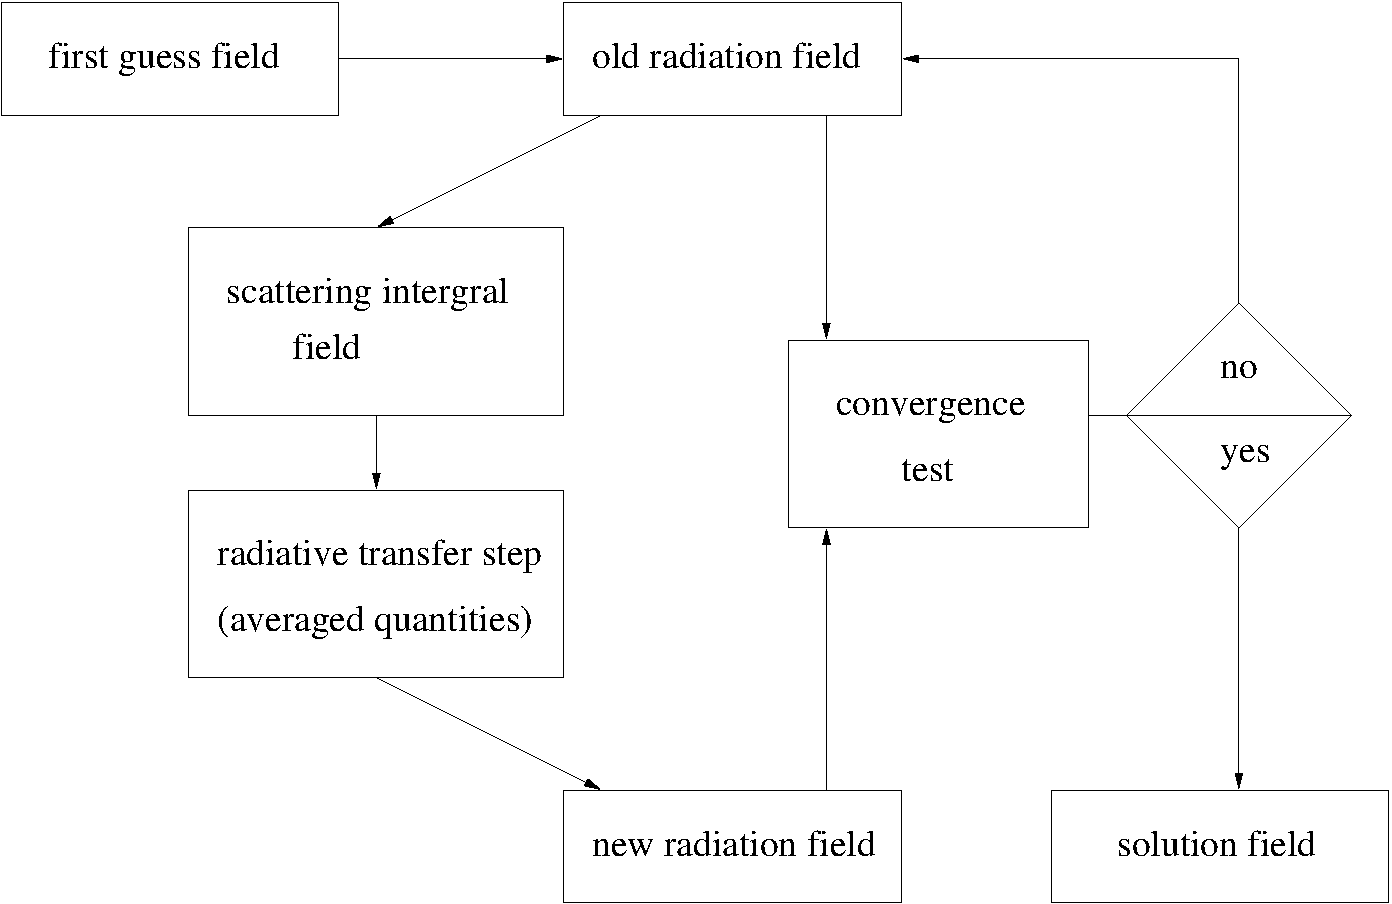
\includegraphics[width=.95\hsize]{iteration_scheme}}
  \caption{Schematic of the iterative method to solve the VRTE in the cloud box.}
  \label{fig:scattering:iteration_scheme}
\end{figure}

The \emph{first guess field}
\begin{equation}
  \IFld^{(0)} = \left\{\StoVec^{(0)}_{ijklm}\right\},
\end{equation}
is partly determined by the boundary condition given by the radiation
coming from the clear sky part of the atmosphere traveling into the
cloud box.  Inside the cloud box an arbitrary field can be chosen as a
first guess. In order to minimize the number of iterations it should
be as close as possible to the solution field.

The next step is to solve the scattering integrals
\begin{equation}
  \EnsAvr{\AmpMat^{(0)}_{ijklm}} = \int_{4\pi} \DiffD \PDir'
  \EnsAvr{\PhaMat_{ijklm}} \StoVec_{ijklm}^{(0)},
  \label{eq:scattering:scat-int}
\end{equation}
using the first guess field, which is now stored in a variable
reserved for the \emph{old radiation field}. For the integration we
use equidistant angular grids in order to save computation time (cf.
Section \ref{sec:doit:grid_opt_interp}).  The radiation field, which is
generally defined on finer angular grids ($\vec{\AzmAng},
\vec{\ZntAng}$), is interpolated on the equidistant angular grids.
The integration is performed over all incident directions $\PDir'$ for
each propagation direction $\PDir$.  The evaluation of the scattering
integral is done for all grid points inside the cloud box. The
obtained integrals are interpolated on $\vec{\AzmAng}$ and
$\vec{\ZntAng}$.  The result is the first guess \emph{scattering
  integral field} ${\mathcal S}^{0}$:
\begin{equation}
  \SFld^{(0)} = \left\{\EnsAvr{\SVec^{(0)}_{ijklm} }\right\}.  
\end{equation}

Figure \ref{fig:scattering:average} shows a propagation path step from a grid
point $\VctStl{P} = (\Prs_i, \Lat_j, \Lon_k)$ into direction $\PDir =
(\ZntAng_l, \AzmAng_m)$. The radiation arriving at $\VctStl{P}$ from the
direction $\PDir'$ is obtained by solving the linear
differential equation:
\begin{equation}
  \frac{\DiffD \StoVec^{(1)}}{\DiffD s} =
  -\overline{\EnsAvr\ExtMat}  \StoVec^{(1)} + \overline{\EnsAvr\AbsVec}\,  \bar{B}
  +\overline{\EnsAvr{\SVec^{(0)}}},
  \label{eq:scattering:vrte-fs-av}
\end{equation}
where $\overline{\EnsAvr\ExtMat}$, $\overline{\EnsAvr\AbsVec}$, $\bar{B}$ and $\overline{\EnsAvr{\SVec^{(0)}}} $ are \emph{averaged quantities}.  This equation
can be solved analytically for constant coefficients. Multi-linear
interpolation gives the quantities $\ExtMat', \AbsVec',
\SVec'$ and $T'$ at the intersection point $\VctStl{P}'$.  To calculate the radiative transfer from $\VctStl{P}'$ towards $\VctStl{P}$ all quantities are approximated by
taking the averages between the values at $\VctStl{P}'$ and $\VctStl{P}$. The average value of the temperature is used to get the
averaged Planck function $\bar{B}$.

\begin{figure}[t!]
  \centering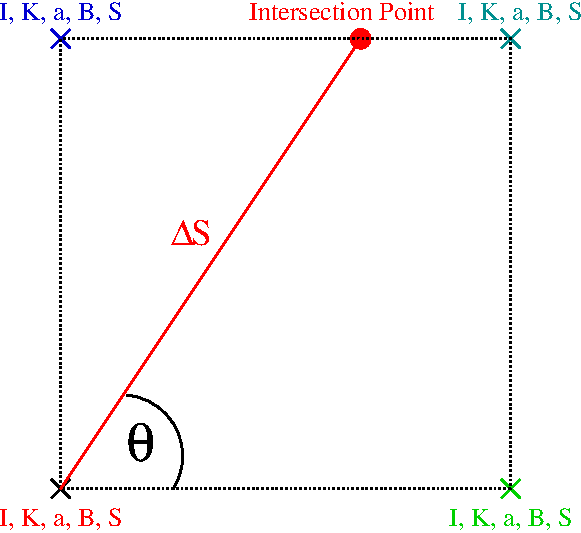
\includegraphics[width=.8\hsize]{average}
  \caption{Path from a grid point ($(\Prs_i, \Lat_j, \Lon_k)$~-~($\times$)) to the intersection point ($(\Prs_i', \Lat_j', \Lon_k')$~-~($\circ$)) with the next grid cell boundary. Viewing direction is specified by $(\ZntAng_l, \AzmAng_m)$ at ($\times$) or $(\ZntAng_l', \AzmAng_m')$ at ($\circ$).}
  \label{fig:scattering:average}
\end{figure}

The solution of Equation \ref{eq:scattering:vrte-fs-av} is found analytically using
a matrix exponential approach: % \FIXME  (see \appref{app:A}):
\begin{equation}
  \StoVec^{(1)} =
  e^{-\overline{\EnsAvr\ExtMat}  s} \StoVec^{(0)} + 
  \left( \IdnMtr -  e^{-\overline{\EnsAvr\ExtMat} s} \right)
  \overline{\EnsAvr\ExtMat}^{\,-1} \left(\overline{\EnsAvr\AbsVec}\,
    \bar{B} + \overline{\EnsAvr{\SVec^{(0)}}} \right),
  \label{eq:scattering:VRTE_sol}
\end{equation}
where \IdnMtr\ denotes the identity matrix and $\StoVec^{(0)}$ the
initial Stokes vector.  The \emph{radiative transfer step} from $\VctStl{P}'$ to $\VctStl{P}$ is calculated, therefore $\StoVec^{(0)}$ is
the incoming radiation at $\VctStl{P}'$ into direction
$(\ZntAng_l', \AzmAng_m')$, which is the first guess field
interpolated on $\VctStl{P}'$.  This radiative transfer step
calculation is done for all points inside the cloud box in all
directions. The resulting set of Stokes vectors ($\StoVec^{(1)}$ for
all points in all directions) is the first order iteration field
$\IFld^{(1)}$:
\begin{equation}
  \IFld^{(1)} = \left\{ \StoVec^{(1)}_{ijklm}\right\}.  
\end{equation}
The first order iteration field is stored in a variable reserved for the 
\emph{new radiation field}. 

In the \emph{convergence test} the \emph{new radiation field} is
compared to the \emph{old radiation field}. For the difference field,
the absolute values of all Stokes vector elements for all cloud box
positions are calculated. If one of the differences is larger than a
requested accuracy limit, the convergence test is not fulfilled. The
user can define different convergence limits for the different Stokes
components.

If the convergence test is not fulfilled, the first order iteration
field is copied to the variable holding the \emph{old radiation field}, 
and is then used to evaluate again the scattering integral at all
cloud box points:
\begin{equation}
  \EnsAvr{\SVec^{(1)}_{ijklm}} = \int_{4\pi} \DiffD \PDir'
  \EnsAvr\PhaMat \StoVec^{(1)}_{ijklm}.
\end{equation}
The second order iteration field
\begin{equation}
  \IFld^{(2)} = \left\{\StoVec^{(2)}_{ijklm}\right\},  
\end{equation}
is obtained by solving
\begin{equation}
  \frac{\DiffD \StoVec^{(2)}}{\DiffD s} =
  -\overline{\EnsAvr\ExtMat}  \StoVec^{(2)} + \overline{\EnsAvr\AbsVec}\,  \bar{B}
  +\overline{\EnsAvr{\SVec^{(1)}}},
\end{equation}
for all cloud box points in all directions.  This equation contains
already the averaged values and is valid for specified positions and
directions.

As long as the convergence test is not fulfilled the scattering integral fields and higher order iteration
fields are calculated alternately. 

We can formulate a differential equation for the $n$-th order
iteration field. The scattering integrals are given by
\begin{equation}
 \EnsAvr{\SVec^{(n-1)}_{ijklm}} = \int_{4\pi} \DiffD \PDir'
  \EnsAvr\PhaMat \StoVec^{(n-1)}_{ijklm},
\end{equation}
and the differential equation for a specified grid point into a
specified direction is
\begin{equation}
  \frac{\DiffD \StoVec^{(n)}}{\DiffD s} =
  -\overline{\EnsAvr\ExtMat}  \StoVec^{(n)} + \overline{\EnsAvr\AbsVec} \,\bar{B}
  +\overline{\EnsAvr{\SVec^{(n-1)}}}.
\end{equation}
Thus the \emph{$n$-th order iteration field }
\begin{equation}
  \IFld^{(n)} = \left\{ \StoVec^{(n)}_{ijklm} \right\},  
\end{equation}
is given by
\begin{equation}
  \StoVec^{(n)} =  e^{-\overline{\EnsAvr\ExtMat}
    s} + \cdot\StoVec^{(n-1)}  (\IdnMtr - e^{-\overline {\EnsAvr\ExtMat
    s}} ) \overline{\EnsAvr\ExtMat} ^{\,-1} ( \overline{\EnsAvr\AbsVec}\,\bar{B} + \overline{\EnsAvr{\SVec^{(n-1)}}} ),
\end{equation}
for all cloud box points and all directions defined in the numerical
grids.

If the convergence test
\begin{equation}
  \Abs{\StoVec^{(N)}_{ijklm} \left( \Prs_i, \Lat_j, \Lon_k, \ZntAng_l, \AzmAng_m\right)  -  \StoVec^{(N-1)}_{ijklm} \left( \Prs_i, \Lat_j, \Lon_k, \ZntAng_l, \AzmAng_m\right)} < \VctStl{\epsilon},
  \label{eq:scattering:conv_test}
\end{equation}
is fulfilled,
 a solution to the vector radiative transfer equation 
has been found:
\begin{equation}
  \IFld^{(N)} = \left\{ \StoVec^{(N)}_{ijklm} \right\}. 
\end{equation}



\section{Scalar radiative transfer equation solution}
\label{sec:doit:scattering:solution_rte_scalar}

In analogy to the \emph{scattering integral} vector field the scalar
scattering integral field is obtained:
\begin{equation}
  \EnsAvr{S^{(0)}_{ijklm}}  = \int_{4\pi} \DiffD \PDir' \EnsAvr{ Z_{11}} I^{(0)}_{ijklm}.
\end{equation}
The \emph{\textindex{scalar radiative transfer}} equation (compare
Equation~\ref{eq:rtetheory:SRTE}) with a
fixed scattering integral is
\begin{equation}
  \label{eq:scattering:SRTE-Int}
  \frac{\DiffD I^{(1)}}{\DiffD s} = -\EnsAvr{ K_{11}} I^{(1)}
  + \EnsAvr{a_1} B +\EnsAvr{S^{(0)}}.
\end{equation}
Assuming constant coefficients this equation is solved analytically
after averaging extinction coefficients, absorption coefficients,
scattering vectors and the temperature. The averaging procedure is done
analogously to the procedure described for solving the VRTE.  The
solution of the averaged differential equation is
\begin{equation}
\label{eq:scattering:SRTE_sol}
  I^{(1)} = I^{(0)} e^{-\overline{\EnsAvr{K_{11}}} s} +
  \frac{\overline{\EnsAvr{a_1}}\, 
    \bar{B} + \overline{\EnsAvr{ S^{(0)}}} }
  {\overline{\EnsAvr{ K_{11}}} }
  \left(1-e^{-\overline{\EnsAvr{K_{11}}} s}\right),
\end{equation}
where $I^{(0)}$ is obtained by interpolating the initial field, and
$\overline{\EnsAvr{K_{11}}}$, $\overline{\EnsAvr{a_1}}$,
$\bar{B}$ and $\overline{\EnsAvr{S^{(0)}}}$ are the
averaged values for the extinction coefficient, the absorption
coefficient, the 
Planck function and the scattering integral respectively.  Applying
this equation leads to the first iteration scalar intensity field,
consisting of the intensities $I^{(1)}$ at all points in the cloud box
for all directions.
  
As the solution to the vector radiative transfer equation, the solution
to the scalar radiative transfer equation is found numerically by the
same iterative method.  The convergence test for the scalar equation
compares the values of the calculated intensities of two successive
iteration fields.

\section{Single scattering approximation}
\label{sec:doit:ss_approx}

The DOIT method uses the \textindex{single scattering approximation},
which means 
that for one propagation path step the optical depth is assumed to be
much less than one so that multiple-scattering can be neglected along
this propagation path step. It is possible to choose a rather
coarse grid inside the cloud box. The user can define a limit
for the maximum propagation path step length. If a propagation path step from one
grid cell to the intersection point with the next grid cell boundary
is greater than this value, the path step is divided in several steps such
that all steps are less than the maximum value. The user has to make
sure that the optical depth due to particles for one propagation
path sub-step is is sufficiently small to assume
single scattering. The maximum optical depth due to particles along such a
propagation path sub-step is 
\begin{equation}
  \tau_{max} = \EnsAvr{\ExtMat^p} \cdot \Delta s_{max},
\end{equation}
where $\Delta s_{max}$ is the maximum length of a propagation path sub-step. In all
simulations presented in \citet{emde05:_phdthesis}, $\tau_{max} \ll$ 0.01 is
assumed. This threshold value is also used in \citet{czekala99:_microw}.
The radiative transfer calculation
is done along the propagation path through one grid cell.  All
coefficients of the VRTE are interpolated linearly on the propagation
path points.

\section{\textindex{Sequential update}}\label{chap:numerical_methods}
\label{sec:doit:sequential_update}

In the previous Sections, the iterative solution method
for the VRTE  
has been described. For each grid point inside the cloud box the
intersection point with the next grid cell boundary is determined in
each viewing direction.  After that, all the quantities involved in the
VRTE are interpolated onto this intersection point. As described in
the sections above, the intensity field of the previous iteration is
taken to obtain the Stokes vector at the intersection point.  Suppose
that there are $N$ pressure levels inside the cloud box.  If the
radiation field is updated taking into account for each grid point
only the adjacent grid cells, at least $N$-1 iterations are required
until the scattering effect from the lower-most pressure level has
propagated throughout the cloud box up to the uppermost pressure level.
From these considerations, it follows, that the number of iterations
depends on the number of grid points inside the cloud box.  This means
that the original method is very ineffective where a fine resolution
inside the cloud box is required to resolve the cloud inhomogeneities.

A solution to this problem is the ``sequential update of the radiation
field'', which is shown schematically in Figure \ref{fig:scattering:seq_update}.
For simplicity it will be explained in detail for a 1D cloud box. We
divide the update of the radiation field, i.e., the radiative transfer
step calculations for all positions and directions inside the
cloud box, into three parts: Update for ``up-looking'' zenith angles
(0$^\circ$ $\le$ $\ZntAng_\mathrm{up}$ $\le$ 90$^\circ$), for ``down-looking''
angles ($\ZntAng_\mathrm{limit}$ $\le$ $\ZntAng_\mathrm{down}$ $\le$ 180$^\circ$) and
for ``limb-looking'' angles (90$^\circ$ $<$ $\ZntAng_\mathrm{limb}$ $<$
$\ZntAng_\mathrm{limit}$). The ``limb-looking'' case is needed, because for
angles between 90$^\circ$\ and $\ZntAng_\mathrm{limit}$ the intersection point
is at the same pressure level as the observation point. The limiting
angle $\ZntAng_\mathrm{limit}$ is calculated geometrically.  Note that the
propagation direction of the radiation is opposite to the viewing
direction or the direction of the line of sight, which is indicated by the arrows.  In the
1D case the radiation field is a set of Stokes vectors each of which
depend upon the position and direction:
\begin{equation}
  \IFld = \left\{\StoVec \left( \Prs_i,\ZntAng_l \right) \right\}. 
\end{equation}

\begin{figure}[htbp]
\centering
  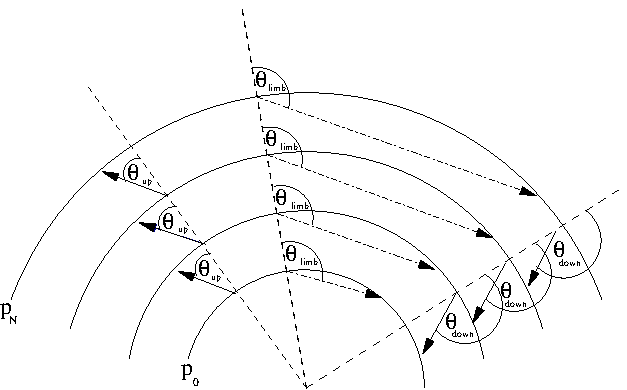
\includegraphics[width=.8\hsize]{seq_update_bw}
 \caption{Schematic of the sequential update (1D) showing the three different parts:  ``up-looking'' corresponds to zenith angles $\ZntAng_\mathrm{up}$, ``limb-looking'' corresponds to $\ZntAng_\mathrm{limb}$ ``down-looking'' corresponds to $\ZntAng_\mathrm{down}$.}
  \label{fig:scattering:seq_update}  
\end{figure}

The \emph{boundary condition} for the calculation is the incoming
radiation field on the cloud box boundary $\IFld^{bd}$:
\begin{eqnarray}
  \IFld^{bd} = \left\{\StoVec \left( \Prs_i,\ZntAng_l \right) \right\}
  \: \mathrm{where}  \: & \Prs_i = \Prs_N \, \forall \,  \ZntAng_l \in [0,\ZntAng_\mathrm{limit}]  \nonumber\\
   & \Prs_i = \Prs_0  \, \forall \, \ZntAng_l \in (\ZntAng_\mathrm{limit},180^\circ],
\end{eqnarray}
where $\Prs_0$ and $\Prs_N$ are the pressure coordinates of the lower and
upper cloud box boundaries respectively. For down-looking directions,
the intensity field at the lower-most cloud box boundary and for up-
and limb-looking directions the intensity field at the uppermost
cloud box boundary are the required boundary conditions respectively.

\subsection{Up-looking directions}

The first step of the sequential update is to calculate the intensity
field for the pressure coordinate $\Prs_{N-1}$, the pressure level below
the uppermost boundary, for all up-looking directions.  Radiative
transfer steps are calculated for paths starting at the uppermost
boundary and propagating to the ($N-1$) pressure level. The required
input for this radiative transfer step are the averaged coefficients
of the uppermost cloud box layer and the Stokes vectors at
the uppermost boundary for all up-looking directions. These are obtained
by interpolating the boundary condition $\IFld^{bd}$ on the
appropriate zenith angles. Note that the zenith angle of the
propagation path for the observing direction $\ZntAng_l$ does not equal
$\ZntAng_l'$ at the intersection point due to the spherical
geometry. If $\ZntAng_l$ is close to $90^\circ$\ this difference is
most significant.
  
To calculate the intensity field for the pressure coordinate
$\Prs_{N-2}$, we repeat the calculation above. We have to calculate a
radiative transfer step from the ($N-1$) to the ($N-2$) pressure level.
As input we need the interpolated intensity field at the ($N-1$)
pressure level, which has been calculated in the last step.
  
For each pressure level ($m-1$) we take the interpolated field of the
layer above ($\IFld(\Prs_{m})^{(1)}$).  Using this method, the
scattering influence from particles in the upper-most cloud box
layer can propagate during one iteration down to the lower-most layer.
This means that the number of iterations does not scale with the
number of pressure levels, which would be the case without sequential
update.
  
The radiation field at a specific point in the cloud box is obtained by
solving Equation \ref{eq:scattering:VRTE_sol}. For up-looking directions at position
$\Prs_{m-1}$ we may write:
\begin{eqnarray}
 & \StoVec\left( \Prs_{m-1},\ZntAng_\mathrm{up} \right) ^{(1)}  =  
  e^{-\overline{\EnsAvr{\ExtMat (\ZntAng_\mathrm{up})}} s} 
  \StoVec\left( \Prs_m,\ZntAng_\mathrm{up} \right)^{(1)}  \nonumber \\ &+
  \left( \IdnMtr -  e^{-\overline{\EnsAvr{\ExtMat (\ZntAng_\mathrm{up})}} s}\right) 
  \overline{\EnsAvr{\ExtMat(\ZntAng_\mathrm{up})}}^{\,-1} 
  \left( \overline{\EnsAvr{\AbsVec (\ZntAng_\mathrm{up})}}\,  
    \bar{B} +
    \overline{\EnsAvr{\SVec\left(\ZntAng_\mathrm{up} \right)^{(0)}} }
  \right).
\end{eqnarray}
For simplification we write
\begin{equation}
  \StoVec ( \Prs_{m-1},\ZntAng_\mathrm{up})^{(1)} = 
  \MtrStl{A}(\ZntAng_\mathrm{up})  \StoVec\left( \Prs_m,\ZntAng_\mathrm{up} \right)^{(1)} 
  + \MtrStl{B} ( \ZntAng_\mathrm{up}).
\end{equation}
Solving this equation sequentially, starting at the top of the cloud
and finishing at the bottom, we get the updated radiation field for
all up-looking angles.
\begin{equation} \IFld(\Prs_i, \ZntAng_\mathrm{up})^{(1)} =
  \left\{ \StoVec^{(1)} \left( \Prs_i,\ZntAng_l \right) \right\} \qquad
  \forall \; \ZntAng_{l} \in [0, 90^\circ].
\end{equation}

\subsection{Down-looking directions}
The same procedure is done for down-looking directions.  The only
difference is that the starting point is the lower-most pressure level
$\Prs_1$ and the incoming clear sky field at the lower cloud box boundary,
which is interpolated on the required zenith angles, is taken as
boundary condition.  The following equation is solved sequentially,
starting at the bottom of the cloud box and finishing at the top:
\begin{equation}
  \StoVec ( \Prs_{m},\ZntAng_\mathrm{down} ) ^{(1)} = 
  \MtrStl{A}(\ZntAng_\mathrm{down}) \StoVec\left( \Prs_{m-1},\ZntAng_\mathrm{down} \right)^{(1)} 
  + \MtrStl{B}(\ZntAng_\mathrm{down}).
\end{equation}
This yields the updated radiation field for all down-looking angles.
\begin{equation}
  \IFld(\Prs_i, \ZntAng_\mathrm{down})^{(1)} = \left\{ \StoVec^{(1)} \left( \Prs_i,\ZntAng_l \right) \right\}  \qquad
  \forall \;  \ZntAng_l \in [\ZntAng_\mathrm{limit}, 180^\circ].
\end{equation}

\subsection{Limb directions}
A special case for limb directions, which correspond to angles
slightly above 90$^\circ$\, had to be implemented.  If the tangent
point is part of the propagation path step, the intersection point is
exactly at the same pressure level as the starting point.  In this
case the linearly interpolated clear sky field is taken as input for
the radiative transfer calculation, because we do not have an already
updated field for this pressure level:
\begin{equation}
  \StoVec ( \Prs_{m},\ZntAng_\mathrm{limb} ) ^{(1)} =   
  \MtrStl{A}(\ZntAng_\mathrm{limb}) \StoVec\left( \Prs_{m},\ZntAng_\mathrm{limb} \right)^{(0)} 
  + \MtrStl{B}(\ZntAng_\mathrm{limb})
\end{equation}
By solving this equation the missing part of the updated radiation
field is obtained
\begin{equation}
  \IFld(\Prs_i, \ZntAng_\mathrm{limb})^{(1)} = \left\{\StoVec \left( \Prs_i,\ZntAng_l \right) \right\}  \qquad
  \forall \;  \ZntAng_l \in  ]90^\circ, \ZntAng_\mathrm{limit}[
\end{equation}
For all iterations the sequential update is applied. Using this method
the number of iterations depends only on the optical thickness of the
cloud or on the number of multiple-scattering events, not on the
number of pressure levels.


\section{Numerical Issues}
\label{sec:doit:implementation_DOIT}


\subsection{Grid optimization and interpolation}
\label{sec:doit:grid_opt_interp}

The accuracy of the DOIT method depends very much on the
discretization of the zenith angle. The reason is that the intensity
field strongly increases at about $\ZntAng=90^\circ$. For angles
below 90$^\circ$ (``up-looking'' directions) the intensity is very
small compared to angles above 90$^\circ$ (``down-looking''
directions), because the thermal emission from the lower atmosphere
and from the ground is much larger than thermal emission from trace
gases in the upper atmosphere. Figure \ref{fig:scattering:i_field} shows an
example intensity field as a function of zenith angle for different
pressure levels inside a cloud box, which is placed from 7.3 to 12.7\,km
altitude, corresponding to pressure limits of 411\,hPa and 188\,hPa
respectively. The cloud box includes 27 pressure levels. The frequency
of the sample calculation was 318\,GHz. A midlatitude-summer scenario
including water vapor, ozone, nitrogen and oxygen was used.
The atmospheric data was taken from the FASCOD \citep{anderson:86}
and the spectroscopic data was obtained from the HITRAN database
\citep{rothman:98}. For simplicity 
this 1D set-up was chosen for all sample calculations in this section.  As the
intensity (or the Stokes vector) at the intersection point of a
propagation path is obtained by interpolation, large interpolation
errors can occur for zenith angles of about 90$^\circ$ if the zenith
angle grid discretization is too coarse.  Taking a very fine
equidistant zenith angle grid leads to very long computation times.
Therefore a zenith angle grid optimization method is required.

For the computation of the scattering integral it is possible to take
a much coarser zenith angle resolution without losing accuracy.  It
does not make sense to use the zenith angle grid, which is optimized
to represent the radiation field with a certain accuracy. The
integrand is the product of the phase matrix and the radiation field.
The peaks of the phase matrices can be at any zenith angle, depending
on the incoming and the scattered directions. The multiplication
smooths out both the radiation field increase at 90$^\circ$ and the
peaks of the phase matrices.  Test calculations have shown that an
increment of 10$^\circ$ is sufficient. Taking the equidistant grid
saves the computation time of the scattering integral to a very large
extent, because much less grid points are required.

\begin{figure}[htbp]
\centering
  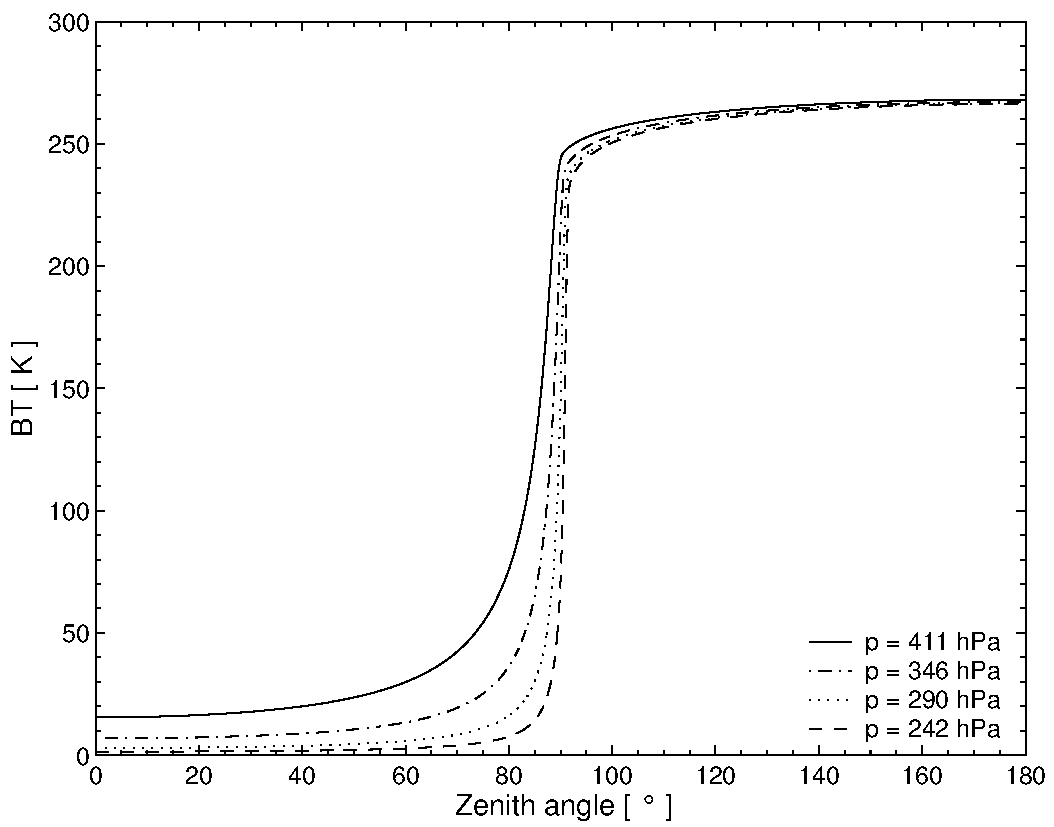
\includegraphics[width=0.8\hsize]{i_field}
  \caption{Intensity field for different pressure levels.}
  \label{fig:scattering:i_field}  
\end{figure}


\subsection{Zenith angle grid optimization}

As a reference field for the grid optimization the DOIT method is
applied for an empty cloud box using a very fine zenith angle grid. The
grid optimization routine finds a reduced zenith angle grid which can
represent the intensity field with the desired accuracy.  It first
takes the radiation at 0$^\circ$ and 180$^\circ$ and interpolates
between these two points on all grid points contained in the fine
zenith angle grid for all pressure levels. Then the differences
between the reference radiation field and the interpolated field are
calculated. The zenith angle grid point, where the difference is
maximal is added to 0$^\circ$ and 180$^\circ$. After that the
radiation field is interpolated between these three points forming 
part of the reduced grid and again the grid point with the maximum
difference is added. Using this method more and more grid points are
added to the reduced grid until the maximum difference is below a
requested accuracy limit.

The top panel of Figure \ref{fig:scattering:grid_acc} shows the clear sky
radiation in all viewing directions for a sensor located at 13\,km
altitude. This result was obtained with a switched-off cloud box.  The
difference between the clear sky part of the ARTS model and the
scattering part is that in the clear sky part the radiative transfer
calculations are done along the line of sight of the instrument
whereas inside the cloud box the RT calculations are done as described
in the previous section to obtain the full radiation field inside the
cloud box. In the clear sky part the radiation field is not
interpolated, therefore we can take the clear sky solution as the exact
solution.

\begin{figure}[t]
\centering
  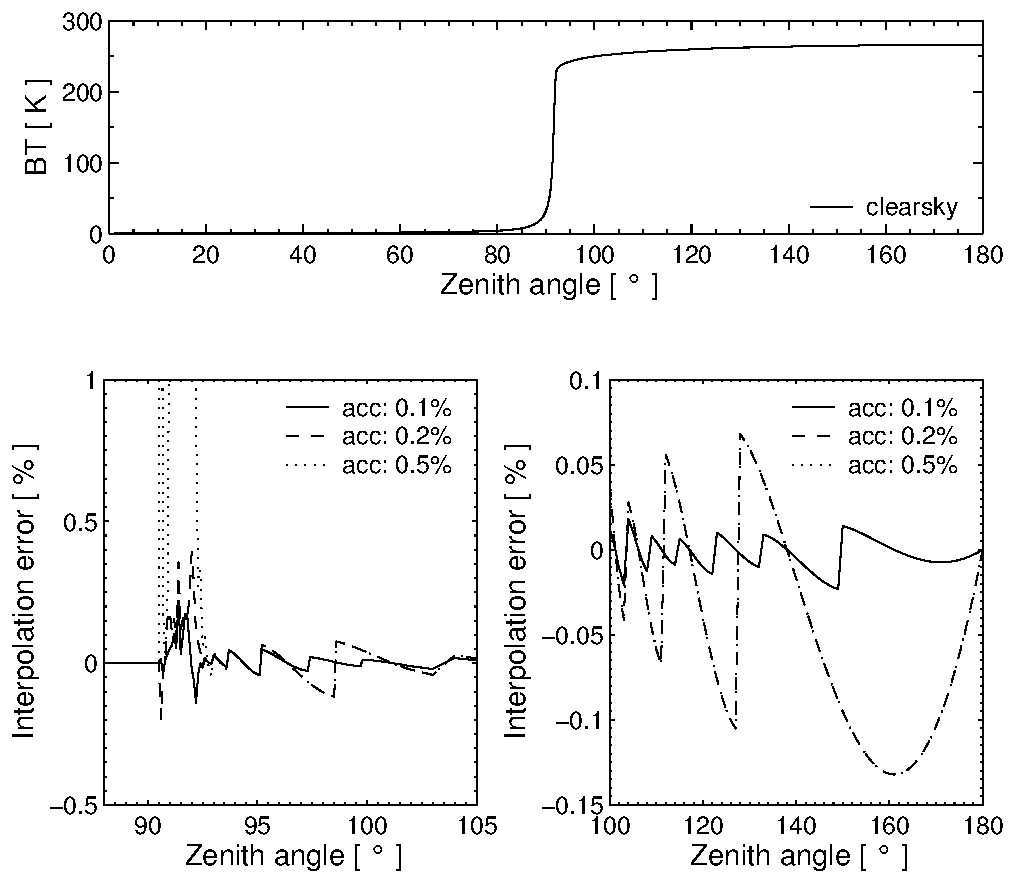
\includegraphics[width=.9\hsize]{grid_acc}
  \caption{Interpolation errors for different grid accuracies.
    Top panel: Clear sky radiation simulated for a sensor at an altitude of
    13\,km for all viewing directions.
    Bottom left: Grid optimization accuracy for limb directions.
    Bottom right: Grid optimization accuracy for down-looking
    directions.}
  \label{fig:scattering:grid_acc}  
\end{figure}

The interpolation error is the relative difference between the exact
clear sky calculation (cloud box switched off) and the clear sky
calculation with empty cloud box.  The bottom panels of
Figure \ref{fig:scattering:grid_acc} show the interpolation errors for zenith
angle grids optimized with three different accuracy limits (0.1\%,
0.2\% and 0.5\%.). The left plot shows the critical region close to
90$^\circ$.  For a grid optimization accuracy of 0.5\% the
interpolation error becomes very large, the maximum error is 
about 8\%. For grid accuracies of 0.2\% and 0.1\% the maximum
interpolation errors are about 0.4\% and 0.2\% respectively. However
for most angles it is below 0.2\%, for all three cases. For
down-looking directions from 100$^\circ$ to 180$^\circ$ the
interpolation error is at most 0.14\% for grid accuracies of 0.2\% and 0.5\%
and for a grid accuracy of 0.1\% it is below~0.02\%. 


\subsection{Interpolation methods}
Two different interpolation methods can be chosen in ARTS for the
interpolation of the radiation field in the zenith angle dimension:
linear interpolation or three-point polynomial interpolation. The polynomial interpolation
method produces more accurate results provided that the zenith angle
grid is optimized appropriately. The linear interpolation method on
the other hand is safer. If the zenith angle grid is not optimized for
polynomial interpolation one should use the simpler linear interpolation
method.  Apart from the interpolation of the radiation field in the
zenith angle dimension linear interpolation is used everywhere in the
model.  Figure \ref{fig:scattering:interp} shows the interpolation errors for the
different interpolation methods.  Both calculations are performed on
optimized zenith angle grids, for polynomial interpolation 65 grid points
were required to achieve an accuracy of 0.1\% and for linear
interpolation 101 points were necessary to achieve the same accuracy.
In the region of about 90$^\circ$ the interpolation errors are below
1.2\% for linear interpolation and below 0.2\% for polynomial
interpolation. For the other down-looking directions the differences
are below 0.08\% for linear and below 0.02\% for polynomial interpolation.
It is obvious that polynomial interpolation gives more accurate results.
Another advantage is that the calculation is faster because less grid
points are required, although the polynomial interpolation method itself is
slower than the linear interpolation method.  Nevertheless, we have
implemented the polynomial interpolation method so far only in the 1D
model. In the 3D model, the grid optimization needs to be done over
the whole cloud box, where it is not obvious that
one can save grid points. Applying the polynomial interpolation method
using non-optimized grids can yield much larger interpolation errors
than the linear interpolation method.

\begin{figure}[htbp]
\centering
  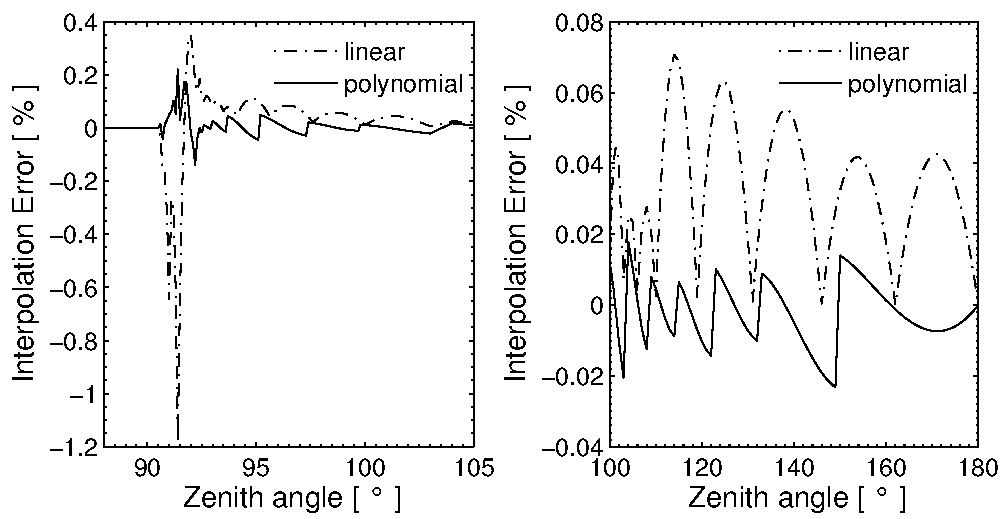
\includegraphics[width=.9\hsize]{interp}
  \caption{Interpolation errors for polynomial and linear interpolation.
  }
  \label{fig:scattering:interp}  
\end{figure}

\subsection{Error estimates}
The interpolation error for scattering calculations can be estimated
by comparison of a scattering calculation performed on a very fine
zenith angle grid (resolution 0.001$^\circ$ from 80$^\circ$ to
100$^\circ$) with a scattering calculation performed on an optimized
zenith angle grid with 0.1\% accuracy. The cloud box used in previous
test calculations is filled with spheroidal particles with an aspect
ratio of 0.5 from 10 to 12\,km altitude. The ice mass content is
assumed to be $4.3\cdot10^{-3}$\,g/m$^3$ at all pressure levels.  
An equal volume sphere radius of 75$\,\mum$ is assumed. The particles are
either completely randomly oriented ("totally\_random") or horizontally aligned
(a special case of "azimuthally\_random" oriented particles) (cf. \user, Section
\ref{U-sec:clouds:particle_types}). The top panels of
Figure \ref{fig:scattering:interp_err} show the interpolation errors of the
intensity.  For both particle orientations the interpolation error is
in the same range as the error for the clear sky calculation, below
0.2\,K. The bottom panels show the interpolation errors for~$Q$. For the
randomly oriented particles the error is below 0.5\%. For the
horizontally aligned particles with random azimuthal orientation it goes up to 2.5\% for a
zenith angle of about 91.5$^\circ$. It is obvious that the
interpolation error for~$Q$ must be larger than that for~$I$ because the
grid optimization is accomplished using only the clear-sky field,
where the polarization is zero. Only the limb directions about
90$^\circ$ are problematic, for other down-looking directions the
interpolation error is below~0.2\%.

\begin{figure}[htbp]
  \centering
  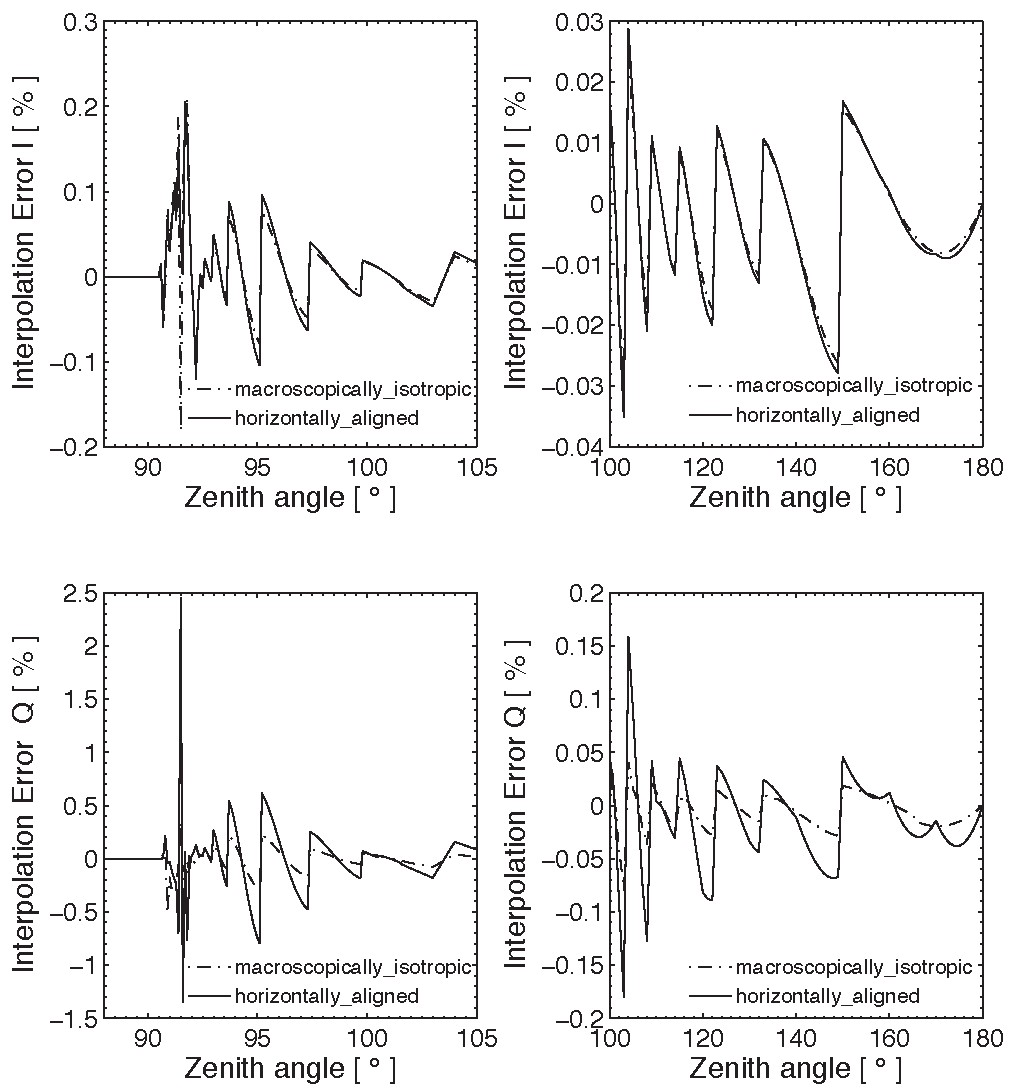
\includegraphics[width=.9\hsize]{interp_err}
  \caption{Interpolation errors for a scattering calculation.
    Left panels: Interpolation errors for limb directions.
    Right panels: Interpolation errors for down-looking directions.
    Top: Intensity~$I$, Bottom: Polarization difference~$Q$}
  \label{fig:scattering:interp_err}  
\end{figure}


\graphicspath{{Figs/montecarlo/}}

%
% To start the document, use
%  \chapter{...}
% For lover level, sections use
%  \section{...}
%  \subsection{...}
%
\chapter{Reversed Monte Carlo Scattering: ARTS-MC}
 \zlabel{sec:montecarlo}


%
% Document history, format:
%  \starthistory
 %    date1 & text .... \\
%    date2 & text .... \\
%    ....
%  \stophistory
%
\starthistory
  120410 & Moved from user guide to theory document.\\
  300504 & Created and written by Cory Davis.\\
\stophistory


%
% Symbol table, format:
%  \startsymbols
%    ... & \verb|...| & text ... \\
%    ... & \verb|...| & text ... \\
%    ....
%  \stopsymbols
%
%

%
% Introduction
%




\section{Introduction}
 \zlabel{sec:montecarlo:intro}

%%%%%%%%%%%%%%%%%%%%%%%%%%%%%%%%%%%%%%%%%%%%%%%%%%%%%%%%%% 
\section{Model[FIXME: needs updating to MCGeneral]}
 \zlabel{sec:montecarlo:model}
The radiative transfer model solves the vector
radiative transfer equation (VRTE):
\begin{eqnarray}
\frac{d\mathbf{I(n)}}{ds}=-\mathbf{K(n)I(n)} +
\mathbf{K_a(n)}I_b(T) +\nonumber\\
\int_{4\pi}\mathbf{Z(n,n')I(n')}d\mathbf{n'}
\zlabel{vrte}
\end{eqnarray}
where $\mathbf{I}$ is the 4 element column vector of radiances
$\mathbf{I}=\left[I,Q,U,V\right]^T$ with units
(Wm$^{-2}\mu$m$^{-1}$sr$^{-1}$). This will be referred to as the
Stokes vector, although normally the Stokes vector is expressed in
units of intensity.  $s$ is distance along direction $\mathbf{n}$ and
$I_b$ is the Planck radiance. $\mathbf{K(n)}$, $\mathbf{K_a(n)}$,
and $\mathbf{Z(n,n')}$ are the bulk extinction matrix, absorption
coefficient vector and phase matrix of the medium respectively.  For
 brevity these have been expressed as bulk optical
properties, where individual single scattering properties have been
multiplied by particle number density and averaged over all
orientations and particle types. The argument $\mathbf{n}$ has been
retained to signify that in general these properties depend on the
direction of propagation. 

To apply Monte Carlo integration to the problem, the VRTE needs to be expressed in integral form. (e.g. \cite{hochstadt:64})
\begin{eqnarray}
\lefteqn{\mathbf{I(n,s_0)}=\mathbf{O(u_0,s_0)I(n,u_0)}+}\nonumber\\
& \int_{u_0}^{s_0}\mathbf{O(s',s_0)}\left(\mathbf{K_a(n)}I_b(T) +\int_{4\pi}\mathbf{Z(n,n')}\mathbf{I(n')}d\mathbf{n'}\right)ds'\nonumber
\end{eqnarray}
\begin{equation}
\zlabel{intVRTE}
\end{equation}
, where $\mathbf{O(s',s)}$ is the evolution operator defined by
\cite{landi:85}. $\mathbf{u_0}$ is the point where the line of sight intersects
the far boundary of the scattering domain, and $\mathbf{s_0}$ is the
exit point where the outgoing Stokes vector is calculated.
In general there is no closed form expression for $\mathbf{O(s',s)}$.
However, in cases where the extinction matrix is constant along a
propagation path
\begin{equation}
\mathbf{O(s',s)}=\exp\left(-\mathbf{K}\Delta s\right)
\zlabel{OconstK}
\end{equation}
In ARTS a propagation path consists of a set of coordinates
indicating where the path intersects with grid surfaces.  If the
extinction matrix in the path segment between two such points is
considered constant, $\mathbf{K}=(\mathbf{K_j}+\mathbf{K_{j+1}})/2$,
the evolution operator between two arbitrary points $\mathbf{s_0}$ and
$\mathbf{s}_N$ is
\begin{eqnarray}
\mathbf{O}(\mathbf{s}_0,\mathbf{s}_N) =
\mathbf{O}(\mathbf{s}_{N-1},\mathbf{s}_N)
\mathbf{O}(\mathbf{s}_{N-2},\mathbf{s}_{N-1}) \dots \nonumber\\
\mathbf{O}(\mathbf{s}_1,\mathbf{s}_2)\mathbf{O}(\mathbf{s}_0,\mathbf{s}_1),
\end{eqnarray}
, where $\mathbf{O(s_i,s_{i+1})}$ is given by Eq. \zref{OconstK}.

The numerical task is then to perform Monte Carlo
integration on the integral on the right hand side of
Eq. \zref{intVRTE}.
The aim in importance sampling is to choose probability density functions
(PDFs) for the independent variables that are
as close as possible to being proportional to the integrand
\cite{liu:01}. This concentrates computational effort on regions where
the integrand is most significant and also reduces the variance in the contributions of each photon, thus reducing
the number of photons and hence CPU time required to give a
prescribed accuracy.  Eq. \zref{intVRTE} suggests that the PDF for
sampling path length, where path length is the distance traced backwards
from the sensor, $\Delta s=\left|\mathbf{s}-\mathbf{s'}\right|$, should be proportional in some way to the evolution
operator $\mathbf{O(s',s)}$. Likewise, new incident directions
($\theta_{inc},\phi_{inc}$) should be sampled from a PDF proportional
to
$\mathbf{Z}(\theta_{scat},\phi_{scat},\theta_{inc},\phi_{inc})$.
Since PDFs are scalar functions, and that we consider the first element of the
Stokes vector most important, we choose PDFs that are proportional to the
(1,1) element of $\mathbf{O(s',s)}$ and $\mathbf{Z}(\theta_{scat},\phi_{scat},\theta_{inc},\phi_{inc})$. 
%%%%%%%%%%%%%%%%%%%%%%%%%%%%%%%%%%%%%%%%%%%%%%%%%%%%%%%%%%%%%
\subsection{Algorithm [FIXME:Needs updating to MCGeneral]}
 \zlabel{sec:montecarlo:alg}
The model algorithm proceeds as follows:

\begin{enumerate}
\item
Begin at the cloud box exit point with a new photon. Sample a
  path length, $\Delta s$ along the first line of sight using the PDF
\begin{equation}
g_0(\Delta s)=\frac{\tilde{k}\tilde{O_{11}}(\Delta s)}
{1-O_{11}(\mathbf{u_0,s_0})}.
\zlabel{g0Deltas}
\end{equation}
, where $\tilde{O_{11}}(\Delta s)$, is the piecewise exponential
function that includes $O_{11}(\mathbf{s',s})$ values at points
where the line of sight intersects with grid surfaces.
Between two such adjacent intersections, $A$ and $B$, the function
$\tilde{O_{11}}(\Delta s)$ is given by
\begin{equation}
\tilde{O_{11}}(\Delta s)=O_{11}(\Delta s_A)\exp\left(-\tilde{k}\left(\Delta s-\Delta
s_A\right)\right)
\zlabel{O11}
\end{equation}
, and
\begin{equation}
\tilde{k}=\frac{1}{\left(\Delta s_B-\Delta s_A\right)}
\ln\left(\frac{O_{11}^A}{O_{11}^B}\right)
\end{equation}
, which, for cases where the extinction matrix is diagonal, is equal to $K_{11}=(K_{11}^A+K_{11}^B)/2$.
The denominator in Eq. \zref{g0Deltas} ensures an emission or scattering
event for each photon in the initial line of sight.
Eq. \zref{g0Deltas} is sampled by taking a random number (from the
uniform distribution [0,1]), $r$, and solving 
\begin{equation}
\frac{1-\tilde{O_{11}}(\Delta s)}{1-O_{11}(\mathbf{u_0,s_0})}=r.
%\zlabel{solvefor0}
\end{equation}
for $\Delta s$.
%%%%%%%%%%%%%%%%%%%%%%%%%%%%%%%%%%%%%%%%%%%%%%%%%%%%%%%%%%%%%%%%
\item
Another random number, $r$, is drawn to choose between emission and scattering.  We first define an albedo-like quantity
\begin{equation}
\tilde{\omega}=1-\frac{K_{a1}(\mathbf{n_{0},s_{1}})}{K_{11}(\mathbf{n_{0},s_{1}})}
\end{equation}
Note: we can't use the actual single-scattering albedo as this depends
on the polarization state of the incident radiation.  If $r>\tilde{\omega}$, then the event is considered to be emission,
the reversed ray tracing is terminated, and the Stokes vector
contribution of the $i$th photon is
\begin{equation}
\mathbf{I^i(n,s_0)}=\frac{\mathbf{O(s_1,s_0)}\mathbf{K_a(n_0,s_1)}
  I_b(T,\mathbf{s_i})}{g_0(\Delta s) \left(1-\tilde{\omega}\right)}
\zlabel{Iemission2}
\end{equation}
, where the index $i$ signifies photon number. Return to step 1.

Otherwise, if $r\le\tilde{\omega}$
we have a scattering event.
%3%%%%%%%%%%%%%%%%%%%%%%%%%%%%%%%%%%%%%%%%%%%%%%%
\item
At the scattering point sample a new incident direction
  $(\theta_{inc},\phi_{inc})$ according to 
\begin{equation}
g(\theta_{inc},\phi_{inc})=\frac{Z_{11}(\theta_{scat},\phi_{scat},
\theta_{inc},\phi_{inc})\sin(\theta_{inc})}{K_{11}(\theta_{scat},\phi_{scat})
  - K_{a1}(\theta_{scat},\phi_{scat})}
\zlabel{gdir}
\end{equation}
, which is
sampled by the rejection method as described in \cite{liu:01}.

Calculate the matrix
\begin{equation}
\mathbf{Q_k}=\mathbf{Q_{k-1}q_k}
\zlabel{Q}
\end{equation}
, where
\begin{equation}
\mathbf{q_k}=\frac{\sin(\theta_{inc})_k
  \mathbf{O(s_k,s_{k-1})}\mathbf{Z(n_{k-1},n_k)}}
  {g\left(\Delta s\right)g(\theta_{inc},\phi_{inc}) \tilde{\omega}} ,
\zlabel{q}
\end{equation}
and $\mathbf{Q_0}={1}$. The index $k$ represents the
scattering order.
%4%%%%%%%%%%%%%%%%%%%%%%%%%%%%%%%%%%%%%%%%%%%%%%%%%%
\item
Choose a path length along the new direction according to
\begin{equation}
g(\Delta s)=\tilde{k}\tilde{O_{11}}(\Delta s)
\zlabel{gDeltas}
\end{equation}
This is sampled by taking a random number and solving 
\begin{equation}
\tilde{O_{11}}(\Delta s)=r.
%\zlabel{solvefor0}
\end{equation}
for $\Delta s$.
If $r<O_{11}(\mathbf{u_{k},s_k})$, where $\mathbf{u}_{k}$ is the
  boundary of the scattering domain in the current line of sight, the
  photon leaves the scattering domain, and the contribution for photon $i$ is
\begin{equation}
\mathbf{I^i(n,s_0)}=\frac{\mathbf{Q_k}\mathbf{O(u_k,s_k)I(n_k,u_k)}}{O_{11}(\mathbf{u_{k},s_k})}
\zlabel{Ikmax2_1}
\end{equation}
, where 
$\mathbf{I(n_k,u_k)}$ is the incoming radiance at $\mathbf{u}_{k}$.  This is calculated with the standard ARTS clear-sky
routine. Return to step 1.

Otherwise, if the sampled path length keeps the path within the
scattering domain...
%%%%%%%%%%%%%%%%%%%%%%%%%%%%%%%%%%%%%%%%%%%%%%%%%%%%%
\item
As in step 2, calculate 
$\tilde{\omega}$ at the new point, $\mathbf{s_{k+1}}$, and draw a uniform
  random deviate, $r$.

If $r>\tilde{\omega}$, then the event is considered to be emission,
the reversed ray tracing is terminated, the Stokes vector contribution is
\begin{equation}
\mathbf{I^i(n,s_0)}=\frac{\mathbf{Q_k O(s_{k+1},s_k)}
  \mathbf{K_a(n_k,s_{k+1})} I_b(T,\mathbf{s_{k+1}})}
  {g\left(\Delta s\right)\left(1-\tilde{\omega}\right)}
\zlabel{Iemission3}
\end{equation}
, and we return to step 1.

Otherwise, if $r\le\tilde{\omega}$
we have a scattering event and we return to step 3.
\item
Once the prescribed number, $N$,  of photon contributions,
$\mathbf{I^i(n,s_0)}$, have been calculated, the cloud box exit Stokes
vector is given by
\begin{equation}
\mathbf{I(n,s_0)}=\mathbf{O(u_0,s_0)I(n,u_0)}+\langle\mathbf{I^i(n,s_0)}\rangle.
\zlabel{cbexit}
\end{equation}
, with an estimated error for each Stokes index, $j$,  of
\begin{equation}
\delta I_j=\sqrt{\frac{\langle I_j^2\rangle-\langle I_j\rangle^2}{N}}.
\zlabel{error}
\end{equation}
\end{enumerate}
When simulating an MLS measurement, an extra clear sky RT calculation
is performed from the cloud box exit to the sensor, with the Monte
Carlo result from Eq. \zref{cbexit} taken as the radiative background.

\begin{figure}[!ht]
\begin{center}
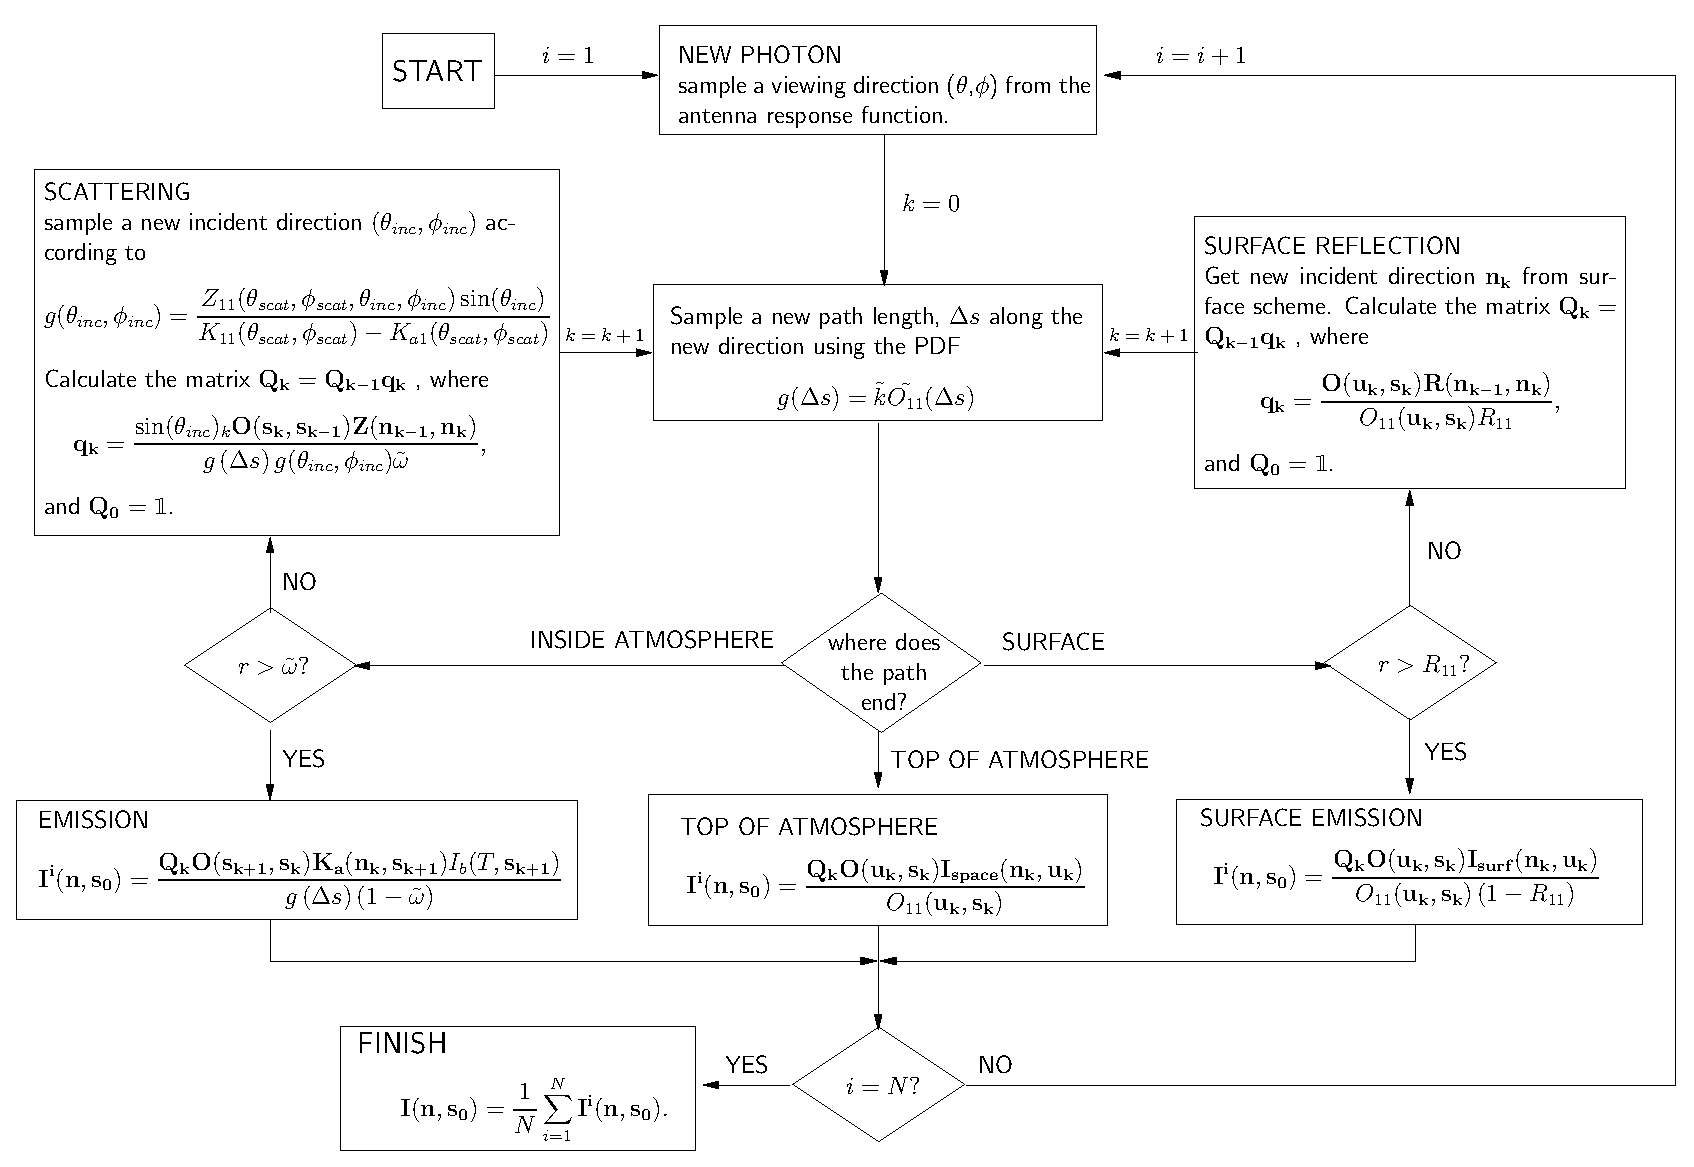
\includegraphics[width=\vsize,angle=90]{flowchart2}
\caption{Flowchart illustrating MCGeneral algorithm}
\end{center}
\zlabel{fig:montecarlo:flowchart}
\end{figure}

 
%%% Local Variables: 
%%% mode: latex 
%%% TeX-master: "uguide" 
%%% End:




\part{Bibliography and Appendices}
%
\bibliography{references}


\part{Index}
%
\printindex


%===   End of report   =====================================================
\end{document}


%%% Local Variables: 
%%% mode: latex
%%% TeX-master: t
%%% End: 
